\documentclass{book}
\usepackage{graphicx} % Required for inserting images
\usepackage{hyperref}
\usepackage{amsmath}
\usepackage{capt-of}
\usepackage{enumitem}

\usepackage{xcolor}
\definecolor{ipython_cyan}{RGB}{64, 128, 128}
\definecolor{maroon}{cmyk}{0, 0.87, 0.68, 0.32}
\definecolor{halfgray}{gray}{0.55}
\definecolor{ipython_frame}{RGB}{207, 207, 207}
\definecolor{ipython_bg}{RGB}{247, 247, 247}
\definecolor{ipython_red}{RGB}{186, 33, 33}
\definecolor{ipython_green}{RGB}{0, 128, 0}
\definecolor{ipython_purple}{RGB}{170, 34, 255}

\usepackage{listings} % package for code blocks
\lstset{language=Python,
frame=single,
basicstyle=\scriptsize\ttfamily,
breaklines=true,
keepspaces=true,
commentstyle=\color{halfgray}\itshape\ttfamily,
keywordstyle=\color{ipython_green}\bfseries\ttfamily,
identifierstyle=\color{black}\ttfamily,
stringstyle=\color{ipython_red}\ttfamily
%numbers=left,
%stepnumber=2,
%numberstyle=\tiny\color{halfgray},s
%framexleftmargin=6mm
}
\title{Nanodegree Introduction to Deep Learning}
\author{Susanna Olinda Kusrini}
\date{January 2023}

\begin{document}

\maketitle
\tableofcontents

\part{Convolutional Neural Networks}
\chapter{Introduction to CNNs}
\href{https://www.youtube.com/watch?v=-dLdeL6BAZs&t=1s&ab_channel=Udacity}{Youtube} \newline

A CNN is a neural network developed specifically for image and video processing. CNNs are used to automate many tasks, for example:

\begin{itemize}
    \item Image classification
    \item Object recognition
    \item Anomaly detection
    \item Image captioning
\end{itemize}
... and many others. They are widely used across many industries, including medicine, banking, manufacturing, insurance, real-estate, transportation (self-driving cars), and social networks.\newline

CNNs are arguably the main technology responsible for the Artificial Intelligence renaissance we are witnessing today, with billion of dollars in revenue generated by their application.\newline

We are very excited for you to be here with us and to learn about this invaluable technology!


\section{Course Overview}

\begin{itemize}
    \item Introduction to CNNs and basic concepts

\begin{itemize}
        \item Use Multi-Layer Perceptrons (MLPs) for image classification
        \item Understand the limitations of MLPs for images and how CNNs overcome them
        \item Learn basic concepts of CNNs and what makes them so powerful for image tasks
\end{itemize}

    \item CNNs in more depth

\begin{itemize}
        \item Learn all the basic layers that make up a CNN
        \item Put all the basic layers together to build a CNN from scratch
        \item Classify images using CNNs
        \item Use various methods to improve CNN performance
        \item Export models for production
\end{itemize}

    \item Transfer learning

\begin{itemize}
        \item Understand key innovative CNN architectures
        \item Implement transfer learning using a pre-trained network to classify different sets of images
        \item Fine-tune a pre-trained network on a new dataset
\end{itemize}

    \item Autoencoders

\begin{itemize}
        \item Explain the functionality of autoencoders for data compression, image denoising, and dimensionality reduction
        \item Build a simple autoencoder out of linear layers to perform anomaly detection
        \item Build CNN autoencoders to perform anomaly detection and image denoising
\end{itemize}

    \item Object detection and segmentation

\begin{itemize}
        \item Describe object detection, object localization, and image segmentation.
        \item Train and evaluate a one-stage object detection model to detect multiple objects in an image.
        \item Train and evaluate a semantic segmentation model to classify every pixel of an image.
\end{itemize}

\end{itemize}


\section{Prerequisites}

\subsection{Who Should Take This Course}

This course is intended for a student who is at least somewhat familiar with the basic concepts of elementary neural networks, and has good experience with Python programming.

\subsection{What You Should Already Know}

\subsubsection{Python}

\begin{itemize}
    \item Variables
    \item Loops
    \item Conditionals
    \item Functions
    \item \href{https://realpython.com/python3-object-oriented-programming/}{\textbf{Object-Oriented Programming, Classes}}
\end{itemize}
Experience with the Python scientific stack (NumPy, Matplotlib...) is going to be useful.

For the class we will be extensively using \href{https://tacc.github.io/CSC2017Institute/docs/day1/jupyter.html}{\textbf{Jupyter Notebooks}}.

\subsubsection{Machine Learning}

\begin{itemize}
    \item \href{https://machinelearningmastery.com/gradient-descent-for-machine-learning/}{\textbf{Loss function and gradient descent}}
    \item Train / validation / test split
    \item \href{https://machinelearningmastery.com/neural-networks-crash-course/}{\textbf{Neural Networks}}: We will recap these basic concepts, but some previous understanding of these concepts is required:

\begin{itemize}
        \item Perceptrons and Multi-Layer Perceptrons (MLP)
        \item Activations and functions (ReLU, softmax…)
        \item Training a neural network
        \item Overfitting and underfitting
        \item Forward pass, backpropagation
        \item Regularization and \href{https://machinelearningmastery.com/dropout-for-regularizing-deep-neural-networks/}{\textbf{DropOut}}
\end{itemize}

\end{itemize}

\subsubsection{PyTorch}

We will briefly review all these concepts, but some previous familiarity with them will be helpful:

\begin{itemize}
    \item Datasets and dataloaders
    \item Common loss functions
    \item Training, validation, and test loops
    \item Multi-Layer Perceptrons in PyTorch
\end{itemize}

\section{Business Stakeholders}
\href{https://www.youtube.com/watch?v=JrCeIxzb2Fs&ab_channel=Udacity}{Youtube} \newline

If you use CNNs to power a real product in a real-world setting, you are going to interact with several different profiles:

\begin{itemize}
    \item Data Scientist / Machine Learning Engineer: Responsible for developing the ML pipeline and the model, as well as performing all the relevant analytics - for example on data quality and performance measurements.
    \item Data Engineers: Responsible for the data ingestion pipelines, the quality of the data that the DS/MLE receive, and for provisioning the right data at inference time.
    \item Software Engineers: Responsible for the production environment, both front-end and back-end, as well as for many pieces of the MLOps infrastructure. Involve them from the beginning to make sure that the model you are producing can fit into the production environment.
    \item DevOps Engineers: Help in handling the infrastructure, including training servers, various MLOps tools, and other infrastructure needed to train and deploy a model.
    \item Product Managers: Define the right problem to solve, exploit the knowledge of the customers, and define quantifiable deliverables and success criteria for the project. The PM also helps in keeping the project on time and on budget.
    \item Customers: Consumer of the product; we should always consider the customers' and users' perspectives for every decision that we make.
\end{itemize}

\section{History of CNNs}
\href{https://www.youtube.com/watch?v=1J6SM_3FoY4&ab_channel=Udacity}{Youtube} \newline

A brief history of CNNs:

\begin{itemize}
    \item \href{https://news.cornell.edu/stories/2019/09/professors-perceptron-paved-way-ai-60-years-too-soon}{\textbf{Perceptron (1958)}}: A one-neuron primitive neural network capable of classifying linearly-separable datasets.
    \item \href{https://en.wikipedia.org/wiki/Neocognitron\#:~:text=The\%20neocognitron\%20is\%20a\%20hierarchical,inspiration\%20for\%20convolutional\%20neural\%20networks.}{\textbf{Neocognitron (1980)}}: A neural network using two types of mechanisms that are the basis of modern CNNs: convolution and pooling.
    \item \href{https://en.wikipedia.org/wiki/Backpropagation\#History}{\textbf{Backpropagation (1986)}}: Allows training of neural networks end to end based on data.
    \item \href{https://en.wikipedia.org/wiki/Multilayer_perceptron}{\textbf{Multi-Layer Perceptron (1986)}}: The first proper neural network in the modern sense, theoretically capable of modeling any function.
    \item \href{http://yann.lecun.com/exdb/lenet/}{\textbf{LeNet-5 (1998)}}: The first proper Convolutional Neural Network with practical application, used to model handwritten digits obtaining an accuracy of almost 99\%. This seminal work sparked a new renaissance of work on Convolutional Neural Networks for image recognition.
    \item \href{https://qz.com/1034972/the-data-that-changed-the-direction-of-ai-research-and-possibly-the-world/}{\textbf{ImageNet (2010-2017)}}: A competition with the goal of modeling with the largest possible accuracy a large dataset of more than 1 million natural images classified into 1000 classes.
\end{itemize}
The ImageNet competition spawned several innovations, starting with AlexNet, the first CNN to win the contest. AlexNet won in 2012 by a huge margin, when the runners-up were still trying to use classical computer vision methods. After 2012, every team in the competition used Convolutional Neural Networks.

Since then, the performance on the ImageNet dataset has continued improving at a very fast pace. Most of the architectures from around 2012 - 2020 were based exclusively on Convolutional Neural Networks. After that, a different class of neural network called Transformers started to conquer the top of the rankings. These days the most accurate architectures such as ViT and CoAtNet use a mix of CNN and Transformer elements. Many of these architectures also use additional data.

CNNs however are still the workhorses for real-world applications of neural networks on images, because they can achieve very good performances while requiring orders of magnitude less data and compute than pure Transformers.

\section{Tools \& Environment}
\href{https://www.youtube.com/watch?v=qV-o9eVOWTs&ab_channel=Udacity}{Youtube} \newline
All the software that you need to complete the exercises and develop your final project is pre-installed in the Udacity workspaces here in your classroom.\newline

If you want to run something locally, every exercise and the project come with a file (\verb|requirements.txt|) which contains all the dependencies that you need to install. You can install them in your Python environment by issuing the command: \verb|pip install -r requirements.txt|.\newline

In many cases you will need a GPU to complete the exercises and the project with reasonable execution times. The Udacity workspace we provide in your classroom comes with a GPU that you can opt to use. If instead you want to run locally, you will need to install all the relevant software needed for your GPU to work with PyTorch. You can find some instructions \href{https://pytorch.org/get-started/locally/}{\textbf{here}}.\newline

\section{Project Preview}
\href{https://www.youtube.com/watch?v=4R5eOA7hCuA&t=3s&ab_channel=Udacity}{Youtube} \newline

n the final project, you will classify landmarks in images uploaded to a social network, in order to localize the images. \newline

You will be given the dataset containing the images and their label (the landmark contained in the image). You will train two CNNs: one that you will design from scratch, and a standard one that you will fine-tune on the dataset. You will also build a little app, powered by your best model.

\chapter{Deep Learning}

\section{Lesson Outline}
Deep learning has a surprisingly long history but has become popular only relatively recently. In this lesson, we will learn:

\begin{itemize}
    \item How experts think about Deep Learning
This gives us a framework to understand when we should be using Deep Learning.

    \item The differences between Artificial Intelligence, Machine Learning, and Deep Learning
    \item The origins and history of Deep Learning
    \item Tools for using Deep Learning
    \item Applications of Deep Learning
\end{itemize}
This lesson will provide you with a framework and context necessary to make decisions about where and when to apply deep learning.

\section{How Do Experts Think About Deep Learning?}
Whether or not deep learning is the path to artificial general intelligence, experts all understand the power of Deep Learning to accomplish a variety of tasks. Practitioners in the field recognize some shortcomings in Deep Learning, but its power on computer vision and Natural Language processing tasks is undeniable.

Drawbacks of deep learning:
\begin{itemize}
    \item lack of causality
    \item lack of interpretability 
    \item need to double-check predictions 
\end{itemize}

\section{AI, ML, and Deep Learning}
As we can see, Artificial Intelligence is the overarching field and includes algorithms like Local Search and Logic Programming. Machine Learning \textit{is a part of} Artificial Intelligence and includes models like Logistic Regression and Decision Trees. Deep Learning \textit{is a subfield of} Machine Learning that consists of various neural network models.

  \includegraphics[width=1\linewidth]{img//intro/aimldl.jpeg}

\section{Tools for Deep Learning}
We begin with a problem statement, then move to development (where code gets written). Next, we begin training, where our model learns our data. After training, we deploy, which is when our model goes out into the world for use. A lot of other people do front-end work at this stage. Then we go to monitoring. For our purposes, we'll focus on the \textbf{development} and \textbf{training} of models.

\subsection{Development tools}

\begin{itemize}
    \item Integrated Development Environment

\begin{itemize}
        \item Code Editor
        \item Interpreter/Compiler
\end{itemize}

    \item Jupyter Notebooks
Note: Each cell is executed on its own, and it works well for environments to prototype or present code. However, there are limitations:

\begin{itemize}
        \item Editing can make you lose state
        \item Code deployed production should be in .py rather than notebooks
\end{itemize}

\end{itemize}

\subsection{Deep Learning Frameworks}

\begin{itemize}
    \item PyTorch (aka Torch)
    \item TensorFlow/Keras
    \item JAX
\end{itemize}

\subsection{Training Tools}

\begin{itemize}
    \item Experiment management like TensorBoard or Weights and Biases
    \begin{itemize}
    \item Observe accuracy and loss at training time
    \end{itemize}
    \item Model versioning like DVC, Neptune, and Pachyderm: Model versioning tools are great for looking at historical trends and comparing different versions of the model against one another.
\begin{itemize}
        \item Remedy issues within the model across different versions of the model
        \item DVC is very similar to Git
\end{itemize}

\end{itemize}

\section{When To Use Deep Learning}
\href{https://www.youtube.com/watch?v=nYFmdOMXoz0&t=57s&ab_channel=Udacity}{Youtube}

\subsection{No Free Lunch Theorem}
There is no single algorithm that performs better across all possible functions. \textbf{There is no one algorithm to rule them all}.

Skepticists: This is a theoretical result over the infinite space of possible functions and that in reality, there are algorithms that perform better on the types of problems that we're interested in. 

We should consider deep learning when we're playing to its strengths:

\includegraphics[width=1\linewidth]{img//intro/screen-shot-2022-06-27-at-11.03.33-am.jpeg}
\captionof{figure}{When and When Not to Use Deep Learning}

Deep Learning is a powerful tool, but it's not the only one. In general, the way to choose whether or not to use Deep Learning depends on your task, what kind of data you have, and how complex the relationships in the data are.

Scenarios in which to use Deep Learning include but are not limited to:

\begin{itemize}
    \item \textbf{Tasks}

\begin{itemize}
        \item Binary classification:

    \begin{itemize}
            \item Deep Learning
            \item Logistic Regression
            \item Decision Trees
            \item Support Vector Machines
    \end{itemize}

        \item Multi-class classification:

    \begin{itemize}
            \item Deep Learning
            \item Decision Trees
            \item Support Vector Machines
    \end{itemize}

        \item Regression:

    \begin{itemize}
            \item Deep Learning
            \item Linear Regression
            \item some Decision Trees
    \end{itemize}

\end{itemize}

    \item \textbf{Data:}

\begin{itemize}
        \item Images:
Deep Learning

        \item Text:

    \begin{itemize}
            \item Deep Learning
            \item Statistical Methods
    \end{itemize}

        \item Tabular Data:
Decision Trees

\end{itemize}

    \item \textbf{Data Relationships}:

\begin{itemize}
        \item Simple:

    \begin{itemize}
            \item Linear Regression
            \item Logistic Regression
            \item Decision Trees
    \end{itemize}

        \item Complex:

    \begin{itemize}
            \item Deep Learning
            \item Decision Trees
    \end{itemize}

\end{itemize}

\end{itemize}

\subsection{Additional Resources}

If you want to learn more about when each machine learning method is appropriate, we recommend\href{https://mitsloan.mit.edu/ideas-made-to-matter/machine-learning-explained}{\textbf{ this article from MIT's Sloan school}}\newline

Model interpretability is an important constraint on our model choice, and unfortunately makes neural networks less-than ideal for our problem. That leaves logistic regression and decision trees as interpretable models we can use for binary classification problems in this scenario.

\section{(Optional) Computer Vision Demo: TinyYOLOv2}

\subsection{Computer Vision Object Detection Model}

Deep learning is used for myriad applications, from sentiment analysis (Natural Language Processing) and image recognition (Computer Vision) to the generation of text and images (Multimodal).

\href{https://arxiv.org/abs/1506.02640}{\textbf{You Only Look Once, or YOLO}}, is an \href{https://en.wikipedia.org/wiki/Object_detection}{\textbf{object recognition}} model still very effective today, years after its release. The model is based on a \href{https://stanford.edu/~shervine/teaching/cs-230/cheatsheet-convolutional-neural-networks}{\textbf{Convolutional Neural Network}} architecture, i.e., a specialized deep learning architecture primarily used in Computer Vision.

YOLO uses anchor boxes to predict the coordinates of the bounding boxes around objects. It also applies non-maximum suppression to remove duplicate detections and refine the bounding box locations. This model is known for its speed and accuracy, making it a popular choice for real-time object detection applications, such as self-driving cars, surveillance systems, and robotics.

At a high level, YOLO and other convolutional neural networks take images of 3-dimensional tensors -- you can think of a Rubik's cube as a 3 x 3 x 3 tensor -- that uses a mathematical operation called convolution to generate representations of different properties of an image. These properties are passed on to further layers that identify other properties of an image and, eventually, output a prediction about the image.

\subsection{TinyYOLOv2 - YOLO Lightweight Model}

Carnegie Mellon University has a TinyYOLOv2 implementation available \href{https://www.cs.cmu.edu/~dst/FaceDemo/index.html}{\textbf{for experimentation}} that explores pre-loaded images and allows new images to be uploaded. TinyYOLO is much faster but less accurate than the standard YOLO model.

The TinyYOLOv2 model is a real-time neural network that detects 20 different classes and comprises nine convolutional layers and six max-pooling layers. This model is lightweight and designed to be computationally efficient, making it a good choice for applications with limited computing resources, such as live webcams, mobile devices, or embedded systems.

\section{Optional) Image Generation Demo: DALL·E Mini}

\href{https://openai.com/research/dall-e}{\textbf{DALL-E}} is a project from OpenAI designed to generate images from text. There are many other systems now for generating these images, such as \href{https://www.midjourney.com/}{\textbf{Midjourney}} and \href{https://huggingface.co/spaces/stabilityai/stable-diffusion}{\textbf{Stable Diffusion}}. These image generation models are a class of physics-inspired \href{https://en.wikipedia.org/wiki/Diffusion_model}{\textbf{Diffusion Model}}.

\href{https://github.com/borisdayma/dalle-mini}{\textbf{DALL-E mini}} is a smaller version of the DALL·E model designed to run on consumer-grade equipment but still offers excellent performance!

\begin{quote}
If you are interested in learning more about DALL·E Mini dataset, architecture, and model training, you can read this article by the authors: \href{https://wandb.ai/dalle-mini/dalle-mini/reports/DALL-E-mini--Vmlldzo4NjIxODA}{\textbf{DALL·E Mini Explained}}

\end{quote}

\subsection{Exercise}

In this exercise, you can experiment with creating images from texts using the DALL-E Mini model in two ways:

\begin{enumerate}
    \item \href{https://huggingface.co/spaces/dalle-mini/dalle-mini}{\textbf{No-code DALL·E Mini demo}} by \href{https://www.craiyon.com/}{\textbf{craiyon.com}} on HuggingFace Space
    \item Run DALL·E Mini inference pipeline on Jupyter Notebook \href{https://github.com/borisdayma/dalle-mini/blob/main/tools/inference/inference_pipeline.ipynb}{\textbf{[GitHub link]}} \href{https://colab.research.google.com/github/borisdayma/dalle-mini/blob/main/tools/inference/inference_pipeline.ipynb}{\textbf{[Google Colab link]}}
\end{enumerate}

\textit{\textbf{Notes on DALL·E Mini Inference Pipeline Notebook:}}

\begin{enumerate}
    \item Before you run the Jupyter Notebook, you need to get an API key from \href{https://wandb.ai/}{\textbf{wandb.ai}}.
You can create a new account and find the API key here: \href{https://wandb.ai/authorize}{\textbf{https://wandb.ai/authorize}}.

    \item The notebook requires \verb|jax| and \verb|jaxlib| libraries v0.3.25.
After you run the first cell to pip install \verb|dalle-mini| and \verb|vggan-jax|, create a new cell, and install \verb|jax| and \verb|jaxlib| v0.3.25

\end{enumerate}

\begin{quote}
!pip install jax==0.3.25

!pip install jaxlib==0.3.25

\end{quote}

Right-click and save DALL·E Mini Inference Pipeline Jupyter Notebook with the correct jax library \href{https://video.udacity-data.com/topher/2023/March/641ba138_dalle_mini_inference_pipeline/dalle_mini_inference_pipeline.ipynb}{\textbf{here}}.

\section{(Optional) Speech Recognition Demo: Whisper}

\href{https://github.com/openai/whisper}{\textbf{Whisper}} is a speech-recognition model by OpenAI designed to allow for language identification, translation, and speech recognition. As covered in the \href{https://openai.com/research/whisper}{\textbf{Whisper blog post}}, this model approaches human-level English speech recognition -- the sort of technology that powers digital assistants and modern speech-to-text for sending text messages!

As shown below, Whisper's architecture is known as a "sequence to sequence" or \href{https://en.wikipedia.org/wiki/Seq2seq}{\textbf{seq2seq model}} widely used in machine translation. The model is based on the \href{https://en.wikipedia.org/wiki/Transformer_(machine_learning_model)}{\textbf{Transformer architecture}} and undergoes training for multiple speech processing tasks, such as multilingual speech recognition, speech translation, spoken language identification, and voice activity detection. The model employs a decoder to predict a sequence of tokens collectively representing these tasks, allowing a single model to replace many stages of a \href{https://www.researchgate.net/figure/Traditional-feature-extraction-pipeline-for-speech-processing-The-spectral-analysis_fig10_338935292}{\textbf{traditional speech-processing pipeline}}.

In this demo, you can test out the power of Whisper for yourself! You can clone the \href{https://github.com/openai/whisper}{\textbf{Github repo}} and work through the examples or use their provided \href{https://colab.research.google.com/github/openai/whisper/blob/master/notebooks/LibriSpeech.ipynb}{\textbf{Google Colab}} example. Using a base Whisper model, the notebook runs inference on the \href{http://www.danielpovey.com/files/2015_icassp_librispeech.pdf}{\textbf{LibriSpeech ASR Corpus}}, a popular benchmark dataset for evaluating speech recognition models.

\includegraphics[width=1\linewidth]{img//intro/openai-whisper-architecture.png}
\captionof{figure}{OpenAI Whisper Architecture (source: Whisper GitHub repo)}

\section{What we Learned}

In this lesson, we learned how to:

\begin{itemize}
    \item Differentiate between Artificial Intelligence, Machine Learning, and Deep Learning to ensure that we are using the correct language to understand and communicate about our models
    \item Recognize opportunities for and limitations of Deep Learning, and choose the right model for our needs by understanding how experts think about deep learning and when to use Deep Learning
    \item Contextualize our learning by looking at the origin and history of Deep Learning
    \item Describe the value of Deep Learning by seeing applications for the models
\end{itemize}
All of these skills provide an intellectual foundation for us to learn about Deep Learning and enable us to put the things we learn into a larger framework.

\section{Glossary}

For your reference, here are all the new terms we introduced in this lesson:

\begin{itemize}
    \item \textbf{Artificial Intelligence} is the overarching field and includes algorithms like Local Search and Logic Programming
    \item \textbf{Machine Learning} is a part of Artificial Intelligence and includes models like Logistic Regression and Decision Trees
    \item \textbf{Deep Learning} is a subfield of Machine Learning that consists of various neural network models.
\end{itemize}

\chapter{Minimizing Error Function with Gradient Descent}
Doing Deep Learning means training our models. These models are made up of parameters that are randomly initialized and gradually get closer to mapping our inputs to our outputs. This is done by minimizing our error function, and one of the key algorithms for minimizing error is the gradient descent algorithm. Once we are dealing with multilayer models, we need to find a way to backpropagate the changes, which we use the backpropagation algorithm for.


\section{Lesson Outline}
Improving our Machine Learning model means computing how far off our predictions are from their true values and minimizing the distance between those values. To do that, we'll need to understand how we can do that optimization programmatically. In this lesson, we will learn how to:

\begin{itemize}
    \item Create and manipulate PyTorch tensors
    \item Preprocess data using PyTorch
    \item Define and use loss functions to measure model performance
    \item Implement the foundational algorithms of deep learning: gradient descent and backpropagation
\end{itemize}
The skills we learn in this lesson will build the foundations needed for doing Deep Learning.

\section{PyTorch Basics}

\subsection{PyTorch and Tensors}

In the video, we covered a number of features of PyTorch. In general, it's a good idea to keep the \href{https://pytorch.org/docs/stable/index.html}{\textbf{PyTorch documentation}} handy. Most of what was demonstrated in this video are properties of \href{https://pytorch.org/docs/stable/tensors.html}{\textbf{Tensors}} or are parts of core \href{https://pytorch.org/docs/stable/torch.html}{\textbf{Torch}}.

Since PyTorch uses NumPy like indices, this \href{https://docs.scipy.org/doc/numpy-1.10.1/reference/arrays.indexing.html}{\textbf{SciPy documentation}} on indexing and slicing numpy arrays may be helpful.

\section{PreProcessing Data with PyTorch}
\href{https://www.youtube.com/watch?v=q8GER-HSg14&t=3s&ab_channel=Udacity}{Youtube} \newline

\subsection{Data Representation}

Rarely can we use "out of the box" input. We need our input to be tensors, but often our raw data consists of images, text, or tabular data, and we can't easily input those directly into our model.

\begin{itemize}
    \item For i\textbf{mage data}, we need the data to be turned into tensors with entries of the tensors as bit values in color channels (usually red, green, and blue).
    \item \textbf{Text data} needs to be tokenized, meaning, individual words or groups of letters need to be mapped to a token value.
    \item For \textbf{tabular data}, we have categorical values (high, medium, low, colors, demographic information, etc...) that we need to transform into numbers for processing.
\end{itemize}

\subsection{One-Hot Encoding}

Categorical values can become numbers. For instance, if you have three colors, Red, Blue, and Yellow, you can assign binary values representing if the color is present or not. The model can then easily compute how far two points are from each other, rather than simply assigning arbitrary values (like 1, 2, and 3 to the colors).

Note: One-Hot Encoding adds columns, which increases the dimensions of our tensors. If you have a lot of categorical features, this makes it even more complicated.

\includegraphics[width=1\linewidth]{img//intro/screen-shot-2022-06-27-at-11.16.07-am.jpeg}
\captionof{figure}{Example of One Hot Encoding}

One-hot encoding makes it easier to compute how away two points (with categorical data) are.

\subsection{Other preprocessing techniques}

Normalization maps numerical vlaues in a tensor to be between 0 and 1. It can help networks to train better.

Data preprocessing is also useful for data augmentation. It is especially useful to use preprocessing techniques to artificially increase the amount of training data that can be used. This is typically done by \textbf{flipping}, \textbf{cropping} images and \textbf{zooming} in on the images but retaining the label.

Label encoding, line one-hot encoding, can help us turn features that are words into features that are numbers. 

\subsection{Transforming Data for Neural Networks}

Often, we are faced with data that is not in a format conducive to use in neural networks in its raw form. Preprocessing is the act of turning data from that raw form into tensors that can be used as input to a neural network. This includes:

\begin{itemize}
    \item Encoding non-numerical features
    \item Converting images to tensors of bit values in color channels
    \item Tokenizing words
\end{itemize}

\section{Error Functions}
For the remainder of this lesson, we will be using \textit{error functions}. An \textbf{error function} is simply a function that measures how far the current state is from the solution. We can calculate the error and then make a change in an attempt to reduce the error—and then repeat this process until we have reduced the error to an acceptable level.


\section{Log-Loss Error Function}
A commonly-invoked metaphor is that the space of possible models is a mountain, and the ideal solution is at sea level. The specific model at any point in time is a location on the mountain. The error function in this metaphor is a means for measuring the altitude at that location. Iteratively improving the model means moving the model in a direction that reduces the altitude. IE, this means walking downhill or descending the gradient, hence “\textbf{gradient descent}”. \newline

Continuing the analogy, it is possible that some situations will result in the model ending up in a valley that is still above sea level, a “local minima.” This commonly occurs in machine learning. \newline

There are a few requirements for the error function in order for it to be used in gradient descent. The error function must be:

\begin{itemize}
    \item \textbf{Continuous}, and not discrete. The shape of the error function must be like a mountain and not like a staircase. With a discrete error function (such as a simple count of the number of misclassified points), a single small change may not have any detectable effect on the error.
    \item \textbf{Differentiable}.
\end{itemize}
A continuous error function implies that we also need continuous predictions. We'll do that in this lesson using the \textbf{log-loss} error function. Generally speaking, the log-loss function will assign a large penalty to incorrectly classified points and small penalties to correctly classified points. For a point that is misclassified, the penalty is roughly the distance from the boundary to the point. For a point that is correctly classified, the penalty is almost zero.\newline

We can then calculate a \textbf{total error} by adding all the errors from the corresponding points. Then we can use \textbf{gradient descent} to solve the problem, making very tiny changes to the parameters of the line in order to decrease the total error until we have reached an acceptable minimum.\newline

We need to cover some other concepts before we get into the specifics of how to calculate our log-loss function, but we'll come back to it when we dive into gradient descent later in the lesson.

\section{Maximum Likelihood}
\href{https://www.youtube.com/watch?v=1yJx-QtlvNI&t=5s&ab_channel=Udacity}{Youtube I}, \href{https://www.youtube.com/watch?v=6nUUeQ9AeUA&t=155s&ab_channel=Udacity}{Youtube II}\newline

Maximum likelihood is a method for choosing the best model given a set of labels. The best model is the one that gives the highest likelihood to the events that actually happened. In other words, we pick that model that gives the existing labels the highest probability. \newline

Consider an example where there are two models predicting the likelihood that a student gets accepted to a university. One predicts 80\% probability, the other, 55\%. If the student was accepted, then the model that predicted 80\% probability would be deemed the better model. \newline

The key idea is that we want to calculate \(P(all)\), which is the product of all the independent probabilities of \textit{each} point. This helps indicate how well the model performs in classifying all the points. To get the best model, we will want to maximize this probability. \newline

By this method, the model on the right in the image below would be the better model.

\includegraphics[width=1\linewidth]{img//intro/neural-networks-6.png}
 
We can also derive this result in a more analytically-rigorous fashion. Suppose that the probability of these points being blue is given by the values in the following image.

\includegraphics[width=0.5\linewidth]{img//intro/neural-networks-7.png}

We know that \(P(red) = 1 - P(blue)\), and we can calculate the probability that each of the four points are the color that they are: \(P(red) = 0.1\), \(P(blue) = 0.6\), \(P(red) 0.7\), and \(P(blue) = 0.2\). Assuming the colors are independent events, \(P(all)\) is the product of those individual probabilities.

\includegraphics[width=1\linewidth]{img//intro/neural-networks-8.png}

High values of \(P(all)\) indicate the model classifies most points correctly with \(P(all)\) indicating how accurate the model is


\section{Cross Entropy}
\href{https://www.youtube.com/watch?v=LaYIdluNsZE&t=180s&ab_channel=Udacity}{Youtube}

\begin{itemize}
    \item The model estimates the probability distribution of the data.
    \item Model captures \textit{information} from the data in our parameters.
    \item Information is the representation of  the probability of an event in the unit of bits.
\end{itemize}
If we have an event X with probability p, the information provided by observing X is the negative logarithm of that probability \(I(X) = -log(p)\). \newline

If we have multiple events with multiple possible outcomes, we instead need to look at the entropy of the observations: \(H(X) = -E_{x \sim P}[log p(x)] = - \sum_i p_i log p_i\) \newline

If our data has some probability distribution and our model is trying to approximate that distribution, then our error is a function of the distance between these two probability distributions. How can we measure this distance? With Cross-Entropy.

\subsection{Measuring Distances between Distributions}

Cross-Entropy is a way of measuring the difference between two distributions. We define Cross-Entropy for binary labels and N examples as: \[-\sum_{i=1}^N y_i \log p_i + (1 - y_i)\log(1 - p_i) \]
Multi-Class Cross-Entropy is then defined for M labels and N examples as: \[-\sum_{i = 1}^N \sum_{j+1}^M y_{ij} \log p_{ij}\]
Cross-Entropy is one of the best ways to describe the difference between our predictions and the true labels.

\includegraphics[width=0.75\linewidth]{img//intro/error.jpeg}

Minimizing cross-entropy is mathematically equivalent to maximizing log-likelihood.

\section{Gradient Descent}
\href{https://www.youtube.com/watch?v=rhVIF-nigrY&t=15s&ab_channel=Udacity}{Youtube}

In the last few sections, we learned that in order to minimize the error function, we need to take some derivatives. So let's get our hands dirty and actually compute the derivative of the error function. The first thing to notice is that the sigmoid function has a really nice derivative. Namely, \[\sigma'(x)=\sigma(x)(1-\sigma(x))\]
The reason for this is the following, we can calculate it using the quotient formula:
\[
\begin{split}
\sigma'(x) & = \frac{\partial}{\partial x} \frac{1}{1 + e^{-x}} \\
& = \frac{e^{-x}}{(1 + e^{-x})^2} \\
& = \frac{1}{1 + e^{-x}} \frac{e^{-x}}{1 + e^{-x}} \\
& = \sigma(x)(1-\sigma(x))
\end{split}
\]

And now, let's recall that if we have\(m\) points labelled \(x^{(1)}, x^{(2)}, ..., x^{(m)}\), the error formula is: \[E = -\frac{1}{m} \sum_{i=1}^m (y_i ln(\hat{y}_i) + (1 - y_i) ln(1 - \hat{y}_i))\]
where the prediction is given by \(\hat{y}_i = \sigma(Wx^{(x)} + b)\). \newline

Our goal is to calculate the gradient of \(E\), at a point \(x = (x_1, ..., x_n)\) given by the partial derivatives \[\nabla E = (\frac{\partial}{\partial w_1} E, …, \frac{\partial}{\partial w_n} E, \frac{\partial}{\partial b} E)\]

To simplify our calculations, we'll actually think of the error that each point produces, and calculate the derivative of this error. The total error, then, is the average of the errors at all the points. The error produced by each point is, simply,
\[E= -y ln(\hat{y}) - (1 - y) ln(1-\hat{y})\]

In order to calculate the derivative of this error with respect to the weights, we'll first calculate \(\frac{\partial}{\partial w_j} \hat{y}\). Recall that \(\hat{y}=\sigma(Wx+b)\), so:
\[
\begin{split}
    \frac{\partial}{\partial w_j} \hat{y} &= \frac{\partial}{\partial w_j} \sigma (Wx+b) \\
    &= \sigma{(Wx + b)}{(1 - \sigma(Wx +b))} \frac{\partial}{\partial w_j}{(Wx+b)} \\
    &= \hat{y} {(1-\hat{y})} \frac{\partial}{\partial w_j}{(Wx+b}\\
    &= \hat{y} {(1-\hat{y})} \frac{\partial}{\partial w_j} {(w_1 x_1 + ... + w_j x_j + ... + w_n x_n + b)} \\
    &= \hat{y} {(1-\hat{y})} x_j
\end{split}
\]

The last equality is because the only term in the sum which is not a constant with respect to \(w_j\) is precisely \(w_j x_j\), which clearly has derivative \(x_j\). \newline

Now, we can go ahead and calculate the derivative of the error \(E\) at a point \(x\), with respect to the weight \(w_j\).

\[
\begin{split}
    \frac{\partial}{\partial w_j} E &= \frac{\partial}{\partial w_j} {[-y \log(\hat{y}) - {(1-y)} \log(1 - \hat{y})]} \\
    &= -y \frac{\partial}{\partial w_j} \log(\hat{y}) - {(1 - y)} \frac{\partial}{\partial w_j} \log(1 - \hat{y}) \\
    &= -y \frac{1}{\hat{y}} \frac{\partial}{\partial w_j}\hat{y} - {(1 - y)} \frac{1}{1 - \hat{y}} \frac{\partial}{\partial w_j} (1 - \hat{y}) \\
    &= -y \frac{1}{\hat{y}} \hat{y} {(1 - \hat{y})}x_j - {(1 - y)} \frac{1}{1 - \hat{y}} {(-1)} \hat{y} {(1 - \hat{y})} x_j \\
    &= -y{(1 - \hat{y})} x_j + {(1 - y)} \hat{y}  x_j \\
    &= -{(y - \hat{y})}x_j
\end{split}
\]

A similar calculation will show us that \[\frac{\partial}{\partial b} E = -(y-\hat{y})\]

This actually tells us something very important. For a point with coordinates \((x_1, ..., x_n)\), label \(y\), and prediction \(\hat{y}\), the gradient of the error function at that point is \((- (y - \hat{y})x_1, ..., (y - \hat{y})x_n, (y - \hat{y}))\). In summary, the gradient is \[\nabla E = -(y-\hat{y})(x_1,…,x_n,1)\]
This means the gradient is a scalar times the coordinates of the point, and that scalar is a multiple of the difference between the label and the prediction. This means that:

\begin{itemize}
    \item the \textbf{closer the label is to the prediction}, the smaller the gradient, and
    \item the \textbf{farther the label is from the prediction}, the larger the gradient.
\end{itemize}
Therefore:

\begin{itemize}
    \item If a point is \textbf{well classified}, we will get a \textbf{small gradient}.
    \item If it’s \textbf{poorly classified}, the \textbf{gradient will be large}.
\end{itemize}
So, a small gradient means we'll change our coordinates by a little bit, and a large gradient means we'll change our coordinates by a lot.

If this sounds anything like the perceptron algorithm, this is no coincidence! We'll see it in a bit.
\subsection{Gradient Descent Step}

Therefore, since the gradient descent step simply consists in subtracting a multiple of the gradient of the error function at every point, then this updates the weights in the following way: \[w'_i \leftarrow w_i - \alpha[-(y-\hat{y})x_i]\]
which is equivalent to \[w'_i \leftarrow w_i + \alpha(y+\hat{y})x_i\]
Similarly, it updates the bias in the following way: \[b'_i \leftarrow b_i + \alpha(y+\hat{y})x_i\]
\textit{Note:} Since we've taken the average of the errors, the term we are adding should be \(\frac{1}{m} \alpha\) instead of \(\alpha\), but as \(\alpha\) is a constant, then in order to simplify calculations, we'll just take \(\frac{1}{m}\alpha\) to be our learning rate, and abuse the notation by just calling it \(\alpha\).

\section{Logistic Regression}

Now, we're finally ready for one of the most popular and useful algorithms in machine learning, and the building block of all that constitutes deep learning: The \textbf{logistic regression} algorithm. And it basically goes like this:

\begin{itemize}
    \item Take your data
    \item Pick a random model
    \item Calculate the error
    \item Minimize the error, and obtain a better model
    \item Enjoy!
\end{itemize}

\subsection{Calculating the Error Function}
\href{https://www.youtube.com/watch?v=V5kkHldUlVU&t=2s&ab_channel=Udacity}{Youtube} \newline

\subsubsection{Binary Classification}
\[Error\ Function = - \frac{1}{m} \sum_{i=1}^m (1-y_i)(ln(1-\hat{y}_i)) + y_iln(\hat{y_i})\]
Since \(\hat{y} = \sigma(Wx+b)\), we can substitute as follows: \[E(W,b) = - \frac{1}{m} \sum_{i=1}^m (1-y_i)(ln(1-\sigma(Wx^{(i)}+b))) + y_iln(\sigma(Wx^{(i)}+b))\]

In that formula, \(y_i\) is the label of the point  \(x^{(i)}\).

\subsubsection{Multi-Class Classification}
\[Error\ Function = -\frac{1}{m} \sum_{i=1}^m \sum_{j=1}^n y_{ij} ln(\hat{y_{ij}})\]

Now that we know how to calculate the error, our goal will be to minimize it.

\subsection{Minimizing the Error Function}
\href{https://www.youtube.com/watch?v=KayqiYijlzc&t=1s&ab_channel=Udacity}{Youtube} \newline

We begin with random weights, \(\sigma(Wx+b)\), which has a corresponding error function, \(E(W,b)\) given by the formula in the section above. The goal when minimizing the error function is to descend the gradient function. This is accomplished by moving the classification line until we arrive at a configuration with lower error. The separating line is given by \(\sigma(W’x+b')\) and the error is given by \(E(W',b')\).

\includegraphics[width=0.5\linewidth]{img//intro//neural-networks-18.png}
\includegraphics[width=0.5\linewidth]{img//intro//neural-networks-19.png}

This is accomplished with the gradient descent algorithm.


\section{Exercise: Implementing Gradient Descent}

Okay, now we know how to update our weights:

\[\Delta w_{ij} = \eta \cdot \delta_j \cdot x_i\]


You've seen how to implement that for a single update, but how do we translate that code to calculate many weight updates so our network will learn? \newline

As an example, I'm going to have you use gradient descent to train a network on graduate school admissions data (found at \href{https://stats.idre.ucla.edu/stat/data/binary.csv}{\textbf{http://www.ats.ucla.edu/stat/data/binary.csv}}). This dataset has three input features: GRE score, GPA, and the rank of the undergraduate school (numbered 1 through 4). Institutions with rank 1 have the highest prestige, those with rank 4 have the lowest.

\includegraphics[width=1\linewidth]{img//intro/admissions-data.png}

The goal here is to predict if a student will be admitted to a graduate program based on these features. For this, we'll use a network with one output layer with one unit. We'll use a sigmoid function for the output unit activation.

\subsection{Data cleanup}

You might think there will be three input units, but we actually need to transform the data first.

\begin{itemize}
    \item The \verb|rank| feature is categorical, the numbers don't encode any sort of relative values.
    \item Rank 2 is not twice as much as rank 1, rank 3 is not 1.5 more than rank 2.
    \item Instead, we need to use \href{https://en.wikipedia.org/wiki/Dummy_variable_(statistics)}{\textbf{dummy variables}} to encode \verb|rank|, splitting the data into four new columns encoded with ones or zeros.
    \item Rows with rank 1 have one in the rank 1 dummy column, and zeros in all other columns.
    \item Rows with rank 2 have one in the rank 2 dummy column, and zeros in all other columns. And so on.
\end{itemize}

\subsubsection{Standardizing the GRE and GPA Data}

We'll also need to standardize the GRE and GPA data, which means scaling the values such that they have zero mean and a standard deviation of 1.

\begin{itemize}
    \item This is necessary because the sigmoid function squashes really small and really large inputs.
    \item The gradient of really small and large inputs is zero, which means that the gradient descent step will go to zero too.
    \item Since the GRE and GPA values are fairly large, we have to be really careful about how we initialize the weights or the gradient descent steps will die off and the network won't train.
    \item Instead, if we standardize the data, we can initialize the weights easily and everyone is happy.
\end{itemize}
This is just a brief run-through, you'll learn more about preparing data later. If you're interested in how I did this, check out the \verb|data_prep.py| file in the programming exercise below.

\includegraphics[width=1\linewidth]{img//intro/example-data.png}
\captionof{figure}{Ten rows of the data after transformations.}


\subsubsection{Mean Square Error}

We're going to make a small change to how we calculate the error here. Instead of the SSE, we're going to use the \textbf{mean} of the square errors (MSE). Now that we're using a lot of data, summing up all the weight steps can lead to really large updates that make the gradient descent diverge. To compensate for this, you'd need to use a quite small learning rate. Instead, we can just divide by the number of records in our data, \(m\) to take the average. This way, no matter how much data we use, our learning rates will typically be in the range of 0.01 to 0.001. Then, we can use the MSE (shown below) to calculate the gradient and the result is the same as before, just averaged instead of summed.
\[E=\frac{1}{2m}\sum_{\mu}(y^{\mu}-\hat{y}^{\mu})^2\]
Here's the general algorithm for updating the weights with gradient descent:

\begin{itemize}
    \item Set the weight step to zero: \(\Delta w_i = 0\)
    \item For each record in the training data:

\begin{itemize}
        \item Make a forward pass through the network, calculating the output \(\hat{y}=f(\sum_i w_i x_i)\)
        \item Calculate the error term for the output unit, \(\delta=(y-\hat{y})\cdot f'(\sum_i w_i x_i)\)
        \item Update the weight step \(\Delta w_i=\Delta w_i + \delta x_i\)
\end{itemize}

    \item Update the weights \(w_i=w_i+\eta \Delta w_i/m\) where \(\eta\) is the learning rate and \(m\) is the number of records. Here we're averaging the weight steps to help reduce any large variations in the training data.
    \item Repeat for \(e\) epochs.
\end{itemize}
You can also update the weights on each record instead of averaging the weight steps after going through all the records. \newline

Remember that we're using the sigmoid for the activation function, \[f(h)=\frac{1}{1+e^{-h}}\]

And the gradient of the sigmoid is \[f'(h)=f(h)(1-f(h))\]

where \(h\) is the input to the output unit,\[h=\sum_i w_i x_i\]

\subsection{Implementing with NumPy}

For the most part, this is pretty straightforward with NumPy.

First, you'll need to initialize the weights. We want these to be small such that the input to the sigmoid is in the linear region near 0 and not squashed at the high and low ends. It's also important to initialize them randomly so that they all have different starting values and diverge, breaking symmetry. So, we'll initialize the weights from a normal distribution centered at 0. A good value for the scale is \(\frac{1}{n}\)  where \(n\) is the number of input units. This keeps the input to the sigmoid low for increasing numbers of input units.

\begin{lstlisting}
weights = np.random.normal(scale=1/n_features**.5, size=n_features)
\end{lstlisting}

NumPy provides a function \lstinline|np.dot()| that calculates the dot product of two arrays, which conveniently calculates\textit{h} for us. The dot product multiplies two arrays element-wise, the first element in array 1 is multiplied by the first element in array 2, and so on. Then, each product is summed.

\begin{lstlisting}
## input to the output layer
output_in = np.dot(weights, inputs)
\end{lstlisting}

And finally, we can update \(\Delta w_i\) and \(w_i\) by incrementing them with \lstinline|weights += ...| which is shorthand for \lstinline|weights = weights + ...|.


\subsubsection{Efficiency tip!}

You can save some calculations since we're using a sigmoid here. For the sigmoid function, \(f'(h)=f(h)(1-f(h))\). That means that once you calculate \(f(h)\), the activation of the output unit, you can use it to calculate the gradient for the error gradient.

\subsubsection{Programming exercise}

Below, you'll implement gradient descent and train the network on the admissions data. Your goal here is to train the network until you reach a minimum in the mean square error (MSE) on the training set. You need to implement:

\begin{itemize}
    \item The network output: \lstinline|output|.
    \item The output error: \lstinline|error|.
    \item The error term: \lstinline{error_term}.
    \item Update the weight step: \lstinline{del_w +=}.
    \item Update the weights: \lstinline|weights +=|.
\end{itemize}
After you've written these parts, run the training by pressing Shift + Enter on the cell containing the code. The MSE will print out, as well as the accuracy on a test set, the fraction of correctly predicted admissions.

Feel free to play with the hyperparameters and see how it changes the MSE.

\begin{lstlisting}
import numpy as np
from data_prep import features, targets, features_test, targets_test

def sigmoid(x):
    """
    Calculate sigmoid
    """
    return 1 / (1 + np.exp(-x))

def update_weights(weights, features, targets, learnrate):
    """
    Complete a single epoch of gradient descent and return updated weights
    """
    del_w = np.zeros(weights.shape)
    # Loop through all records, x is the input, y is the target
    for x, y in zip(features.values, targets):
        # TODO: Calculate the output of f(h) by passing h (the dot product
        # of x and weights) into the activation function (sigmoid).
        # Replace None with appropriate code
        output = sigmoid(np.dot(x, weights))

        # TODO: Calculate the error by subtracting the network output
        # from the target (y).
        # Replace None with appropriate code
        error = y - output

        # TODO: Calculate the error term by multiplying the error by the
        # gradient. Recall that the gradient of the sigmoid f(h) is
        # f(h)*(1-f(h)) so you do not need to call any additional
        # functions and can simply apply this formula to the output and
        # error you already calculated.
        # Replace None with appropriate code
        error_term = error * output * (1 - output)

        # TODO: Update the weight step by multiplying the error term by
        # the input (x) and adding this to the current weight step.
        # Replace 0 with appropriate code
        del_w += error_term * x

    n_records = features.shape[0]
    # TODO: Update the weights by adding the learning rate times the
    # change in weights divided by the number of records.
    # Replace 0 with appropriate code
    weights += learnrate * del_w / n_records
    
    return weights

def gradient_descent(features, targets, epochs=1000, learnrate=0.5):
    """
    Perform the complete gradient descent process on a given dataset
    """
    # Use to same seed to make debugging easier
    np.random.seed(42)
    
    # Initialize loss and weights
    last_loss = None
    n_features = features.shape[1]
    weights = np.random.normal(scale=1/n_features**.5, size=n_features)

    # Repeatedly update the weights based on the number of epochs
    for e in range(epochs):
        weights = update_weights(weights, features, targets, learnrate)

        # Printing out the MSE on the training set every 10 epochs.
        # Initially this will print the same loss every time. When all of
        # the TODOs are complete, the MSE should decrease with each
        # printout
        if e % (epochs / 10) == 0:
            out = sigmoid(np.dot(features, weights))
            loss = np.mean((out - targets) ** 2)
            if last_loss and last_loss < loss:
                print("Train loss: ", loss, "  WARNING - Loss Increasing")
            else:
                print("Train loss: ", loss)
            last_loss = loss
            
    return weights

# Calculate accuracy on test data
weights = gradient_descent(features, targets)
tes_out = sigmoid(np.dot(features_test, weights))
predictions = tes_out > 0.5
accuracy = np.mean(predictions == targets_test)
print("Prediction accuracy: {:.3f}".format(accuracy))
\end{lstlisting}

\section{Perceptron}
\href{https://www.youtube.com/watch?v=O3JyyRSMHAQ&t=72s&ab_channel=Udacity}{Youtube}\newline

A perceptron is the building block of neural networks, and it's an encoding of our equation into a small graph. The perceptron receives the points as inputs, like in the image below, and returns \(1\) if the point is in the positive area, and a \(0\) otherwise.

\includegraphics[width=1\linewidth]{img//intro/perceptron-4.png}

Recall that our equation is score equals \( (2 \cdot test) + (1 \cdot grade) - 18\) and our prediction consists of accepting the student if the score is positive or zero and rejecting them if the score is negative. \newline

The weights 2, 1, and -18, are what define the linear equation and will be used as labels in the graph. The 2 and the 1 will label the edges coming from \(x_1\) and \(x_2\) respectively, and the bias unit -18 will label the node.
\textit{Thus, when we see a node with these labels, we can think of the linear equation they generate.} \newline

The bias can be thought of as another input with magnitude 1 and edges with weights equal to the bias term, as show below.

\includegraphics[width=1\linewidth]{img//intro/perceptron-5.png}

In the case of the example above:
\[Score = 2 \cdot 7 + 1 \cdot 6 - 18 \cdot 1 = 2\]
Since \(2 \geq 0\), the perceptron would output \(1\). \newline

In the general case, a node will have inputs coming in with values \(X_1\) up to \(X_n\) and 1, and edges with weights \(W_1\) up to \(W_n\), and \(b\) corresponding to the bias unit. The node calculates the linear equation
\[Wx + b = \sum^n_{i = 1} W_i X_i + b\]
This node then checks if the value is zero or greater, and if it is the node returns a value of one for yes. If not, the node returns a value of zero for no. \newline

\section{Multilayer Perceptrons}

Adding a “hidden” layer of perceptrons allows the model to find solutions to linearly inseparable problems. An example of this architecture is shown below.

\includegraphics[width=0.5\linewidth]{img//intro//multilayer-perceptrons-1.png}

3 input layers, 1 output layers and 2 middle layers. These middle layers are called \textbf{hidden layers}.

\includegraphics[width=0.5\linewidth]{img//intro//multilayer-perceptrons-2.png}

The input to the hidden layer is the same as it was before, as is the the activation function.

\includegraphics[width=0.5\linewidth]{img//intro//multilayer-perceptrons-3.png}

\[h_j = \sum_i w_{ij} \cdot x_i + b_j\]
\[a_j = sigmoid(h_j)\]

The input to the output layer is the output of the hidden layer.

\includegraphics[width=0.5\linewidth]{img//intro//multilayer-perceptrons-4.png}

\[o_k = \sum_j w_{jk} \cdot a_j + b_j\]
\[a_k = sigmoid(o_k)\]

Stacking more and more layers helps the network learn more patterns. This is where the term “deep learning” comes from.

\includegraphics[width=0.5\linewidth]{img//intro//multilayer-perceptrons-5.png}

\subsection{Implementing the hidden layer}

\subsubsection{Prerequisites}
Below, we are going to walk through the math of neural networks in a multilayer perceptron. With multiple perceptrons, we are going to move to using vectors and matrices. To brush up, be sure to view the following:

\begin{enumerate}
    \item Khan Academy's \href{https://www.khanacademy.org/math/linear-algebra/vectors-and-spaces/vectors/v/vector-introduction-linear-algebra}{\textbf{introduction to vectors}}.
    \item Khan Academy's \href{https://www.khanacademy.org/math/precalculus/x9e81a4f98389efdf:matrices}{\textbf{introduction to matrices}}.
\end{enumerate}

\subsubsection{Derivation}
Before, we were dealing with only one output node which made the code straightforward. However now that we have multiple input units and multiple hidden units, the weights between them will require two indices: \(w_{ij}\) where \(i\) denotes input units and \(j\) are the hidden units. \newline

For example, the following image shows our network, with its input units labeled \(x_1, x_2,\) and \(x_3\), and its hidden nodes labeled \(h_1\) and \(h_2\):

 \includegraphics[width=0.5\linewidth]{img//intro//network-with-labeled-nodes.png}

The lines indicating the weights leading to \(h_1\) have been colored differently from those leading to \(h_2\) just to make it easier to read. \newline

Now to index the weights, we take the input unit number for the \(_i\) and the hidden unit number for the \(_j\). That gives us
\begin{itemize}
    \item \(w_{11}\) for the weight leading from \(x_1\) to \(h_1\), and
    \item \(w_{12}\) for the weight leading  from \(x_1\) to \(h_2\).
\end{itemize}

The following image includes all of the weights between the input layer and the hidden layer, labeled with their appropriate \(w_{ij}\) indices:

\includegraphics[width=0.5\linewidth]{img//intro//network-with-labeled-weights.png}

Before, we were able to write the weights as an array, indexed as \(w_i\). \newline

But now, the weights need to be stored in a \textbf{matrix}, indexed as \(w_{ij}\). Each \textbf{row} in the matrix will correspond to the weights \textbf{leading out} of a \textbf{single input unit}, and each \textbf{column} will correspond to the weights \textbf{leading in} to a \textbf{single hidden unit}. For our three input units and two hidden units, the weights matrix looks like this:

\includegraphics[width=0.5\linewidth]{img//intro//multilayer-diagram-weights.png}
\captionof{figure}{Weights matrix for 3 input units and 2 hidden units}

Be sure to compare the matrix above with the diagram shown before it so you can see where the different weights in the network end up in the matrix.

To initialize these weights in NumPy, we have to provide the shape of the matrix. If \lstinline{features} is a 2D array containing the input data:

\begin{lstlisting}
## Number of records and input units
n_records, n_inputs = features.shape
## Number of hidden units
n_hidden = 2
weights_input_to_hidden = np.random.normal(0, n_inputs**-0.5, size=(n_inputs, n_hidden))
\end{lstlisting}

This creates a 2D array (i.e. a matrix) named \verb|weights_input_to_hidden| with dimensions \verb|n_inputs| by \verb|n_hidden|. Remember how the input to a hidden unit is the sum of all the inputs multiplied by the hidden unit's weights. So for each hidden layer unit, \(h_{ij}\), we need to calculate the following: \[h_j = \sum_i w_{ij} x_i\]

To do that, we now need to use \href{https://en.wikipedia.org/wiki/Matrix_multiplication}{\textbf{matrix multiplication}}. If your linear algebra is rusty, I suggest taking a look at the suggested resources in the prerequisites section. For this part though, you'll only need to know how to multiply a matrix with a vector. \newline

In this case, we're multiplying the inputs (a row vector here) by the weights. To do this, you take the dot (inner) product of the inputs with each column in the weights matrix. For example, to calculate the input to the first hidden unit, \(j = 1\), you'd take the dot product of the inputs with the first column of the weights matrix, like so:

\includegraphics[width=0.75\linewidth]{img//intro//input-times-weights.png}
\captionof{figure}{Calculating the input to the first hidden unit with the first column of the weights matrix.}

\[h_1 = x_1 w_{11} + x_2 w_{21} + x_3 w_{31}\]

And for the second hidden layer input, you calculate the dot product of the inputs with the second column. And so on and so forth. \newline

In NumPy, you can do this for all the inputs and all the outputs at once using \lstinline{np.dot}

\begin{lstlisting}
hidden_inputs = np.dot(inputs, weights_input_to_hidden)
\end{lstlisting}

You could also define your weights matrix such that it has dimensions \lstinline{n_hidden} by \lstinline{n_inputs} then multiply like so where the inputs form a column vector:

\[h_j =
\begin{bmatrix}
w_{11} & w_{12} & w_{13} \\
w_{21} & w_{22} & w_{23}
\end{bmatrix}
\times
\begin{bmatrix}
x_1 \\
x_2 \\
x_3
\end{bmatrix}
\]

\textbf{Note}: The weight indices have changed in the above image and no longer match up with the labels used in the earlier diagrams. That's because, in matrix notation, the row index always precedes the column index, so it would be misleading to label them the way we did in the neural net diagram. Just keep in mind that this is the same weight matrix as before, but rotated so the first column is now the first row, and the second column is now the second row. If we were to use the labels from the earlier diagram, the weights would fit into the matrix in the following locations:

\[
\begin{bmatrix}
w_{11} & w_{21} & w_{31} \\
w_{12} & w_{22} & w_{32}
\end{bmatrix}
\]
\captionof{figure}{Weight matrix shown with labels matching earlier diagrams.}

Remember, the above is \textbf{not} a correct view of the \textbf{indices}, but it uses the labels from the earlier neural net diagrams to show you where each weight ends up in the matrix. \newline

The important thing with matrix multiplication is that \textit{the dimensions match}. For matrix multiplication to work, there has to be the same number of elements in the dot products. In the first example, there are three columns in the input vector, and three rows in the weights matrix. In the second example, there are three columns in the weights matrix and three rows in the input vector. If the dimensions don't match, you'll get this:

\begin{lstlisting}
## Same weights and features as above, but swapped the order
hidden_inputs = np.dot(weights_input_to_hidden, features)
---------------------------------------------------------------------------
ValueError                                Traceback (most recent call last)
<ipython-input-11-1bfa0f615c45> in <module>()
----> 1 hidden_in = np.dot(weights_input_to_hidden, X)

ValueError: shapes (3,2) and (3,) not aligned: 2 (dim 1) != 3 (dim 0)
\end{lstlisting}

The dot product can't be computed for a 3x2 matrix and 3-element array. That's because the 2 columns in the matrix don't match the number of elements in the array. Some of the dimensions that could work would be the following:

\includegraphics[width=0.5\linewidth]{img//intro//matrix-mult-3.png}

The rule is that if you're multiplying an array from the left, the array must have the same number of elements as there are rows in the matrix. And if you're multiplying the \textit{matrix} from the left, the number of columns in the matrix must equal the number of elements in the array on the right.

\paragraph{Making a column vector}

You see above that sometimes you'll want a column vector, even though by default NumPy arrays work like row vectors. It's possible to get the transpose of an array like so \lstinline{arr.T}, but for a 1D array, the transpose will return a row vector. Instead, use \lstinline{arr[:, None]} to create a column vector:

\begin{lstlisting}
print(features)
> array([ 0.49671415, -0.1382643 ,  0.64768854])

print(features.T)
> array([ 0.49671415, -0.1382643 ,  0.64768854])

print(features[:, None])
> array([[ 0.49671415],
       [-0.1382643 ],
       [ 0.64768854]])
\end{lstlisting}

Alternatively, you can create arrays with two dimensions. Then, you can use \lstinline{arr.T} to get the column vector.

\begin{lstlisting}
np.array(features, ndmin=2)
> array([[ 0.49671415, -0.1382643 ,  0.64768854]])

np.array(features, ndmin=2).T
> array([[ 0.49671415],
       [-0.1382643 ],
       [ 0.64768854]])
\end{lstlisting}

I personally prefer keeping all vectors as 1D arrays, it just works better in my head.

\subsubsection{Programming quiz}

Below, you'll implement a forward pass through a 4x3x2 network, with sigmoid activation functions for both layers.

Things to do:

\begin{itemize}
    \item Calculate the input to the hidden layer.
    \item Calculate the hidden layer output.
    \item Calculate the input to the output layer.
    \item Calculate the output of the network.
\end{itemize}

See notebook \verb|multilayer perceptrons.ipynb|

\subsubsection{Solution: Multilayer Perceptrons}

\begin{lstlisting}
import numpy as np

def sigmoid(x):
    """
    Calculate sigmoid
    """
    return 1/(1+np.exp(-x))

def forward_pass(x, weights_input_to_hidden, weights_hidden_to_output):
    """
    Make a forward pass through the network
    """
    # TODO: Calculate the input to the hidden layer.
    # Replace None with appropriate code
    hidden_layer_in = np.dot(x, weights_input_to_hidden)
    
    # TODO: Calculate the hidden layer output.
    # Replace None with appropriate code
    hidden_layer_out = sigmoid(hidden_layer_in)
    
    print('Hidden-layer Output:')
    print(hidden_layer_out)
    
    # TODO: Calculate the input to the output layer.
    # Replace None with appropriate code
    output_layer_in = np.dot(hidden_layer_out, weights_hidden_to_output)
    
    # TODO: Calculate the output of the network.
    # Replace None with approprite code
    output_layer_out = sigmoid(output_layer_in)
    
    print('Output-layer Output:')
    print(output_layer_out)
    
    return hidden_layer_out, output_layer_out

# Network size
N_input = 4
N_hidden = 3
N_output = 2

# Make some fake data
np.random.seed(42)
x = np.random.randn(N_input)
weights_input_to_hidden = np.random.normal(0, scale=0.1, size=(N_input, N_hidden))
weights_hidden_to_output = np.random.normal(0, scale=0.1, size=(N_hidden, N_output))

# Run forward_pass with fake data
hidden_layer_out, output_layer_out = forward_pass(x, weights_input_to_hidden, weights_hidden_to_output)
\end{lstlisting}

\section{Backpropagation}

Udacity video can be found on \href{https://www.youtube.com/watch?v=MZL97-2joxQ&t=22s&ab_channel=Udacity}{Youtube}. \newline

Now we've come to the problem of how to make a multilayer neural network \textit{learn}. Before, we saw how to update weights with gradient descent. The backpropagation algorithm is just an extension of that, using the chain rule to find the error with the respect to the weights connecting the input layer to the hidden layer (for a two layer network). \newline

To update the weights to hidden layers using gradient descent, you need to know how much error each of the hidden units contributed to the final output. Since the output of a layer is determined by the weights between layers, the error resulting from units is scaled by the weights going forward through the network. Since we know the error at the output, we can use the weights to work backwards to hidden layers.

\includegraphics[width=0.5\linewidth]{img//intro/backpropagation-2.png}

The error for hidden units is proportional to the error in the output layer times the weight between the units. This is intuitive because the units with a stronger connection to the output node are going to contribute more error to the final output.

\includegraphics[width=0.5\linewidth]{img//intro/backpropagation-3.png}

Instead of propagating the inputs forward, we are propagating the error backwards through the network. Hence, you can view this process as flipping the network over and using the error as the input. 

\includegraphics[width=0.5\linewidth]{img//intro/backpropagation-4.png}

The process is the same if there are more layers; you just keep backpropagating the error to the additional layers, as required.

\includegraphics[width=0.5\linewidth]{img//intro/backpropagation-5.png}

\subsection{Mathematics of Backpropagation}

For example, in the output layer, you have errors \(\delta_k^o\) attributed to each output unit \(k\). Then, the \textbf{error} attributed to hidden unit \(j\) is the output errors, scaled by the weights between the output and hidden layers (and the gradient): \[\delta_j^k = \sum W_{jk} \delta _k^o f'(h_j)\]

Then, the \textbf{gradient descent step} is the same as before, just with the new errors: \[\Delta w_{ij} = \eta \delta_j^h x_i\]

where \(w_{ij}\) are the weights between the inputs and hidden layer and \(x_{ij}\) are input unit values. This form holds for however many layers there are. The \textbf{weight steps} are equal to the step size times the output error of the layer times the values of the inputs to that layer \[\Delta w_{pq} = \eta \delta_{output} V_{in}\]

Here, you get the output error, \(\delta_{output}\), by propagating the errors backwards from higher layers. And the input values, \(V_{in}\) are the inputs to the layer, the hidden layer activations to the output unit for example.

\subsection{Working through an example}

Let's walk through the steps of calculating the weight updates for a simple two layer network. Suppose there are two input values, one hidden unit, and one output unit, with sigmoid activations on the hidden and output units. The following image depicts this network. (\textbf{Note:} the input values are shown as nodes at the bottom of the image, while the network's output value is shown as \(\hat{y}\) at the top. The inputs themselves do not count as a layer, which is why this is considered a two layer network.)

\includegraphics[width=0.5\linewidth]{img//intro//backprop-network.png}

Assume we're trying to fit some binary data and the target is \(y = 1\). We'll start with the forward pass, first calculating the input to the hidden unit \[h = \sum_i w_i x_i = (0.1 \cdot 0.4) - (0.2 \cdot 0.3) = -0.02\]
and the output of the hidden unit \[a = f(h) = sigmoid(-0.02) = 0.495\]

Using this as the input to the output unit, the output of the network is \[\hat{y} = f(W \cdot a) = sigmoid(0.1 \cdot 0.495) = 0.512\]

With the network output, we can start the backwards pass to calculate the weight updates for both layers. Using the fact that for the sigmoid function \[f'(W \cdot a) = f(W \cdot a)(1 - f(W \cdot a))\]
the error term for the output unit is \[\delta^o = (y-\hat{y})f'(W \cdot a) = (1 - 0.512) \cdot 0.512 \cdot (1-0.512) = 0.122\]

Now we need to calculate the error term for the hidden unit with backpropagation. Here we'll scale the error term from the output unit by the weight \(W\) connecting it to the hidden unit. For the hidden unit error term, \(\delta_j^h = \sum_k W_{jk} \delta_k^o f'(h_j)\), but since we have one hidden unit and one output unit, this is much simpler. \[\delta^h = W \delta^o f'(h) = 0.1 \cdot 0.122 \cdot 0.495 \cdot (1 - 0.495) = 0.003\]

Now that we have the errors, we can calculate the gradient descent steps. The hidden to output weight step is the learning rate, times the output unit error, times the hidden unit activation value. \[\Delta W = \eta \delta^O a = 0.5 \cdot 0.122 \cdot 0.495 = 0.0302\]

Then, for the input to hidden weights\(w_i\), t's the learning rate times the hidden unit error, times the input values. \[\Delta w_i = \eta \delta^h x_i = (0.5 \cdot 0.003 \cdot 0.1, 0.5 \cdot 0.003 \cdot 0.3) = (0.00015, 0.00045)\]
From this example, you can see one of the effects of using the sigmoid function for the activations. The maximum derivative of the sigmoid function is 0.25, so the errors in the output layer get reduced by at least 75\%, and errors in the hidden layer are scaled down by at least 93.75\%! You can see that if you have a lot of layers, using a sigmoid activation function will quickly reduce the weight steps to tiny values in layers near the input. This is known as the \textbf{vanishing gradient} problem. Later in the course you'll learn about other activation functions that perform better in this regard and are more commonly used in modern network architectures.

\subsection{Implementing in NumPy}

For the most part you have everything you need to implement backpropagation with NumPy.

However, previously we were only dealing with error terms from one unit. Now, in the weight update, we have to consider the error for \textit{each unit} in the hidden layer, \(\delta_j\): \[\Delta w_i = \eta \delta^h x_i\]
Firstly, there will likely be a different number of input and hidden units, so trying to multiply the errors and the inputs as row vectors will throw an error:

\begin{lstlisting}
hidden_error*inputs
---------------------------------------------------------------------------
ValueError                                Traceback (most recent call last)
<ipython-input-22-3b59121cb809> in <module>()
----> 1 hidden_error*x

ValueError: operands could not be broadcast together with shapes (3,) (6,) 
\end{lstlisting}

Also, \(w_{ij}\) is a matrix now, so the right side of the assignment must have the same shape as the left side. Luckily, NumPy takes care of this for us. If you multiply a row vector array with a column vector array, it will multiply the first element in the column by each element in the row vector and set that as the first row in a new 2D array. This continues for each element in the column vector, so you get a 2D array that has shape \lstinline{(len(column_vector), len(row_vector))}.

\begin{lstlisting}
hidden_error*inputs[:,None]
array([[ -8.24195994e-04,  -2.71771975e-04,   1.29713395e-03],
       [ -2.87777394e-04,  -9.48922722e-05,   4.52909055e-04],
       [  6.44605731e-04,   2.12553536e-04,  -1.01449168e-03],
       [  0.00000000e+00,   0.00000000e+00,  -0.00000000e+00],
       [  0.00000000e+00,   0.00000000e+00,  -0.00000000e+00],
       [  0.00000000e+00,   0.00000000e+00,  -0.00000000e+00]])
\end{lstlisting}

It turns out this is exactly how we want to calculate the weight update step. As before, if you have your inputs as a 2D array with one row, you can also do \lstinline{hidden_error*inputs.T}, but that won't work if \lstinline{inputs} is a 1D array.

\subsection{Backpropagation exercise}
Below, you'll implement the code to calculate one backpropagation update step for two sets of weights. I wrote the forward pass - your goal is to code the backward pass.

Things to do

\begin{itemize}
    \item Calculate the network's output error.
    \item Calculate the output layer's error term.
    \item Use backpropagation to calculate the hidden layer's error term.
    \item Calculate the change in weights (the delta weights) that result from propagating the errors back through the network.
\end{itemize}

\begin{lstlisting}
import numpy as np

def sigmoid(x):
    """
    Calculate sigmoid
    """
    return 1/(1+np.exp(-x))

def forward_pass(x, weights_input_to_hidden, weights_hidden_to_output):
    """
    Make a forward pass through the network
    """
    # Calculate the input to the hidden layer.
    hidden_layer_in = np.dot(x, weights_input_to_hidden)
    # Calculate the hidden layer output.
    hidden_layer_out = sigmoid(hidden_layer_in)

    # Calculate the input to the output layer.
    output_layer_in = np.dot(hidden_layer_out, weights_hidden_to_output)
    # Calculate the output of the network.
    output_layer_out = sigmoid(output_layer_in)

    return hidden_layer_out, output_layer_out

def backward_pass(x, target, learnrate, hidden_layer_out, \
                  output_layer_out, weights_hidden_to_output):
    """
    Make a backward pass through the network
    """
    # TODO: Calculate output error
    # Replace None with appropriate code
    error = target - output_layer_out
    
    # TODO: Calculate error term for output layer
    # Replace None with appropriate code
    output_error_term = error * output_layer_out * (1 - output_layer_out)

    # TODO: Calculate error term for hidden layer
    # Replace None with appropriate code
    hidden_error_term = np.dot(output_error_term, weights_hidden_to_output) * hidden_layer_out * (1 - hidden_layer_out)
    
    # TODO: Calculate change in weights for hidden layer to output layer
    # Replace None with appropriate code
    delta_w_h_o = learnrate * hidden_layer_out * output_error_term
    
    # TODO: Calculate change in weights for input layer to hidden layer
    # Replace None with appropriate code
    delta_w_i_h = learnrate * hidden_error_term * x[:, None]

    
    return delta_w_h_o, delta_w_i_h

# Create data to run through the network
x = np.array([0.5, 0.1, -0.2])
target = 0.6
learnrate = 0.5
weights_input_to_hidden = np.array([
    [0.5, -0.6],
    [0.1, -0.2],
    [0.1, 0.7]
])
weights_hidden_to_output = np.array([0.1, -0.3])

# Forward pass
hidden_layer_out, output_layer_out = forward_pass(
    x, weights_input_to_hidden, weights_hidden_to_output
)

# Backward pass
delta_w_h_o, delta_w_i_h = backward_pass(
    x, target, learnrate, hidden_layer_out, output_layer_out, \
    weights_hidden_to_output
)

print('Change in weights for hidden layer to output layer:')
print(delta_w_h_o)
print('Change in weights for input layer to hidden layer:')
print(delta_w_i_h)
\end{lstlisting}

\section{Implementing Backpropagation}

Now we've seen that the error term for the output layer is \[\delta_k = (y_k - \hat{y}_k) f'(a_k)\]
and the error term for the hidden layer is \[\delta_k = \sum \big[w_{jk} \delta_k \big] f'(h_j)\]

For now we'll only consider a simple network with one hidden layer and one output unit. Here's the general algorithm for updating the weights with backpropagation:
\begin{itemize}
    \item Set the weight steps for each layer to zero
    \begin{itemize}
        \item The input to hidden weights \(\Delta w_{ij} = 0\)
        \item The hidden to output weights  \(\Delta W_j = 0\)
    \end{itemize}
    \item For each record in the training data:
    \begin{itemize}
        \item Make a forward pass through the network, calculating the output \(\hat{y}\)
        \item Calculate the error gradient in the output unit, \(\delta^o = (y - \hat{y})f'(z)\) where \(z = \sum_j W_j a_j\), the input to the output unit.
        \item Propagate the errors to the hidden layer 
        \item Update the weight steps:
        \begin{itemize}
            \item \(\Delta W_j = \Delta W_j + \delta^o a_j\)
            \item \(\Delta w_{ij} = \Delta w_{ij} + \delta_j^h a_i\)
        \end{itemize}
    \end{itemize}
    \item Update the weights, where \(\eta\) is the learning rate and \(m\) is the number of records:
    \begin{itemize}
        \item \(W_j = W_j + \frac{\eta \Delta W_j}{m}\)
        \item \(w_{ij} = w_{ij} + \frac{\eta \Delta w_{ij}}{m}\)
    \end{itemize}
    \item Repeat for \(e\) epochs
\end{itemize}

\subsection{Backpropagation exercise}

Now you're going to implement the backprop algorithm for a network trained on the graduate school admission data. You should have everything you need from the previous exercises to complete this one.

Your goals here:

\begin{itemize}
    \item Implement the forward pass.
    \item Implement the backpropagation algorithm.
    \item Update the weights.
\end{itemize}


\begin{lstlisting}
import numpy as np
from data_prep import features, targets, features_test, targets_test

def sigmoid(x):
    """
    Calculate sigmoid
    """
    return 1 / (1 + np.exp(-x))

def forward_pass(x, weights_input_to_hidden, weights_hidden_to_output):
    """
    Make a forward pass through the network
    """
    # Calculate the input to the hidden layer.
    hidden_layer_in = np.dot(x, weights_input_to_hidden)
    # Calculate the hidden layer output.
    hidden_layer_out = sigmoid(hidden_layer_in)

    # Calculate the input to the output layer.
    output_layer_in = np.dot(hidden_layer_out, weights_hidden_to_output)
    # Calculate the output of the network.
    output_layer_out = sigmoid(output_layer_in)

    return hidden_layer_out, output_layer_out


def backward_pass(x, target, learnrate, hidden_layer_out,
                  output_layer_out, weights_hidden_to_output):
    """
    Make a backward pass through the network
    """
    # Calculate output error
    error = target - output_layer_out

    # Calculate error term for output layer
    output_error_term = error * output_layer_out * (1 - output_layer_out)

    # Calculate error term for hidden layer
    hidden_error_term = np.dot(output_error_term, weights_hidden_to_output) * \
                    hidden_layer_out * (1 - hidden_layer_out)

    # Calculate change in weights for hidden layer to output layer
    delta_w_h_o = learnrate * output_error_term * hidden_layer_out

    # Calculate change in weights for input layer to hidden layer
    delta_w_i_h = learnrate * hidden_error_term * x[:, None]

    return delta_w_h_o, delta_w_i_h

def update_weights(weights_input_to_hidden, weights_hidden_to_output, 
                   features, targets, learnrate):
    """
    Complete a single epoch of gradient descent and return updated weights
    """
    delta_w_i_h = np.zeros(weights_input_to_hidden.shape)
    delta_w_h_o = np.zeros(weights_hidden_to_output.shape)
    
    # Loop through all records, x is the input, y is the target
    for x, y in zip(features.values, targets):
        ## Forward pass ##
        
        # TODO: Calculate the output using the forward_pass function.
        # Replace None with appropriate code
        hidden_layer_out, output_layer_out = forward_pass(x, weights_input_to_hidden, weights_hidden_to_output)
        
        ## Backward pass ##
        
        # TODO: Calculate the change in weights using the backward_pass
        # function.
        # Replace None with appropriate code
        delta_w_h_o, delta_w_i_h = backward_pass(x, y, learnrate, hidden_layer_out,
                  output_layer_out, weights_hidden_to_output)

    n_records = features.shape[0]
    # TODO: Update weights  (don't forget division by n_records or number
    # of samples). Pay attention to the order of variables returned by
    # backward_pass
    # Replace 0 with appropriate code
    weights_input_to_hidden += delta_w_i_h / n_records
    weights_hidden_to_output += delta_w_h_o / n_records
    
    return weights_input_to_hidden, weights_hidden_to_output

def gradient_descent(features, targets, epochs=2000, learnrate=0.9):
    """
    Perform the complete gradient descent process on a given dataset
    """
    # Use to same seed to make debugging easier
    np.random.seed(11)
    
    # Initialize loss and weights
    last_loss = None
    n_features = features.shape[1]
    n_hidden = 2
    weights_input_hidden = np.random.normal(scale=1 / n_features ** .5,
                                        size=(n_features, n_hidden))
    weights_hidden_output = np.random.normal(scale=1 / n_features ** .5,
                                         size=n_hidden)

    # Repeatedly update the weights based on the number of epochs
    for e in range(epochs):
        weights_input_hidden, weights_hidden_output = update_weights(
            weights_input_hidden, weights_hidden_output, features,
            targets, learnrate
        )

        # Printing out the MSE on the training set every 10 epochs.
        # Initially this will print the same loss every time. When all of
        # the TODOs are complete, the MSE should decrease with each
        # printout
        if e % (epochs / 10) == 0:
            hidden_output = sigmoid(np.dot(features, weights_input_hidden))
            out = sigmoid(np.dot(hidden_output,
                                 weights_hidden_output))
            loss = np.mean((out - targets) ** 2)
            if last_loss and last_loss < loss:
                print("Train loss: ", loss, "  WARNING - Loss Increasing")
            else:
                print("Train loss: ", loss)
            last_loss = loss
            
    return weights_input_hidden, weights_hidden_output

def calculate_accuracy(features, targets, weights_input_hidden,
                       weights_hidden_output):
    """
    Given features, targets, and weights for both hidden and output
    layers, calculate the accuracy of predictions
    """
    hidden_out = sigmoid(np.dot(features, weights_input_hidden))
    output_out = sigmoid(np.dot(hidden_out, weights_hidden_output))
    predictions = output_out > 0.5
    accuracy = np.mean(predictions == targets)
    return accuracy

# Calculate accuracy on test data
weights_input_hidden, weights_hidden_output = gradient_descent(
    features, targets)
accuracy = calculate_accuracy(features_test, targets_test,
                              weights_input_hidden, weights_hidden_output)
print("Prediction accuracy: {:.3f}".format(accuracy))
\end{lstlisting}

\section{Glossary}

For your reference, here are all the new terms we introduced in this lesson:

\begin{itemize}
    \item An \textbf{error function} is simply a function that measures how far the current state is from the solution
    \item \textbf{Maximum likelihood}- a model that gives the existing labels in our historical data the highest probability
    \item \textbf{Cross-Entropy} is a way of measuring the difference between two distributions.
    \item A \textbf{perceptron} is a major building block of neural networks. Perceptrons are graphs that have nodes and edges.
    \item The \textbf{backpropagation} algorithm uses the chain rule to find the error with the respect to the weights connecting the input layer to the hidden layer (for a two-layer network).
\end{itemize}
PreviousNextGive Page Feedback

\chapter{Intro to Neural Networks}

Now that we know the basic algorithms underpinning Neural Networks, we need to learn how to design their architectures In this lesson, we will learn how to:

\begin{itemize}
    \item Explain essential concepts in Neural Networks, including their origins
    \item Implement appropriate Neural Networks architectures
    \item Distinguish between problems based on model objectives
    \item Design Neural Networks based on the decision boundaries in the data
\end{itemize}
Taken together, these skills, combined with knowledge of backpropagation and gradient descent, give us the ability to design our Neural Networks to solve our problems.

\section{Why "Neural Networks"?}
Neural networks get their name from the fact that they are—loosely—modeled after biological neurons. Perceptrons take inputs, perform calculations on the inputs, and decide whether to return one result or another (e.g., a one or a zero).\newline

In a similar way, neurons in the brain receive inputs (such as signals from other neurons) through their branching \textit{dendrites}, and then decide whether to, in turn, send out a signal of their own.\newline

Similar to how real neurons can be connected one to another to form \textit{layers,} we will be concatenating our perceptrons—layering multiple perceptrons such that we can take the output from one and use it as the input for another.

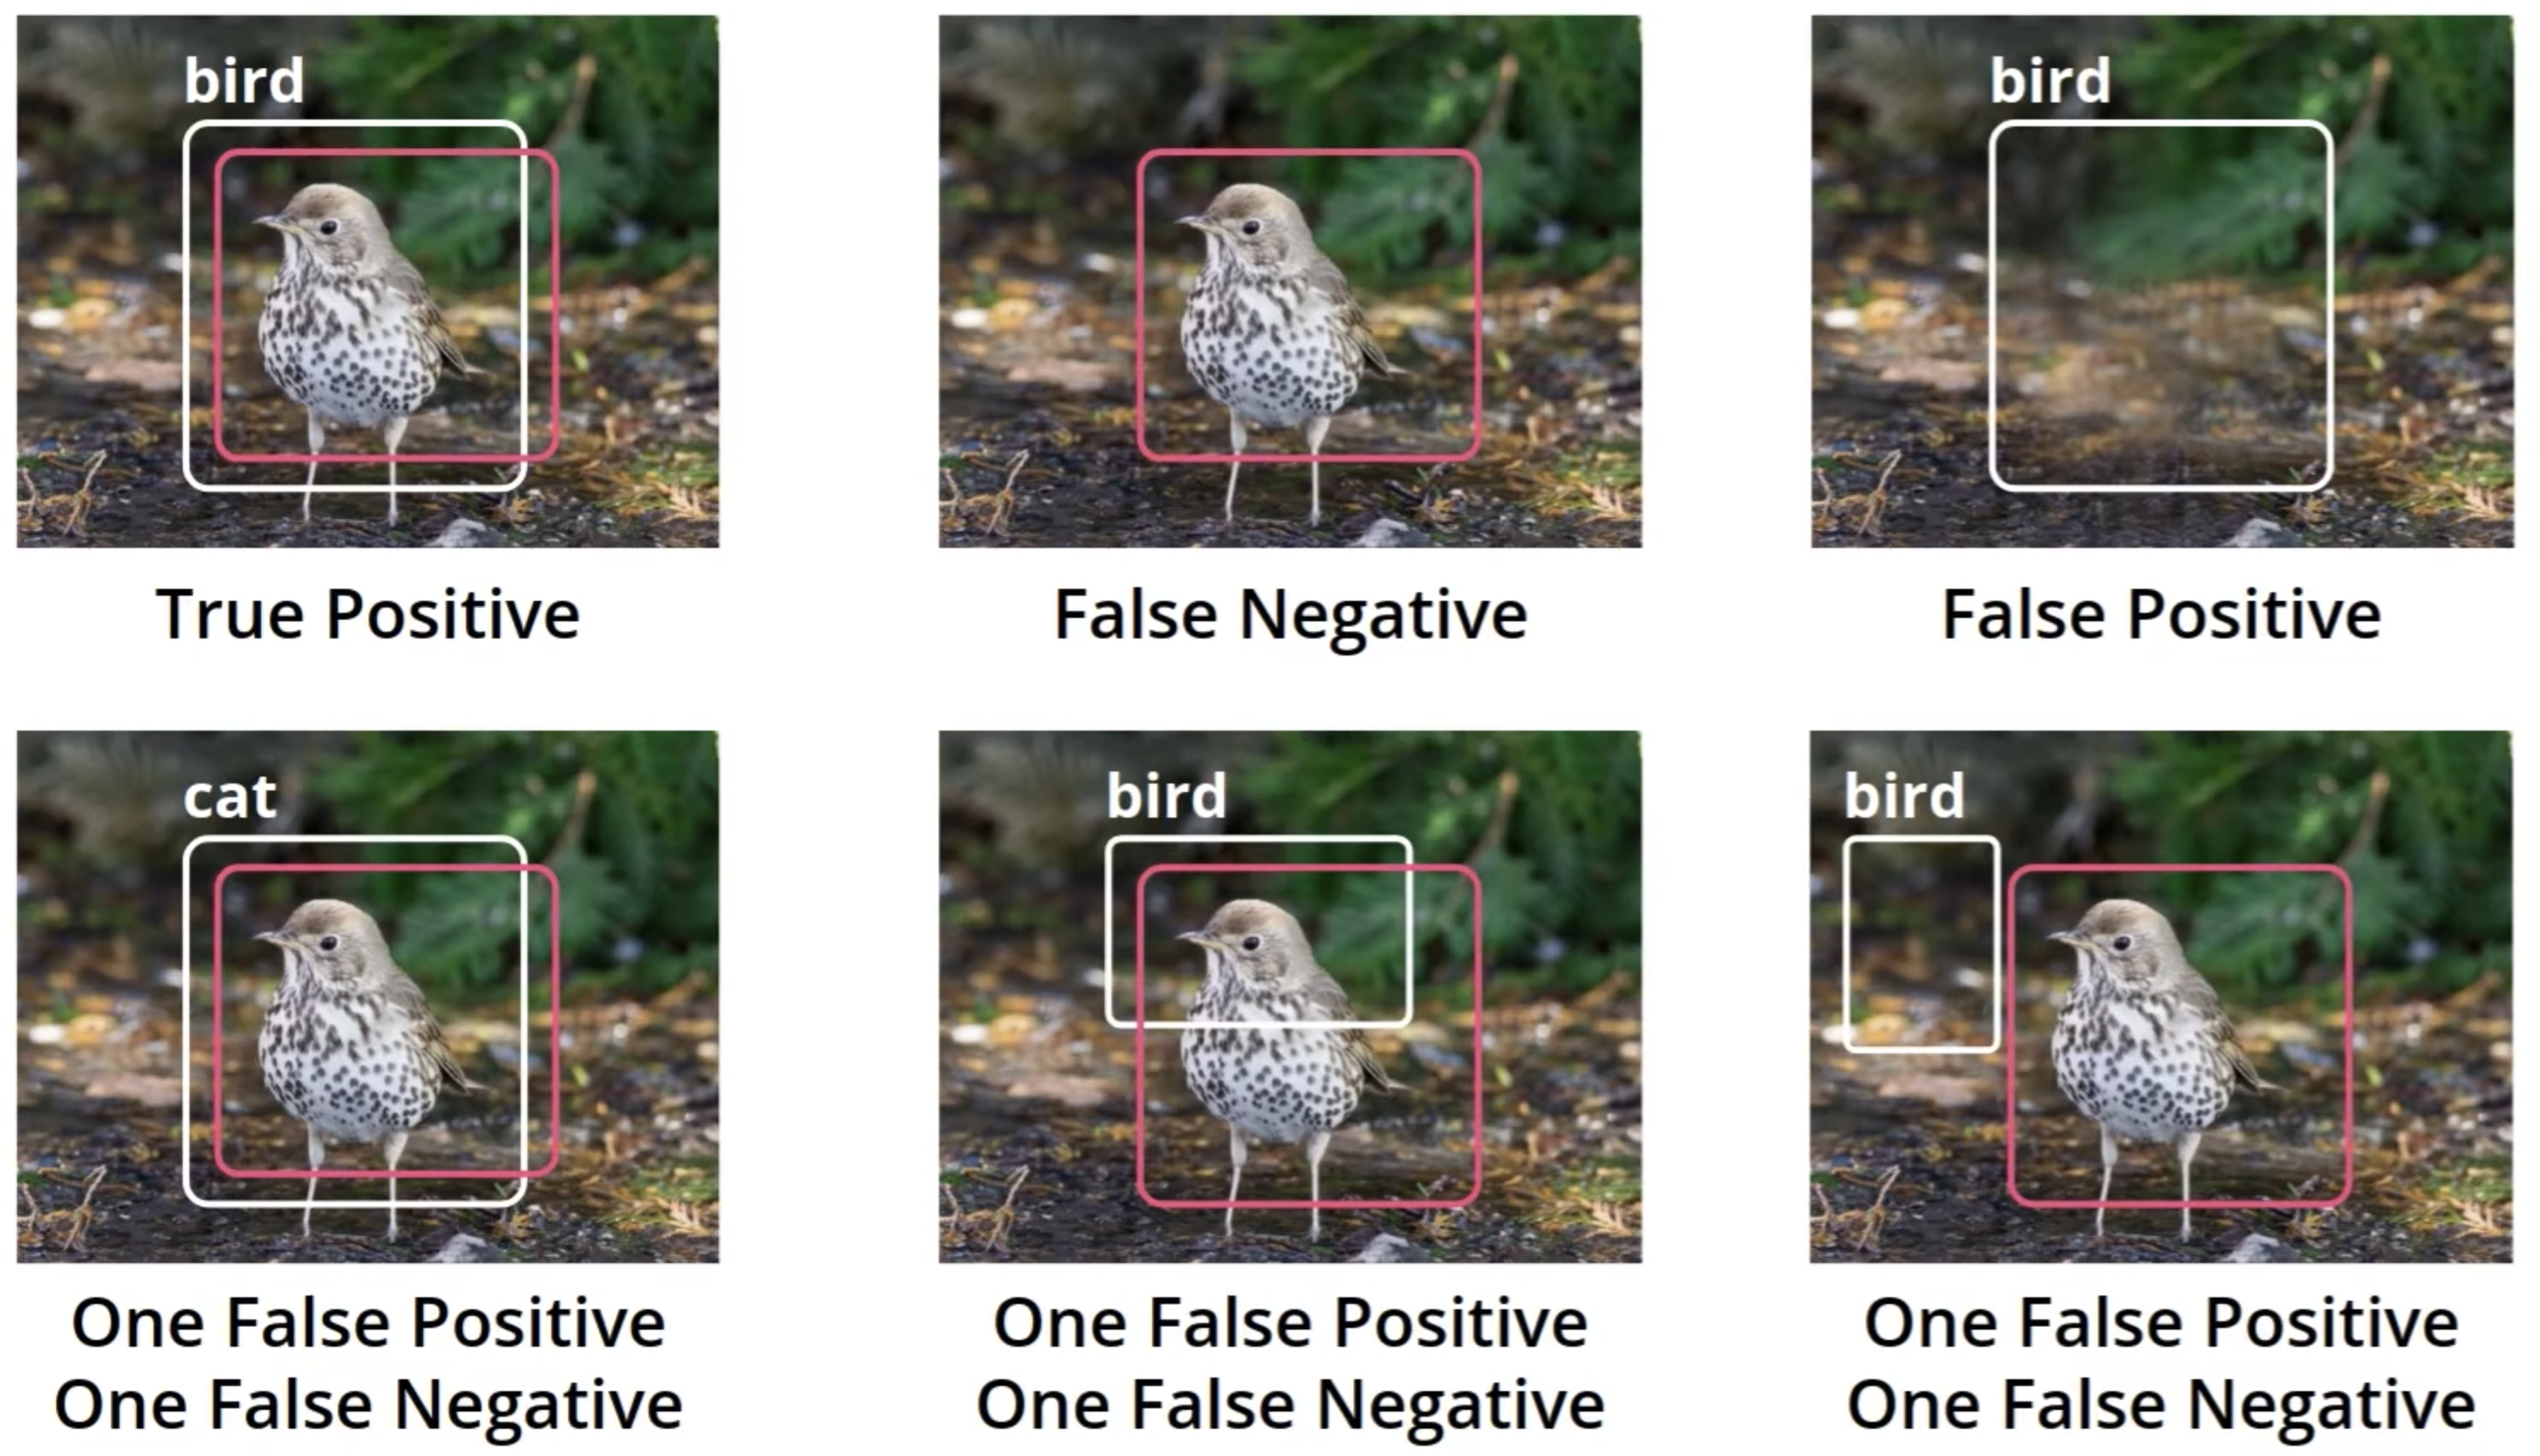
\includegraphics[width=0.75\linewidth]{img//intro/introNN/image.png}


\section{Perceptrons vs. Neural Networks}
Multilayer Perceptrons are Neural Networks. The perceptron and neural networks are inspired by biological neurons. Though modern "perceptrons" use the Logistic Sigmoid Function or other activation functions, classical perceptrons use a step function. \newline

Neural Networks are a more general class of models that encapsulates multi-layer perceptrons. Neural Networks are defined by having one or more hidden layers and an output layer that emits a decision -- either a predicted value, a probability, or a vector of probabilities, depending on the task.

\includegraphics[width=1\linewidth]{img//intro//introNN/screen-shot-2022-05-18-at-8.52.53-am.jpeg}

\section{Neural Network Architecture}
Ok, so we're ready to put these building blocks together, and build great Neural Networks! (Or Multi-Layer Perceptrons, however you prefer to call them.) \newline

Training a model to correctly classify non-linear data like that shown above requires superimposing multiple neural networks on top of one another.

\includegraphics[width=1\linewidth]{img//intro//introNN/neural-network-architecture-2.png}

We will combine two linear models to get our non-linear model. Essentially the steps to do this are:

\begin{itemize}
    \item Calculate the probability for each model
    \item Apply weights to the probabilities
    \item Add the weighted probabilities
    \item Apply the sigmoid function to the result
\end{itemize}

\includegraphics[width=1\linewidth]{img//intro//introNN/neural-network-architecture-3.png}

This calculation is run for every point in the plane.

\subsection{Weighting the Component Networks}
It is also possible to weight the input neural networks. For example, the model on the top left of the image below could be weighted more strongly than the model on the bottom left.

\includegraphics[width=1\linewidth]{img//intro//introNN/neural-network-architecture-4.png}

For example, the output of the top neural network could be given a weight of 7. The bottom could be given a weight of 5. An arbitrary bias of 6 could also be assigned.

\includegraphics[width=1\linewidth]{img//intro//introNN/neural-network-architecture-5.png}

Note that this exactly how neural networks themselves operate, except instead of \textbf{inputs to a neural network} we have \textbf{neural networks, themselves}.

\includegraphics[width=1\linewidth]{img//intro//introNN/neural-network-architecture-6.png}

By cleaning up and consolidating the network above, we arrive at the following.

\includegraphics[width=1\linewidth]{img//intro//introNN/neural-network-architecture-7.png}

Note that the following two networks are actually identical. One uses a notation where the bias (-6) is placed inside the node. The other uses a notation where the bias comes from a single node with constant input 1 where the edges are weighted by the bias. In both cases, the sigmoid activation function is used.

\includegraphics[width=1\linewidth]{img//intro//introNN/neural-network-architecture-8.png}

\subsection{Multiple layers}

Now, not all neural networks look like the one above. They can be way more complicated! Neural networks have a certain special architecture with layers:

\begin{itemize}
    \item The first layer is called the \textbf{input layer}, which contains the inputs.
    \item The next layer is called the \textbf{hidden layer}, which is the set of linear models created with the input layer.
    \item The final layer is called the \textbf{output layer}, which is where the linear models get combined to obtain a nonlinear model.
\end{itemize}

Neural networks can have different architectures, with varying numbers of nodes and layers:

\begin{itemize}
    \item \textbf{Input nodes.} In general, if we have \(n\) nodes in the input layer, then we are modeling data in n-dimensional space (e.g., 3 nodes in the input layer means we are modeling data in 3-dimensional space).
    \item \textbf{Output nodes.} If there are more nodes in the output layer, this simply means we have more outputs—for example, we may have a multiclass classification model.
    \item \textbf{Layers.} If there are more layers then we have a \textit{deep} neural network. Our linear models combine to create nonlinear models, which then combine to create even more nonlinear models!
\end{itemize}

\subsubsection{Adding More Nodes}
Adding more nodes to the hidden layer enables creation of more complex outputs, such as the triangular region shown below.

\includegraphics[width=1\linewidth]{img//intro//introNN/neural-network-architecture-10.png}

Adding more nodes to the \textbf{input layer} means the data space is higher dimensional. For example, in the network architecture below, the space is three-dimensional, the linear models in the hidden layers are planes, and the output layer bounds a nonlinear region in three space.

\includegraphics[width=1\linewidth]{img//intro//introNN/neural-network-architecture-11.png}

In general, if we have n dimensions in the input layer, we are living in n space. \newline

Adding more dimensions to the \textbf{output layer} means we have more outputs, and we are performing more complex, multiple-class classification.

\includegraphics[width=1\linewidth]{img//intro//introNN/neural-network-architecture-12.png}

\subsubsection{Adding More Layers}

If we add more layers, we have a \textbf{deep neural network}. Our nonlinear models combine to create even more nonlinear models.

\includegraphics[width=1\linewidth]{img//intro//introNN/neural-network-architecture-13.png}

This can be done many times, creating highly complex nonlinear models. Many of the models in real life, specifically, in applications such as self-driving cars and game-playing agents, have many hidden layers.

\includegraphics[width=1\linewidth]{img//intro//introNN/neural-network-architecture-14.png}

\subsection{Multi-Class Classification}
When we have three or more classes, we \textit{could} construct three separate neural networks—one for predicting each class. However, this is not necessary. Instead, we can add more nodes in the output layer. Each of these nodes will give us the probability that the item belongs to the given class.

\includegraphics[width=1\linewidth]{img//intro//introNN/neural-network-architecture-15.png}

When using neural networks to perform multi-class classification, the number of outputs must match the number of classifications. Then, we use the \lstinline|softmax| function on those outputs to obtain well-defined probabilities.

\subsection{Feedforward}
\href{https://www.youtube.com/watch?v=hVCuvMGOfyY&ab_channel=Udacity}{Youtube} \newline

\textbf{Feedforward} is the process neural networks use to turn the input into an output. In general terms, the process looks like this:

\begin{itemize}
    \item Take the input vector
    \item Apply a sequence of linear models and sigmoid functions
    \item Combine maps to create a highly non-linear map
\end{itemize}
As we saw in the video, the feedforward formula is: \[\hat{y} = \sigma \circ W^{(2)} \circ \sigma \circ W^{(1)}(x)\]

\subsubsection{Feedforward in Perceptrons}
Consider the example shown in the image below. The input is given by \(x = (x_1, x_2)\), and the label is \(y = 1\).

\includegraphics[width=1\linewidth]{img//intro//introNN/neural-network-architecture-16.png}

The perceptron receives the data point, \((x_1, x_2)\). The perceptron plots the point and outputs the probability that thte point is blue. Here, since the point is in the red area, the output would be a small number since the point is not very likely to be blue. But, in this case the point is blue, so the model does not appear to be very good.

\subsubsection{Feedforward in Neural Networks}
Feedforward operates in a similar manner for neural networks.

\includegraphics[width=1\linewidth]{img//intro//introNN/neural-network-architecture-17.png}

To discuss more specifically, introduce the following notation:
\begin{itemize}
    \item \(W^{(2)}\) - indicates the weight belongs to the second layer.
    \item \(W_{12}\) - indicates the weight is between the first node in the layer that is the input to the edge, and the second node in that layer that is the output to the edge.
\end{itemize}

\includegraphics[width=0.75\linewidth]{img//intro//introNN/neural-network-architecture-18.png}

The output prediction, \(\hat{y}\), is given by \[\hat{y} = \sigma \Bigg( \begin{matrix}W_{11}^{(2)} \\ W_{21}^{(2)} \\ W_{31}^{(2)}  \end{matrix} \Bigg) \sigma \Bigg( \begin{matrix}W_{11}^{(1)} & W_{12}^{(1)} \\ W_{21}^{(1)} & W_{22}^{(1)} \\ W_{31}^{(1)} & W_{32}^{(1)}  \end{matrix} \Bigg) \Bigg( \begin{matrix}x_1 \\ x_2 \\ 1 \end{matrix} \Bigg)\]

A more compact representation of the same equation is shown below. \[\hat{y} = \sigma \circ W^{(2)} \circ \sigma \circ W^{(1)}(x)\]

For a 3-layer neural network, like that shown below, the equation that follows would be used.

\includegraphics[width=0.75\linewidth]{img//intro//introNN/neural-network-architecture-19.png}

\[\hat{y} = \sigma \circ W^{(3)} \sigma \circ W^{(2)} \circ \sigma \circ W^{(1)}(x)\]

\subsection{Error Function}
\href{https://www.youtube.com/watch?v=SC1wEW7TtKs&ab_channel=Udacity}{Youtube} \newline

For a multilayer perceptron, as we saw, our prediction is simply a combination of matrix multiplications and sigmoid functions. But the error function can be the exact same formula, aside from the fact that \(\hat{y}\) is a bit more complicated. \[E(W) = -\frac{1}{m} \sum_{i=1}^m y_iln(\hat{y_i}) + (1-y_i) ln(1-\hat{y}_i)\]


\section{Exercise: Neural Network Architectures}

\subsubsection{Quiz Question}

Have a look at this code:
\begin{lstlisting}
class Net(nn.Module):
    def __init__(self):
        super().__init__()
        self.fc1 = Linear(1024, 128)
        self.fc2 = Linear(128, 64)
        self.fc3 = Linear(64, 1)

    def forward(self, x):
        x = relu(self.fc1(x))
        x = relu(self.fc2(x))
        x = sigmoid(self.fc3(x))
        return x
\end{lstlisting}
What does the line \verb|x = sigmoid(self.fc3(x))| do?
\begin{itemize}
    \item \textbf{Converts the output of \lstinline{self.fc3} to a probability between zero and one}
    \item Adds a layer to the neural network
    \item Computes the gradient of the input
    \item Combines the linear models in the hidden layer
\end{itemize}

\subsubsection{Quiz Question}

Assume you have the same code from question 1 above:
\begin{lstlisting}
class Net(nn.Module):
    def __init__(self):
        super().__init__()
        self.fc1 = Linear(1024, 128)
        self.fc2 = Linear(128, 64)
        self.fc3 = Linear(64, 1)

    def forward(self, x):
        x = relu(self.fc1(x))
        x = relu(self.fc2(x))
        x = sigmoid(self.fc3(x))
        return x
\end{lstlisting}
How would we modify this in a multi-class classification setting? \textit{(choose two)}
\begin{itemize}
    \item \textbf{Modify the number of output neurons in \lstinline{self.fc3}}
    \item Modify the size of the input in \lstinline{self.fc1}
    \item Change \lstinline{relu} to \lstinline{softmax}
    \item \textbf{Change \lstinline{sigmoid} to \lstinline{softmax}}
\end{itemize}


\subsubsection{Quiz Question}

Imagine you are developing a neural network that takes flattened 256 x 256 matrices as an input. Which of the following lines of code will work for your input layer?
\begin{itemize}
    \item \lstinline{self.fc1 = Linear(256, 128}
    \item \lstinline{self.fc1 = Linear(128, 256}
    \item This is the solution:\lstinline{self.fc1 = Linear(65536, 128}
    \item \lstinline{self.fc1 = Linear(128, 128}
\end{itemize}
Reasoning: Often, it's most readable to write our input layers for flattened m x n inputs as \verb|Linear(m * n, output_size)|.

\subsubsection{Quiz Question}

Imagine you are training your neural network but the accuracy is not improving -- you and your team determine that your model's decision boundary is not flexible enough to capture all the points. How could you improve your model? \textit{(Choose two)}
\begin{itemize}
    \item Increase the size of the input in the input layer
    \item \textbf{Increase the number of nodes in the hidden layers}
    \item Increase the size of  the output in the output layer
    \item \textbf{Add more layers to the model}
\end{itemize}

Reasoning: Although increasing the number of nodes in the hidden layers and adding layers to the model make it more complex, it often yields better performance.

\section{Activation Functions}
\href{https://www.youtube.com/watch?v=DhGm2clOS-U&ab_channel=Udacity}{Youtube}

\subsection{Activation Function Properties}

There are a wide variety of activation functions that we can use. Activation functions should be:

\begin{itemize}
    \item Nonlinear
    \item Differentiable, ideally continuously differentiable. That is, they have a derivative everywhere
    \item Monotonic: If you look at the function from left to right, the value on the y-axis never goes down.
    \item Close to the identity function at the origin
\end{itemize}
We can loosen these restrictions slightly. For example, ReLU is not differentiable at the origin. Others, like monotonicity, are very important and cannot be reasonably relaxed.

\includegraphics[width=1\linewidth]{img//intro//introNN/activation-functions.jpeg}

\paragraph{Rectified Linear Unit (ReLU)}

For many models, ReLU is the only activation function you'll see in the hidden neurons since it has great empirical performance and is easy to compute gradients on. ReLU is \textbf{not differentiable everywhere}: it is not differentiable at zero. 

\paragraph{Leaky ReLU}
Rather than zeroing out the output when it's negative, the Leaky ReLU ouputs one-tenth of the input.

\paragraph{Sigmoid}
Sigmoid bounds everything between 0 and 1. It also has easily computable derivatives. However, networks trained using sigmoid do not perform as well as those trained with ReLU. So it is rarely used in the hidden layers.

\paragraph{Hyperbolic tangent (tanh)}
Like sigmoid, tanh has the property of being bounded from above and below. Hence, all of the outputs are between -1 and +1. It is also centered at zero and has bigger derivatives than the sigmoid. 

\paragraph{Step function}

\paragraph{Gaussian Error linear units (GELU)}
GELU has been used in some transformer models, including Open AIs GPT-3.


\subsection{Quiz Question}
What factors can help you decide what activation function to use?

\textbf{Select all that apply.}

\begin{itemize}
    \item \textbf{Whether or not the activation function is bounded from above
    \item Whether or not the activation function is bounded from below
    \item The value of the activation function at the origin
    \item The ease of computing its gradient}
\end{itemize}

\section{Neural Network Objectives}
\href{https://www.youtube.com/watch?v=Q0u_THaU9n8&t=19s&ab_channel=Udacity}{Youtube} \newline

Once you know the output you're aiming for -- a binary classification, a classification into multiple classes, or a real number -- you can use that information to make decisions about your model.\newline

In particular, the combination of loss function and output activation function is dictated by the type of problem that you have.

\includegraphics[width=1\linewidth]{img//intro//introNN/image2.png}

\textbf{Binary Classification:}
\begin{itemize}
    \item Target: Something that can be encoded to one or zero. E.g. whether the image is a cat or not
    \item Output layer: Sigmoid activation function
    \item Loss function we want to minimize is the binary cross-entropy
\end{itemize}

\textbf{Multiclass Classification:}
\begin{itemize}
    \item More than one class for classifiation
    \item  Target: Vector of possible targets with the length of the vector being the number of classes. The numerical value of  that class is the position in the vector. 

    \includegraphics[width=0.5\linewidth]{img//intro//introNN/image3.png}
    
    \item The output probability vector will have values distributed across those classes. The most probable class will be the one with the highest probability.
\end{itemize}

\textbf{Regression:}
\begin{itemize}
    \item Activation function: Identity or bounded (so we do not get negative values with something like ReLU)
    \item Error functions: Mean Squared Error or Mean Absolute Error
\end{itemize}

\section{Decision Boundaries}
\href{https://www.youtube.com/watch?v=aPgH8Ra30T0&ab_channel=Udacity}{Youtube} \newline

Our data will dictate what the shape of our decision boundary should be. Neural networks will be able to find decision boundaries that are high-dimensional and nonlinear by combining the decision boundaries of the hidden neurons. Even in cases where we cannot visualize our decision boundary easily, knowing the approximate complexity of our decision boundary will inform how big our model needs to be. 

\subsection{Linear Decision Boundaries}
\includegraphics[width=0.25\linewidth]{img//intro//introNN/image4.png}
\begin{itemize}
    \item simplest kinds of decision bounds
    \item Straight line that best divides the data
    \item Binary classes and two dimensions
    \item Rarely want to use neural networks
\end{itemize}

\subsection{Higher Dimensional Decision Boundaries}
\includegraphics[width=0.25\linewidth]{img//intro//introNN/image5.png}
\begin{itemize}
    \item Divide classes with a hyperplane
    \item Given \(n\) variables, output \(n - 1\) dimensional hyperplane
    \item Cannot visualize hyperplanes in dimension greater than 3
    \item Still linear and not common for neural networks
\end{itemize}

\subsection{Nonlinear Decision Boundaries}
\includegraphics[width=0.25\linewidth]{img//intro//introNN/image6.png}
\begin{itemize}
    \item High-dimensional, non-linear hyperplanes are common in neural networks
    \item Since each neuron is introducing some hyperplane and we are aggregating the hyperplanes of these various neurons, these hyperplanes can be 100+ dimensions
    \item Nearly impossible to visualize decision boundaries. Can sometimes try to visualize with t-SNE
    \item Complex data = complex decision boundary
    \item Complex decision boundary = big neural network
\end{itemize}


\section{Quiz Question}

Look at the following code snippet, an example of the classic \href{https://en.wikipedia.org/wiki/LeNet}{\textbf{LeNet-5}} model:
\begin{lstlisting}
class Net(nn.Module):
    def __init__(self):
        super().__init__()
        self.conv1 = nn.Conv2d(3, 6, 5)
        self.pool = nn.MaxPool2d(2, 2)
        self.conv2 = nn.Conv2d(6, 16, 5)
        self.fc1 = nn.Linear(16  *5*  5, 120)
        self.fc2 = nn.Linear(120, 84)
        self.fc3 = nn.Linear(84, 10)

    def forward(self, x):
        x = self.pool(F.relu(self.conv1(x)))
        x = self.pool(F.relu(self.conv2(x)))
        x = torch.flatten(x, 1) 
        x = F.relu(self.fc1(x))
        x = F.relu(self.fc2(x))
        x = self.fc3(x)
        return x
\end{lstlisting}
How would you need to modify it for the road hazard detection system, assuming we are using \href{https://pytorch.org/docs/stable/generated/torch.nn.BCELoss.html\#torch.nn.BCELoss}{\textbf{\lstinline{nn.BCELoss}}} as our loss function?

(Select all that apply.)
\begin{itemize}
    \item Add more hidden layers
    \item \textbf{Change the size of the output layer}
    \item \textbf{Add an activation function to the output layer}
    \item Change the \lstinline{Linear} layers to \lstinline{Conv2d} layers
\end{itemize}

Answer: The output layer should have a single sigmoid-activated neuron that gives us a probability that there is a hazard in the road.


\section{Glossary}

For your reference, here are all the new terms we introduced in this lesson:

\begin{itemize}
    \item \textbf{Neural Networks} are defined by having one or more hidden layers and an output layer that emits a decision -- either a predicted value, a probability, or a vector of probabilities, depending on the task.
    \item \textbf{Neural Networks Layers:}

\begin{itemize}
        \item The first layer is called the \textbf{input layer}, which contains the inputs.
        \item The next layer is called the \textbf{hidden layer}, which is the set of linear models created with the input layer.
        \item The final layer is called the \textbf{output layer}, which is where the linear models get combined to obtain a nonlinear model.
\end{itemize}

    \item \textbf{Neural Network Nodes:}

\begin{itemize}
        \item \textbf{Input nodes.} In general, if we have\textit{n} nodes in the input layer, then we are modeling data in n-dimensional space (e.g., 3 nodes in the input layer means we are modeling data in 3-dimensional space).
        \item \textbf{Output nodes.} If there are more nodes in the output layer, this simply means we have more outputs—for example, we may have a multiclass classification model.
        \item \textbf{Layers.} If there are more layers then we have a \textit{deep} neural network. Our linear models combine to create nonlinear models, which then combine to create even more nonlinear models!
\end{itemize}

    \item \textbf{Feedforward} is the process neural networks use to turn the input into an output.
\end{itemize}

\chapter{Training Neural Networks}

\section{What We'll Learn}

Having a conceptual framework for neural networks is important, but so is actually training the models. In this lesson, we will learn how to:

\begin{itemize}
    \item Distinguish between underfitting and overfitting
    \item Visualize our training with TensorBoard
    \item Optimize the training process with early stopping, regularization, dropout, random restarts, learning rate decay, and momentum
    \item Use PyTorch to build and train a neural network
\end{itemize}

\section{Training, Validation, and Testing}
\href{https://www.youtube.com/watch?v=HWt6gu5f3Q4&ab_channel=Udacity}{Youtube}\newline

\begin{itemize}
    \item Divide data to provide more information
    \begin{itemize}
        \item \textbf{Training}: Data actually used to fit model
        \item \textbf{Validation}: Data used during training to evaluate generalization. The validation dataset provides a lot of influence on the model since it informs how the model is likely to performs on the test data. This means it is a good leading indication for whether or not we have a problem with our data.
        \item Test: Data used to evaluate final model. Test data should be completely separated from the training and validation datasets. 
    \end{itemize}
\end{itemize}

\subsection{Dividing Data}

We typically divide our data into three sets whose size can vary, but a good rule of thumb is the 80/10/10 rule:

\begin{itemize}
    \item Train (80\%)
    \item Validation (10\%)
    \item Test (10\%)
\end{itemize}
Another powerful approach is k-fold cross-validation, where the data is split up into some number, which we call k, equal parts. One is used as the validation set, one is used as the test set, and the remaining parts are used as the training set. We then cycle through all combinations of the data until all parts have had a chance to be the test set.

\section{Overfitting and Underfitting}
\href{https://www.youtube.com/watch?v=xj4PlXMsN-Y&ab_channel=Udacity}{Youtube} \newline

When we train our models, it is entirely possible to get them to a point where they perform very well on our training data—but then perform very poorly on our testing data. Two common reasons for this are \textbf{underfitting} and \textbf{overfitting}

\subsection{Underfitting}

\begin{itemize}
    \item Underfitting means that our model is too simplistic. There is a poor fit between our model and the data because we have \textbf{oversimplified} the problem.
    \item Underfitting is sometimes referred to as \textbf{error due to bias}. Our training data may be biased and this bias may be incorporated into the model in a way that oversimplifies it.
\end{itemize}
For example, suppose we train an image classifier to recognize dogs. And suppose that the only type of animal in the training set is a dog. Perhaps the model learns a biased and overly simple rule like, "if it has four legs it is a dog". When we then test our model on some data that has other animals, it may misclassify a cat as a dog—in other words, it will \textit{underfit} the data because it has \textit{error due to bias}.

\subsection{Overfitting}

\begin{itemize}
    \item Overfitting means that our model is too complicated. The fit between our model and the training data is \textbf{too specific}—the model will perform very well on the training data but will \textbf{fail to generalize} to new data.
    \item Overfitting is sometimes referred to as \textbf{error due to variance}. This means that there are random or irrelevant differences among the data points in our training data and we have fit the model so closely to these irrelevant differences that it performs poorly when we try to use it with our testing data.
\end{itemize}
For example, suppose we want our image classifier to recognize dogs, but instead we train it to recognize "dogs that are yellow, orange, or grey." If our testing set includes a dog that is brown, for example, our model will put it in a separate class, which was not what we wanted. Our model is too specific—we have fit the data to some unimportant differences in the training data and now it will fail to generalize.

\subsection{Applying This to Neural Networks}

Generally speaking, underfitting tends to happen with neural networks that have overly simple architecture, while overfitting tends to happen with models that are highly complex.

\includegraphics[width=0.75\linewidth]{img//intro//trainingNN/training-considerations-3.png}

The bad news is, it's really hard to find the right architecture for a neural network. There is a tendency to create a network that either has overly simplistic architecture or overly complicated architecture. In general terms, the approach we will take is to err on the side of an overly complicated model, and then we'll apply certain techniques to reduce the risk of overfitting.

\includegraphics[width=0.75\linewidth]{img//intro//trainingNN/image.png}

\section{Early Stopping}
\href{https://www.youtube.com/watch?v=NnS0FJyVcDQ&t=2s&ab_channel=Udacity}{Youtube} \newline

When training our neural network, we start with random weights in the first epoch and then change these weights as we go through additional epochs. Initially, we expect these changes to improve our model as the neural network fits the training data more closely. But after some time, further changes will start to result in overfitting.

\includegraphics[width=1\linewidth]{img//intro//trainingNN/training-considerations-4.png}

We can monitor this by measuring both the \textbf{training error} and the \textbf{testing error}. As we train the network, the training error will go down—but at some point, the testing error will start to increase. This indicates overfitting and is a signal that we should stop training the network prior to that point. We can see this relationship in a \textbf{model complexity graph} like this one:

\includegraphics[width=1\linewidth]{img//intro//trainingNN/training-considerations-5.png}

\includegraphics[width=1\linewidth]{img//intro//trainingNN/early-stopping.png}
\captionof{figure}{Model complexity graph}

Have a look at the graph and make sure you can recognize the following:

\begin{itemize}
    \item On the Y-axis, we have a measure of the error and on the X-axis we have a measure of the complexity of the model (in this case, it's the number of epochs).
    \item On the left we have high testing and training error, so we're underfitting.
    \item On the right, we have high testing error and low training error, so we're overfitting.
    \item Somewhere in the middle, we have our happy Goldilocks point (the point that is "just right").
\end{itemize}
In summary, we do gradient descent until the testing error stops decreasing and starts to increase. At that moment, we stop. This algorithm is called \textbf{early stopping} and is widely used to train neural networks.


\section{Visualizing Training with Tensorboard}
\href{https://www.youtube.com/watch?v=MKoW6vUYStk&t=1s&ab_channel=Udacity}{Youtube} \newline

After launching Tensorboard from the command line and choosing a directory for the logs, we use the \verb|SummaryWriter| class from \verb|torch.utils.tensorboard|. Using the \verb|add_scalar| method, we can write things like loss and accuracy. We can also put images and figures into Tensorboard using \verb|add_image| and \verb|add_figure| respectively. \newline

For further information, check the \href{https://pytorch.org/docs/stable/tensorboard.html}{\textbf{PyTorch Tensorboard documentation}}

\section{Regularization}
\href{https://www.youtube.com/watch?v=KxROxcRsHL8&ab_channel=Udacity}{Youtube} \newline

Consider a situation where we are attempting to split two points, and have two possible models that could be used. We are trying to find the model with the smallest error.

\includegraphics[width=0.75\linewidth]{img//intro//trainingNN/image2.png}

A couple of reminders:
\begin{itemize}
    \item The prediction is: \(\hat{y} = \sigma(w_1 x_1 + w_2 x_2 + b)\)
    \item The general equation for a linear model is: \(w_1 x_1 + w_2 x_2 + b = 0\)
\end{itemize}

\textbf{Solution 1}: \(x_1 + x_2\)\newline
Notice that the bias \(b\) is \(0\) and \(w_1\) and \(w_2\) are both equal to \(1\).
\begin{itemize}
    \item \(\sigma(1 + 1) = 0.88\)
    \item \(\sigma(-1 + -1) = 0.12\)
\end{itemize}

\textbf{Solution 2}: \(10x_1 + 10x_2\)
\begin{itemize}
    \item \(\sigma(10 + 10) = 0.9999...\)
    \item \(\sigma(-10 + -10) = 0.000000...2\)
\end{itemize}

\textbf{Solution}: \(10x_1 + 10x_2\). The error is smaller if the prediction is closer to the actual label. Great intuition about the error function! \href{https://www.youtube.com/watch?v=ndYnUrx8xvs&t=66s&ab_channel=Udacity}{Youtube}\newline

But, the model is overfit in a subtle way. The sigmoid functions for the two models are shown in \ref{fig:activationFunc} and as shown, the second solution is too certain and its sigmoid function is too steep. As a result, it is much harder to do gradient descent since the derivatives are mostly close to 0, except where it crosses the y-axis and becomes very large. It is difficult to train under these circumstances. Hence, we would prefer to have a model as on the left.

\includegraphics[width=1\linewidth]{img//intro//trainingNN/actibation-functions.png}
\captionof{figure}{Activation functions}
\label{fig:activationFunc}


\begin{itemize}
    \item When we apply sigmoid to small values such as \(x_1 + x_2\), we get the function on the left, which has a nice slope for gradient descent.
    \item When we multiply the linear function by 10 and take sigmoid of \(10 x_1 + 10 x_2\), our predictions are much better since they're closer to zero and one. But the function becomes much steeper and it's much harder to do gradient descent.
\end{itemize}
Conceptually, the model on the right is too certain and it gives little room for applying gradient descent. Also, the points that are classified incorrectly in the model on the right will generate large errors and it will be hard to tune the model to correct them. \newline

Now the question is, how do we prevent this type of overfitting from happening? The trouble is that large coefficients are leading to overfitting, so what we need to do is adjust our error function by, essentially, penalizing large weights. \newline

If you recall, our original error function looks like this: \[-\frac{1}{m} \sum_{i = 1}^m (1 - y_i) \ln{(1 - \hat{y}_i)} + y_i \ln{(\hat{y}_i)}\]
We want to take this and add a term that is big when the weights are big. There are two ways to do this. One way is to add the sums of absolute values of the weights times a constant lambda: \[+ \lambda(|w_i| + ... + |w_n|)\]

The other one is to add the sum of the squares of the weights times that same constant: \[+ \lambda (w_1^2 + ... + w_n^2)\]

In both cases, these terms are large if the weights are large.

\includegraphics[width=1\linewidth]{img//intro//trainingNN/training-considerations-9.png}

\subsection{L1 vs L2 Regularization}

The first approach (using absolute values) is called \textbf{L1 regularization}, while the second (using squares) is called \textbf{L2 regularization}. Here are some general guidelines for deciding between the two:

\subsubsection{L1 Regularization}

\begin{itemize}
    \item L1 tends to result in sparse vectors. That means small weights will tend to go to zero.
    \item If we want to reduce the number of weights and end up with a small set, we can use L1.
    \item L1 is also good for feature selection. Sometimes we have a problem with hundreds of features, and L1 regularization will help us select which ones are important, turning the rest into zeroes.
\end{itemize}

\subsubsection{L2 Regularization}

\begin{itemize}
    \item L2 tends not to favor sparse vectors since it tries to maintain all the weights homogeneously small.
    \item L2 gives better results for training models so it's the one we'll use the most.
\end{itemize}

\includegraphics[width=0.75\linewidth]{img//intro//trainingNN/training-considerations-10.png}

\section{Implementing Regularization}\label{implementing-regularization}

In this exercise, you will implement both L1 and L2 regularization from
scratch in NumPy. In PyTorch, L2 regularization is typically handled in
the optimizer, via the \lstinline!weight\_decay!
parameter, but we will also implement a manual L1 and L2 loss penalty in
PyTorch.

\begin{lstlisting}[language=Python]
# DO NOT EDIT THIS CELL
import numpy as np
import torch
from torch import nn
from torch import optim
import torch.nn.functional as F
from torch.utils.data import DataLoader
from torchvision import transforms
from torchvision import datasets
import matplotlib.pyplot as plt
\end{lstlisting}

\subsection{L1 Regularization -- Numpy}\label{l1-regularization-numpy}

L1 regularization is the sum of the absolute values of the weights times
a scaling constant, lambda. Below, you will define the function
\lstinline!l1\_regularization! that accepts an input
vector and a scalar constant, lambda.

\textbf{NOTE:} We use the variable name \lstinline!lamb!
rather than \lstinline!lambda! since
\lstinline!lambda! is a keyword in Python.

\begin{lstlisting}[language=Python]
def l1_regularization(weights, lamb):
    absolute_weights = np.abs(weights)
    return lamb * np.sum(absolute_weights)
\end{lstlisting}

\begin{lstlisting}[language=Python]
# Grading code. Run this cell to test your code!
grading_vector = np.array([1, -2, 3, -4])
assert l1_regularization(grading_vector, 0.5) == 5, f"Your L1 regularization implementation seems to be incorrect. Expected 5, got {l1_regularization(grading_vector, 0.5)}"
assert l1_regularization(grading_vector, 1) == 10, f"Your L1 regularization implementation seems to be incorrect. Expected 10, got {l1_regularization(grading_vector, 1)}"

print("Great work!")
\end{lstlisting}

\begin{lstlisting}
Great work!
\end{lstlisting}

\subsection{L2 Regularization -- Numpy}\label{l2-regularization-numpy}

L2 regularization squares the weights inside the vector and returns the
sum of those squares times a scaling constant, lambda. Below, you will
define the function \lstinline!l2\_regularization!, which
accepts an input vector and a scalar constant, lambda.

\begin{lstlisting}[language=Python]
def l2_regularization(weights, lamb):
    squared_weights = np.dot(weights, weights.T)
    return lamb * squared_weights
\end{lstlisting}

\begin{lstlisting}[language=Python]
# Grading code. Run this cell to test your code!
grading_vector = np.array([0.5, -1, 1.5, -2])
assert l2_regularization(grading_vector, 0.5) == 3.75, f"Your L2 regularization implementation seems to be incorrect. Expected 3.75, got {l2_regularization(grading_vector, 0.5)}"
assert l2_regularization(grading_vector, 1) == 7.5, f"Your L2 regularization implementation seems to be incorrect. Expected 7.5, got {l2_regularization(grading_vector, 1)}"

print("Great work!")
\end{lstlisting}

\begin{lstlisting}
Great work!
\end{lstlisting}

\subsection{Regularization in PyTorch}\label{regularization-in-pytorch}

Although L2 regularization is typically handled via the
\lstinline!weight\_decay! parameter in your optimizer, we
can compute L1 and L2 regularization by hand. We do this by iterating
over the parameters in our model using the
\lstinline!net.parameters()! method.

Rather than establishing a model, training it, and testing it, we will
manually set the model weights.

\begin{lstlisting}[language=Python]
# Setting up our net for testing
net = nn.Sequential(nn.Linear(4, 1, bias=False))
# Make it so autograd doesn't track our changes
with torch.no_grad():
    net[0].weight = nn.Parameter(torch.ones_like(net[0].weight))
    net[0].weight.fill_(2.0)
\end{lstlisting}

\begin{lstlisting}[language=Python]
# Define L1 loss
def l1_torch(model, lamb):
    return lamb * sum([p.abs().sum() for p in model.parameters()])

# Define L2 loss
def l2_torch(model, lamb):
    return lamb * sum([(p**2).sum() for p in model.parameters()])
\end{lstlisting}

\begin{lstlisting}[language=Python]
# Grading code
assert l1_torch(net, 1) == 8, f"There is something wrong with your L1 regularization implementation. Expected 8, got {l1_torch(net, 1)}"
assert l1_torch(net, 0.5) == 4, f"There is something wrong with your L1 regularization implementation. Expected 4, got {l1_torch(net, 0.5)}"

assert l2_torch(net, 1) == 16, f"There is something wrong with your L2 regularization implementation. Expected 16, got {l2_torch(net, 1)}"
assert l2_torch(net, 0.25) == 4, f"There is something wrong with your L2 regularization implementation. Expected 4, got {l2_torch(net, 0.25)}"

print("Great work!")
\end{lstlisting}

\begin{lstlisting}
Great work!
\end{lstlisting}

\begin{lstlisting}[language=Python]
\end{lstlisting}



\section{Dropout}
\href{https://www.youtube.com/watch?v=Ty6K6YiGdBs&ab_channel=Udacity}{Youtube} \newline

When training a neural network, sometimes one part of the network has very large weights and it ends up dominating the training, while another part of the network doesn't really play much of a role (so it doesn't get trained).

To solve this, we can use a method called \textbf{dropout} in which we turn part of the network off and let the rest of the network train:

\begin{itemize}
    \item We go through the epochs and randomly turn off some of the nodes. This forces the other nodes to pick up the slack and take a larger part in the training.
    \item To drop nodes, we give the algorithm a parameter that indicates the probability that each node will get dropped during each epoch. For example, if we set this parameter to 0.2, this means that during each epoch, each node has a 20\% probability of being turned off.
    \item Note that some nodes may get turned off more than others and some may never get turned off. This is OK since we're doing it over and over; on average, each node will get approximately the same treatment.
\end{itemize}

\section{Local Minima and Random Restart}
\href{https://www.youtube.com/watch?v=gF_sW_nY-xw&t=1s&ab_channel=Udacity}{Youtube} \newline
Gradient descent looks at the direction where it can most decrease the error and then it takes a step in that direction. However, if there are multiple low points in the solution space, gradient descent may end up leading us to \textbf{local minima}—solutions where the error is at the lowest point in the local area, but not the lowest point overall.

\includegraphics[width=0.75\linewidth]{img//intro//trainingNN/training-considerations-13.png}

One way to solve our problem is to use \textbf{random restart}. We start (and restart) from a few different random places and do gradient descend from all of them. This increases the probability that we'll get to the global minimum, or at least a pretty good local minimum. 

\includegraphics[width=0.75\linewidth]{img//intro//trainingNN/training-considerations-15.png}

\href{https://www.youtube.com/watch?v=idyBBCzXiqg&t=1s&ab_channel=Udacity}{Youtube on random restart}


\section{Exercise: Training Techniques}

\subsection{Scenario 1:}

You are training a neural network and see the following accuracy and loss in TensorBoard:

\includegraphics[width=1\linewidth]{img//intro//trainingNN/screen-shot-2022-04-10-at-7.01.14-am.jpeg}

Based on the screenshot, what is happening to your model?

(Select all that apply.)

\begin{itemize}
    \item It is underfitting to the training set
    \item \textbf{It is overfitting to the training set}
    \item \textbf{It is stuck in a local minimum}
    \item It has not trained long enough
\end{itemize}
Solution: This model has gotten stuck in a local minimum very quickly and vastly overfit the training set.

Which \textbf{two} of the following techniques would be most helpful for this scenario?
\begin{itemize}
    \item Training for more epochs
    \item \textbf{Early stopping}
    \item \textbf{Random restart}
    \item Dropout
\end{itemize}
Solution: Early stopping will help us with our overfitting problem and random restart can help us escape the local minimum.


\subsection{Scenario 2:}

You're training another neural network and find the following accuracy and loss in TensorBoard:

\includegraphics[width=1\linewidth]{img//intro//trainingNN/screen-shot-2022-04-10-at-7.44.41-am.jpeg}

Which of the following is occurring?
\begin{itemize}
    \item \textbf{The model is not sufficiently trained}
    \item The model is underfit to the training set
    \item The model is overfit to the training set
    \item The model is stuck in a local minimum
\end{itemize}
Solution: Looking carefully also shows that our learning rate is probably too low. Underfitting and undertraining can look very similar, but underfitting means that the model is too simple, not that it hasn't trained long enough. We can see that the loss is still decreasing at a similar rate each epoch -- it hasn't leveled off.

\section{Vanishing and Exploding Gradients}
\href{https://www.youtube.com/watch?v=ff3GFgnE4PU&t=62s&ab_channel=Udacity}{Youtube} \newline

\subsection{Vanishing gradients}
\textbf{Vanishing gradients} are common for certain activation function with limited range. These are also called \textbf{"saturating" activation functions}. This means that as error back backpropagates through the model, the error signal becomes weaker. Ths is more common in deeper neural networks. 

We have our output neuron which gives our loss. We then compute that error and backpropagate the error through the network. The input to the output neuron is going to consist of the input from the prior hidden layer. So the relative contribution to the neuron highlighted in blue (right after the output error on the right side of \autoref{fig:vanishingGradient2}) is the product of the partial derivative of the loss with respect to the weight of the blue neuron, and the error signal sent back to that is going to be a little smaller than the overall signal since it is split between the inputs. 

\includegraphics[width=0.75\linewidth]{img//intro//trainingNN/image2.png}
\captionof{figure}{ }
\label{fig:vanishingGradient2}

Because of how backpropagation works via the chain rule, the error sent to the neuron in the last hidden layer is that partial derivative with respect to the weight of the neuron and the prior layer. And this is again going to be a bit smaller. 

\includegraphics[width=1\linewidth]{img//intro//trainingNN/image3.png}

This signal has to travel all the way back through the network. So if the gradient is relatively small to begin with, we are multiplying progressively smaller numbers between \(0\) and \(1\) by each other, causing our gradient to completely vanish by the time it reaches the earliest layers. 

This problem can be solved by using non-saturating activation functions like ReLU.  However, function like ReLu contribute e to different problems: the \textbf{exploding gradients}.

\subsection{Exploding gradients}
The exploding gradients are more common in deeper networks as there are more opportunities for these gradients to be multiplied against each other. These are common for non-saturating activation functions like ReLU. These function are unbounded so their gradients can easily be greater than \(1\).  \newline

We want to backpropagate the error through the model. Assuming the gradient of the error with respect to that top neuron is reasonably sized, but greater than \(1\). Then the gradient with respect to each preceding layer is going to be the product of all the preceding gradients. So if the gradients are larger than one (for these non-saturating activation functions, they can be significantly larger than \(1\)), the gradient will grow exponentially larger and can \textbf{explode}. \newline

This causes instability and makes it hard to train a model. 
\subsection{How to know}
Watch weights of neurons on TensorBoard. \newline

Vanishing gradient: Weights of neurons drop to 0 but loss is relatively high but stalled. \newline

Exploding gradient: Neuron weights become very large during training. Loss is unstable. It can jump significantly from epoch to epoch and possibly even going to NaN.

\includegraphics[width=0.75\linewidth]{image.png}

To solve either of them, consider changing the activation function.  For exploding gradients, consider gradient clipping or weight regularization.

\subsection{Quiz Question}

Consider the six activation functions depicted above. Which of the six are most susceptible to \textit{vanishing} gradients?

*\textit{Select all that apply}

\begin{itemize}
    \item ReLU
    \item Leaky ReLu
    \item \textbf{Sigmoid}
    \item \textbf{tanh}
    \item \textbf{Step}
    \item GELU

\end{itemize}


\subsection{Quiz Question}

In addition to changing the activation function, we can use the \href{https://pytorch.org/docs/stable/generated/torch.nn.utils.clip_grad_norm_.html}{\textbf{\lstinline{torch.nn.utils.clip_grad_norm_}}} function to clip our gradients. What effect will this have?
\begin{itemize}
    \item \textbf{Prevent exploding gradients by bound the norm of the gradient}
    \item Prevent vanishing gradients by adding noise to the gradient
    \item Prevent exploding gradients by bounding the value of the gradient
    \item PRevent vanishing gradients by setting a minimum gradient size
\end{itemize}
Solution: We can also use the \href{https://pytorch.org/docs/stable/generated/torch.clamp.html#torch.clamp}{\textbf{\lstinline{clamp}}} method to restrict the minimum and maximum size of our tensors.

\section{Learning Rate Decay}
\href{https://www.youtube.com/watch?v=TwJ8aSZoh2U&ab_channel=Udacity}{Youtube} \newline

Here are some key ideas to keep in mind when choosing a \textbf{learning rate}:

If the learning rate is \textbf{large}:

\begin{itemize}
    \item This means the algorithm is taking large steps, which can make it faster.
    \item However, the large steps may cause it to miss (overshoot) the minimum.
\end{itemize}
If the learning learning rate is \textbf{small}:

\begin{itemize}
    \item This means the algorithm is taking small steps, which can make it slower.
    \item However, it will make steady progress and have a better chance of arriving at the local minimum.
\end{itemize}
If your model is not working, a good general rule of thumb is to try decreasing the learning rate. The best learning rates are those that decrease as the algorithm is getting closer to a solution.

\includegraphics[width=1\linewidth]{img//intro//trainingNN/training-considerations-26.png}

\section{Momentum}
\href{https://www.youtube.com/watch?v=r-rYz_PEWC8&t=1s&ab_channel=Udacity}{Youtube} \newline
 
Another way to solve the local minimum problem is with \textbf{momentum}. In the analogy, this would mean walking quickly and with momentum to “power through” small increases in the error function, so that a lower minimum can be found. Momentum is a constant \(\beta\) between \(0\) and \(1\). \newline

We use \(\beta\) to get a sort of weighted average of the previous steps: \[{step}(n) + \beta {step}(n - 1) + \beta^2{step}(n) + \beta^3{step}(n - 2) + ...\]

\includegraphics[width=1\linewidth]{img//intro//trainingNN/image4.png}

The previous step gets multiplied by \(1\), the one before it gets multiplied by \(\beta\), the one before that by \(\beta^2\), the one before that by \(\beta^3\), and so on. Because \(\beta\) has a value between \(0\) and \(1\), raising it to increasingly large powers means that the value will get smaller and smaller. In this way, the steps that happened a long time ago will be multiplied by tiny values and thus matter less than the ones that happened recently.\newline

This can get us over "humps" and help us discover better minima. Once we get to the global minimum, the momentum will still be pushing us away, but not as much.


\section{Optimizers}
\href{https://www.youtube.com/watch?v=4Ocl-2lwO6U&t=1s&ab_channel=Udacity}{Youtube} \newline

We want to change weight to minimize error. Gradient descent is an optimization algorithm that works for many but not all problems since it does not incorporate things like learning rate or momentum. One of the most common optimizers for NN is Adaptive Moment Estimation (Adam).  \newline

With Adam, the learning rate does not vanish and it quickly converges to a minimum.  

\subsection{Choosing an Optimizer}

Our choice of optimizer is not often the most important decision in training a model, but it can definitely make a difference. While Adam is a good default, the use of SGD is still common. The various optimizers available in PyTorch are covered in \href{https://pytorch.org/docs/stable/optim.html}{\textbf{the \lstinline{torch.optim} documentation}}

\subsection{Quiz Question}

What parameter of the Adam optimizer tells it how big of a step to take when we call the \verb|.step()| method?

You can reference \href{https://pytorch.org/docs/stable/generated/torch.optim.Adam.html\#torch.optim.Adam}{\textbf{the documentation}} if you get stuck.
\begin{itemize}
    \item \lstinline{params}
    \item \textbf{\lstinline{lr}}
    \item \lstinline{betas}
    \item \lstinline{weight_decay}
\end{itemize}
Solution: The learning rate is a very important parameter for our optimizer. If we set it too small, training may not converge. Setting the learning rate too high can cause the optimizer to overshoot the global minimum.

\section{Batch vs Stochastic Gradient Descent}
\href{https://www.youtube.com/watch?v=2p58rVgqsgo&t=1s&ab_channel=Udacity}{Youtube}
\subsection{Batch Gradient Descent}

First, let's review our \textbf{batch gradient descent} algorithm:

\begin{itemize}
    \item In order to decrease error, we take a bunch of steps following the negative of the gradient, which is the error function.
    \item Each step is called an \textit{epoch}.
    \item In each epoch, we take our input (all of our data) and run it through the entire neural network.
    \item Then we find our predictions and calculate the error (how far the predictions are from the actual labels).
    \item Finally, we back-propagate this error in order to update the weights in the neural network. This will give us a better boundary for predicting our data.
\end{itemize}
If we have a large number of data points then this process will involve huge matrix computations, which would use a lot of memory.

\subsection{Stochastic Gradient Descent}

To expedite this, we can use only \textit{some} of our data at each step. If the data is well-distributed then a subset of the data can give us enough information about the gradient.

This is the idea behind \textbf{stochastic gradient descent}. We take small subsets of the data and run them through the neural network, calculating the gradient of the error function based on these points and moving one step in that direction.

We still want to use all our data, so what we do is the following:

\begin{itemize}
    \item Split the data into several batches.
    \item Take the points in the first batch and run them through the neural network.
    \item Calculate the error and its gradient.
    \item Back-propagate to update the weights (which will define a better boundary region).
    \item Repeat the above steps for the rest of the batches.
\end{itemize}
Notice that with this approach we take multiple steps, whereas with batch gradient descent we take only one step with all the data. Each step may be less accurate, but, in practice, it's much better to take a bunch of slightly inaccurate steps than to take only one good one.


\section{Training Techniques in PyTorch}
\href{https://www.youtube.com/watch?v=dmeeuBWa1us&t=1s&ab_channel=Udacity}{Youtube} \newline

When using PyTorch without API, early stopping has to be implemented by programmer. 

\subsection{Implementing Training Techniques in PyTorch}

The various training optimizations we've covered are relatively easy to implement when training our networks. Though early stopping is not written into PyTorch itself, implementing it in the training loop is fairly easy.

Our other techniques are more straightforward and can be found in the PyTorch documentation:

\begin{itemize}
    \item \href{https://pytorch.org/docs/stable/generated/torch.nn.Dropout.html}{\textbf{Dropout}}
    \item Momentum and learning rate decay are implemented in the \href{https://pytorch.org/docs/stable/optim.html}{\textbf{optimizer}}
\end{itemize}

\subsection{Writing Training Loops}
\href{https://www.youtube.com/watch?v=Ek3_IL-kt6Y&ab_channel=Udacity}{Youtube} 

To write a training loop, one typically begins with the \verb|for epoch in range(epochs)| syntax. Then, loading each batch from the dataloader, the steps of training are:

\begin{itemize}
    \item Zeroing out the optimizer's gradients with \verb|optimizer.zero_grad()|
    \item Computing the outputs with \verb|net(inputs)|
    \item Computing the loss with \verb|criterion(outputs, labels)|
    \item Computing the gradient of the loss with \verb|loss.backward()|
    \item Taking an update step with the optimizer using \verb|optimizer.step()|
\end{itemize}
We can also implement early stopping, compute validation loss and accuracy, and print updates in the training loop.

\section{Lesson Review}
At the beginning of this lesson, we needed to develop the skills to actually train a neural network using PyTorch. In this lesson, we learned how to:

\begin{itemize}
    \item Split our data into training, validation, and test sets
    \item Distinguish between and understand the causes of underfitting and overfitting
    \item Optimize the model training process with early stopping, regularization, and dropout
    \item Define a loss function and optimizer to train a neural network
    \item Write a training loop to use PyTorch to build a neural network
\end{itemize}
Using these skills, we can train a neural network from scratch and ensure that it generalizes well to unseen data.

\section{Glossary}

For your reference, here are all the new terms we introduced in this lesson:

\begin{itemize}
    \item \textbf{Training Data}: Data actually used to fit the model
    \item \textbf{Validation Data}: Data used during training to evaluate generalization
    \item \textbf{Test Data:} Data used to evaluate the final model
    \item \textbf{Underfitting} (also called error due to bias): Underfitting means that our model is too simplistic because of a poor fit between our model, and the data because we have oversimplified the problem.
    \item \textbf{Overfitting} (also called error due to variance)\textbf{:} Overfitting means that our model is too complicated, and the fit between our model and the training data is too specific—the model will perform very well on the training data but will fail to generalize to new data.
    \item \textbf{Early Stopping:} Implementing gradient descent until the testing error stops decreasing and starts to increase.
    \item \textbf{Dropout}: The process of turning part of the network off and letting the rest of the network train
    \item \textbf{Local Minima:} solutions where the error is at the lowest point in the local area, but not the lowest point overall.
    \item \textbf{Momentum:} Momentum is a constant \(\beta\) between 00 and 11.
    \item \textbf{Stochastic gradient descent}: The process of taking small subsets of the data and running them through the neural network, calculating the gradient of the error function based on these points, and moving one step in that direction.
\end{itemize}

\part{Convolutional Neural Networks}
\chapter{Introduction to CNNs}
\href{https://www.youtube.com/watch?v=-dLdeL6BAZs&t=1s&ab_channel=Udacity}{Youtube} \newline

A CNN is a neural network developed specifically for image and video processing. CNNs are used to automate many tasks, for example:

\begin{itemize}
    \item Image classification
    \item Object recognition
    \item Anomaly detection
    \item Image captioning
\end{itemize}
... and many others. They are widely used across many industries, including medicine, banking, manufacturing, insurance, real-estate, transportation (self-driving cars), and social networks.\newline

CNNs are arguably the main technology responsible for the Artificial Intelligence renaissance we are witnessing today, with billion of dollars in revenue generated by their application.\newline

We are very excited for you to be here with us and to learn about this invaluable technology!


\section{Course Overview}

\begin{itemize}
    \item Introduction to CNNs and basic concepts

\begin{itemize}
        \item Use Multi-Layer Perceptrons (MLPs) for image classification
        \item Understand the limitations of MLPs for images and how CNNs overcome them
        \item Learn basic concepts of CNNs and what makes them so powerful for image tasks
\end{itemize}

    \item CNNs in more depth

\begin{itemize}
        \item Learn all the basic layers that make up a CNN
        \item Put all the basic layers together to build a CNN from scratch
        \item Classify images using CNNs
        \item Use various methods to improve CNN performance
        \item Export models for production
\end{itemize}

    \item Transfer learning

\begin{itemize}
        \item Understand key innovative CNN architectures
        \item Implement transfer learning using a pre-trained network to classify different sets of images
        \item Fine-tune a pre-trained network on a new dataset
\end{itemize}

    \item Autoencoders

\begin{itemize}
        \item Explain the functionality of autoencoders for data compression, image denoising, and dimensionality reduction
        \item Build a simple autoencoder out of linear layers to perform anomaly detection
        \item Build CNN autoencoders to perform anomaly detection and image denoising
\end{itemize}

    \item Object detection and segmentation

\begin{itemize}
        \item Describe object detection, object localization, and image segmentation.
        \item Train and evaluate a one-stage object detection model to detect multiple objects in an image.
        \item Train and evaluate a semantic segmentation model to classify every pixel of an image.
\end{itemize}

\end{itemize}


\section{Prerequisites}

\subsection{Who Should Take This Course}

This course is intended for a student who is at least somewhat familiar with the basic concepts of elementary neural networks, and has good experience with Python programming.

\subsection{What You Should Already Know}

\subsubsection{Python}

\begin{itemize}
    \item Variables
    \item Loops
    \item Conditionals
    \item Functions
    \item \href{https://realpython.com/python3-object-oriented-programming/}{\textbf{Object-Oriented Programming, Classes}}
\end{itemize}
Experience with the Python scientific stack (NumPy, Matplotlib...) is going to be useful.

For the class we will be extensively using \href{https://tacc.github.io/CSC2017Institute/docs/day1/jupyter.html}{\textbf{Jupyter Notebooks}}.

\subsubsection{Machine Learning}

\begin{itemize}
    \item \href{https://machinelearningmastery.com/gradient-descent-for-machine-learning/}{\textbf{Loss function and gradient descent}}
    \item Train / validation / test split
    \item \href{https://machinelearningmastery.com/neural-networks-crash-course/}{\textbf{Neural Networks}}: We will recap these basic concepts, but some previous understanding of these concepts is required:

\begin{itemize}
        \item Perceptrons and Multi-Layer Perceptrons (MLP)
        \item Activations and functions (ReLU, softmax…)
        \item Training a neural network
        \item Overfitting and underfitting
        \item Forward pass, backpropagation
        \item Regularization and \href{https://machinelearningmastery.com/dropout-for-regularizing-deep-neural-networks/}{\textbf{DropOut}}
\end{itemize}

\end{itemize}

\subsubsection{PyTorch}

We will briefly review all these concepts, but some previous familiarity with them will be helpful:

\begin{itemize}
    \item Datasets and dataloaders
    \item Common loss functions
    \item Training, validation, and test loops
    \item Multi-Layer Perceptrons in PyTorch
\end{itemize}

\section{Business Stakeholders}
\href{https://www.youtube.com/watch?v=JrCeIxzb2Fs&ab_channel=Udacity}{Youtube} \newline

If you use CNNs to power a real product in a real-world setting, you are going to interact with several different profiles:

\begin{itemize}
    \item Data Scientist / Machine Learning Engineer: Responsible for developing the ML pipeline and the model, as well as performing all the relevant analytics - for example on data quality and performance measurements.
    \item Data Engineers: Responsible for the data ingestion pipelines, the quality of the data that the DS/MLE receive, and for provisioning the right data at inference time.
    \item Software Engineers: Responsible for the production environment, both front-end and back-end, as well as for many pieces of the MLOps infrastructure. Involve them from the beginning to make sure that the model you are producing can fit into the production environment.
    \item DevOps Engineers: Help in handling the infrastructure, including training servers, various MLOps tools, and other infrastructure needed to train and deploy a model.
    \item Product Managers: Define the right problem to solve, exploit the knowledge of the customers, and define quantifiable deliverables and success criteria for the project. The PM also helps in keeping the project on time and on budget.
    \item Customers: Consumer of the product; we should always consider the customers' and users' perspectives for every decision that we make.
\end{itemize}

\section{History of CNNs}
\href{https://www.youtube.com/watch?v=1J6SM_3FoY4&ab_channel=Udacity}{Youtube} \newline

A brief history of CNNs:

\begin{itemize}
    \item \href{https://news.cornell.edu/stories/2019/09/professors-perceptron-paved-way-ai-60-years-too-soon}{\textbf{Perceptron (1958)}}: A one-neuron primitive neural network capable of classifying linearly-separable datasets.
    \item \href{https://en.wikipedia.org/wiki/Neocognitron\#:~:text=The\%20neocognitron\%20is\%20a\%20hierarchical,inspiration\%20for\%20convolutional\%20neural\%20networks.}{\textbf{Neocognitron (1980)}}: A neural network using two types of mechanisms that are the basis of modern CNNs: convolution and pooling.
    \item \href{https://en.wikipedia.org/wiki/Backpropagation\#History}{\textbf{Backpropagation (1986)}}: Allows training of neural networks end to end based on data.
    \item \href{https://en.wikipedia.org/wiki/Multilayer_perceptron}{\textbf{Multi-Layer Perceptron (1986)}}: The first proper neural network in the modern sense, theoretically capable of modeling any function.
    \item \href{http://yann.lecun.com/exdb/lenet/}{\textbf{LeNet-5 (1998)}}: The first proper Convolutional Neural Network with practical application, used to model handwritten digits obtaining an accuracy of almost 99\%. This seminal work sparked a new renaissance of work on Convolutional Neural Networks for image recognition.
    \item \href{https://qz.com/1034972/the-data-that-changed-the-direction-of-ai-research-and-possibly-the-world/}{\textbf{ImageNet (2010-2017)}}: A competition with the goal of modeling with the largest possible accuracy a large dataset of more than 1 million natural images classified into 1000 classes.
\end{itemize}
The ImageNet competition spawned several innovations, starting with AlexNet, the first CNN to win the contest. AlexNet won in 2012 by a huge margin, when the runners-up were still trying to use classical computer vision methods. After 2012, every team in the competition used Convolutional Neural Networks.

Since then, the performance on the ImageNet dataset has continued improving at a very fast pace. Most of the architectures from around 2012 - 2020 were based exclusively on Convolutional Neural Networks. After that, a different class of neural network called Transformers started to conquer the top of the rankings. These days the most accurate architectures such as ViT and CoAtNet use a mix of CNN and Transformer elements. Many of these architectures also use additional data.

CNNs however are still the workhorses for real-world applications of neural networks on images, because they can achieve very good performances while requiring orders of magnitude less data and compute than pure Transformers.

\section{Tools \& Environment}
\href{https://www.youtube.com/watch?v=qV-o9eVOWTs&ab_channel=Udacity}{Youtube} \newline
All the software that you need to complete the exercises and develop your final project is pre-installed in the Udacity workspaces here in your classroom.\newline

If you want to run something locally, every exercise and the project come with a file (\verb|requirements.txt|) which contains all the dependencies that you need to install. You can install them in your Python environment by issuing the command: \verb|pip install -r requirements.txt|.\newline

In many cases you will need a GPU to complete the exercises and the project with reasonable execution times. The Udacity workspace we provide in your classroom comes with a GPU that you can opt to use. If instead you want to run locally, you will need to install all the relevant software needed for your GPU to work with PyTorch. You can find some instructions \href{https://pytorch.org/get-started/locally/}{\textbf{here}}.\newline

\section{Project Preview}
\href{https://www.youtube.com/watch?v=4R5eOA7hCuA&t=3s&ab_channel=Udacity}{Youtube} \newline

n the final project, you will classify landmarks in images uploaded to a social network, in order to localize the images. \newline

You will be given the dataset containing the images and their label (the landmark contained in the image). You will train two CNNs: one that you will design from scratch, and a standard one that you will fine-tune on the dataset. You will also build a little app, powered by your best model.

\chapter{CNN Conecepts}

\section{Lesson Outline}
\href{https://www.youtube.com/watch?v=zS4iCL3lDtU&ab_channel=Udacity}{Youtube} \newline

In this lesson we are going to learn the general concepts underlying Convolutional Neural Networks (CNNs), and how they relate to the neural networks you already know, Multi-layer Perceptrons (MLPs).\newline

We will start by applying MLPs to the images of a very famous computer vision dataset, then see the limitations of MLPs when it comes to images.\newline

We'll then learn how Convolutional Neural Networks solve these limitations, allowing them to outperform MLPs for all image tasks.\newline

Finally, we will introduce at a high level the conceptual underpinnings of CNNs that make them so powerful and useful.

\section{MNIST Dataset}
\href{https://www.youtube.com/watch?v=a7bvIGZpcnk&t=1s&ab_channel=Udacity}{Youtube} 

\subsection{Image Classification and the MNIST Dataset}

Classifying an image means assigning one label to the entire image. The label could be for example the most prominent object in the image ("cat," "dog,"...), or a characteristic of the image ("cloudy sky," "sunny sky,"...).

The MNIST database is arguably the most famous dataset in the field of deep learning. It contains 70,000 handwritten digits 0-9 in white over a black background, and the task is to classify each image by assigning it the label corresponding to the depicted number.

It is nowadays considered a solved problem, with modern neural networks having performances that are on par or better than human performances and over 99.9\% accurate. However, it is still widely used for tutorials and in the literature as the first, most obvious benchmark for new ideas.

\section{How Computers Interpret Images}
\href{https://www.youtube.com/watch?v=mEPfoM68Fx4&t=2s&ab_channel=Udacity}{Youtube} \newline

\subsection{Definitions}

Before continuing, let's define some of the terms that we are going to use:

\begin{itemize}
    \item \textbf{Vector} - an array of numbers with only one dimension
    \item \textbf{Matrix} - an array of numbers with two dimensions
    \item \textbf{Array} or tensor - two interchangeable generic terms which can mean arrays with one, two, or n dimensions
\end{itemize}

\subsection{Computer Interpretation of Images}

An image is seen by the computer as an array of values (a matrix). A grid of values for each grid cell is called a pixel, and each pixel has a numerical value.

\includegraphics[width=0.5\linewidth]{img//cnn/image.png}

The images in the MNIST dataset are 28 x 28 and 8-bit grayscale. This means that the computer represents each one of them as a square matrix of 28 x 28 elements, where the value in the element of the matrix represents the light intensity with a range of 0 to 255: 0 means pure black and 255 means pure white.

\includegraphics[width=0.1\linewidth]{img//cnn/image2.png}


\subsection{Normalizing Image Inputs}

Data normalization is an important pre-processing step for neural networks. The activation functions that are normally used in neural networks (sigmoid, ReLU, etc.,...) have the highest rate of change around 0:

\includegraphics[width=1\linewidth]{img//cnn/image3.png}

This means that their derivative is large for inputs that are not too far from 0. Since we train neural networks with gradient descent, the training can proceed faster if the weights stay in the vicinity of where the activation function changes rapidly, i.e., close to 0. \newline

The weights of a neural network are typically initialized with a mean of 0, i.e., some weights are negative and some are positive, but they are in general between -1 and +1, close to 0. Remember that these weights are multiplied with the feature values (in this case the pixel values) and then a bias is added on top before the result is fed to the activation function. \newline

Therefore, if we want the input of the activation function to be somewhere close to 0, we need to start with a number that is close to zero, because two numbers close to zero multiplied together give another number close to zero. \newline

So we need to take the pixels in the input image, which in the case of a grayscale image have values between 0 and 255, and renormalize them to be close to zero. \newline

The easiest way is to just divide the value by 255, thereby changing the pixel values to be between 0 and 1.

\includegraphics[width=1\linewidth]{img//cnn/image-normalized.png}

In many cases, we go further than that: we compute the mean and the standard deviation of all the pixels in the renormalized dataset, then we subtract the mean and divide by the standard deviation for each image separately. Therefore, our transformed data will contain both negative and positive pixels with mean 0 and standard deviation 1. Sometimes you'll see an approximation here, where we use a mean and standard deviation of 0.5 to center the pixel values. If you'd like, you can \href{https://pytorch.org/docs/stable/}{\textbf{read more here about the Normalize transformation in PyTorch.}}


\subsection{Classification with Neural Networks}

We already know how to perform classification with neural networks, and in particular with a Multi-Layer Perceptron (MLP). This network takes as input a grayscale image (a matrix) and outputs a vector of scores or a vector of probabilities (one for each class). The class corresponding to the maximum of that vector corresponds to the best guess for the label of the image.

\subsection{Flattening}

Suppose we want to use an MLP to classify our image. The problem is, the network takes a 1d array as input, while we have images that are 28x28 matrices. The obvious solution is to \textit{flatten} the matrix, i.e., to stack all the rows of the matrix in one long 1d vector, as in the image below.

\includegraphics[width=0.75\linewidth]{img//cnn/flattening-bw.jpeg}
\captionof{figure}{To flatten an image we take the rows and stack them together in a 1d array}
\label{img:flattening}

Using the example of \autoref{img:flattening} with a 4x4 image, we have a matrix with 16 pixel values. Instead of representing this as a 4x4 matrix, we can construct a vector with 16 entries where the first 4 entries of our vector correspond to the first row of our old array,The second 4 entries correspond to the second row, and so on. After converting our images into vectors. they can then be fed into the input layer of an MLP. 

\section{MLP Structure and Class Scores}

\subsection{MLP for Images}
\href{https://www.youtube.com/watch?v=4zFq5U1IHgU&ab_channel=Udacity}{Youtube} \newline


\subsection{A Multi-Layer Perceptron for MNIST}
The input of our MLP must obviously be 28 x 28=784, which corresponds to the dimension of the flattened image. The output of the MLP must also be obviously a vector with 10 elements (one for each class). The values in this vector are proportional to the probability that the network assigns to each class. So if the network thinks that it is most likely that the given image is an 8, then the element in the array corresponding with 8 should be the largest. The output values are also called class scores. Class scores indicate how sure the network is that a given input is of a specific class. The class scores are often represented as a vector of values or even as a bar graph, indicating the relative strengths of the scores. \newline

But what goes between the input and the output? How many hidden layers, and how many neurons?

\includegraphics[width=0.75\linewidth]{img//cnn/mlp.jpeg}
\captionof{figure}{Schematic of a Possible MLP for the Classification of Images in the MNIST Dataset}


\section{Loss and Optimization}
\href{https://www.youtube.com/watch?v=583E6aKwQig&ab_channel=Udacity}{Youtube} \newline

\begin{itemize}
    \item Loss: Measure any mistakes between a predicted and true class
    \item Backpropagation: We can compute the gradient of the loss with respect to the models weights. This way quantify how bad a particular weight is in making a mistake
    \item Optimization: we can choose an optimization function like gradient descent to give us a way to calculate a better weight value.
\end{itemize}

\includegraphics[width=1\linewidth]{img//cnn/image5.png}

We need to make the output layer more interpretable. We apply a \textbf{softmax} activation function to convert these scores into probabilities. \newline

As a model trains, its goal will be to find the weights that minimize this loss function,and therefore it gives us the most accurate predictions. A \textbf{loss function and backpropagation} give us a way to quantify how bad a particular network weight is based on how close a predicted and a true class label are from one another. \newline

Next, we need a way to calculate a better weight value. Think of the loss function as a surface that resembles a mountain range. Then to minimize this function, we need only find a way to descend to the lowest valley. This is the role of an optimizer, the standard method for minimizing the loss and optimizing for the best weight values is called gradient descent. \newline

\subsection{Loss Function}

The \textbf{loss function} quantifies how far we are from the ideal state where the network does not make any mistakes and has perfect confidence in its answers.

Depending on the task and other considerations we might pick different loss functions. For image classification the most typical loss function is the \textbf{Categorical Cross-Entropy (CCE) loss}, defined as: \[CCE = -\sum_{i=1}^{n_{classes}} y_i \log \hat{p}_i\]
where:

\begin{itemize}
    \item The sum is taken over the classes (10 in our case)
    \item yi is the ground truth, i.e., a \href{https://en.wikipedia.org/wiki/One-hot\#Machine_learning_and_statistics}{\textbf{one-hot encoded vector}} of length 10
    \item pi is the probability predicted by the network
\end{itemize}

\begin{quote}
NOTE: In PyTorch it is customary to have the network output class scores (or \textit{logits}) instead of probabilities like in other frameworks. Then, the PyTorch loss function itself will first normalize the scores with a Softmax function, and then compute the CCE loss.

\end{quote}

\includegraphics[width=0.5\linewidth]{img//cnn/image4.png}

\subsection{Gradient Descent}

The values of the weights and the biases in the MLP are optimized by using Gradient Descent (or more precisely Stochastic Gradient Descent or SGD for short), or similar algorithms such as \href{https://optimization.cbe.cornell.edu/index.php?title=Adam}{\textbf{Adam}}. SGD takes the derivative of the loss with respect to the weights and then updates the values of the weights so as to decrease the loss as quickly as possible.

\section{Loading Data and Transforming Images in PyTorch}

\subsection{Loading Images in PyTorch}

\subsubsection{Transforms}

Before we can feed images to a neural network, there are some operations we must perform. As we have seen before, we need to normalize the images so the values in the pixels are floating point numbers between 0 and 1, or -1 and 1, instead of values from 0 to 255 as in the RGB format. We also need to transform them to PyTorch Tensors, so our network can handle them. \newline

In many cases we also want to augment our dataset by performing random transformations, but more on this in a later lesson. \newline

For the moment, let's see how to normalize the images and transform them to tensors:
\begin{lstlisting}
import torchvision.transforms as T

## T.Compose creates a pipeline where the provided
## transformations are run in sequence
transforms = T.Compose(
    [

        # This transforms takes a np.array or a PIL image of integers
        # in the range 0-255 and transforms it to a float tensor in the
        # range 0.0 - 1.0
        T.ToTensor(),

        # This then renormalizes the tensor to be between -1.0 and 1.0,
        # which is a better range for modern activation functions like
        # Relu
        T.Normalize((0.5), (0.5)),
    ]
)
\end{lstlisting}
In many real-world datasets we also need some other operations like resizing, which we will see later.

\subsubsection{Datasets}

PyTorch offers dataset and dataloaders specific for images and their annotations.\newline

A \verb|Dataset| instance provides methods to load and manipulate the data, whereas a \verb|DataLoader| instance wraps the dataset and allows iterations over it during training, validation, and test. \newline

It is possible to define custom datasets when needed, but the \verb|torchvision| library offers specific classes inheriting from the base \verb|Dataset| class for all major computer vision datasets. You can find a list of these datasets \href{https://pytorch.org/vision/stable/datasets.html\#image-classification}{\textbf{here}}. For example, you can load the MNIST dataset just by doing:
\begin{lstlisting}
train_data = datasets.MNIST(
    root="data", train=True, download=True, transform=transforms
)

test_data = datasets.MNIST(
    root="data", train=False, download=True, transform=transforms
)
\end{lstlisting}
\verb|torchvision| also offers an \verb|ImageFolder| class that can be used to extract images and labels directly from a local directory.

You have to structure your data in the following way:

\includegraphics[width=0.5\linewidth]{img//cnn/imagefolder.jpeg}

We need a top-level directory with the name of your dataset (\verb|custom_data| in this case). Then, we need one or more subdirectories representing the classes. In this case we have a dataset of cats and dogs, and accordingly we have two subdirectories with the same name. Within each subdirectory we place the images belonging to that class. \newline

The \verb|ImageFolder| dataset class can auto-probe the classes (by using the names of the subdirectories) and can assign each image to the right class by looking into which subdirectory the image is placed. \newline

This is how to use the \verb|ImageFolder| class:
\begin{lstlisting}
from torchvision import datasets

train_data = datasets.ImageFolder(
  "/data/custom_data",
  transform=transforms
)
\end{lstlisting}
\subsubsection{Dataloaders}

A \textbf{dataloader} allows sequential or random iterations over a dataset or over a subset of a dataset.\newline

For example, a dataloader for MNIST can be obtained as follows:
\begin{lstlisting}
train_data = datasets.MNIST(
    root="data", train=True, download=True, transform=transforms
)

train_loader = torch.utils.data.DataLoader(
  dataset=train_data, 
  shuffle=True, 
  batch_size=batch_size,
  num_workers=num_workers
)
\end{lstlisting}
The parameter \verb|batch_size| indicates the size of the mini-batch for Stochastic Gradient Descent, while \verb|num_workers| indicates the number of processes that PyTorch should use to load the data. It is important to be able to feed the GPU with enough data to keep it busy, otherwise the training will be slow. By using several processes that are reading data in parallel, PyTorch can increase the GPU usage and the speed of training. A good rule of thumb is to use a number of workers equal to the number of CPUs on the current machine:

\begin{lstlisting}
import multiprocessing

n_workers = multiprocessing.cpu_count()
\end{lstlisting}

Once you have a dataloader, you can easily loop over all the data one batch at a time:

\begin{lstlisting}
for image_batch, label_batch in train_loader:
    ... do something ...
\end{lstlisting}

If all you want to do is obtain the next batch, then:

\begin{lstlisting}
## Get an iterator from the dataloader
dataiter = iter(train_loader)
## Get the next batch
image_batch, label_batch = dataiter.next()
\end{lstlisting}

\paragraph{Splitting Train and Validation Data}

It is typical to extract a validation set from the training data, for things like hyperparameter optimization and to prevent overfitting by monitoring the relationship between train and validation loss. We also reserve a test set for testing after the model development has finished. \newline

It is easy to split a dataset using PyTorch:

\begin{lstlisting}
## Let's keep 80% of the training data for training
train_len = int(len(trainval_data) * 0.8)

## Let's use the remaining for validation
val_len = len(trainval_data) - train_len

## Perform a random split of the train dataset
train_subset, val_subset = torch.utils.data.random_split(
    trainval_data, [train_len, val_len]
)

## Now we can use the subsets as normal datasets
train_loader = torch.utils.data.DataLoader(
    dataset=train_subset, shuffle=True, batch_size=batch_size, num_workers=num_workers
)

val_loader = torch.utils.data.DataLoader(
    dataset=val_subset, shuffle=False, batch_size=batch_size, num_workers=num_workers
)
\end{lstlisting}
\section{Defining a Network in PyTorch}
\href{https://www.youtube.com/watch?v=nM-J4eAb-pI&t=1s&ab_channel=Udacity}{Youtube} \newline

\subsection{Recap of the Structure of a Neural Network in PyTorch}

A model in PyTorch is implemented as a class with at least two methods: the \verb|__init__| method and the \verb|forward| method. \newline

The \verb|__init__| method should initialize all the layers that the model uses, while the \verb|forward| method implements a forward pass through the network (i.e., it applies all the layers to the input). Note that the backward pass for backpropagation is executed by PyTorch \href{https://pytorch.org/tutorials/beginner/blitz/autograd_tutorial.html}{\textbf{automatically}} and does not need to be implemented. \newline

So a typical model in PyTorch looks like this:
\begin{lstlisting}
import torch
import torch.nn as nn

class MyModel(nn.Module):

  def __init__(self):

    super().__init__()

    # Create layers. In this case just a standard MLP
    self.fc1 = nn.Linear(20, 10)
    self.relu1 = nn.ReLU()

    self.fc2 = nn.Linear(10, 3)

  def forward(self, x):

    # Call the layers in the appropriate sequence
    x = self.fc1(x)
    x = self.relu1(x)

    x = self.fc2(x)

    return x
\end{lstlisting}

Remember that at any time you can call your model like this:
\begin{lstlisting}
# Make up some data
x = torch.rand(20)

m = MyModel()
out = m(x)
\end{lstlisting}

This is useful when developing your own architecture because you can verify that the model runs (for example, you got all the shapes right) and also you can check the shape of the output.

\subsubsection{Using nn.Sequential}

When the network is just a simple sequential application of the different layers, you can use \verb|nn.Sequential|, which allows saving a lot of boilerplate code. For example, the previous network can be written as:

\begin{lstlisting}
import torch
import torch.nn as nn

class MyModel(nn.Module):

  def __init__(self):

    super().__init__()

    # Create layers. In this case just a standard MLP
    self.model = nn.Sequential(
      nn.Linear(20, 10),
      nn.ReLU(),
      nn.Linear(10, 3)
    )

  def forward(self, x):

    # nn.Sequential will call the layers 
    # in the order they have been inserted
    return self.model(x)
\end{lstlisting}

In fact, when creating a network like this, we can skip the definition of a custom class and just use \verb|nn.Sequential| like this:

\begin{lstlisting}
model = nn.Sequential(...)
\end{lstlisting}
The first method (defining a custom class) is more flexible and allows the use of architectures that are not strictly sequential. Therefore, we will use it throughout this class. However, the second abbreviated form is useful in many real-world circumstances.

\subsubsection{ReLU Activation Function}

The purpose of an activation function is to scale the outputs of a layer so that they are consistent, small values. Much like normalizing input values, this step ensures that our model trains efficiently! \newline

A ReLU activation function stands for "Rectified Linear Unit" and is one of the most commonly used activation functions for hidden layers. It is an activation function, simply defined as the \textbf{positive} part of the input, \verb|x|. So, for an input image with any \textit{negative} pixel values, this would turn all those values to \verb|0|, black. You may hear this referred to as "clipping" the values to zero; meaning that is the lower bound.

\includegraphics[width=0.75\linewidth]{img//cnn/relu-ex.png}

\subsection{Design of an MLP - Rules of Thumb}

When designing an MLP you have a lot of different possibilities, and it is sometimes hard to know where to start. Unfortunately there are no strict rules, and experimentation is key. However, here are some guidelines to help you get started with an initial architecture that makes sense, from which you can start experimenting. \newline

The number of inputs \verb|input_dim| is fixed (in the case of MNIST images for example it is 28 x 28 = 784), so the first layer must be a fully-connected layer (\verb|Linear| in PyTorch) with \verb|input_dim| as input dimension. \newline

Also the number of outputs is fixed (it is determined by the desired outputs). For a classification problem it is the number of classes \verb|n_classes|, and for a regression problem it is 1 (or the number of continuous values to predict). So the output layer is a \verb|Linear| layer with \verb|n_classes| (in case of classification). \newline

What remains to be decided is the number of hidden layers and their size. Typically you want to start from only one hidden layer, with a number of neurons between the input and the output dimension. Sometimes adding a second hidden layer helps, and in rare cases you might need to add more than one. But one is a good starting point. \newline

As for the number of neurons in the hidden layers, a decent starting point is usually the mean between the input and the output dimension. Then you can start experimenting with increasing or decreasing, and observe the performances you get. If you see \href{https://en.wikipedia.org/wiki/Overfitting}{\textbf{overfitting}}, start by adding regularization (\href{https://pytorch.org/docs/stable/generated/torch.nn.Dropout.html}{\textbf{dropout}} and weight decay) instead of decreasing the number of neurons, and see if that fixes it. A larger network with a bit of drop-out learns multiple ways to arrive to the right answer, so it is more robust than a smaller network without dropout. If this doesn't address the overfitting, then decrease the number of neurons. If you see \href{https://en.wikipedia.org/wiki/Overfitting}{\textbf{underfitting}}, add more neurons. You can start by approximating up to the closest power of 2. Keep in mind that the number of neurons also depends on the size of your training dataset: a larger network is more powerful but it needs more data to avoid overfitting. \newline

So let's consider the MNIST classification problem. We have \verb|n_classes = 10| and \verb|input_dim = 784|, so a starting point for our experimentation could be:

\begin{lstlisting}
import torch
import torch.nn as nn

class MyModel(nn.Module):

  def __init__(self):

    super().__init__()

    # Create layers. In this case just a standard MLP
    self.model = nn.Sequential(
      # Input layer. The input is obviously 784. For
      # the output (which is the input to the hidden layer)
      # we take the mean between network input and output:
      # (784 + 10) / 2 = 397 which we round to 400
      nn.Linear(784, 400),
      nn.Dropout(0.5),  # Combat overfitting
      nn.ReLU(),
      # Hidden layer
      nn.Linear(400, 400),
      nn.Dropout(0.5),  # Combat overfitting
      nn.ReLU(),
      # Output layer, must receive the output of the
      # hidden layer and return the number of classes
      nn.Linear(400, 10)
    )

  def forward(self, x):

    # nn.Sequential will call the layers 
    # in the order they have been inserted
    return self.model(x)
\end{lstlisting}

\section{Training the Network in PyTorch}
\href{https://www.youtube.com/watch?v=PYuAGhxz1Mg&ab_channel=Udacity}{Youtube}
\subsection{Cross-Entropy Loss}

The cross-entropy loss is the typical loss used for classification problems. It can be instanced in PyTorch like this:
\begin{lstlisting}
from torch import nn

loss = nn.CrossEntropyLoss()
\end{lstlisting}
In the \href{https://pytorch.org/docs/stable/}{\textbf{PyTorch documentation}}, you can see that the cross-entropy loss function actually involves two steps:

\begin{itemize}
    \item It first applies a softmax function to any output it sees
    \item Then it applies \href{https://pytorch.org/docs/stable/nn.html\#nllloss}{\textbf{NLLLoss}}; negative log likelihood loss
\end{itemize}
Then it returns the average loss over a batch of data.

Since the \verb|nn.CrossEntropyLoss| already applies the softmax function, the output of our network should be unnormalized class scores, and NOT probabilities. In other words, we must NOT apply softmax in the \verb|forward| method of our network.

\subsubsection{Another Approach}

We could also separate the softmax and NLLLoss steps.\newline

\begin{itemize}
    \item In the \verb|forward| function of our model, we would \textit{explicitly} apply a softmax activation function (actually the logarithm of the softmax function, which is more numerically stable) to the output, \verb|x|.
\end{itemize}

\begin{lstlisting}
import torch.nn.functional as F
 ...
 ...
    def forward(self, x):

        ...

        # a softmax layer to convert 10 outputs 
        # into a distribution of class probabilities
        return F.log_softmax(x, dim=1)
\end{lstlisting}
\begin{itemize}
    \item Then, when defining our loss criterion, we would apply nn.NLLLoss instead of nn.CrossEntropyLoss.
\end{itemize}

\begin{lstlisting}
criterion = nn.NLLLoss()
\end{lstlisting}
This separates the usual \lstinline{loss = nn.CrossEntropyLoss()} into two steps. It is a a useful approach should you want the output of a model to be class \textit{probabilities} rather than class scores. \newline

Typically the first approach (using the Cross Entropy Loss) is preferred during training and validation (many tools actually assume that this is the case). However, when you export your model you might want to add the softmax at the end of your \lstinline|forward| method, so that at inference time the output of your model will be probabilities and not class scores.

\subsection{The Optimizer}

An optimizer is a class or a function that takes a function with parameters (typically our loss) and optimizes it. In the case of neural networks, optimization means minimization; i.e., the optimizer determines the values of the parameters that minimize the loss function. The problem indeed is formulated so that the parameters providing the minimum loss also provide the best performances. \newline

PyTorch provides many optimizers. Two common ones are vanilla Stochastic Gradient Descent (SGD) and Adam. While the former is standard Gradient Descent applied using mini-batches, the latter is a more sophisticated algorithm that often provides similar results to SGD but faster. Both of them take as parameters the learning rate \lstinline|lr| and (optionally) the regularization parameter \lstinline{weight_decay}. \newline

This is how to create optimizer instances in PyTorch:
\begin{lstlisting}
import torch.optim

optimizer = torch.optim.SGD(model.parameters(), lr=0.01, weight_decay=0)
import torch.optim

optimizer = torch.optim.Adam(model.parameters(), lr=0.01, weight_decay=0)
\end{lstlisting}
For other options as well as other available optimizers, please see the \href{https://pytorch.org/docs/stable/optim.html}{\textbf{official documentation}}.

\subsection{The Training Loop}

Let's recap how to train a network in PyTorch:
\begin{lstlisting}
# number of epochs to train the model
n_epochs = 50

# Set model to training mode
# (this changes the behavior of some layers, like Dropout)
model.train()

# Loop over the epochs
for epoch in range(n_epochs):

    # monitor training loss
    train_loss = 0.0

    # Loop over all the dataset using the training
    # dataloader
    for data, target in train_dataloader:

        # clear the gradients of all optimized variables
        optimizer.zero_grad()

        # forward pass: 
        # compute predictions
        output = model(data)

        # calculate the loss which compare the model
        # output for the current batch with the relative
        # ground truth (the target)
        loss = criterion(output, target)

        # backward pass: 
        # compute gradient of the loss with respect to 
        # model parameters
        loss.backward()

        # perform a single optimization step (parameter update)
        optimizer.step()

        # update running training loss
        train_loss += loss.item()*data.size(0)

    # print training statistics 
    # calculate average loss over an epoch
    train_loss = train_loss/len(train_loader.dataset)
\end{lstlisting}

\section{Model Validation}
\href{https://www.youtube.com/watch?v=Uw5DT5NmzNY&t=1s&ab_channel=Udacity}{Youtube} 

\subsection{Validation Set: Takeaways}

We create a validation set to:

\begin{enumerate}
    \item Measure how well a model generalizes, during training
    \item Tell us when to stop training a model; when the validation loss stops decreasing (and especially when the validation loss starts increasing and the training loss is still decreasing) we should stop training. It is actually more practical to train for a longer time than we should, but save the weights of the model at the minimum of the validation set, and then just throw away the epochs after the validation loss minimum.
\end{enumerate}

\includegraphics[width=1\linewidth]{img//cnn/validation.jpeg}


\section{Evaluating and Testing the Network in PyTorch}
\href{https://www.youtube.com/watch?v=2kUa3OJ_tVA&ab_channel=Udacity}{Youtube}

\subsection{Validation Loop}

Once we have performed an epoch of training we can evaluate the model against the validation set to see how it is doing. This is accomplished with the validation loop:
\begin{lstlisting}
# Tell pytorch to stop computing gradients for the moment
# by using the torch.no_grad() context manager
with torch.no_grad():

  # set the model to evaluation mode
  # This changes the behavior of some layers like
  # Dropout with respect to their behavior during
  # training
  model.eval()

  # Keep track of the validation loss
  valid_loss = 0.0

  # Loop over the batches of validation data
  # (here we have removed the progress bar display that is
  # accomplished using tqdm in the video, for clarity)
  for batch_idx, (data, target) in enumerate(valid_dataloader):

    # 1. forward pass: compute predicted outputs by passing inputs to the model
    output = model(data)

    # 2. calculate the loss
    loss_value = criterion(output, target)

    # Calculate average validation loss
    valid_loss = valid_loss + (
      (1 / (batch_idx + 1)) * (loss_value.data.item() - valid_loss)
    )

  # Print the losses 
  print(f"Epoch {epoch+1}: training loss {train_loss:.5f}, valid loss {valid_loss:.5f}")
\end{lstlisting}
It is usually a good idea to wrap the validation loop in a function so you can return the validation loss for each epoch, and you can check whether the current epoch has the lowest loss so far. In that case, you save the weights of the model. We will see in one of the future exercises how to do that.

\subsection{The Test Loop}

The test loop is identical to the validation loop, but we of course iterate over the test dataloader instead of the validation dataloader.

\section{Typical Image Classification Steps}
To visually summarize what we have discussed so far, here is a typical workflow for an image classification task:

\includegraphics[width=1\linewidth]{img//cnn//concepts/dev-process.jpeg}
\captionof{figure}{Typical Workflow for an Image Classification Task}


\section{MLPs vs. CNNs}
\href{https://www.youtube.com/watch?v=O-uoAYIa9vs&ab_channel=Udacity}{Youtube}
\subsection{Classifier Performance}

The MNIST dataset is very clean and is one of the few datasets where MLPs and Convolutional Neural Networks perform at a similar level of accuracy. However, all of the \href{http://yann.lecun.com/exdb/mnist/}{\textbf{top-scoring architectures for MNIST}} are CNNs (although their performance difference compared to MLPs is small).\newline

In most cases, CNNs are vastly superior to MLPs, both in terms of accuracy and in terms of network size when dealing with images.\newline

As we will see, the main reason for the superiority of CNNs is that MLPs have to flatten the input image, and therefore initially ignore most of the spatial information, which is very important in an image. Also, among other things, they are not invariant for translation. This means that they need to learn to recognize the same image all over again if we translate even slightly the objects in it.\newline

CNNs instead don't need to flatten the image and can therefore immediately exploit the spatial structure. As we will see, through the use of convolution and pooling they also have approximate translation invariance, making them much better choices for image tasks.

\section{Local Connectivity and Convolution}
\href{https://www.youtube.com/watch?v=45614Pk3JM4&ab_channel=Udacity}{Youtube} \newline

We have seen that MLPs use a lot of parameters. The MLP from the previous MNIST example for our very small \(28 \times 28\) images already contained over 0.5 million parameters. The computational complexity for even moderately sized images could get out of control pretty fast.
Another issue is that all of the 2D information contained in an image is thrown away when its matrix is flattened to a vector.
This spatial information or knowledge of where the pixels are located in reference to each other is relevant to understanding the image and could aid significantly towards elucidating the patterns contained in the pixel values. This suggests that we need an entirely new way of processing image input where the 2D information is not entirely lost. \newline

CNNs will address these problems by using layers that are more sparsely connected. The connections between layers are informed by the 2D structure of the image matrix.

\includegraphics[width=1\linewidth]{img//cnn//concepts/image.png}

For example consider a \(4 \times 4\) image of handwritten digits and we want to classify the digit that's depicted in the image.

\includegraphics[width=1\linewidth]{img//cnn//concepts/image2.png}
\captionof{figure}{MLP to classify handwritten digits}
\label{figure:concepts/image2}

After converting the four-by-four matrix to a 16-dimensional vector, we can supply the vector as input to an MLP. We construct an MLP with a single hidden layer with four nodes. The output layer has 10 nodes. The output has a softmax activation function and returns a 10-dimensional vector containing the probability that the image depicts each of the possible digits, 0 to 9.\newline

Looking at \autoref{figure:concepts/image2}, it becomes apparent that there may be some redundancy. Does every hidden node need to be connected to every pixel? Perhaps not. Consider breaking the image into four regions here, color-coded as red, green, yellow, and blue. Then each hidden node could be connected to only the pixels in one of these four regions. 

\includegraphics[width=1\linewidth]{img//cnn//concepts/image3.png}

Each hidden node sees only a quarter of the original image. In the case of the previous fully connected layer, every hidden node was responsible for gaining an understanding of the entire image all at once. \newline

With this new regional breakdown and assignment of small local groups of pixels to different hidden nodes, every hidden node finds patterns and only one of the four regions in the image. Then each hidden node still reports to the output layer, where the output layer combines the findings for the discovered patterns learned separately in each region. \newline

This so-called \textbf{locally connected layer} uses far fewer parameters than a densely connected layer. It is less prone to over-fitting and truly understands how to tease out the patterns contained in image data.

\includegraphics[width=1\linewidth]{img//cnn//concepts/image4.png}

We could expand the number of patterns that we're able to detect while still making use of the 2D structure to selectively and conservatively add weights to the model by introducing more hidden nodes where each is still confined to analyzing a single small region within the image. \newline

Each of the hidden nodes within a collection share a common group of weights. The idea being that different regions within the image can share the same information. Every pattern that's relevant towards understanding the image could appear anywhere within the image.

\subsection{Locally-Connected Layers}

Convolutional Neural Networks are characterized by \textbf{locally-connected layers}, i.e., layers where neurons are connected to only a limited numbers of input pixels (instead of all the pixels like in fully-connected layers). Moreover, these neurons share their weights, which drastically reduces the number of parameters in the network with respect to MLPs. The idea behind this weight-sharing is that the network should be able to recognize the same pattern anywhere in the image. \newline

We will see in the next videos exactly how this works.

\section{Filters and the Convolutional Layer}
\href{https://www.youtube.com/watch?v=x_dhnhUzFNo&t=1s&ab_channel=Udacity}{Youtube}
\subsection{The Convolution Operation}

CNNs can preserve spatial information, and the key to this capability is called the Convolution operation: it makes the network capable of extracting spatial and color patterns that characterize different objects. \newline

CNNs use \textbf{filters} (also known as "\textbf{kernels}") to "extract" the features of an object (for example, edges). By using multiple different filters the network can learn to recognize complex shapes and objects. \newline

Let's look deeper into the filters, what they are and how they are applied to images.

\section{Filters and Edges}
\href{https://www.youtube.com/watch?v=hfqNqcEU6uI&t=59s&ab_channel=Udacity}{Youtube} \newline

When we talk about spatial patterns in an image, we're often talking about one of two things: \textbf{color} or \textbf{shape}. Here we will focus on shape for a moment. \newline

Shape can also be thought of as patterns of intensity in an image. Intensity is a measure of light and dark, similar to brightness, and we can often use this knowledge to detect the shape of objects in an image. \newline

E.g., we are trying to distinguish a person from a background in an image. You can look at the contrast that occurs where the person ends and the background begins to define a shape boundary that separates the two. \newline

You can often identify the edges of an object by looking at abrupt changes in intensity, which happen when an image changes from a very dark to light area.

\subsection{Image Filters}

\textbf{Image filters} are a traditional concept in computer vision. They are small matrices that can be used to transform the input image in specific ways, for example, highlighting edges of objects in the image. \newline

An edge of an object is a place in an image where the intensity changes significantly. \newline

To detect these changes in intensity within an image, you can create specific image filters that look at groups of pixels and react to alternating patterns of dark/light pixels. These filters produce an output that shows edges of objects and differing textures. \newline

We will see that CNNs can learn the most useful filters needed to, for example, classify an image. But before doing that, let's look at some specific filters that we can create manually to understand how they work. \newline

\section{Frequency in Images}

\subsection{Frequency in Images}

We have an intuition of what frequency means when it comes to sound. A high frequency of vibration produces a high-pitched noise, like a bird chirp or violin. And low-frequency vibrations produce low pitches, like a deep voice or a bass drum. For sound, frequency actually refers to how fast a sound wave is oscillating; oscillations are usually measured in cycles/s (\href{https://en.wikipedia.org/wiki/Hertz}{\textbf{Hertz or Hz}}), and high pitches are created by high-frequency waves. Examples of low- and high-frequency sound waves are pictured below. On the y-axis is amplitude, which is a measure of sound pressure that corresponds to the perceived loudness of a sound, and on the x-axis is time.

\includegraphics[width=0.5\linewidth]{img//cnn//concepts/screen-shot-2018-09-24-at-3.17.56-pm.png}
\captionof{figure}{Low- and High-Frequency Sound Waves}


\subsubsection{High and Low Frequency}

Similarly, frequency in images is a \textbf{rate of change}. But, what does it means for an image to change? Well, images change in space, and a high-frequency image is one where the intensity changes a lot. And the level of brightness changes quickly from one pixel to the next. A low-frequency image may be one that is relatively uniform in brightness or changes very slowly. This is easiest to see in an example.

\includegraphics[width=0.75\linewidth]{img//cnn//concepts/screen-shot-2018-09-24-at-3.18.33-pm.png}
\captionof{figure}{High- and Low-Frequency Image Patterns}

Most images have both high-frequency and low-frequency components. In the image above, on the scarf and striped shirt, we have a high-frequency image pattern; this part changes very rapidly from one brightness to another. Higher up in this same image, we see parts of the sky and background that change very gradually, which is considered a smooth, low-frequency pattern. \newline

\textbf{High-frequency components also correspond to the edges of objects in images}, which can help us classify those objects.

\section{High-Pass Filters}
\href{https://www.youtube.com/watch?v=2CW1avinvYQ&ab_channel=Udacity}{Youtube} \newline
In image processing filters are used to \textbf{filter out unwanted or irrelevant informatio}n in an image or to \textbf{amplify features of interest}. \newline

High pass filters are used to make an image appear \textbf{sharper} and \textbf{enhance high frequency parts} of an image. High frequency parts of an image are areas where the levels of intensity in neighboring pixels rapidly change like from very dark to very light pixels. Since we are looking at patterns of intensity, the filters we will be working with will be operating on gray scale images that represent this information and display patterns of lightness and darkness in a simple format. \newline

For example consider the image of a panda. What happens if we apply a high pass filter. 
\begin{itemize}
    \item Where there is no to little change in intensity in the original picture, such as in large areas of dark and light a high pass filter will block these areas out and turn the pixels black

    \includegraphics[width=0.75\linewidth]{img//cnn//concepts/imagepanda2.png}

    \item In the areas where a pixel is way brighter than its immediate neighbors the high pass filter will enhance this change and create a line you can see that this has the effect of emphasizing edges

    \includegraphics[width=0.75\linewidth]{img//cnn//concepts/imagepanda3.png}

\end{itemize}

Edges are just areas in an image where the intensity changes very quickly and these edges often indicate object boundaries.

\subsection{Convolution Kernels}

A kernel is a matrix of numbers that modifies an image. 

\includegraphics[width=0.5\linewidth]{img//cnn//concepts/edgedetection.png}
\captionof{figure}{Edge detection filter}
\label{fig:edgeDetectionFilter}

Consider \autoref{fig:edgeDetectionFilter}. It is a \(3 \times 3\) kernel. All its elements sum to zero. It is important for edge detection that all elements sum to zero because this filter is computing the difference or change between neighboring pixels. Differences are calculated by subtracting pixel values from one another. 

\[0 + -1 + 0 + -1 + 4 + -1 + 0 + -1 + 0 = 0\]

In this case subtracting the value of the pixels that surround a center pixel. If these kernel values did not add up to zero that would mean that this calculated difference will be either positively or negatively weighted. This will have the effect of brightening or darkening the entire filtered image respectively.

\subsection{Convolution}
To apply a filter, an input image \(F(x,y\) is convolved with kernel \(K\). This is called kernel convolution. 

\includegraphics[width=1\linewidth]{img//cnn//concepts/image5.png}
\captionof{figure}{Kernel convolution}

Convolution is represented by an asterisk not to be mistaken for multiplication. \newline

Kernel convolution is an important operation in computer vision applications and it is the basis for convolutional neural networks. It involves taking a kernel, which is our small grid of numbers, and passing it over an image pixel by pixel transforming it based on what these numbers are. We see that by changing these numbers we can create many different effects from edge detection to blurring an image.

\subsubsection{Example}
Using a \(3 \times 3\) edge detection filter, we zoom in on this panda by its ear to see the gray scale pixel values.

\includegraphics[width=0.25\linewidth]{img//cnn//concepts/image6.png}
\captionof{figure}{Zoomed panda ear}
\label{fig:pandaEar}

 For every pixel in this gray scale image we put our kernel over it so that the pixel is in the center of the kernel. Then we look at the \(3 \times 3\) grid of pixels centered around that one pixel. 

\includegraphics[width=1\linewidth]{img//cnn/image7.png}
 
 We then take the numbers in our kernel and multiply them with their corresponding pixel in pairs. So this pixel in the top left corner 120 is multiplied by the kernel corner zero and next to that we multiply the value1 40 by negative one and then next another 120 by zero and we do that for all nine pixel kernel value pairs. Notice that the center pixel with a value of 220 will be multiplied by four, the center kernel value. \newline
 
 Finally these values are all summed up to get a new pixel value 60. This value means a very small edge has been detected which we can see by looking at this \(3 \times 3\) area in \autoref{fig:pandaEar}. It changes from light at the bottom to a little darker on top but it changes very gradually. \newline
 
 These multipliers in our kernel are often called weights because they determine how important or how weighty a pixel is in forming a new output image. In this case for edge detection, the center pixel is the most important followed by its closest pixels on the top and bottom and to its left and right which are negative weights that increase the contrast in the image. The corners are the farthest away from the center pixel and in this example we don't give them any weight. \newline
 
 So this weighted sum of 60 becomes the value for the corresponding pixel at the same location \((x, y)\) in the output image and you do this for every pixel position in the original image until you have a complete output image. The only thing you need to consider other than this weighted sum is what to do at the edges and corners of your image since the kernel cannot be nicely laid over \(3 \times 3\) pixel values everywhere

\subsubsection{Edge Handling}

Kernel convolution relies on centering a pixel and looking at its surrounding neighbors. So, what do you do if there are no surrounding pixels like on an image corner or edge? Well, there are a number of ways to process the edges, which are listed below. It’s most common to use padding, cropping, or extension. In extension, the border pixels of an image are copied and extended far enough to result in a filtered image of the same size as the original image.\newline

\textbf{Padding} - The image is padded with a border of 0's, black pixels.\newline

\textbf{Cropping} - Any pixel in the output image which would require values from beyond the edge is skipped. This method can result in the output image being smaller then the input image, with the edges having been cropped.\newline

\textbf{Extension} - The nearest border pixels are conceptually extended as far as necessary to provide values for the convolution. Corner pixels are extended in 90° wedges. Other edge pixels are extended in lines.


\subsection{Quiz Question}

\includegraphics[width=1\linewidth]{img//cnn//concepts/screen-shot-2017-06-26-at-10.44.50-am.png}
\captionof{figure}{Four different kernels}

\includegraphics[width=1\linewidth]{img//cnn//concepts/hey.jpeg}
\captionof{figure}{Two simple images with respectively a horizontal and a vertical edge}

Of the four kernels pictured above, which would be best for finding and enhancing \textbf{horizontal} edges and lines in an image? If needed, use the bottom images and go through the math of applying the filters to those images. Which filter gives you a horizontal line in the output? \newline

\textbf{Solution}: d. This kernel finds the difference between the top and bottom edges surrounding a given pixel.

\subsection{Quiz Question}

Of the four kernels pictured above, which would be best for finding and enhancing \textbf{vertical} edges and lines in an image? If needed, use the example images as in the previous question. \newline

\textbf{Solution}: c. This kernel finds the difference between the right and left edges surrounding a given pixel.

\section{Sobel Filters}

\subsection{Sobel Filters}

The two filters we have looked at in the previous quiz page are called Sobel filters:

\includegraphics[width=0.75\linewidth]{img//cnn//concepts/sobel.jpeg}
\captionof{figure}{The Vertical and Horizontal Sobel Filters}

They are well-known filters used to isolate edges. We are going to use them to explain some concepts in the next few videos.


\section{Pooling}
\href{https://www.youtube.com/watch?v=axWnheBa70E&ab_channel=Udacity}{Youtube} \newline

\textbf{Pooling} is a mechanism often used in CNNs (and in neural networks in general). Pooling compresses information from a layer by summarizing areas of the feature maps produced in that layer. It works by sliding a window over each feature map, just like convolution, but instead of applying a kernel we compute a summary statistic (for example the maximum or the mean). If we take the maximum within each window, then we call this \textbf{Max Pooling}.

\includegraphics[width=1\linewidth]{img//cnn//concepts/maxpooling.png}

\subsection{Concept Abstraction and Translation Variance}
\href{https://www.youtube.com/watch?v=3cz1zZbS4ko&ab_channel=Udacity}{Youtube} \newline

\includegraphics[width=1\linewidth]{img//cnn//concepts/image7.png}

A block consisting of a convolutional layer followed by a max pooling layer (and an activation function) is the typical building block of a CNN. \newline

By combining multiple such blocks, the network learns to extract more and more complex information from the image. \newline

Moreover, combining multiple blocks allows the network to achieve translation invariance, meaning it will be able to recognize the presence of an object wherever that object is translated within the image.

\includegraphics[width=1\linewidth]{img//cnn//concepts/image8.png}

\section{Effective Receptive Fields}
\href{https://www.youtube.com/watch?v=JSYoS4-Dolg&ab_channel=Udacity}{Youtube} \newline

Consider an input image and two convolutional layers, one after the other (see \autoref{fig:effective-receptive-field}). We ignore for a moment the pooling layer. Layer 1 applies a \(3 \times 3\) convolution. For example, the green pixel in the feature map of layer 1 comes from the combination of the convolution kernel with the numbers in the green region in the input image. The green pixel in layer 1 is computed using only the numbers in the green region in the input image. We can repeat this operation for each pixel in the yellow region of layer 1 by sliding the convolutional kernel over the input image.  Layer 1 uses information from the entire input image, but one \(3 \times 3\) window at a time. \newline

Now apply another \(3 \times 3\) convolution in layer 2. For example, consider the yellow pixel in the second feature map.
This pixel is computed using information from a \(3 \times 3\)  window in the feature map of layer 1.
However, that area of layer 1 has used the information from the entire input image. This means that these yellow pixel in layer 2 can use information that is coming from the entire input image. Although that information has passed first through layer 1. In this case, we say that the receptive field, or layer 2, is the entire input image. \newline

To generalize these findings: 
\begin{itemize}
    \item A pixel in the feature map in layer 2 has access to information from the entire input image (although mediated by the feature map in layer 1).
    \item In cases of a larger input image, the effective receptive field might not be the entire image. The deeper a layer is in the network, the larger its receptive field. This means that the layers deep in the network can "reason" about large portions of the image, even the entire image.
    \item Introducing pooling operations make this process even faster and the effective receptive fields of layers will increase more rapidly than without pooling.
\end{itemize}

The main elements that make CNNs powerful.
\begin{itemize}
    \item The \textbf{convolution} operation that can extract features from images and feature maps with local connectivity.
    \item The \textbf{pooling} operation that summarizes what the convolution has found and coupled with convolution can abstract more and more concepts.
    \item Using \textbf{multiple layers} that can increase abstraction and the effective receptive field giving the network the possibility of reasoning about large portions of the input image.
\end{itemize}

\subsection{Effective Receptive Field}

The concept of \textbf{receptive field} is that a pixel in the feature map of a deep layer is computed using information that originates from a large area of the input image, although it is mediated by other layers:

\includegraphics[width=1\linewidth]{img//cnn//concepts/effective-receptive-field.jpeg}
\captionof{figure}{Input image with two convolutional layers}
\label{fig:effective-receptive-field}

\subsection{Going Deeper (optional)}

In practice things are a bit more complicated. When we compute the effective receptive field, instead of considering just whether the information contained in a given pixel is used or not by a pixel in a deeper layer, we can consider \textit{how many times} that pixel is used. In other words, how many times that pixel was part of a convolution that ended up in a result used by the pixel in the deeper layer. Of course, pixels on the border of the input image are used during fewer convolutions than pixels in the center of the image. We can take this even further and ask how much a given pixel in the input image influences the pixel in a feature map deeper in the network. This means, if we change the value of the input pixel slightly, how much does the pixel in the deep layer change. If we take this into account, we end up with receptive fields that are more Gaussian-like, instead of flat as we have simplified them in the video, and they also evolve as we train the network.

If you are interested in exploring this topic further, look at \href{https://arxiv.org/abs/1701.04128}{\textbf{this paper}}. This is an example taken from it:

\includegraphics[width=0.25\linewidth]{img//cnn//concepts/efr.jpeg}

\section{CNN Architecture Blueprint}
\href{https://www.youtube.com/watch?v=U_v_7MR0WIQ&ab_channel=Udacity}{Youtube}

\includegraphics[width=1\linewidth]{img//cnn//concepts/cnn.jpeg}
\captionof{figure}{ }
\label{fig:CNNHouse}

We can have a first look at the fundamental structure of a Convolutional Neural Network and broadly understand how it works.
We start from a black and white image of a house and assume we want to classify the image as 
\begin{itemize}
    \item house
    \item garage
    \item shed
\end{itemize}

The network has been already trained and we have a look at what the different layers do.
The first layer is a convolutional layer with four filters: 
\begin{itemize}
    \item The first kernel isolates vertical lines;
    \item the second, horizontal lines;
    \item and the other two, oblique lines.
\end{itemize}
Each filter produces a feature map with activations corresponding to what that filter recognizes. The feature map produced by the first filter will contain only a vertical line. We then apply a max pooling operation that reduces the size of the feature map by half. The output of the max pooling layer has the same information as its input, but uses less memory, and it is less sparse. \newline

We then apply a second convolutional layer with three filters. Each one of these three filters considers all four feature maps coming from the max pooling layer and recognizes respectively 
\begin{itemize}
    \item a little square,
    \item a large square, and
    \item a large triangle
\end{itemize}
contained in the feature maps indicated by the blue line.

For example, the first filter recognizes, in the first and the second feature map, two small vertical lines and two horizontal lines, which means that there is a small square. The second filter recognizes in the first second feature map, two large vertical lines and two large horizontal lines, which means there is a large square, and so on. The three feature maps produced by the three filters contain blobs of activated pixels in correspondence to the respective objects. \newline

We then apply again, a max pooling operation that reduces these blobs to single activated pixels. We then take these feature maps, and we flattened them into a long array. The activations corresponding to respectively, the little square, the large square, and the triangle will land in a precise pattern in the flattened array. \newline

If we look at the flattened array, we can see that in correspondence, the one pixel that corresponds to the little square, there is one gray line,
and that gray line is the activation corresponding to the little square. Similarly, there is a gray line corresponding to the activation of the largest square, and another gray line corresponding to the activation of the triangle. \newline

The next fully-connected layers then, will be able to recognize this pattern and combine this information to give a large value to the probability corresponding to the object house.

\subsection{CNN structure}

We now have all the elements to see at a high level the structure of a typical CNN.

\subsubsection{Convolution and Pooling Layers}

We have building blocks made by convolutional layers followed by pooling layers. We stack these blocks one after the other to build more and more abstraction in order to recognize the object of interest.

\subsubsection{Flattening}

Then, we end up with a large number of feature maps that are numerous but smaller than the input image, because of all the pooling operations. We flatten them out in a long array. All the activated pixels in the last feature maps before the flattening become large values in this flattened array.

\subsubsection{Multi-Layer Perceptron}

We then have a standard MLP that takes as input the flattened array, and returns as output the class scores.

We can see here that the convolution part is used to extract features in the form of activated pixels in the flattened array, and then the MLP decides the class based on those features.

For example, if the convolutional part of the network detects a large square, a small square and a large triangle, then the MLP will use this information to recognize that the image contains a house (see \autoref{fig:CNNHouse})

\subsection{Sample CNN Architecture on MNIST}
\href{https://www.youtube.com/watch?v=rdBkYsx0Vw4&t=1s&ab_channel=Udacity}{Youtube} \newline

Here is the website shown in the video, where you can go and explore yourself:\newline

\href{https://www.cs.cmu.edu/~aharley/vis/conv/flat.html}{\textbf{2D convolutional network visualization}}\newline

There is also a \href{https://www.cs.cmu.edu/~aharley/vis/conv/}{\textbf{3d version}} as well as versions for MLPs (\href{https://www.cs.cmu.edu/~aharley/vis/fc/flat.html}{\textbf{2d}} and \href{https://www.cs.cmu.edu/~aharley/vis/fc/}{\textbf{3d}}).\newline

These visualizations are described in the paper: A. W. Harley, "An Interactive Node-Link Visualization of Convolutional Neural Networks," in ISVC, pages 867-877, 2015 (\href{https://www.cs.cmu.edu/~aharley/vis/}{\textbf{link}})

\subsection{Quiz Question}

Which of the following characterizes a convolutional layer?

(Select all that apply.)
\begin{itemize}
    \item \textbf{Applies filters (kernels) to the input image}
    \item \textbf{Extract spatial patterns from the input image}
    \item Connects all the input pixels to all the neurons
    \item \textbf{Extract color patterns from the input image}
    \item Reduce the size of the input image preserving most of the information
\end{itemize}

\subsection{Quiz Question}

What does "translation invariance" mean?
\begin{itemize}
    \item All the kernels can be translated by one or more positions without changing the ouput
    \item \textbf{The network can recognize an object anywhere in the image}
    \item The network does not change its answer independently of how we change the input image
\end{itemize}
\(\rightarrow\) The same object can be translated anywhere on the image and the network will recognize it.


\subsection{Quiz Question}

What is the role of a Max Pooling layer? (may be more than one answer)
\begin{itemize}
    \item \textbf{Reduces the size of the output of a convolutional layer while preserving most of the information}
    \item \textbf{Suppresses the noise in the output of a convolutional layer}
    \item \textbf{Coupled with convolutional layers it allows the network to abstract concepts and also gain approximate translation invariance.}
\end{itemize}

\subsection{Quiz Question}

What are the technical elements that make CNNs very good at dealing with image classification and other tasks involving images? (may be more than one correct answer)
\begin{itemize}
    \item \textbf{Convolution to recognize patterns}
    \item \textbf{Pooling to favor translation invariance}
    \item \textbf{Multiple layers to}
\end{itemize}

\section{Glossary}

For your reference, here are all the new terms we introduced in this lesson:

\textbf{CNN}: Convolutional Neural Networks. A class of Neural Networks featuring local connectivity, weight sharing, and pooling operations. \newline

\textbf{MNIST}: A dataset of handwritten digits of historical importance, commonly used nowadays for tutorials and learning. \newline

\textbf{Dataloader}: Allows sequential or random iterations over a dataset or over a subset of a dataset. \newline

\textbf{Local connectivity}: In the fully-connected layers present in a Multi-Layer Perceptron the neurons in a layer are connected to \textit{all} neurons in the previous layer. Instead, in CNNs, a neuron is connected only to a small portion of contiguous neurons in the previous layer (or pixels in the input image). \newline

\textbf{Filters / Kernels}: Small matrices of numbers, usually normalized to 1, that are applied to the input image during the convolution operation. \newline

\textbf{Convolution}: The operation of sliding a kernel on an image or a feature map to produce a modified output. \newline

\textbf{Feature map}: The result of applying a filter on an image or another feature map. One kernel/filter generates one feature map. \newline

\textbf{Pooling}: The operation of sliding a window over the input image or a feature map and applying a function to the numbers present in that window (for example, taking the maximum). \newline

\textbf{Max Pooling:} The operation of sliding a window over the input image or a feature map and applying a maximum function to the numbers present in that window. \newline

\textbf{Sobel filters}: Specific types of filters that can isolate vertical and horizontal edges. \newline

\textbf{Effective receptive field (EFR)}: Generally, this is the region in the input image that contributes to the values of a pixel in a feature map deep in the network. More precisely, the effective receptive field is a matrix superimposed on the input image, where each element has a value proportional to the importance that a pixel in the input image has in determining the value of the pixel in the feature map deep in the network. \newline

\textbf{Flattening}: The operation of taking an image or a feature map and changing it into a vector (or 1d array). \newline

\href{https://www.youtube.com/watch?v=Te9QCvhx6N8&t=53s&ab_channel=Udacity}{Lesson review on Youtube}
\chapter{CNNs in Depth}


\section{Why Should I Learn to Build a CNN from Scratch?}
In this lesson we are going to learn how to build and train a CNN from scratch.

However, in real-world situation, it is far more common to fine-tune an existing architecture than to build one from scratch.

Does this mean that this lesson is not needed? Of course not!

Understanding how things work in some detail is going to be very useful (and fun!). It will allow you to understand the strength and the limitations of different methods and architectures, as well as to follow and understand the state-of-the-art which evolves quickly.

Also, in some situations a slight modification to an existing architecture can make all the difference. You won't know where to start if you don't know at least at a high-level how things work internally.

So every expert would agree that starting from fundamentals and building your way up is the way to go. So let’s get started!

\section{Convolutional Layers in Depth}

\subsection{Convolution}

You have learned about the concept of convolution as applied to grayscale images. \newline

You now also understand how convolution can extract features such as edges that can be used to recognize what the image represents. \newline

Let's recap some of these concepts and go deeper, extending convolutions to color images. \newline

\href{https://www.youtube.com/watch?v=Cq7rqxi_x3I&t=2s&ab_channel=Udacity}{Youtube} \newline

\subsection{Greyscale images}
Recall the case of a single convolutional filter. Adding another filter is probably exactly what you'd expect where we just populate an additional collection of nodes in the convolutional layer. This collection has its own shared set of weights that differ from the weights for the blue nodes above them.

\includegraphics[width=0.75\linewidth]{img//cnn//depth/image2.png}
\captionof{figure}{ }
\label{fig:cnnUberCar}

Say we're working with an image of Udacity's self-driving car as input.
We use four filters each four pixels high and four pixels wide. Each filter will be convolved across the height and width of the image to produce an entire collection of nodes in the convolutional layer. Since we have four filters, we have four collections of nodes. In practice, we refer to each of these four collections as either feature maps or as activation maps. When we visualize these feature maps, we see that they look like filtered images. That is, we've taken all of the complicated, dense information in the original image and in each of these four cases, outputted a much simpler image with less information (see \autoref{fig:cnnUberCar}).
The first two filters discover vertical edges while the last two detect horizontal edges in the image.
Remember that lighter values in a feature map mean that the pattern in the filter was detected in the image. \newline

Can you match the lighter regions in each feature map with their corresponding areas in the original image? In the second activation map, we can see a clear white line to finding the right edge of the car. This is because all of the corresponding regions in the car image closely resemble
the filter where we have a vertical line of dark pixels to the left of a vertical line of lighter pixels.
If you think about it, you'll notice that edges in images appear as a line of lighter pixels next to a line of darker pixels. \newline

Grayscale images are interpreted by the computer as a 2D array with height and width. Color images are interpreted by the computer as a 3D array with height, width, and depth. In the case of RGB images, the depth is three. This 3D array is best conceptualized as a stack of three, 2-dimensional matrices, where we have matrices corresponding to the red, green, and blue channels of the image.

\subsection{Convolution on Color Images}

In this video we have shown how to apply convolution to color images. The kernel that was a matrix of k x k numbers for grayscale images, becomes now a 3d filter of k x k x n channels:

% \includegraphics[width=0.5\linewidth]{img//cnn//depth/main-qimg-b662a8fc3be57f76c708c171fcf29960.gif}
\captionof{figure}{Convolution on Color Images}


\subsection{Multiple Convolutional Layers}

In a CNN with more than one layer, the nk filters in the first convolutional layer will operate on the input image with 1 or 3 channels (RGB) and generate nk output feature maps. So in the case of an RGB image the filters in the first convolutional layer will have a shape of kernel\_size x kernel\_size x 3. If we have 64 filters we will then have 64 output feature maps. Then, the second convolutional layer will operate on an input with 64 "channels" and therefore use filters that will be kernel\_size x kernel\_size x 64. Suppose we use 128 filters. Then the output of the second convolutional layer will have a depth of 128, so the filters of the third convolutional layer will be kernel\_size x kernel\_size x 128, and so on. For this reason, it is common to use the term "channels" also to indicate the feature maps of convolutional layers: a convolutional layer that takes feature maps with a depth of 64 and outputs 128 feature maps is said to have 64 channels as input and 128 as outputs.

\subsection{Number of Parameters in a Convolutional Layer}

Let's see how we can compute the number of parameters in a convolutional layer,  \(n_p\). \newline

Let's define some quantities:
\begin{itemize}
    \item \(n_k\): number of filters in the convolutional layer
    \item k: height and width of the convolutional kernel
    \item c: number of feature maps produced by the previous layer (or number of channels in input image)
\end{itemize}

There are k times k times c weights per filter plus one bias per filter, so \(c \cdot k^2 + 1\) parameters. The convolutional layer is composed of \(n_k\) filters, so the total number of parameters in the convolutional layer is:
\[n_p = n_k (c \cdot k^2 + 1)\]
\captionof{figure}{Formula to compute number of parameters in convolutional layer}


\section{Convolutional Layers in PyTorch}

\subsection{Convolutional Layers in PyTorch}

To create a convolutional layer in PyTorch, you must first import the necessary module:
\begin{lstlisting}
from torch import nn
\end{lstlisting}

Then you can define a convolutional layer as:
\begin{lstlisting}
conv1 = nn.Conv2d(in_channels, out_channels, kernel_size)
\end{lstlisting}
You must pass the following arguments:

\begin{itemize}
    \item \lstinline{in_channels} - The number of input feature maps (also called channels). If this is the first layer, this is equivalent to the number of channels in the input image, i.e., 1 for grayscale images, or 3 for color images (RGB). Otherwise, it is equal to the output channels of the previous convolutional layer.
    \item \lstinline{out_channels} - The number of output feature maps (channels), i.e. the number of filtered "images" that will be produced by the layer. This corresponds to the unique convolutional kernels that will be applied to an input, because each kernel produces one feature map/channel. Determining this number is an important decision to make when designing CNNs, just like deciding on the number of neurons is an important decision for an MLP.
    \item \lstinline{kernel_size} - Number specifying both the height and width of the (square) convolutional kernel.
\end{itemize}
There are also some additional, optional but important arguments that we are going to see in the next video. \newline

At any time consult the official PyTorch \href{https://pytorch.org/docs/stable/generated/torch.nn.Conv2d.html\#torch.nn.Conv2d}{\textbf{documentation}} for more details and further options. \newline

Note in PyTorch that this convolutional layer does NOT include the activation function, which is different than in other deep learning libraries such as Keras. We need to add that as a separate layer.

\subsection{Adding the Activation Function and Dropout}

As we have seen in the case of MLPs, the activation function must be specified as a separate layer. The same is true for the Dropout layer, which is a very effective regularizer for neural networks. In the case of CNNs, we need to use the 2d version of Dropout, which randomly drops some input channels entirely. \newline

So, a convolutional block in PyTorch looks something like:
\begin{lstlisting}
conv1 = nn.Conv2d(in_channels, out_channels, kernel_size)
dropout1 = nn.Dropout2d(p=0.2)
relu1 = nn.ReLU()
\end{lstlisting}
We can now apply it to an input image \verb|x|:
\begin{lstlisting}
result = relu1(dropout1(conv1(x)))
\end{lstlisting}
We can also use \lstinline|nn.Sequential|, which stacks together the layers we give as argument so they can be used as if they were one. For example we can build a convolutional block as:

\begin{lstlisting}
conv_block = nn.Sequential(
  nn.Conv2d(in_channels, out_channels, kernel_size),
  nn.ReLU(),
  nn.Dropout2d(p=0.2)
)
\end{lstlisting}

and now we can use it simply as:
\begin{lstlisting}
result = conv_block(x)
\end{lstlisting}
\section{Stride and Padding}
\href{https://www.youtube.com/watch?v=GmStpNi8jBI&ab_channel=Udacity}{Youtube} \newline

You can control the behavior of a convolutional layer by specifying the number of filters and the size of each filter. To increase the number of nodes in a convolutional layer, you could increase the number of filters. To increase the size of the detected patterns, you could increase the size of your filter. \newline

Another hyperparameter that can be done is referred to as the stride of the convolution. The \textbf{stride} is just the amount by which the filter slides over the image. If the stride was 1, the convolution window moves horizontally and vertically across the image one pixel at a time. A stride of 1 makes the convolutional layer roughly the same width and height as the input image. If we instead make the stride equal to 2, the convolutional layer is about half the width and height of the image. However, this depends on what you do at the edge of your image.

\includegraphics[width=0.75\linewidth]{img//cnn//depth/stride1.png}
\captionof{figure}{5x5 grey scale image}
\label{fig:stride1}

We have filter with the height and width of 2 and the stride is also 2. We start with the filter in the top left corner of the image \autoref{fig:stride1} and calculate the value for the first node in the convolutional layer.


\includegraphics[width=0.75\linewidth]{img//cnn//depth/stride2.png}
\captionof{figure}{ }
\label{fig:stride2}

We then move the filter 2 units to the right and do the same (see \autoref{fig:stride2}).

\includegraphics[width=0.75\linewidth]{img//cnn//depth/stride3.png}
\captionof{figure}{ }
\label{fig:stride3}

But when we move the filter 2 more units to the right, the filter extends outside the image. What do we do now? Do we still want to keep the corresponding convolutional node? For now, let's just populate the places where the filter extends outside with a question mark and proceed as planned (see \autoref{fig:stride3}). \newline

So now, how do we deal with these nodes where the filter extended outside the image? 

\includegraphics[width=0.75\linewidth]{img//cnn//depth/stride4.png}
\captionof{figure}{ }
\label{fig:stride4}

We could as a first option, just get rid of them. Note that if we choose this option, it is possible that our convolutional layer has no information about some regions of the image. This is the case for the right and bottom edges of the image in \autoref{fig:stride4}.

\includegraphics[width=0.75\linewidth]{img//cnn//depth/stride5.png}

As a second option, we could plan ahead for this case by padding the image with zeros to give the filter more space to move.
Now, when we populate the convolutional layer, we get contributions from every region in the image.

\subsection{Padding, Stride, Input and Output Size}

\textbf{Padding:} Expanding the size of an image by adding pixels at its border\newline

\textbf{Stride:} Amount by which a filter slides over an image.\newline

In PyTorch, the \lstinline|Conv2d| layer allows for an arbitrary amount of padding.\newline

Let's consider the first convolutional layer in a CNN, and let's assume that the input images are 5x5x1 (height of 5, width of 5, and grayscale) to make our math easier.\newline

We can for example define a first convolutional layer with 3 input channels (corresponding to the RGB of the image), 16 feature maps (also called output channels), a 3x3 kernel, and stride 1. This is defined in PyTorch as \lstinline{nn.Conv2d(3, 16, kernel_size=3, padding=0)}. We can visualize how one filter operates with the following animation:\newline


\href{run:./img/cnn/depth/i5-k3-s1-p0.gif}{3x3 Convolution on 5x5 Input with Stride 1 and No Padding}\newline
%\includegraphics[width=0.5\linewidth]{img//cnn//depth/i5-k3-s1-p0.gif}
%\captionof{figure}{3x3 Convolution on 5x5 Input with Stride 1 and No Padding}

As we can clearly see, the kernel fits in the image only 3 times per row, thus the output feature map is \(3 \times 3\). \newline

In many cases it is a good idea to keep the input size and the output size the same. Sometimes it is even necessary, as we will see in a different lesson when we talk about skip connections. In this particular case, we just need to add a padding of 1: \lstinline{nn.Conv2d(3, 16, kernel_size=3, padding=1)} (we will see later the different strategies to fill those values). This is the result:\newline

\href{run:./img/cnn/depth/same-padding-no-strides.gif}{3x3 convolution with padding 1 and stride 1. Input size and output size are the same.} \newline
% \includegraphics[width=0.5\linewidth]{img//cnn//depth/same-padding-no-strides.gif}
% \captionof{figure}{3x3 convolution with padding 1 and stride 1. Input size and output size are the same.}

What happens if instead of a 3x3 kernel we consider a 5x5 kernel? Obviously, without padding, the kernel would only fit once in the image. If we add a padding of 1, the kernel will fit 9 times in total and produce an image that is 3x3. \newline

\href{run:./img/cnn/depth/i5-k5-s1-p1.gif}{5x5 Convolution on 5x5 Input Image with Stride 1 and Padding 1} \newline
% \includegraphics[width=0.5\linewidth]{img//cnn//depth/i5-k5-s1-p1.gif}
% \captionof{figure}{5x5 Convolution on 5x5 Input Image with Stride 1 and Padding 1}

If we want our 5x5 convolution to produce the same size as the input, we have to use a padding of 2 this time: \newline

\href{run:./img/cnn/depth/i5-k5-s1-p2.gif}{5x5 convolution on 5x5 input image with stride 1, padding 2. Input and output have same size.} \newline
% \includegraphics[width=0.5\linewidth]{img//cnn//depth/i5-k5-s1-p2.gif}
% \captionof{figure}{5x5 convolution on 5x5 input image with stride 1, padding 2. Input and output have same size.}


\paragraph{Now Let's Consider Strides Larger than 1}

For a 5x5 input, a 3x3 kernel, a padding of 0, and a stride of 2 we have: \newline

\href{run:./img/cnn//epth/i5-k3-s2-p0.gif}{3x3 Convolution on 5x5 Input Image with Stride 2 and Padding 0} \newline
% \includegraphics[width=0.5\linewidth]{img//cnn//depth/i5-k3-s2-p0.gif}
% \captionof{figure}{3x3 Convolution on 5x5 Input Image with Stride 2 and Padding 0}

The kernel fits only 2 times per row, for a total output size of 2x2. If we want to have the output size equal to the input size we need to use a padding of 3 this time, but this does not make much sense: \newline

\href{run:./img/cnn/depth/i5-k3-s2-p3.gif}{3x3 Convolution on 5x5 Image with Stride 2 and Padding 2} \newline
% \includegraphics[width=0.5\linewidth]{img//cnn//depth/i5-k3-s2-p3.gif}
% \captionof{figure}{3x3 Convolution on 5x5 Image with Stride 2 and Padding 2}

Indeed, there are some pixels in the output feature map that are the result of convolving the kernel with a region that is completely outside of the original image. That region contains no information! However, by now you get the idea of how things work and we can derive a rule to help us in the computation of kernel size, padding, and output dimension.

\subsubsection{Formula for Convolutional Layers}

After working through the examples above, can you figure out a formula relating the output size, input size, kernel size, stride, and padding? (Try it on your own before looking below!) \newline

In general we can link together the output size \verb|o|, the size of the input image \verb|i|, the size of the kernel \verb|k|, the stride \verb|s| , and the padding \verb|p| with this simple formula, which is very useful when you are creating your own architectures:
\[o = \Bigg[\frac{i + 2p - k}{s}\Bigg] + 1 \]
\captionof{figure}{Simple Formula for Convolutional Layers}


\subsubsection{Quiz Question}

Use the formula we just provided to compute the expected output size for a convolution with kernel size 8x8, padding 3, and stride 2, applied on an image with an input size of 32x32.

\begin{itemize}
    \item \textbf{16x16}
    \item 32x32
    \item 15x15
\end{itemize}

\subsubsection{PyTorch Shortcuts}

In PyTorch you can also use \lstinline{padding="same"} or \lstinline{padding="valid"} instead of providing explicit numbers for the padding. The \lstinline{same} padding instructs PyTorch to automatically compute the amount of padding necessary to give you an output feature map with the same shape as the input. Note this option only works if you are using a stride of 1. The\lstinline{valid} padding is equivalent to using a padding of 0.

\subsection{Types of Padding}

As we have seen in the video there are different strategies to fill the padding pixels. The most obvious one is to fill them with zero (the default in PyTorch). However, the \lstinline{nn.Conv2d} layer in Pytorch also supports other options, illustrated by the following images:

\includegraphics[width=0.75\linewidth]{img//cnn//depth/reflection-padding.jpeg}
\captionof{figure}{$padding\_mode='reflect'$: padding pixels filled with copies of values in input image taken in opposite order, in a mirroring fashion}

\includegraphics[width=0.75\linewidth]{img//cnn//depth/replicatepadding.jpeg}
\captionof{figure}{$padding\_mode='replicate'$: padding pixels filled with value of closest pixel in input image}

\includegraphics[width=0.75\linewidth]{img//cnn//depth/circularpadding.jpeg}
\captionof{figure}{$padding\_mode='circular'$: like reflect mode, but image is first flipped horizontally and vertically}

The zero-padding strategy is by far the most common, but these other strategies are adopted in some architectures and you can definitely experiment with them to see if they make any difference with respect to the zero-padding.


\section{Pooling Layers}
\href{https://www.youtube.com/watch?v=zTQsln05VqA&ab_channel=Udacity}{Youtube}\newline

You have previously learned about Max Pooling layers on a 1-channel image. Let's review that concept in the case of RGB images (3 channels). \newline

A convolutional layer is a stack of feature maps where we have one feature map for each filter.
A complicated dataset with many different object categories will require a large number of filters, each responsible for finding a pattern in the image. More filters means a bigger stack, which means that the dimensionality of our convolutional layers can get quite large. Higher dimensionality means we will need to use more parameters which can lead to over-fitting. Thus, we need a method for reducing this dimensionality. \newline

This is the role of pooling layers within a convolutional neural network. Max pooling layers will take a stack of feature maps as input.

\includegraphics[width=1\linewidth]{img//cnn//depth/image_maxpooling.png}
\captionof{figure}{ }
\label{fig:image_maxpooling}

In \autoref{fig:image_maxpooling} we've enlarged and visualized all three of the feature maps. To construct the max pooling layer we will work with each feature map separately.
Let's begin with the first feature map. We start with our window in the top left corner of the image. The value of the corresponding node in the max pooling layer is calculated by just taking the maximum of the pixels contained in the window. In this case, we had a 1, 9, 5, and 4 in our window, so 9 was the maximum.
If we continue this process and do it for all of our feature maps, the output is a stack with the same number of feature maps,
but each feature map has been reduced in width and height. In this case, the width and height are half of that of the previous convolutional layer.

\subsection{Other Kinds of Pooling}

You now know how the Max Pooling layer works, but there are other types of pooling layers. One we can introduce now is called Average Pooling.

\subsubsection{Average Pooling}

This works similarly to the Max Pooling layer, but instead of taking the maximum for each window, we take the mean average of all the values in the window.

\includegraphics[width=0.75\linewidth]{img//cnn//depth/average-pooling.jpeg}
\captionof{figure}{Average Pooling}

Average Pooling is not typically used for image classification problems because Max Pooling is better at noticing the most important details about edges and other features in an image, but you may see average pooling used in applications for which \textit{smoothing} an image is preferable. \newline

Sometimes, Average Pooling and Max Pooling are used together to extract both the maximum activation and the average activation.

\section{Pooling Layers in PyTorch}

\subsection{Max Pooling Layers in PyTorch}

To create a pooling layer in PyTorch, you must first import the necessary module:

\begin{lstlisting}
from torch import nn
\end{lstlisting}
Then you can define the layer as:
\begin{lstlisting}
nn.MaxPool2d(kernel_size, stride)
\end{lstlisting}
You must pass the following arguments:

\begin{itemize}
    \item \lstinline{kernel_size} - The size of the max pooling window. The layer will roll a window of this size over the input feature map and select the maximum value for each window.
    \item \lstinline|stride| - The stride for the operation. By default the stride is of the same size as the kernel (i.e., \lstinline{kernel_size}).
\end{itemize}
There are some additional optional arguments that are rarely used, but could be helpful under certain circumstances. Please refer to the \href{https://pytorch.org/docs/stable/generated/torch.nn.MaxPool2d.html}{\textbf{PyTorch documentation on MaxPool2D.}}.

\subsection{Average Pooling Layer}

Similarly, an Average Pooling Layer can be created in this way:
\begin{lstlisting}
pooling = nn.AvgPool2d(window_size, stride)
\end{lstlisting}
where the parameters have the same meaning as for the Max Pooling layer.


\section{Quiz Question}

Can you match each term with its definition?

\begin{table}[!htbp]
    \centering
    \begin{tabular}{|c | c |}
    \hline 
        Definition & Term\\
        Size of the side of the convolutional kernel & kernel size\\
        Size of the window considered during pooling & window size\\
        Step size of the convolutional kernel or of the pooling window when moving over the input image & stride\\
        Border to add to an input image before the convolution operation is performed & padding\\
        \hline
    \end{tabular}
\end{table}

\section{Quiz Question}

Consider the following image for the this quiz question:

\includegraphics[width=0.5\linewidth]{img//cnn//depth/pooling-question.jpeg}

Consider the following layer: \lstinline{nn.MaxPooling(2, 2)}
What would be the result after applying this layer?

\begin{itemize}
    \item 6,6,8,6,6,8,3,2,4
    \item 1,2,1,0
    \item \textbf{6,8,3,4}
    \item 2.5, 4.75, 1.75, 1.75
\end{itemize}

\section{Quiz Question}

Let's consider a convolutional layer with \lstinline{in_channels=3}, \lstinline{out_channels=16}, \lstinline{kernel_size=5} and \lstinline{padding=2}. How many parameters does the layer have?
\begin{itemize}
    \item 1200
    \item \textbf{1216}
    \item 48
    \item 720
\end{itemize}

\section{Structure of a Typical CNN}
\href{https://www.youtube.com/watch?v=-e4kvl-8y_A&ab_channel=Udacity}{Youtube} \newline

In a typical CNN there are several convolutional layers intertwined with Max Pooling layers. The convolutional layers have more and more feature maps as you go deeper into the network, but the size of each feature map gets smaller and smaller thanks to the Max Pooling layer.

\includegraphics[width=1\linewidth]{img//cnn//depth/cnn-structure.jpeg}
\captionof{figure}{Structure of a Classical CNN}

This kind of structure goes hand in hand with the intuition we have developed in another lesson: as the signal goes deeper into the network, more and more details are dropped, and the content of the image is "abstracted." In other words, while the initial layers focus on the constituents of the objects (edges, textures, and so on), the deeper layers represent and recognize more abstract concepts such as shapes and entire objects


\section{CNN Structure and Layers in PyTorch: Recap}
\href{https://www.youtube.com/watch?v=smaw5GqRaoY&t=2s&ab_channel=Udacity}{Youtube} \newline

We want to classify an input image. There are a few ways we could go about this using a deep learning architecture.

\includegraphics[width=0.75\linewidth]{img//cnn//depth/image6.png}

Consider following the input layer with a sequence of convolutional layers. This stack will discover hierarchies of spatial patterns in the image. The first layer of filters looks at patterns in the input image, the second looks at patterns in the previous convolutional layer, and so on. 

\includegraphics[width=0.75\linewidth]{img//cnn//depth/image7.png}

Each of the convolutional layers requires us to specify a number of hyperparameters. The first and second inputs to define a convolutional layer are simply the depth of the input and the desired depth of the output. The input depth of a color image will be 3 for the RGB channels,and we might want to produce 16 different filtered images in this convolutional layer. Next, we define the size of the filters that define a convolutional layer. These are often square and range from the size of \(2 \times 2\) at the smallest to up to a \(7x7\) or so for very large images. Here, we choose to use \(3 \times 3\) filters.
The stride is generally set to 1 and many frameworks will have this as the default value, so you may need to input this value.
As for padding, you may get better results if you set your padding such that a convolutional layer will have the same width and height as its input from the previous layer. In the case of a \(3 \times 3\) filter, which can almost center itself perfectly on an image but misses the border pixels by 1, this padding will be equal to 1. \newline

When deciding the depth or number of filters in a convolutional layer,
often we have a number of filters increase in sequence. So, the first convolutional layer might have 16 filters. The second second will see that depth as input and produce a layer with a depth of 32. The third will have a depth of 64 and so on. \newline

After each convolutional layer, we apply a ReLU activation function. If we follow this process, we have a method for gradually increasing the depth of our array without modifying the height and width. The input, just like all of the layers in this sequence, has a height and width of 32. But the depth increases from an input layers depth of 3 to 16 to 32 to 64. \textbf{We want to increase the depth, but we also want to decrease the height and width and discard some spatial information}. This is where \textit{max pooling layers} will come in. They generally follow every one or two convolutional layers in the sequence.

\includegraphics[width=0.75\linewidth]{img//cnn//depth/image.png}

Here's one such example with a max pooling layer after each convolutional layer.
To define a max pooling layers, you only need to define the filter size and stride. The most common setting will use filters of size 2 with a stride of 2. This has the effect of making the XY dimensions half of what they were from the previous layer.
In this way, the combination of convolutional and max pooling layers accomplishes our goal of attaining an array that's quite deep but small in the X and Y dimensions. \newline

Let's recap what we have learned so far about the typical structure of a CNN and the layers that constitute a CNN. \newline

The convolution part of a CNN is implemented in PyTorch by using the \lstinline{nn.Conv2d} layer for convolution and the \lstinline{nn.MaxPool2d} layer for max pooling. Stacking different blocks of convolution followed by pooling constitutes the typical structure of a simple CNN. Typically the sizes of the feature maps shrink as you go deeper into the network, while the channel count (i.e., the number of feature maps and filters) increases going deeper into the network, as shown below.


\section{Feature Vectors}
\href{https://www.youtube.com/watch?v=BzGasoPqzWY&t=1s&ab_channel=Udacity}{Youtube} \newline

The job of a convolutional neural network is to discover patterns contained in an image.
A sequence of layers is responsible for this discovery. The layers in a CNN convert an input image array into a representation that encodes only the content of the image. This is often called a \textbf{feature level representation of an image} or a \textbf{feature vector}. \newline

\includegraphics[width=1\linewidth]{img//cnn//depth/imagecar.png}

Take 2 input images that are both images of a car. Both are very different, and if I was to frame these pictures, the detail would be what makes them stylistically interesting. But for an image classifier, it only wants to know that these are both images of cars. When you look at how these images are transformed as they move through several layers of a CNN, the exact original pixel values matter less and less. The 2 transformed outputs should start to look much more similar to one another. Moving closer towards the idea that both are a car, rather than the details about what the cars look like.

\includegraphics[width=1\linewidth]{img//cnn//depth/imagecar2.png}

Later layers in a CNN have discarded information about style and texture, and instead are pushed towards answering questions about general shape and about the presence of unique patterns,
like are there wheels in the image, are there eyes in the image, what about furry legs or tails? \newline

Once we get to a representation where the content of an image has been distilled like this,
we can flatten the array into a feature vector and feed it to one or more fully connected layers to determine what object is contained in the image.\newline

For instance, if wheels were found after the last max pooling layer, the feature vector will be able to reflect that, and the fully connected layer will transform that information to predict that a car is present in the image with higher probability.
If there were eyes, furry legs and a tail, then the output layer would take that information and deduce that a dog is likely present in the image.\newline

All of this understanding in the model is not pre-specified by us. It is learned by the model during training and through backpropagation that updates the weights that define
the filters and the weights in the fully connected layers. This architecture that we're specifying here just gives the model a structure that will allow it to train better. It has the potential to classify objects with greater accuracy.\newline

A classical CNN is made of two distinct parts, sometimes called the \textbf{backbone} and the \textbf{head,} illustrated below.

\includegraphics[width=1\linewidth]{img//cnn//depth/cnn-structure-complete.jpeg}

The \textbf{backbone} is made of convolutional and pooling layers, and has the task of extracting information from the image. \newline

After the backbone there is a flattening layer that takes the output feature maps of the previous convolutional layer and flattens them out in a 1d vector: for each feature map the rows are stacked together in a 1d vector, then all the 1d vectors are stacked together to form a long 1d vector called a \textbf{feature vector} or \textbf{embedding}. This process is illustrated by the following image:

\includegraphics[width=0.75\linewidth]{img//cnn//depth/dlnd-refresh-c2-cd1821-l2-1.png}
\captionof{figure}{Feature Vector Process}

After the flattening operation we have the \textbf{head} section. The head is typically just a normal MLP that takes as input the feature vector and has the appropriate output for the task. It can have one or more hidden layers, as well as other types of layers as needed (like DropOut for regularization). In case of a classification task the output dimension is equal to the number of classes, just as in a normal MLP.


\section{CNNs in PyTorch: Summary So Far}

Now let's put everything together in code!

\subsection{The Typical Convolutional Block}

The typical sequence convolution -> pooling -> activation (with optional dropout) can be written in PyTorch like this:

\begin{lstlisting}
self.conv1 = nn.Conv2d(3, 16, 3, padding=1),
self.pool = nn.MaxPool2d(2, 2),
self.relu1 = nn.ReLU()
self.drop1 = nn.Dropout2d(0.2)
\end{lstlisting}
(or of course with the \lstinline{nn.Sequential} equivalent:
\begin{lstlisting}
self.conv_block = nn.Sequential(
  nn.Conv2d(3, 16, 3, padding=1),
  nn.MaxPool2d(2, 2),
  nn.ReLU(),
  nn.Dropout2d(0.2)
)
\end{lstlisting}
\subsection{A Simple CNN in PyTorch}

Let's now bring everything together and write our first CNN in PyTorch. We are going to have 3 convolutional blocks plus a head with a simple MLP.
\begin{lstlisting}
import torch
import torch.nn as nn

class MyCNN(nn.Module):

  def __init__(self, n_classes):

    super().__init__()

    # Create layers. In this case just a standard MLP
    self.model = nn.Sequential(
      # First conv + maxpool + relu
      nn.Conv2d(3, 16, 3, padding=1),
      nn.MaxPool2d(2, 2),
      nn.ReLU(),
      nn.Dropout2d(0.2),

      # Second conv + maxpool + relu
      nn.Conv2d(16, 32, 3, padding=1),
      nn.MaxPool2d(2, 2),
      nn.ReLU(),
      nn.Dropout2d(0.2),

      # Third conv + maxpool + relu
      nn.Conv2d(32, 64, 3, padding=1),
      nn.MaxPool2d(2, 2),
      nn.ReLU(),
      nn.Dropout2d(0.2),

      # Flatten feature maps
      nn.Flatten(),

      # Fully connected layers. This assumes
      # that the input image was 32x32
      nn.Linear(1024, 128),
      nn.ReLU(),
      nn.Dropout(0.5),
      nn.Linear(128, n_classes)
    )

  def forward(self, x):

    # nn.Sequential will call the layers 
    # in the order they have been inserted
    return self.model(x)
\end{lstlisting}
Let's analyze what is going on in the Sequential call. We have a series of 3 convolutional parts constituted of a convolutional layer, a max pooling operation that halves the input shape, and then a ReLU activation:
\begin{lstlisting}
nn.Conv2d(3, 16, 3, padding=1),
nn.MaxPool2d(2, 2),
nn.ReLU()
\end{lstlisting}
We can also optionally insert a \lstinline{nn.Dropout2d} layer for regularization. \newline

We repeat this structure 3 times, varying the number of feature maps in the sequence 16 -> 32 -> 64. As we go deep, in other words, we are working with feature maps with a smaller height and width (because we keep applying max pooling) but with a higher channel count. This is very typical and helps the network with abstracting concepts.\newline

Then, we have a \lstinline{Flatten} layer that flattens our 64 feature maps (coming from the last conv layer before the flattening) into one long vector. Assuming that the input is \(32 \times 32\), this vector will contain 1024 (\(4 \times 4 \times 64\)) numbers.\newline

Finally, we have an MLP made of fully-connected layers that combines all the information extracted by the convolutional part and outputs one number for each class (logits). We first compress the 1024-long array into an embedding of 128 numbers, and then from there to the number of classes we have.\newline

Since we have used the \lstinline{nn.Sequential} class, the \lstinline{forward} method is extremely simple and it is just calling that \lstinline{Sequential} instance.

\subsection{Quiz Question}

Consider the following network:
\begin{lstlisting}
from torch import  nn

model = nn.Sequential(
    nn.Conv2d(3, 16, kernel_size=3, padding=1),  # 224, 224
    nn.MaxPool2d(2, 2), # 112, 112
    nn.ReLU(),
    
    nn.Conv2d(16, 32, kernel_size=3, padding=0), # 110 x 110
    nn.MaxPool2d(2, 2),  # 55 x 55
    nn.ReLU()
)
\end{lstlisting}
Let's consider an image that is (3, 224, 224), i.e., an RGB image (3 channels) with height and width both equal to 224. If we push it through the network, what is the shape of the output?

HINT: The shape tuple is (n\_channels, height, width), where n\_channels is the number of output channels in the last layer.

\begin{itemize}
    \item (32, 56, 56)
    \item (32, 54, 54)
    \item \textbf{(32, 55, 55)}

\end{itemize}
Solutions: 
\begin{lstlisting}
nn.Conv2d(3, 16, kernel_size=3, padding=1),  # out shape: (16, 224, 224)
nn.MaxPool2d(2, 2), # (16, 112, 112)
nn.ReLU(),  # (16, 112, 112)
    
nn.Conv2d(16, 32, kernel_size=3, padding=0), # (32, 110, 110) [note that padding=0]
nn.MaxPool2d(2, 2),  # (32, 55, 55)
nn.ReLU() # (32, 55, 55)
\end{lstlisting}

\subsection{Quiz Question}

Consider the following network:
\begin{lstlisting}
model = nn.Sequential(
    nn.Conv2d(3, 16, kernel_size=3, padding=1),  # 224, 224
    nn.MaxPool2d(2, 2), # 112, 112
    nn.ReLU(),
    
    nn.Conv2d(16, 32, kernel_size=3, padding=0), # 110 x 110
    nn.MaxPool2d(2, 2),  # 55 x 55
    nn.ReLU(),
    
    nn.Flatten()
)
\end{lstlisting}
Let's consider an image that is (3, 224, 224), i.e., an RGB image (3 channels) with height and width both equal to 224. If we push it through the network, what is the shape of the output?
\begin{itemize}
    \item (32, 55, 55)
    \item \textbf{96800}
    \item 3025
\end{itemize}
Solution: Correct! 32 x 55 x 55 = 96800
\subsection{Quiz Question}

Consider the following CNN:
\begin{lstlisting}
model = nn.Sequential(
    nn.Conv2d(3, 16, kernel_size=3, padding=1),  # 224, 224
    nn.MaxPool2d(2, 2), # 112, 112
    nn.ReLU(),
    
    nn.Conv2d(16, 32, kernel_size=3, padding=0), # 110 x 110
    nn.MaxPool2d(2, 2),  # 55 x 55
    nn.ReLU(),
    
    nn.Flatten(),
    
    nn.Linear(feature_vector_dim, 512),
    nn.ReLU(),
    nn.Linear(512, 256),
    nn.ReLU(),
    nn.Linear(256, 100)
)
\end{lstlisting}
What should be the value of \lstinline{feature_vector_dim} in the first linear layer? In other words, what is the dimension of the feature vector that is fed to the head?

Also, how many classes does this classifier handle?
\begin{itemize}
    \item \textbf{feature\_vector\_dim = 96800, n\_classes = 100}
    \item feature\_vector\_dim = 96800, n\_classes = 256
    \item feature\_vector\_dim = (32, 55, 55), n\_classes = 256
    \item feature\_vector\_dim = (32, 55, 55), n\_classes = 100
\end{itemize}

\subsection{Quiz Question}

Consider this CNN (note that is slightly different than the previous ones!):
\begin{lstlisting}
model = nn.Sequential(
    nn.Conv2d(3, 16, kernel_size=3, padding=1), 
    nn.MaxPool2d(2, 2),
    nn.ReLU(),
    
    nn.Conv2d(16, 32, kernel_size=3, padding=1),
    nn.MaxPool2d(2, 2),
    nn.ReLU(),
    
    nn.Flatten(),
    
    nn.Linear(1568, 512),
    nn.ReLU(),
    nn.Linear(512, 256),
    nn.ReLU(),
    nn.Linear(256, 100)
)
\end{lstlisting}
Please check all the true sentences:
\begin{itemize}
    \item \textbf{There are 2 convolutional layers plus an MLP with one hidden layer, one input layer, and one output layer.}
    \item This network can handle images that are 224 by 224 in size.
    \item \textbf{This network can handle images that are 28 by 28 in size.}
    \item \textbf{There are 100 classes.}
\end{itemize}

\section{Solution: CNNs for CIFAR Image Classification}
\begin{itemize}
    \item \href{https://www.youtube.com/watch?v=N6XMFPmXysk&t=1s&ab_channel=Udacity}{Load data}
    \item \href{https://www.youtube.com/watch?v=4XaDhzZsx9c&t=70s&ab_channel=Udacity}{Create architecture}
    \item \href{https://www.youtube.com/watch?v=Aw0D_u5-7wc&ab_channel=Udacity}{Train and test the network}
\end{itemize}

\section{Image Augmentation}

\subsection{Optimizing the Performance of Our Network}

Now that we have seen how to train a simple CNN, let’s dive deeper and see how we can improve on the performance of our network with some widely-adopted tricks.\newline

The first one is \textbf{image augmentation}. \href{https://www.youtube.com/watch?v=OEzHz9USHWY&t=2s&ab_channel=Udacity}{Youtube}

\includegraphics[width=1\linewidth]{img//cnn//depth/imageaugmentation.png}

The basic idea of image augmentation is the following: if you want your network to be insensitive to changes such as rotation, translation, and dilation, you can use the same input image and rotate it, translate it, and scale it and ask the network not to change its prediction! \newline

In practice, this is achieved by applying random transformations to the input images before they are fed to the network.

\section{Augmentation Using Transformations}
\href{https://www.youtube.com/watch?v=RUNIokjb2vM&ab_channel=Udacity}{Youtube} \newline

Image augmentation is a very common method to:

\begin{enumerate}
    \item Increase the robustness of the network
    \item Avoid overfitting
    \item Introduce rotational, translational and scale invariance as well as insensitiveness to color changes
    \item Avoid \href{https://news.mit.edu/2021/shortcut-artificial-intelligence-1102}{\textbf{shortcut learning}}
\end{enumerate}

\subsection{Demo: Augmentation Using Transformations}
\href{https://www.youtube.com/watch?v=HxhC6rs72cs&ab_channel=Udacity}{Youtube} \newline

\subsection{Augmentation Pipelines}

A typical training augmentation pipeline is represented in this diagram.

\includegraphics[width=1\linewidth]{img//cnn//depth/train-aug1.jpeg}
\captionof{figure}{Typical Training Augmentation Pipeline}

This typical training augmentation pipeline can be implemented in PyTorch as follows (transforms are documented \href{https://pytorch.org/vision/main/transforms.html}{\textbf{here}}):

\begin{lstlisting}
import torchvision.transforms as T


train_transforms = T.Compose(
    [
        # The size here depends on your application. Here let's use 256x256
        T.Resize(256),
        # Let's apply random affine transformations (rotation, translation, shear)
        # (don't overdo here!)
        T.RandomAffine(scale=(0.9, 1.1), translate=(0.1, 0.1), degrees=10),
        # Color modifications. Here I exaggerate to show the effect 
        T.ColorJitter(brightness=0.5, contrast=0.5, saturation=0.5, hue=0.5),
        # Apply an horizontal flip with 50% probability (i.e., if you pass
        # 100 images through around half of them will undergo the flipping)
        T.RandomHorizontalFlip(0.5),
        # Finally take a 224x224 random part of the image
        T.RandomCrop(224, padding_mode="reflect", pad_if_needed=True),  # -
        T.ToTensor(),
        T.Normalize((0.5, 0.5, 0.5), (0.5, 0.5, 0.5)),
    ]
)
\end{lstlisting}

This pipeline produces variations of the same image as this example:

\includegraphics[width=1\linewidth]{img//cnn//depth/augmentations.jpeg}
\captionof{figure}{Image Augmentations}

\href{https://www.youtube.com/watch?v=SeStXrarAtQ&ab_channel=Udacity}{Youtube}

\subsection{Transformation Pipelines for Validation and Test}

During validation and test you typically do not want to apply image augmentation (which is needed for training). Hence, this is a typical transform pipeline for validation and test that can be paired with the pipeline above:
\begin{lstlisting}
testval_transforms = T.Compose(
    [
        # The size here depends on your application. Here let's use 256x256
        T.Resize(256),
        # Let's take the central 224x224 part of the image
        T.CenterCrop(224),
        T.ToTensor(),
        T.Normalize((0.5, 0.5, 0.5), (0.5, 0.5, 0.5)),
    ]
)
\end{lstlisting}
Note that of course:

\begin{itemize}
    \item The resize and crop should be the same as applied during training for best performance
    \item The normalization should be the same between training and inference (validation and test)
\end{itemize}

\subsection{AutoAugment Transforms}

There is a special class of transforms defined in \lstinline{torchvision}, referred to as \href{https://pytorch.org/vision/main/transforms.html\#automatic-augmentation-transforms}{\textbf{AutoAugment}}. These classes implements augmentation policies that have been optimized in a data-driven way, by performing large-scale experiments on datasets such as ImageNet and testing many different recipes, to find the augmentation policy giving the best result. It is then proven that these policies provide good performances also on datasets different from what they were designed for. \newline

For example, one such auto-transform is called \lstinline{RandAugment} and it is widely used. It is particularly interesting because it parametrizes the strength of the augmentations with one single parameter that can be varied to easily find the amount of augmentations that provides the best results. This is how to use it:
\begin{lstlisting}
T.RandAugment(num_ops, magnitude)
\end{lstlisting}
The main parameters are:

\begin{itemize}
    \item \lstinline{num_ops}: the number of random transformations applied. Defaut: 2
    \item \lstinline{magnitude}: the strength of the augmentations. The larger the value, the more diverse and extreme the augmentations will become.
\end{itemize}
As usual, refer to the \href{https://pytorch.org/vision/main/generated/torchvision.transforms.RandAugment.html\#torchvision.transforms.RandAugment}{\textbf{official documentation}} for details.

\section{Batch Normalization}

The second modern trick that paves the way for enhancing the performance of a network is called \textbf{Batch Normalization,} or \textbf{BatchNorm}. It does not usually improve the performances per se, but it allows for much easier training and a much smaller dependence on the network initialization, so in practice it makes our experimentation much easier, and allows us to more easily find the optimal solution. \newline

\href{https://www.youtube.com/watch?v=Ot2ObfYuGKk&t=3s&ab_channel=Udacity}{Youtube}

\subsection{How BatchNorm Works}

Just as we normalize the input image before feeding it to the network, we would like to keep the feature maps normalized, since they are the output of one layer and the input to the next layer. In particular, we want to prevent them to vary wildly during training, because this would require large adjustments of the subsequent layers. Enter BatchNorm. BatchNorm normalizes the activations and keep them much more stable during training, making the training more stable and the convergence faster. \[x \leftarrow \frac{x - \mu_x}{\sigma_x} \gamma + \beta\]
where 
\begin{itemize}
    \item \(x\): activations (for exmaple, values in the feature maps)
    \item \(\mu_x\): mean of the activations
    \item \(\sigma_x\) standard deviation of the activations
    \item \(\gamma\) and \(\beta\): learnable parameters
\end{itemize}

In order to do this, during training BatchNorm needs the mean and the variance for the activations for each mini-batch. This means that the batch size cannot be too small or the estimates for mean and variance will be inaccurate. During training, the BatchNorm layer also keeps a running average of the mean and the variance, to be used during inference. \newline

During inference we don't have mini-batches. Therefore, the layer uses the mean and the variance computed during training (the running averages). \newline

This means that BatchNorm behaves differently during training and during inference. The behavior changes when we set the model to training mode (using \lstinline{model.train()}) or to validation mode (\lstinline{model.eval()}).

\subsection{Pros and Cons of Batch Normalization}
\href{https://www.youtube.com/watch?v=75KLWEruuLs&t=1s&ab_channel=Udacity}{Youtube} \newline

\includegraphics[width=1\linewidth]{img//cnn//depth/dlnd-refresh-c2-cd1821-cnns-l3.jpeg}

These advantages of using BatchNorm generally outweigh these disadvantages, so BatchNorm is widely used in almost all CNN implementations today.


\section{BatchNorm in PyTorch}
\href{https://www.youtube.com/watch?v=cvYC40wyo2U&t=1s&ab_channel=Udacity}{Youtube}. Notice on Youtube video: At 0:49, the instructor says to put \textbf{BachNorm} after \textbf{Dropout}, which is incorrect. \textbf{Dropout} drops some connections only at training time, so placing it before \textbf{BatchNorm} would cause the distribution seen by \textbf{BatchNorm} to be different between training and inference. Therefore, \textbf{BatchNorm} should be placed before \textbf{Dropout}.

\subsection{BatchNorm for Convolutional Layers}

BatchNorm can be used very easily in PyTorch as part of the convolutional block by adding the \lstinline|nn.BatchNorm2d| layer just after the convolution:
\begin{lstlisting}
self.conv1 = nn.Sequential(
  nn.Conv2d(3, 16, kernel_size=3, padding=1),
  nn.BatchNorm2d(16),
  nn.MaxPool2d(2, 2),
  nn.ReLU(),
  nn.Dropout2d(0.2)
)
\end{lstlisting}
The only parameter is the number of input feature maps, which of course must be equal to the output channels of the convolutional layer immediately before it.

\textit{NOTE}: It is important to use \lstinline|BatchNorm| before DropOut. The latter drops some connections only at training time, so placing it before \lstinline|BatchNorm| would cause the distribution seen by BatchNorm to be different between training and inference.

\subsection{BatchNorm for Dense Layers}

We can add BatchNorm to MLPs very easily by using \lstinline|nn.BatchNorm1d|:
\begin{lstlisting}
self.mlp = nn.Sequential(
  nn.Linear(1024, 500),
  nn.BatchNorm1d(500),
  nn.ReLU(),
  nn.Dropout(0.5)
)
\end{lstlisting}

\section{Optimizing the Performance of Our Network}
\href{https://www.youtube.com/watch?v=8YpN0GxOKmw&ab_channel=Udacity}{Youtube}

\subsection{Important Terms in Optimizing Performance}

\textbf{Parameter}
\begin{itemize}
    \item Internal to the model
    \item May vary during training
    \item Examples: Weights and biases of a network
\end{itemize}

\textbf{Hyperparameter}
\begin{itemize}
    \item External to the model
    \item Fixed during training
    \item Examples: Learning rate, number of layers, activation layers
\end{itemize}

\textbf{Experiment}
\begin{itemize}
    \item A specific training run with a fixed set of hyperparameters
    \item Practitioners typically perform many experiments varying the hyperparameters. Each experiment produces one or more metrics that can be used to select the best-performing set of hyperparameters (see the next section).
\end{itemize}

\subsection{Strategies for Optimizing Hyperparameters}

\begin{itemize}
    \item \textbf{Grid search}

\begin{itemize}
        \item Divide the parameter space in a regular grid
        \item Execute one experiment for each point in the grid
        \item Simple, but wasteful
\end{itemize}

    \item \textbf{Random search}

\begin{itemize}
        \item Divide the parameter space in a random grid
        \item Execute one experiment for each point in the grid
        \item Much more efficient sampling of the hyperparameter space with respect to grid search
\end{itemize}

    \item \textbf{Bayesian Optimization}

\begin{itemize}
        \item Algorithm for searching the hyperparameter space using a Gaussian Process model
        \item Efficiently samples the hyperparameter space using minimal experiments
\end{itemize}

\end{itemize}

\subsection{Most Important Hyperparameters}
\href{https://www.youtube.com/watch?v=QJi0ORH3k0E&ab_channel=Udacity}{Youtube}

\subsection{Summary: Most Important Hyperparameters}

Optimizing hyperparameters can be confusing at the beginning, so we provide you with some rules of thumb about the actions that typically matter the most. They are described in order of importance below. These are not strict rules, but should help you get started:

\begin{enumerate}
    \item Design parameters: When you are designing an architecture from scratch, the number of hidden layers, as well as the layers parameters (number of filters, width and so on) are going to be important.
    \item Learning rate: Once the architecture is fixed, this is typically the most important parameter to optimize. The next video will focus on this.
    \item Batch size: This is typically the most influential hyperparameter after the learning rate. A good starting point, especially if you are using BatchNorm, is to use the maximum batch size that fits in the GPU you are using. Then you vary that value and see if that improves the performances.
    \item Regularization: Once you optimized the learning rate and batch size, you can focus on the regularization, especially if you are seeing signs of overfitting or underfitting.
    \item Optimizers: Finally, you can also fiddle with the other parameters of the optimizers. Depending on the optimizers, these vary. Refer to the documentation and the relevant papers linked there to discover what these parameters are.
\end{enumerate}

\subsection{Optimizing Learning Rate}
\href{https://www.youtube.com/watch?v=nyFpT0Xj860&t=3s&ab_channel=Udacity}{Youtube}

\subsubsection{Summary: Optimizing Learning Rate}

The learning rate is one of the most important hyperparameters. However, knowing what the optimal value is, or even what a good range is, can be challenging. \newline

One useful tool to discover a good starting point for the learning rate is the so-called "learning rate finder." It scans different values of the learning rate, and computes the loss obtained by doing a forward pass of a mini-batch using that learning rate. Then, we can plot the loss vs. the learning rate and obtain a plot similar to this:

\includegraphics[width=0.5\linewidth]{img//cnn//depth/lr-finder.jpeg}

We want to pick as a starting point the learning rate corresponding to more or less the middle of the steep part of the graph (indicated by the red marker in the plot).

\includegraphics[width=1\linewidth]{img//cnn//depth/learningrateoptimization.png}

\subsubsection{Learning Rate Schedulers}

In many cases we want to vary the learning rate as the training progresses. At the beginning of the training we want to make pretty large steps because we are very far from the optimum. However, as we approach the minimum of the loss, we need to make sure we do not jump over the minimum. \newline

For this reason, it is often a good idea to use a \textbf{learning rate scheduler}, i.e., a class that changes the learning rate as the training progresses. \newline

There are several possible learning rate schedulers. You can find the available ones in the \href{https://pytorch.org/docs/stable/optim.html\#how-to-adjust-learning-rate}{\textbf{documentation}}. \newline

One of the simplest one is the \lstinline{StepLR} scheduler. It reduces the learning rate by a specific factor every \lstinline{n} epochs. It can be used as follows:
\begin{lstlisting}
from torch.optim.lr_scheduler import StepLR

scheduler = StepLR(optimizer, step_size=5, gamma=0.5)

# Training loop
for ... 
    ...
    # Update the weights
    optimizer.step()

    # Update the learning rate in the
    # optimizer according to the schedule
    scheduler.step()
\end{lstlisting}
\section{Tracking Your Experiments}

\subsection{Tracking Your Experiments}

When you are performing hyperparameter optimization and other changes it is very important that you track all of your experiments. This way you will know which hyperparameters have given you which results, and you will be able to repeat those experiments, choose the best one, understand what works and what doesn't, and what you need to explore further. You will also be able to present all your results to other people.\newline

You can of course use spreadsheets for this, or even pen and paper, but there are definitely much better ways!\newline

Enter experiment tracking tools. There are many of them out there, and they all work in similar ways. Let's consider \href{https://www.mlflow.org/docs/latest/tracking.html}{\textbf{mlflow}}, which is free and open source.\newline

Tracking an experiment is easy in mlflow. You first start by creating a run. A run is a unit of execution that will contain your results. Think of it as one row in a hypothetical spreadsheet, where the columns are the things you want to track (accuracy, validation loss, ...). A run can be created like this:
\begin{lstlisting}
with mlflow.start_run():
  ... your code here ...
\end{lstlisting}
Once you have created the run, you can use \lstinline{mlflow.log_param} to log a parameter (i.e., one of the hyperparameters for example) and \lstinline{mlflow.log_metric} to log a result (for example the final accuracy of your model). For example, let's assume that our only hyperparameters are the learning rate and the batch size. We can track their values as well as the results obtained when using those values like this:
\begin{lstlisting}
import mlflow

with mlflow.start_run():

        ... train and validate ...

    # Track values for hyperparameters    
    mlflow.log_param("learning_rate", learning_rate)
    mlflow.log_param("batch_size", batch_size)

    # Track results obtained with those values
    mlflow.log_metric("val_loss", val_loss)
    mlflow.log_metric("val_accuracy", val_accuracy)

    # Track artifacts (i.e. files produced by our experiment)
    # For example, we can save the weights for the epoch with the
    # lowest validation loss
    mlflow.log_artifact("best_valid.pt")
\end{lstlisting}
If we do this for all of our experiments, then \lstinline|mlflow| will allow us to easily study the results and understand what works and what doesn't. It provides a UI that looks like this:

\includegraphics[width=1\linewidth]{img//cnn//depth/mlflow.jpeg}
\captionof{figure}{The mlflow Experiment-Tracking UI}

But you can also look at the results in a notebook by doing:
\begin{lstlisting}
runs = mlflow.search_runs()
\end{lstlisting}
\lstinline{runs} is a pandas DataFrame that you can use to look at your results. \newline

We barely scratched the surface about what a tracking tool like \lstinline{mlflow} can do for you. For example, they track the code that runs in your experiment so you can reproduce it even if you changed the code in the meantime. If you are looking to apply what you are learning in this course in a professional environment, have a good look at tracking tools and how they can benefit you.

\section{Quiz Question}

What are some techniques to improve the performance of a CNN? (may be more than one answer)
\begin{itemize}
    \item \textbf{Image augmentations}
    \item \textbf{Hyperparameter tuning}
    \item Tracking your experiments
    \item Use larger networks
    \item Train for longer
    \item \textbf{Use a learning rate scheduler}
\end{itemize}

\section{Quiz Question}

What is the role of the BatchNorm layer in modern CNNs? Select all that apply.
\begin{itemize}
    \item \textbf{Standardize the activations of a layer to prevent covariate shift (i.e., shifts in the distribution of the activations)}
    \item Decrease the input size by 2
    \item \textbf{Allow for faster training and larger learning rates}
    \item \textbf{Makes the layers more independent from each other, making the work of the optimizer much easier}
    \item Improve the accuracy of the network
\end{itemize}

\section{Quiz Question}
Use this output from the learning rate finder for the next quiz question:

\includegraphics[width=1\linewidth]{img//cnn//depth/lr-finderjty.jpeg}

Which one is a sensible choice for the learning rate:
\begin{itemize}
    \item 0.1
    \item 0.00001 (1e-5)
    \item \textbf{0.005 (5e-3)}
\end{itemize}

\includegraphics[width=1\linewidth]{img//cnn//depth/imagequiz.png}


\section{Exercise Solution: Improving Performance}
\begin{itemize}
    \item \href{https://www.youtube.com/watch?v=azxWs3Q9PN0&t=42s&ab_channel=Udacity}{Solution, Part 1: Data Augmentation, Model Definition}
    \item \href{https://www.youtube.com/watch?v=HWC4Rp0d29g&ab_channel=Udacity}{Solution, Part 2: Running and Tracking Experiments to Optimize Hyperparameters}
\end{itemize}


\section{Weight Initialization}

\subsection{What is Weight Initialization?}

Weight initialization is a procedure that happens only once, before we start training our neural network. Stochastic Gradient Descent and other similar algorithms for minimization are iterative in nature. They start from some values for the parameters that are being optimized and they change those parameters to achieve the minimum in the objective function (the loss).\newline

These "initial values" for the parameters are set through \textbf{weight initialization}.\newline

Before the introduction of BatchNorm, weight initialization was really key to obtaining robust performances. In this previous era, a good weight initialization strategy could make the difference between an outstanding model and one that could not train at all. These days networks are much more forgiving. However, a good weight initialization can speed up your training and also give you a bit of additional performance.\newline

In general, weights are initialized with random numbers close but not equal to zero, not too big but not too small either. This makes the gradient of the weights in the initial phases of training neither too big nor too small, which promotes fast training and good performances. Failing to initialize the weights well could result in \href{https://en.wikipedia.org/wiki/Vanishing_gradient_problem}{\textbf{vanishing or exploding gradients}}, and the training would slow down or stop altogether.

\subsection{Weight Initialization in PyTorch}

By default, PyTorch uses specific weight initialization schemes for each type of layer. This in practice means that you rarely have to think about weight initialization, as the framework does it for you using high-performance default choices.\newline

If you are curious, you can see how each layer is initialized by looking at the \lstinline{reset_parameters} method in the code for that layer. For example, \href{https://github.com/pytorch/pytorch/blob/f9d07ae6449224bdcb6eb69044a33f0fb5780adf/torch/nn/modules/linear.py\#L92}{\textbf{this is the initialization strategy for a Linear layer}} (i.e., a fully-connected layer), and \href{https://github.com/pytorch/pytorch/blob/f9d07ae6449224bdcb6eb69044a33f0fb5780adf/torch/nn/modules/conv.py\#L140}{\textbf{this is the initialization strategy for a Conv2d layer}}. In both cases PyTorch uses the so-called \href{https://paperswithcode.com/method/he-initialization}{\textbf{He initialization}} (or Kaiming initialization).

\section{Export a Model for Production}

\subsection{Wrap Your Model for Inference}

Exporting a model for production means packaging your model in a stand-alone format that can be transferred and used to perform inference in a production environment, such as an API or a website.

\subsubsection{Production-Ready Preprocessing}

Remember that the images need some preprocessing before being fed to the CNN. For example, typically you need to resize, center crop, and normalize the image with a transform pipeline similar to this:
\begin{lstlisting}
testval_transforms = T.Compose(
    [
        # The size here depends on your application. Here let's use 256x256
        T.Resize(256),
        # Let's take the central 224x224 part of the image
        T.CenterCrop(224),
        T.ToTensor(),
        T.Normalize((0.5, 0.5, 0.5), (0.5, 0.5, 0.5)),
    ]
)
\end{lstlisting}

Obviously, if you do not do these operations in production the performance of your model is going to suffer greatly. \newline

The best course of action is to make these transformations part of your standalone package instead of re-implementing them in the production environment. Let's see how.\newline

We need to wrap our model in a wrapper class that is going to take care of applying the transformations and then run the transformed image through the CNN.

If we trained with the \lstinline{nn.CrossEntropyLoss} as the loss function, we also need to apply a softmax function to the output of the model so that the output of the wrapper will be probabilities and not merely scores.\newline

Let's see an example of such a wrapper class:
\begin{lstlisting}
import torch
from torchvision import datasets
import torchvision.transforms as T
from __future__ import annotations


class Predictor(nn.Module):

    def __init__(
      self, 
      model: nn.Module, 
      class_names: list[str], 
      mean: torch.Tensor, 
      std: torch.Tensor
    ):

        super().__init__()

        self.model = model.eval()
        self.class_names = class_names

        self.transforms = nn.Sequential(
            T.Resize([256, ]),
            T.CenterCrop(224),
            T.ConvertImageDtype(torch.float),
            T.Normalize(mean.tolist(), std.tolist())
        )

    def forward(self, x: torch.Tensor) -> torch.Tensor:
        with torch.no_grad():
            # 1. apply transforms
            x = self.transforms(x)  # =
            # 2. get the logits
            x = self.model(x)  # =
            # 3. apply softmax
            #    HINT: remmeber to apply softmax across dim=1
            x = F.softmax(x, dim=1)  # =

            return x
\end{lstlisting}

\subsubsection{The Constructor}

Let's first look at the constructor \lstinline{__init__}: we first set the model to eval mode, and we also save the class names. This will be useful in production: the wrapper will return the probability for each class, so if we take the maximum of that probability and take the corresponding element from the \lstinline{class_names} list, we can return the winning label.

Then we have this:
\begin{lstlisting}
self.transforms = nn.Sequential(
            T.Resize([256, ]),  # We use single int value inside a list due to torchscript type restrictions
            T.CenterCrop(224),
            T.ConvertImageDtype(torch.float),
            T.Normalize(mean.tolist(), std.tolist())
        )
\end{lstlisting}

This defines the transformations we want to apply. It looks very similar to the transform validation pipeline, with a few important differences:

\begin{itemize}
    \item We do not use \lstinline{nn.Compose} but \lstinline{nn.Sequential}. Indeed the former is not supported by \lstinline{torch.script} (the export functionality of PyTorch).
    \item In \lstinline{Resize} the size specification must be a tuple or a list, and not a scalar as we were able to do during training.
    \item There is no \lstinline{ToTensor}. Instead, we use \lstinline{T.ConvertImageDtype}. Indeed, in this context the input to the forward method is going to be already a Tensor
\end{itemize}

\subsubsection{The \lstinline{forward} Method}

Let's now look at the \lstinline{forward} method:
\begin{lstlisting}
def forward(self, x: torch.Tensor) -> torch.Tensor:
        with torch.no_grad():
            # 1. apply transforms
            x = self.transforms(x)  # =
            # 2. get the logits
            x = self.model(x)  # =
            # 3. apply softmax
            #    HINT: remmeber to apply softmax across dim=1
            x = F.softmax(x, dim=1)  # =

            return x
\end{lstlisting}

We declare we are not going to need gradients with the \lstinline{torch.no_grad} context manager. Then, as promised, we first apply the transforms, then we pass the result through the model, and finally we apply the softmax function to transform the scores into probabilities.

\subsection{Export Using \lstinline{torchscript}}

We can now create an instance of our \lstinline{Predictor} wrapper and save it to file using \lstinline{torch.script}:
\begin{lstlisting}
predictor = Predictor(model, class_names, mean, std).cpu()

# Export using torch.jit.script
scripted_predictor = torch.jit.script(predictor)
scripted_predictor.save("standalone_model.pt")
\end{lstlisting}
Note that we move the Predictor instance to the CPU before exporting it. When reloading the model, the model will be loaded on the device it was taken from. So if we want to do inference on the CPU, we need to first move the model there. In many cases CPUs are enough for inference, and they are much cheaper than GPUs. \newline

We then use \lstinline{torch.jit.script} which converts our wrapped model into an intermediate format that can be saved to disk (which we do immediately after).\newline

Now, in a different process or a different computer altogether, we can do:
\begin{lstlisting}
import torch

predictor_reloaded = torch.jit.load("standalone_model.pt")
\end{lstlisting}
This will recreate our wrapped model. We can then use it as follows:
\begin{lstlisting}
from PIL import Image
import torch
import torchvision
import torchvision.transforms as T

# Reload the model
learn_inf = torch.jit.load("standalone_model.pt")

# Read an image and transform it to tensor to simulate what would
# happen in production
img = Image.open("static_images/test/09.Golden_Gate_Bridge/190f3bae17c32c37.jpg")
# We use .unsqueeze because the model expects a batch, so this
# creates a batch of 1 element
pil_to_tensor = T.ToTensor()(img).unsqueeze_(0)

# Perform inference and get the softmax vector
softmax = predictor_reloaded(pil_to_tensor).squeeze()
# Get index of the winning label
max_idx = softmax.argmax()
# Print winning label using the class_names attribute of the 
# model wrapper
print(f"Prediction: {learn_inf.class_names[max_idx]}")
\end{lstlisting}
NOTE that there are 2 different formats that can be used to export a model: \href{https://pytorch.org/docs/stable/generated/torch.jit.script.html\#torch.jit.script}{\textbf{script}} and \href{https://pytorch.org/docs/stable/generated/torch.jit.trace.html\#torch.jit.trace}{\textbf{trace}}. Scripting is more general, but in some cases you do have to use tracing.

\section{Glossary}

For your reference, here are all the new terms we introduced in this lesson:

\textbf{Stride:} Amount by which a filter slides over an image.

\textbf{Padding:} Adding pixels at the border of an image in order to increase the width and/or the height to the desired size. These new pixels can be filled with a constant value (typically zero) or with other strategies based on the content of the original image.

\textbf{Average Pooling:} The operation of sliding a window over the input image or a feature map and finding the mean average of the numbers present in that window.

\textbf{Backbone}: The initial part of a CNN, usually comprised of convolutional layers and pooling layers (and optionally BatchNorm and DropOut layers). It usually ends with a flattening of the last feature maps in a vector.

\textbf{Head}: Takes the output of the backbone (usually a flattened vector) and uses it to perform the classification. It is usually a Multi-Layer Perceptron or a similar achitecture mainly constituted of fully-connected layers.

\textbf{Feature Vector}: The output of a typical CNN backbone. It is an array containing the features extracted by the backbone, flattened into a 1d array (a vector).

\textbf{Embedding} An alternative name for the Feature Vector.

\textbf{Image augmentation}: Artificially creates variations on the training images by applying one or more transformations. It makes the model more robust and less prone to overfitting

\textbf{Batch Normalization (BatchNorm)}: A layer that renormalizes the activations coming from a layer to decouple layers from each other during training. It makes training deep neural network easier and faster.

\textbf{Learning rate scheduler:} A method for changing the learning rate as the training progresses.

\textbf{Transformation}: A single operation that is applied to an image, usually during image augmentation. For example, transformations can produce rotations, translations, color changes and so on.

\textbf{Weight initialization:} A process that sets initial values for the parameters of a network.

\chapter{Transfer learning}
Modern deep neural networks are data-hungry. They require very large datasets, with millions of items, to reach their peak performance.\newline

Unfortunately, developing such large datasets from scratch for every use case of deep learning is very expensive and often not feasibe.\newline

Transfer learning is a technique that allows you take a neural network that has been already trained of one of these very large datasets, and tweak it slightly to adapt it to a new dataset.\newline

This requires far less data than training from scratch. This is the reason why transfer learning is a much more common technique for real-life applications than training from scratch.\newline

Using a pre-designed and pre-trained architecture instead of designing your own gives you most of the time the best results, and also saves a lot of time and experimentation.\newline

For all of these reasons, transfer learning is a technique of paramount importance for real-life uses of AI.

\section{Innovative CNN Architectures}

We will first take a look at some innovative CNN architectures that accomplished significant breakthroughs in the ImageNet competitions and had good success in real-world applications of AI.

\subsection{AlexNet, VGG and an Introduction to ResNet}
\href{https://www.youtube.com/watch?v=GdYOqihgb2k&ab_channel=Udacity}{Youtube}

\subsubsection{AlexNet}

The first CNN architecture to use the ReLU activation function. AlexNet also used DropOut to prevent overfitting. It has the structure of a classical CNN, with a backbone made of convolution and Max Pooling followed by a flattening and a Multi-Layer Perceptron. \newline

You can see the PyTorch code \href{https://github.com/pytorch/vision/blob/59c4de9123eb1d39bb700f7ae7780fb9c7217910/torchvision/models/alexnet.py\#L17}{\textbf{here}}.

\subsubsection{VGG}

This architecture was designed by the Visual Geometry Group at Oxford. There are two versions, VGG16 and VGG19, with 16 and 19 layers respectively. The designers pioneered the use of many 3 by 3 convolutions instead of fewer larger kernels (for example, the first layer of AlexNet uses a 11 by 11 convolution). Most CNNs up to today still use the same strategy. Apart from that, VGG has an elegant and regular architecture made of convolutional layers followed by Max Pooling layers. The height and width of the feature maps decreases as we go deeper into the network, thanks to the Max Pooling layers, but the number of feature maps increases. The backbone is then followed by a flattening operation and a regular head made of a Multi-Layer Perceptron.

\subsubsection{ResNet in Depth}
\href{https://www.youtube.com/watch?v=fPvp9WSXfK4&ab_channel=Udacity}{Youtube} \newline

ResNet is a very important architecture that introduced a fundamental innovation: the \textbf{skip connection}.\newline

Before ResNet, deep learning models could not go very deep in terms of number of layers. Indeed, after a certain point, going deeper was hurting performances instead of helping them.\newline

This pointed to problems in the optimization algorithm, because a deeper network should have at worst an identical performance to a shallower network. Indeed, the optimizer could transform the additional layers into the identity function and recover the shallower network exactly.\newline

The fact that this does not happen means that the optimizer has a hard time transforming the last layers in the identity function, and so it converges to a suboptimal solution that makes the second network WORSE than the first. This is largely due to the so-called \href{http://neuralnetworksanddeeplearning.com/chap5.html}{\textbf{vanishing gradient}} problem.\newline

How does ResNet solve this problem? By starting very close to the identity function, using the skip connection:

\includegraphics[width=0.5\linewidth]{img//cnn//transfer/skip-connection.jpeg}

In the ResNet block we have two convolutional layers with a ReLU in the middle. The output of these two layers is summed to the input tensor x and then another ReLU is applied on the result.\newline

This means that the central part comprising the two layers with the ReLU in the middle is learning the residual, from which comes the name Residual Network, or ResNet for short.\newline

It is easy to see how this block can become the identity function: it is sufficient to put the weights of the kernel of the first or the second convolutional layer to zero (or very close to zero). This will produce a feature map after the two convolutional layers where each pixel is zero. This is then summed to x, which means our block behaves as the identity function because H(x) = x.\newline

With this simple trick we can now go very deep (up to hundreds of layers) and increase significantly the performance of the network.\newline

We can implement the ResNet block in PyTorch as follows:
\begin{lstlisting}
class ResidualBlock(nn.Module):
    def __init__(self, inp, out1, out2):
        super().__init__()

        self.conv_block = nn.Sequential(
            nn.Conv2d(inp, out1, 3),
            nn.ReLU(),
            nn.Conv2d(out1, out2, 3)
        )
        self.relu = nn.ReLU()

    def forward(self, x):
        # F(x)
        F = self.conv_block(x)
        # IMPORTANT BIT: we sum the result of the
        # convolutions to the input image
        H = F + x
        # Now we apply ReLU and return
        return self.relu(H)
\end{lstlisting}

\subsubsection{Optional Resources to Explore Further}

\begin{itemize}
    \item Check out the \href{http://papers.nips.cc/paper/4824-imagenet-classification-with-deep-convolutional-neural-networks.pdf}{\textbf{AlexNet}} paper!
    \item Read more about \href{https://arxiv.org/pdf/1409.1556.pdf}{\textbf{VGGNet}} here.
    \item The \href{https://arxiv.org/pdf/1512.03385v1.pdf}{\textbf{ResNet}} paper can be found here.
    \item Read this \href{http://neuralnetworksanddeeplearning.com/chap5.html}{\textbf{detailed treatment}} of the vanishing gradients problem.
    \item Visit the \href{http://www.image-net.org/challenges/LSVRC/}{\textbf{ImageNet Large Scale Visual Recognition Competition (ILSVRC)}} website.
\end{itemize}

\section{Input Size and the GAP Layers}

\subsection{Fixed Input Size and Global Average Pooling (GAP)}

\subsubsection{Size of the Input Image for CNNs}

A classic CNN has a first section comprised of several layers of convolutions and pooling, followed by a flattening and then one or more fully-connected layers.

\includegraphics[width=1\linewidth]{img//cnn//transfer/cnn-structure-complete.jpeg}

Convolutional and pooling layers can handle any input size (they will just produce outputs of different size depending on the input size). However, fully-connected layers can only work with an input array of a specific size. Therefore, the vector produced by the flattening operation must have a specific number of elements, because it feeds into the fully-connected layers. \newline

Let's call this number of elements H. This means that the feature maps that are being flattened must have a specific size, so that n\_channels x height x width = H. Since the height and width of the last feature maps are determined by the size of the input image, as it flows through the convolutional and the pooling layers, this constraint on the vector produced by the flattening operation translates to a constraint on the size of the input image. Therefore, for CNNs using flattening layers, the input size must be decided a priori when designing the architecture.

\subsubsection{Global Average Pooling (GAP) Layer}

We can now introduce a new pooling layer that is widely used in modern CNNs. This type of pooling is equivalent to average pooling, but the average is taken over the entire feature map. It is equivalent to an Average Pooling Layer with the window size equal to the input size.\newline

This layer becomes very interesting because it can be used in place of the flattening operation at the end of the convolutional part of a CNN. Instead of taking the last feature maps and flattening them into a long vector, we take the average of each feature map and place them in a much shorter vector:

\includegraphics[width=1\linewidth]{img//cnn//transfer/dlnd-refresh-c2-cd1821-l2-2.jpeg}
\captionof{figure}{Flattening (left) vs Global Average Pooling (GAP, right)}

This drastically reduces the dimensionality of the resulting vector, from n\_channels x height x width to just n\_channels. But also, more importantly, it makes the network adaptable to any input size! Let's see how.\newline

If we use the GAP layer instead of flattening, we are going to obtain a vector of constant size independent of the size of the input image, because the size of the vector after the GAP layer is given by the number of feature maps in the last convolutional layer, and it is not influenced by their height and width. Therefore, the input image can have any size because this will not influence the number of feature maps, but only their height and width.\newline

Note however that a network with GAP trained on a certain image size will not respond well to drastically different image sizes, even though it will output a result. So effectively the input size became a tunable parameter that can be changed without affecting the architecture of the CNN.\newline

Many modern architectures adopt the GAP layer.

\section{Attention Layers}

\subsection{Attention}

The concept of attention is a very important concept in modern neural networks. It is a simple idea: the network should learn to boost some information that is helpful for a given example, and decrease the importance of information that is not useful for that example. \newline

There are several forms of attention. Let's look at two important ones.

\subsection{Channel Attention: Squeeze and Excitation}
\href{https://www.youtube.com/watch?v=ph43iEgPx6I&ab_channel=Udacity}{Youtube} \newline

The term "channel" can refer to the channels in the input image (3 channels if RGB) but also to the number of feature maps are output from a layer. \newline

Channel attention is a mechanism that a network can use to learn to pay more attention (i.e., to boost) feature maps that are useful for a specific example, and pay less attention to the others.\newline

This is accomplished by adding a sub-network that given the feature maps/channels assigns a scale to each input feature map. The feature maps with the largest scale are boosted.


\includegraphics[width=1\linewidth]{img//cnn//transfer/se_high_level_example.png}
\captionof{figure}{ }
\label{fig:se_high_level_example}
In \autoref{fig:se_high_level_example} we see how a specific type of channel attention works.
The squeeze and excitation block  (SE block) has 2 parts: 
\begin{enumerate}
    \item In the \textbf{squeeze part,} we apply GAP to this feature maps. Remember that the GAP  layer averages the content of each feature map. In this case, we will have a low average for the first two feature maps, because they are almost completely black. Instead a high average for the other two feature maps that contain a lot more information.
    \item Then there is an \textbf{excitation part}. This is just a multi-layer perceptron that takes as input the vector coming from the GAP layer, and based on the pattern in that vector, outputs an other vector of the same size as the number of feature maps. Each number in this vector will be multiplied by the corresponding feature map, to boost or to reduce the importance of that feature map. In this case, probably the perception will decide to boost the last two features that contain a lot of information, and decrease the importance of the first two. The numbers produced by the MLP are then multiplied by the feature maps as we just said, and the network can proceed.
\end{enumerate}

The most widely-used architectures with SE blocks (and many other useful tricks) are the EfficientNet and EfficientNetVS2 families.  \newline

Let's see now how these squeeze and excitation block can be implemented in PyTorch:

\includegraphics[width=0.25\linewidth]{img//cnn//transfer/se.jpeg}

\begin{lstlisting}
class SqueezeExcitation(nn.Module):
    def __init__(self, input_channels, squeeze_channels):
        super().__init__()
        self.squeeze = torch.nn.AdaptiveAvgPool2d(1) # GAP layer
        self.excitation = nn.Sequential(
            nn.Flatten(),
            nn.Linear(input_channels, squeeze_channels),
            nn.ReLU(),
            nn.Linear(squeeze_channels, input_channels),
            nn.Sigmoid() # squeeze the weights between 0 and 1
        )
    
    def forward(self, x):
    out = self.squeeze(x)
    scale = self.excitation(out).unsqueeze(-1).unsqueeze(-1)
    out = scale * x # Boost important feature maps

    return out
\end{lstlisting}
In the forward part of this network, we apply first the squeeze and then the excitation part. Then we multiply the scaling factors by the input to boost or reduce the importance of the input feature maps.
Then we return the result. \newline

We can use these squeezing excitation block in most architectures. For example, here you can see how to use it to modify a ResNet architecture. We just insert it between the residual part and the skip connections:


\includegraphics[width=0.25\linewidth]{img//cnn//transfer/se_in_resnet.png}
\captionof{figure}{Using the SE Block in a ResNet Architecture}
\label{fig:se_in_resnet}

\subsection{Brief Introduction to Transformers in Computer Vision}

Vision Transformers have been recently introduced, and are becoming more and more important for computer vision. They contain another form of attention, called \textbf{self attention}. \newline

\href{https://www.youtube.com/watch?v=E5HGkrHoL9I&ab_channel=Udacity}{Youtube} \newline

Note the vision transformers are a specific neural network architecture alternative to convolutional neural networks. Do not confuse them with the image transformations that are used to prepare the input to CNNs and to apply image augmentation. Presenting transformers in detail, will take an entire lesson on its own. We are just going to give you an introduction to them here, and develop your intuitive understanding of their function.

\subsubsection{Brief Notes on Vision Transformers}

Transformers are a family of neural networks originally developed for Natural Language Processing (NLP) applications. They are very good at modeling sequences, such as words in a sentence. They have been extended to deal with images by transforming images to sequences. In short, the image is divided in patches, the patches are transformed into embedded representations, and these representations are fed to a Transformer that treats them as a sequence. \newline

Transformers are characterized by the self-attention mechanism. Just like channel attention allows the network to learn to focus more on some channels, self attention allows the network to learn how to pay attention to the relationship between different words in a sentence or parts of an image. \newline

While CNNs build large Effective Receptive Fields by using many layers, vision Transformers show large receptive fields earlier and more consistently throughout the network.

\subsubsection{Additional Resources}

\begin{itemize}
    \item Introduction to transformers: \href{https://www.youtube.com/watch?v=dichIcUZfOw}{\textbf{video 1}}, \href{https://www.youtube.com/watch?v=mMa2PmYJlCo}{\textbf{video 2}}, \href{https://www.youtube.com/watch?v=gJ9kaJsE78k&t=2s}{\textbf{video 3}}
    \item \href{https://arxiv.org/abs/1706.03762}{\textbf{The paper that introduced transformers}}
    \item \href{https://arxiv.org/abs/2010.11929}{\textbf{The paper that introduced transformers for computer vision}}
\end{itemize}

\section{State of the Art Computer Vision Models}
\href{https://www.youtube.com/watch?v=omAM78zhf3Y&ab_channel=Udacity}{Youtube} \newline

Vision Transformers have state-of-the-art performances in many academic computer vision tasks. CNNs are, however, still by far the most widely-used models for real-world computer vision applications.

Transformers are very powerful but they need a lot more data than CNNs, and they are typically slower and more computationally expensive. CNNs are more data-efficient because they are built around two baked-in assumptions: local connectivity, which dictates that pixels close to each other are related (by using small kernels); and weight sharing, which dictates that different portions of an image must be processed identically (by sliding the same convolutional kernel across the entire image). Transformers are much more general, and they do not impose these assumptions. Therefore, they are more adaptable, but need more data to learn these characteristics of many images.

There are also architectures that are hybrids of CNNs and Transformers, which try to create the best combination of both, aiming to be data-efficient but more powerful than pure CNNs.

Summarizing, there are currently 3 categories of computer vision models:

\begin{itemize}
    \item Pure CNN architectures - still widely used for the majority of real-world applications. Examples: \href{https://arxiv.org/abs/2104.00298}{\textbf{EfficientNet V2}}, \href{https://arxiv.org/abs/2201.03545}{\textbf{ConvNeXt}}
    \item Pure Vision Transformers - currently widely used in academic environments and in large-scale real-world applications. Examples: \href{https://arxiv.org/abs/2010.11929}{\textbf{ViT}}, \href{https://arxiv.org/abs/2111.09883}{\textbf{Swin V2}}
    \item Hybrid architectures that mix elements of CNNs with elements of Transformers. Example: \href{https://arxiv.org/abs/2106.04803}{\textbf{CoatNet}}
\end{itemize}
As a final note, Transformers are now becoming even more important because they form the basis for multi-modal models - models that deal with, for example, image and text simultaneously. Examples of these are Open AI's \href{https://openai.com/blog/clip/}{\textbf{CLIP}} and Google's \href{https://imagen.research.google/}{\textbf{ImageGen}}.

\section{Quiz Question}

What is the role of the skip connection during a forward pass?
\begin{itemize}
    \item To skip part of the backbone and jump directly to the head
    \item \textbf{Makes it possible for a layer to easily learn the identity function, and forces the layer to learn the residuals with respect to the input image}
    \item To skip one or more channels
\end{itemize}

\section{Transfer Learning}
\href{https://www.youtube.com/watch?v=yfPEROi3SPU&ab_channel=Udacity}{Youtube} \newline

\textbf{Transfer learning} is a technique that allows us to re-use what a network has learned on one dataset to learn about a different dataset. \newline

While training from scratch requires large datasets and a lot of resources, transfer learning can be applied successfully on much smaller datasets without the need for large computational resources.

\section{Reusing Pre-Trained Networks}
\href{https://www.youtube.com/watch?v=kn4BN7z3UGQ&t=1s&ab_channel=Udacity}{Youtube} \newline

A normal CNN extracts more and more abstract features the deeper you go in the network. This means that the initial layers, which extract elementary features such as edges and colors, are probably pretty general and can be applied similarly on many different datasets. Instead, the last layers (especially the fully-connected layers) are highly specialized in the task they have been trained on. \newline

Accordingly, in transfer learning we keep the initial layers (that are pretty universal) unchanged or almost unchanged, while we change the last layers that must be specialized by task. \newline

How many layers we keep or modify slightly, and how many layers we change dramatically or even replace, depends on how similar our dataset is to the original dataset and on how much data we have.\newline

So essentially the transfer-learning workflow consists of taking a pre-trained model, freezing some of the initial layers and freeing or substituting some late layers, then training on our dataset.

\subsection{Getting a Pre-Trained Model with \lstinline{torchvision}}

You can find the list of all models supported by \lstinline|torchvision| in the \href{https://pytorch.org/vision/stable/models.html}{\textbf{official documentation}} (note that new models are added with each new version, so check that the list you are consulting is appropriate for the version of PyTorch you are using). Then you can load models by name. For example, let's load a \lstinline|resnet| architecture:
\begin{lstlisting}
import torchvision.models

model = torchvision.models.resnet18(pretrained=True)
\end{lstlisting}
The \lstinline{pretrained=True} option indicates that we want the weights obtained after training on ImageNet or some other dataset. If we set \lstinline{pretrained=False} we get the model initialized with the default initialization, ready to be trained from scratch.

\subsection{Freezing and Thawing Layers and Parameters}

A frozen parameter is a parameter that is not allowed to vary during training. In other words, backpropagation will ignore that parameter and won't change its value nor compute the gradient of the loss with respect to that parameter. \newline

In PyTorch you can freeze all the parameters of a network using the following code:
\begin{lstlisting}
for param in model.parameters():
    param.requires_grad = False
\end{lstlisting}
Similarly, you can also freeze the parameters of a single layer. For example, say that this layer is called \lstinline|fc|, then:
\begin{lstlisting}
for param in model.fc.parameters():
  param.requires_grad = False
\end{lstlisting}
You can instead thaw parameters that are frozen by setting \lstinline{requires_grad} to \lstinline|True|.

\subsubsection{BatchNorm}

The \lstinline|BatchNorm| layer is a special case: it has two parameters (gamma and beta), but it also has two buffers that are used to accumulate the mean and standard deviation of the dataset during training. If you only use \lstinline{requires_grad=False} then you are only fixing gamma and beta. The statistics about the dataset are still accumulated. Sometimes fixing those as well can help the performance, but not always. Experimentation, as usual, is key.\newline

If we want to also freeze the statistics accumulated we need to put the entire layer in evaluation mode by using \lstinline|eval| (instead of \lstinline{requires_grad=False} for its parameters):

\begin{lstlisting}
model.bn.eval()
\end{lstlisting}
Note that this is different than using \verb|model.eval()| (which would put the entire model in evaluation mode). You can invert this operation by putting the BatchNorm layer back into training mode: \verb|model.bn.train()|.

\subsection{Understanding the Architecture We Are Using}

When doing transfer learning, in many cases you need to know the layout of the architecture you are using so you can decide what to freeze or not to freeze. In particular, you often need either the name or the position of a specific layer in the network. \newline

As usual, we do not encourage the use of \verb|print(model)| as the output there does NOT necessarily correspond to the execution path coded in the \verb|forward| method. Instead, use the documentation of the model or export the model and visualize it with \href{https://netron.app/}{\textbf{Netron}} as explained in the next subsection. \newline

\subsubsection{Visualizing an Architecture with Netron}

Netron is a web app, so you do not need to install anything locally. First we need to export the model:
\begin{lstlisting}
# Fake image needed for torch.jit.trace
# (adjust the size of the image from 224x224 to what the
# network expects if needed)
random_image = torch.rand((1, 3, 224, 224))

scripted = torch.jit.trace(model, random_image)
torch.jit.save(scripted, "my_network.pt")
\end{lstlisting}
Then we can go to \href{https://netron.app/}{\textbf{Netron}} and load this file. Once the architecture has been loaded, press Crtl+U to visualize the name of each layer. For example, this is the last part of a ResNet architecture:

\includegraphics[width=1\linewidth]{img//cnn//transfer/resnet.jpeg}
\captionof{figure}{Last Layers of a ResNet Architecture}

The last layer is called \verb|fc|. Netron is also telling us that there are 1000 x 512 weights. This means that there are 512 inputs to the layer and 1000 outputs (the ImageNet classes are 1000). If we want to freeze the parameters of that layer we can do:

\begin{lstlisting}
for param in model.fc.parameters():
  param.requires_grad = False
\end{lstlisting}

\section{Fine Tuning}
\href{https://www.youtube.com/watch?v=XOyb315xYbw&ab_channel=Udacity}{Youtube} 

\subsection{Transfer Learning}

Transfer learning involves taking a pre-trained neural network trained on a source dataset (for example, Imagenet) and adapting it to a new, different dataset, typically a custom dataset for a specific problem.\newline

There are different types of transfer learning and different strategies that you can use depending on:

\begin{enumerate}
    \item The size of your dataset
    \item How similar your dataset is to the original dataset that the network was trained on (e.g., ImageNet)
\end{enumerate}
We can schematize the different possibilities like this:

\includegraphics[width=1\linewidth]{img//cnn//transfer/fine-tune-quadrants.jpeg}


\paragraph{Dataset Size}

It is difficult to define what a small dataset or a large dataset is exactly. However, for a typical classification example, a small dataset is in the range of 1000-10,000 images. A large dataset can have 100,000 images or more. These boundaries also change significantly depending on the size of the model you are using. A dataset that is large for a ResNet18 model (a ResNet with 18 layers) could be small for a ResNet150 architecture (a ResNet with 150 layers). The latter has many more parameters and a much larger capacity so it needs more data. In general, the larger the model, the more data it needs.

\paragraph{Dataset Similarity}

Similarly, it is sometimes difficult to judge whether a target dataset is similar to the source dataset. For example, if the source dataset is Imagenet and the target dataset is of natural images, then the two datasets are pretty similar. However, if the target is medical images then the datasets are fairly dissimilar. However, it must be noted that CNNs look at images differently than we do, so sometimes datasets that look different to us are sufficiently similar for the model, and vice-versa. It is important to experiment and verify our assumptions.

\subsubsection{Size of Dataset: What to Do}

\paragraph{Small target dataset, similar to the source dataset: Train the head}

This is a typical case, and the case where transfer learning really shines. We can use the pre-trained part of the network to extract meaningful feature vectors and use them to classify our images.\newline

In practice we take the head of the network and we substitute it with one or more new fully-connected layers (with the usual BatchNorm and ReLU layers in-between). Remember that the head of the network is the final part of the network, made typically by an MLP or similar, after the convolution part. It takes the output of the feature extractor part (also called \textit{backbone}) and uses it to determine the class of the image (in the case of image classification). In some architectures like ResNet the head is just one layer (the last layer); in other architectures it is more complicated, encompassing the last few layers. Of course, the last of these layers needs to have as many output nodes as classes in our problem (or one number in case of regression).

Then we train, keeping all the layers fixed except for the layer(s) we have just added.

For example, let's say we have 1000 images (a small dataset) and a classification task with 10 classes. This is what we could do:
\begin{lstlisting}
import torch.nn as nn
import torchvision.models

## Get a pre-trained model from torchvision, for example
## ResNet18
model = torchvision.models.resnet18(pretrained=True)

## Let's freeze all the parameters in the pre-trained
## network
for param in model.parameters():
    param.requires_grad = False

## Through Netron.app we have discovered that the last layer is called
## "fc" (for "fully-connected"). Let's find out how many input features
## it has
input_features = model.fc.in_features
## We have 10 classes
n_classes = 10
## Let's substitute the existing fully-connected last layer with our
## own (this will have all its parameters free to vary)
model.fc = nn.Linear(input_features, n_classes)
## or we can use a more complicated head (this might or might not
## lead to improved performances depending on the case)
model.fc = nn.Sequential(
    nn.BatchNorm1d(input_features),
    nn.Linear(input_features, input_features * 2),
    nn.ReLU(),
    nn.BatchNorm1d(input_features * 2),
    nn.Dropout(0.5),
    nn.Linear(input_features * 2, n_classes)
)
\end{lstlisting}
Now we can train our model as usual. You might want to start by executing the learning rate finder we have seen in our previous exercises and train for a few epochs. Depending on the size of your dataset, you might reach good performances rather quickly. It is likely that you will have to train for much less time than you would if you were to train from scratch. Be careful with overfitting and do not overtrain! If needed, also add more image augmentations, weight decay, and other regularization techniques.

\paragraph{Large dataset, at least somewhat similar to the original dataset: Fine-tune the entire network}

If we have more data and/or the task is not very similar to the task that the network was originally trained to solve, then we are going to get better performances by fine-tuning the entire network.\newline

We start by performing the same procedure as the previous case: we remove the existing head, we freeze everything and we add our own head, then we train for a few epochs. Typically 1 or 2 epochs are sufficient.\newline

We then free all the layers and we train until convergence (until the validation loss stops decreasing). We need to be very careful to use a conservative learning rate, to avoid destroying what the network has learned during the original task. A good choice is typically a value between 2 and 10 times smaller than the learning rate we used to train the head. As usual, experimentation is typically needed to find the best learning rate for this phase.\newline

A more advanced technique that works well in practice is to use a \href{https://arxiv.org/abs/1801.06146v5}{\textbf{different learning rate for every layer}}. You start with using the maximum learning rate for the last layer and you gradually decrease the learning rate for layers deeper into the network until you reach the minimum for the first convolutional layer.

\paragraph{Large dataset, very different than the original dataset: Train from scratch}

In this situation, fine-tuning does not give us better performance or faster training. We are better off just training from scratch. We can still take advantage of good architectures that performed well on ImageNet, since they are likely to work well on our dataset as well. We can just use them without pre-trained weights, for example:
\begin{lstlisting}
import torch.nn as nn
import torchvision.models

## Get a pre-trained model from torchvision, for example
## ResNet18
model = torchvision.models.resnet18(pretrained=False)
\end{lstlisting}
\paragraph{Small dataset, very different than the original dataset: Gather more data or use semi-supervised learning}

This is the hardest situation. If you have tried fine-tuning just the head and it did not perform well enough, and fine-tuning more layers resulted in overfitting, you probably need to either collect more data or look into starting from scratch and use \href{https://en.wikipedia.org/wiki/Semi-supervised_learning}{\textbf{semi-supervised learning}}.

\paragraph{Other situations}

When it is not clear whether you are in any of the situations described above, you can take approaches that are in-between.\newline

For example, when you have a dataset that is not very small but not very large either, you might get good performances by fine-tuning not only the head, but also a few of the last convolutional layers or blocks. Indeed, these layers encode high-level concepts such as "squares," "triangles," or textures, and therefore can improve by being fine-tuned or even trained from scratch on your data. Just free those layers along with the new head and train those, while keeping the rest fixed. Depending once again on the size of your data and the similarity with the original dataset, you can fine-tune these layers or reset them and train them from scratch. As usual, it takes a bit of experimentation to find the best solution.

\subsection{TIMM: A Very Useful Library for Fine-Tuning}

When performing fine-tuning (or training with a predefined architecture), we cannot avoid mentioning the fantastic \href{https://github.com/rwightman/pytorch-image-models}{\textbf{PyTorch Image Models (timm) library}}. It contains hundreds of models, many with pre-trained weights, and it keeps getting updated with the very latest architectures from the research community. It is very easy to use it for transfer learning. It is an alternative to \verb|torchvision| that contains many more pretrained models.

First let's install it with:
\begin{lstlisting}
pip install timm
\end{lstlisting}
Then we can get a pre-trained model with a custom head just by doing:
\begin{lstlisting}
n_classes = 196
model = timm.create_model("convnext_small", pretrained=True, num_classes=n_classes)
\end{lstlisting}
The library already builds a head for you, so you do not need to build one explicitly. \newline

We can now choose to freeze some or all the layers except the last one, depending on the size of our dataset and its characteristics, and apply the techniques we discussed before. \newline

Note that you do not need to know the details of the architecture to be able to make a new head for it, as timm does that for you.
\section{Exercise Solution: Transfer Learning, Flowers}
\href{https://www.youtube.com/watch?v=SrJ9--3lsnQ&ab_channel=Udacity}{Youtube} 

\section{Visualizing CNNs (part 1)}

In this lesson we have looked at how to adapt pre-trained networks to our custom datasets. In a previous lesson you have learned how to train CNNs from scratch. In both cases, the final product is a trained network saved on disk. Now we are going to briefly see how to open that black box and look inside, to see what a trained network has learned and how the information travels through the network and gets processed. \newline

\href{https://www.youtube.com/watch?v=IVnPArwqsFU&ab_channel=Udacity}{Youtube} \newline

You can play on your own with the CNN Explainer website \href{https://poloclub.github.io/cnn-explainer/}{\textbf{here}} and verify that what you see there matches your expectations, given what you now know about CNNs.

\subsection{Optional Resources}

If you would like to know more about interpreting CNNs and convolutional layers in particular, you are encouraged to check out these resources:

\paragraph{What is the network looking at?}

\href{https://github.com/jacobgil/pytorch-grad-cam}{\textbf{This library}} implements several methods to interpret the decision of a CNN when classifying an image. It also contains references to the relevant papers.

\paragraph{Visualizing CNN layers}

\begin{itemize}
    \item Here's a \href{http://cs231n.github.io/understanding-cnn/}{\textbf{section}} from the Stanford CS231n course on visualizing what CNNs learn.
    \item Here's a \href{https://www.youtube.com/watch?v=AgkfIQ4IGaM&t=78s}{\textbf{demonstration}} of another visualization tool for CNNs. If you'd like to learn more about how these visualizations are made, check out this \href{https://www.youtube.com/watch?v=ghEmQSxT6tw&t=5s}{\textbf{video}}.
    \item Read this \href{https://blog.keras.io/how-convolutional-neural-networks-see-the-world.html}{\textbf{Keras blog post}} on visualizing how CNNs see the world. In this post, you can find an accessible introduction to Deep Dreams. When you've read that:

\begin{itemize}
        \item Also check out this \href{https://www.youtube.com/watch?v=XatXy6ZhKZw}{\textbf{music video}} that makes use of Deep Dreams (look at 3:15-3:40)!
        \item Create your own Deep Dreams (without writing any code!) using this \href{https://deepdreamgenerator.com/}{\textbf{website}}.
\end{itemize}

    \item If you'd like to read more about interpretability of CNNs, here's an \href{https://openai.com/research/attacking-machine-learning-with-adversarial-examples}{\textbf{article}} that details some dangers from using deep learning models (that are not fully interpretable) in real-world applications.
\end{itemize}

\section{Visualizing CNNs (part 2)}

\subsection{Visualizing CNNs}

Let’s look at a sample CNN that has been pre-trained on ImageNet to see how it works in action. This is an example of an architecture for a transfer learning use case. \newline

Let's verify that what we have discussed in this lesson matches what we see, in particular the fact that the first layers focus on edges and low-level features and can therefore be recycled even on different datasets. \newline

The CNN we will look at is trained on ImageNet as described in \href{https://cs.nyu.edu/~fergus/papers/zeilerECCV2014.pdf}{\textbf{this paper}} by Zeiler and Fergus. In the images below (from the same paper), we’ll see \textit{what} each layer in this network detects and see \textit{how} each layer detects more and more complex ideas.

\includegraphics{img//cnn//transfer/layer-1-grid.png}
\captionof{figure}{Example patterns that cause activations in the first layer of the network. These range from simple diagonal lines (top left) to green blobs (bottom middle).}

The images above are from Matthew Zeiler and Rob Fergus' \href{https://www.youtube.com/watch?v=ghEmQSxT6tw}{\textbf{deep visualization toolbox}}, which lets us visualize what each layer in a CNN focuses on.\newline

Each image in the above grid represents a pattern that causes the neurons in the first layer to activate - in other words, they are patterns that the first layer recognizes. The top left image shows a -45 degree line, while the middle top square shows a +45 degree line. These squares are shown below again for reference.

\includegraphics{img//cnn//transfer/diagonal-line-1.png}
\captionof{figure}{As visualized here, the first layer of the CNN can recognize -45 degree lines.}

\includegraphics{img//cnn//transfer/diagonal-line-2.png}
\captionof{figure}{The first layer of the CNN is also able to recognize +45 degree lines, like the one above.}

Let's now see some examples of images that cause such activations. The grid of images below all activated the -45 degree line. Notice how they are all selected despite the fact that they have different colors, gradients, and patterns.

\includegraphics{img//cnn//transfer/grid-layer-1.png}
\captionof{figure}{Sample patches that activate the -45 degree line detector in the first layer}

So, the first layer of our CNN clearly picks out very simple shapes and patterns like lines and blobs.

\subsubsection{Layer 2}

\includegraphics[width=1\linewidth]{img//cnn//transfer/screen-shot-2016-11-24-at-12.09.02-pm.png}
\captionof{figure}{A visualization of the second layer in the CNN. Notice how we are picking up more complex ideas like circles and stripes. The gray grid on the left represents how this layer of the CNN activates (or "what it sees") based on the corresponding images from the grid on the right.}

The second layer of the CNN captures complex ideas.

As you see in the image above, the second layer of the CNN recognizes circles (second row, second column), stripes (first row, second column), and rectangles (bottom right).

\textbf{The CNN learns to do this on its own.} There is no special instruction for the CNN to focus on more complex objects in deeper layers. That's just how it normally works out when you feed training data into a CNN.

\subsubsection{Layer 3}

\includegraphics[width=1\linewidth]{img//cnn//transfer/screen-shot-2016-11-24-at-12.09.24-pm.png}
\captionof{figure}{A visualization of the third layer in the CNN. The gray grid on the left represents how this layer of the CNN activates (or "what it sees") based on the corresponding images from the grid on the right.}

The third layer picks out complex combinations of features from the second layer. These include things like grids, and honeycombs (top left), wheels (second row, second column), and even faces (third row, third column).

We'll skip layer 4, which continues this progression, and jump right to the fifth and final layer of this CNN.

\subsubsection{Layer 5}

\includegraphics[width=1\linewidth]{img//cnn//transfer/screen-shot-2016-11-24-at-12.08.11-pm.png}
\captionof{figure}{A visualization of the fifth and final layer of the CNN. The gray grid on the left represents how this layer of the CNN activates (or "what it sees") based on the corresponding images from the grid on the right.}

The fifth (last) layer picks out the highest order ideas that we care about for classification, like dog faces, bird faces, and bicycles.

\section{Glossary}

For your reference, here are all the new terms we introduced in this lesson: \newline

\textbf{Skip connection:} An innovation of ResNet, this is a path in a network allowing it to jump a layer if needed. \newline

\textbf{Global Average Pooling (GAP) layer:} A type of pooling equivalent to Average Pooling, but with the average taken over the entire feature map. It is equivalent to an Average Pooling layer with the window size equal to the input size. \newline

\textbf{Channel Attention (Squeeze-and-excitation, or SE, block)}: A little network-in-network that allows the model to pay more attention to some feature maps that are more useful than others to classify a specific image. \newline

\textbf{Self Attention}: A mechanism alternative to convolution+pooling and characteristic of the Transformers architecture. It allows the model to directly learn the relationship between different parts of the image and use it to solve the task at hand (e.g., image classification). \newline

\textbf{Transfer learning}: A set of techniques that allow to re-use what a network has learned from a dataset on a different dataset. It allows us to get very good performances much more quickly, and on smaller datasets, than training from scratch. \newline

\textbf{Frozen parameter}: A parameter that is not allowed to vary during training.

\chapter{Autoencoders}

\section{Introduction to Autoencoders}
\href{https://www.youtube.com/watch?v=wxxsggRB4RE&ab_channel=Udacity}{Youtube} \newline

\textbf{Autoencoders} are a very interesting neural network architecture that can be used for different applications directly (anomaly detection, denoising...), and it is also widely used in larger and modern architectures for other tasks (object detection, image segmentation). \newline

More advanced versions of autoencoders, such as variational autoencoders, can also be used as generative models, i.e., they can learn representations of data and use that representation to generate new realistic images.

\section{Autoencoders}
\href{https://www.youtube.com/watch?v=a5zHMWOq0fc&ab_channel=Udacity}{Youtube} \newline

When studying CNNs for image classification or regression we have seen that the network is essentially composed of two parts: a backbone that extracts features from the image, and a Multi-Layer Perceptron or similar that uses those features to decide which class the image belongs to. In-between the two we have a flattening operation (or a Global Average Pooling layer) that takes the last feature maps coming out of the backbone and transforms them into a 1d array, which is a feature vector.

\includegraphics[width=1\linewidth]{img//cnn//autoencoders/cnn-structure-recap.jpeg}
\captionof{figure}{Structure of a Typical CNN}

Autoencoders have a similar backbone (called \textbf{encoder} in this context) that produces a feature vector (called \textbf{embedding} in this context). However, they substitute the fully-connected layers (the \textbf{head}) with a \textbf{decoder} stage whose scope is to reconstruct the input image starting from the embeddings:

\includegraphics[width=1\linewidth]{img//cnn//autoencoders/encoder-decoder.jpeg}
\captionof{figure}{Typical Structure of an Autoencoder}

This can appear pointless at first glance, but it is actually very useful in many contexts.

\subsection{Uses of Autoencoders}

We can use autoencoders to:

\begin{itemize}
    \item Compress data
    \item \textbf{Denoise} data
    \item Find outliers (do \textbf{anomaly detection}) in a dataset
    \item \textbf{Do inpainting} (i.e., reconstruct missing areas of an image or a vector)
    \item With some modifications, we can use autoencoders as \textbf{generative models} - models capable of generating new images
\end{itemize}
Autoencoders are also the basis for a whole field of research concerned with \textbf{metric learning}, which is learning representations of images that can be useful in downstream tasks.

\subsection{Unsupervised vs. Supervised Learning}

By looking closer at the structure and the tasks we have just described, you can see that autoencoders do not use the information on the label of the image at all. They are only concerned with the image itself, not with its label. The tasks that autoencoders address are examples of \textit{unsupervised learning}, where the algorithm can learn from a dataset without any label. Another example of unsupervised learning that you might be familiar with is \textit{clustering}. \newline

CNNs for image classification are instead an example of \textit{supervised learning}, where the network learns to distinguish between classes by learning from a labeled dataset.

\subsection{The Loss of Autoencoders}

The autoencoder is concerned with encoding the input to a compressed representation, and then re-constructing the original image from the compressed representation. The signal to train the network comes from the differences between the input and the output of the autoencoder. \newline

For example, let's consider an autoencoder for images. We compare the input image to the output image and we want them to be as similar as possible. \newline

What is the right loss for this task? \newline

We have different possibilities, but the most common one is the Mean Squared Error (MSE) loss. It just considers the square of the difference between each pixel in the input image and the corresponding pixel in the output image, so minimizing this loss is equivalent to minimizing the difference of each pixel in the input with the corresponding pixel in the output. In practice, this is given by the formula: 

\[MSE\ = \frac{1}{n_{rows} n_{cols}} \sum_{i=1}^{n_{rows}} \sum_{j=1}^{n_{cols}} (x_{ij} - \hat{x}_{ij}^2)\]

We take the square of the difference between each pixel \(x_{ij}\) in the input and the corresponding pixel \(\hat{x}_{ij}\) in the output and we average them out, i.e., we sum all the squared differences and then we divide by the number of pixels (which is equal to the number of rows \(n_{rows}\) times the number of columns \(n_{cols}\)). \newline

This loss is very simple and in practice gives good results. Using other types of losses is possible as well.

\section{A Linear Autoencoder}
\href{https://www.youtube.com/watch?v=Wo6TRsHNJEY&t=2s&ab_channel=Udacity}{Youtube} \newline

You will get a chance in the exercise upcoming to try out this code on your own! \newline

In this first look we have built the simplest autoencoder, which is made up of two linear layers:
\begin{lstlisting}
class Autoencoder(nn.Module):

    def __init__(self, encoding_dim):
        super(Autoencoder, self).__init__()
        ## encoder ##
        self.encoder = nn.Sequential(
            nn.Linear(28*28, encoding_dim),
            nn.ReLU(),
            nn.BatchNorm1d(encoding_dim)
        )

        ## decoder ##
        self.decoder = nn.Sequential(
            nn.Linear(encoding_dim, 28*28),
            nn.Sigmoid()
        )

        self.auto_encoder = nn.Sequential(
            nn.Flatten(),
            self.encoder,
            self.decoder
        )

    def forward(self, x):
        # define feedforward behavior 
        # and scale the *output* layer with a sigmoid activation function

        encoded = self.auto_encoder(x)

        # Reshape the output as an image
        # remember that the shape should be (batch_size, channel_count, height, width)
        return encoded.reshape((x.shape[0], 1, 28, 28))
\end{lstlisting}
We have trained it using the Mean Squared Error (MSE) loss. Of course, we did not use the labels, since anomaly detection with autoencoders is an unsupervised task.

\section{Quiz: Autoencoders}

\includegraphics[width=1\linewidth]{img//cnn//autoencoders/image.png}

\section{Exercise Solution: Linear Autoencoder}
\href{https://www.youtube.com/watch?v=VVdYTc2qxV0&ab_channel=Udacity}{Youtube} \newline

This is the autoencoder network that I used in the solution to the exercise, for your reference:
\begin{lstlisting}
class Autoencoder(nn.Module):

    def __init__(self, encoding_dim):
        super(Autoencoder, self).__init__()
        ## encoder ##
        self.encoder = nn.Sequential(
            nn.Linear(28*28, 256),
            nn.ReLU(),
            nn.BatchNorm1d(256),
            nn.Linear(256, encoding_dim),
            nn.ReLU(),
            nn.BatchNorm1d(encoding_dim),

        )

        ## decoder ##
        self.decoder = nn.Sequential(
            nn.Linear(encoding_dim, 256),
            nn.ReLU(),
            nn.BatchNorm1d(256),
            nn.Linear(256, 28*28),
            nn.Sigmoid()
        )

        self.auto_encoder = nn.Sequential(
            nn.Flatten(),
            self.encoder,
            self.decoder
        )

    def forward(self, x):
        # define feedforward behavior 
        # and scale the *output* layer with a sigmoid activation function

        encoded = self.auto_encoder(x)

        # Reshape the output as an image
        # remember that the shape should be (batch_size, channel_count, height, width)
        return encoded.reshape((x.shape[0], 1, 28, 28))
\end{lstlisting}

\subsection{Autoencoders for anomaly detection}

Now that you tried out using autoencoders for anomaly detection, try to explain how exactly these algorithms can pinpoint examples that are somewhat dissimilar from the rest of the dataset.\newline

This is an open-ended question, so your answer will be different from ours—but after you submit your response, we'll show you how we thought about the problem and point out some key things to consider.

\subsubsection{Things to think about}

Autoencoders compress the visual information contained in images into a compact, latent representation (the embedding) that has a much lower dimensionality than the input image. By asking the decoder to reconstruct the input from this compact representation, we force the network to learn an embedding that stores meaningful information about the content of the image. For example, in the solution I compressed 28 x 28 images (so 784 pixels) into a vector of only 32 elements, but I was still able to reconstruct most of the images very well. \newline

When applying it to a test set that the network has never seen, most images were reconstructed well, but some of them were not. This means that the compression that the network has learned on the training dataset works well for the vast majority of the examples in this new set, but not for these anomalous ones. These anomalies have characteristics that the network is not well equipped to reconstruct, and therefore the decoder cannot recreate them faithfully during decoding. \newline

Through scoring each example by the loss, we are able to identify anomalies by simply taking the examples with the highest loss.

\section{Learnable Upsampling}
\href{https://www.youtube.com/watch?v=KjztLwPksj8&ab_channel=Udacity}{Youtube} \newline

We have seen how to use linear layers to create an autoencoder. Since we are working on images, it is natural to use convolution instead of just linear layers. Convolution allows us to keep spatial information and get a much more powerful representation of the content of an image. \newline

However, this poses a problem: while the encoder section can be just the backbone of a standard CNN, what about the decoder part? Yes, we could flatten the output of the backbone and then use linear layers to decode. But there are also other ways to upsample a compact representation into a full-resolution image. For example, we can use a Transposed Convolutional Layer, which can learn how to best upsample an image. \newline


You want to reverse the downsampling process that happened in the encoder. You want to increase the spatial dimensions of a compressed input to produce a reconstructed image that has the same shape as the original input. So, instead of down sampling using maxpooling, you can imagine trying to upsample an image by un-pooling the pixel values in an input.
You could use an interpolation technique like \textbf{nearest neighbors} or another kind of linear interpolation.

\includegraphics[width=0.5\linewidth]{img//cnn//autoencoders/upsamplingNN.png}

Nearest neighbors expands a given area by copying over a single pixel value from an input image to a \(2 \times 2\) two in the larger output image. If you've ever tried to enlarge a low resolution image this upsampling is usually what happens. \newline

But interpolation is a fairly crude way to upsample an image. In the case of nearest neighbors, we are just copying over existing values. But a realistic larger image is likely to have more variety in pixel values, and so there may be a better way to upsample its image. So, you could also try to learn how to best upsample an image. If we want our network to learn how to upsample, we can use a \textbf{Transposed Convolutional Layer}. This layer does not use a predefined interpolation method, instead it has learnable parameters. You can think of transpose convolution as a way to upsample existing input values using filter weights, in a way that is similar to traditional convolution.


\section{Transposed Convolutions}
\href{https://www.youtube.com/watch?v=hnnLAC1Q0zg&t=3s&ab_channel=Udacity}{Youtube} \newline

The Transposed Convolution can perform an upsampling of the input with learned weights. In particular, a Transposed Convolution with a 2 x 2 filter and a stride of 2 will double the size of the input image. \newline

Whereas a Max Pooling operation with a 2 x 2 window and a stride of 2 reduces the input size by half, a Transposed Convolution with a 2 x 2 filter and a stride of 2 will double the input size. \newline

Let's consider an autoencoder with two Max Pooling layers in the encoder, both having a 2 x 2 window and a stride of 2. If we want the network to output an image with the same size as the input, we need to counteract the two Max Pooling layers in the encoder with two Transposed Convolution layers with a 2 x 2 filter and a stride of 2 in the decoder. This will give us back an output with the same size as the input.

\subsection{Transposed Convolutions in PyTorch}

You can generate a Transposed Convolution Layer in PyTorch with:
\begin{lstlisting}
unpool = nn.ConvTranspose2d(input_ch, output_ch, kernel_size, stride=2)
\end{lstlisting}
See \href{https://pytorch.org/docs/stable/generated/torch.nn.ConvTranspose2d.html}{\textbf{here}} for the full documentation. \newline

For example, we can generate a Transposed Convolution Layer that doubles the size of an input grayscale image and generates 16 feature maps as follows:
\begin{lstlisting}
unpool = nn.ConvTranspose2d(1, 16, 2, stride=2)
\end{lstlisting}

\subsection{Alternative to a Transposed Convolution}

It \href{https://distill.pub/2016/deconv-checkerboard/}{\textbf{can be shown}} that Transposed Convolutions tend to produce checkerboard artifacts in the output of the networks. Therefore, nowadays many practitioners replace them with a nearest-neighbor upsampling operation followed by a convolution operation. The convolution makes the image produced by the nearest-neighbors smoother. For example, we can replace this Transposed Convolution:
\begin{lstlisting}
unpool = nn.ConvTranspose2d(1, 16, 2, stride=2)
\end{lstlisting}
with:
\begin{lstlisting}
unpool = nn.Sequential(
    nn.Upsample(scale_factor = 2, mode='nearest'),
    nn.Conv2d(1, 16, kernel_size=3, stride=1, padding=1)
)
\end{lstlisting}

\section{Convolutional Autoencoder}
\href{https://www.youtube.com/watch?v=bwIWNLEJYUw&ab_channel=Udacity}{Youtube} \newline

The simplest autoencoder using CNNs can be constructed with a convolutional layer followed by Max Pooling, and then an unpooling operation (such as a Transposed Convolution) that brings the image back to its original size:
\begin{lstlisting}
class Autoencoder(nn.Module):
    def __init__(self, encoding_dim):
        super(Autoencoder, self).__init__()

        ## encoder ##
        self.encoder = nn.Sequential(
            nn.Conv2d(1, 3, 3, padding=1),
            nn.ReLU(),
            nn.MaxPool2d(2, 2)
        )

        ## decoder ##
        self.decoder = nn.Sequential(
            # Undo the Max Pooling
            nn.ConvTranspose2d(3, 1, 2, stride=2),
            nn.Sigmoid()
        )

        self.auto_encoder = nn.Sequential(
            self.encoder,
            self.decoder
        )

    def forward(self, x):
        # define feedforward behavior 
        # and scale the *output* layer with a sigmoid activation function

        return self.auto_encoder(x)
\end{lstlisting}
Of course, this autoencoder is not very performant. Typically you want to compress the information much more with a deeper encoder, and then uncompress it with a deeper decoder. This is what you are going to do in the next exercise. \newline

In real-life situations, you can also use an already-existing architecture like a ResNet to extract the features (just remember to remove the final linear layers, i.e., the \textit{head} and only keep the \textit{backbone}). Of course, your \textit{decoder} needs to then start from the embedding built by the architecture to get back to the dimension of the input image.

\section{Quiz Question}

Below are the some of the concepts we just discussed. Can you match each of them with the correct description?

\includegraphics[width=0.75\linewidth]{img//cnn//autoencoders/quiz1.png}


\section{Quiz Question}

Have a look at this encoder:
\begin{lstlisting}
encoder = nn.Sequential(
            nn.Conv2d(1, 32, 3, padding=1),
            nn.ReLU(),
            nn.MaxPool2d(2, 2),
            nn.Conv2d(32, 32, 3, padding=1),
            nn.ReLU(),
            nn.MaxPool2d(2, 2)
 )
\end{lstlisting}
How many Transposed Convolutional layers with a kernel size of 2 and a stride of 2 do we need to upsample the result of the encoder back to the input shape?
\begin{itemize}
    \item One
    \item \textbf{Two}
    \item Three
    \item Four
\end{itemize}
Solution: The Transposed Convolution can be thought as the "inverse" of a 2 x 2 Max Pooling operation, in the sense that while \verb|MaxPool2d(2, 2)| halves the size of the input, a Transposed Convolution with a kernel size of 2 and a stride of 2 doubles the input size. So if there are 2 Max Pooling operations, we need two Transposed Convolution operations.

\section{Quiz Question}

Consider the following scenario:

You are training an autoencoder on RGB images that are 256 pixels high and 256 pixels wide. Your autoencoder has the following architecture for the encoder part:
\begin{lstlisting}
encoder = nn.Sequential(
        nn.Conv2d(3, 32, 3, padding=1),
        nn.ReLU(),
        nn.MaxPool2d(2, 2),
        nn.Conv2d(32, 32, 3, padding=1),
        nn.ReLU(),
        nn.MaxPool2d(2, 2)
 )
\end{lstlisting}
What is the shape of the embedding, i.e., of the vector computed with \verb|encoder(x)|, if \verb|x| is a batch of 64 input images?

\begin{itemize}
    \item (64,3, 256, 256)
    \item (64,1,28, 28)
    \item \textbf{(64, 32, 64,64)}
    \item (64,3, 128, 128)
\end{itemize}
Solution: We have two Max Pooling layers, and the convolutional layers are using a kernel size of 3 and a padding of 1 so they do not affect the shape. If we start with a shape of (64, 3, 256, 256), corresponding to 64 images with 3 channels and a height and a width of 256, then we halve the image size after each Max Pooling layer. So 256 / 2 / 2 = 64.


\section{Exercise Solution: Convolutional Autoencoder}
\href{https://www.youtube.com/watch?v=GE7FMPzzBSs&t=8s&ab_channel=Udacity}{Youtube}


\section{Denoising}

We call \textbf{denoising} the task of removing noise from an image by reconstructing a denoised image.\newline

This is a task that convolutional autoencoders are well-suited for.

\includegraphics[width=1\linewidth]{img//cnn//autoencoders/autoencoder-denoise.jpeg}
\captionof{figure}{A Denoising Autoencoder}

A denoising autoencoder is a normal autoencoder, but trained in a specific way.

\subsection{How Do We Train a Denoising Autoencoder?}

In order to train a denoising autoencoder we need to have access to the denoised version of the images. The easiest way to do this is to build a training dataset by taking clean images and adding noise to them. Then we will feed the image with the added noise into the autoencoder, and ask it to reconstruct the denoised (original) version. \newline

It is very important that we then compute the loss by comparing the input \textit{uncorrupted} image (without noise) and the output of the network. \textit{DO NOT} use the noisy version when computing the loss, otherwise your network will not learn!

\subsection{Why Does it Work?}

Let's consider an autoencoder trained on a noisy version of the MNIST dataset. During training, the autoencoder sees many examples of all the numbers. Each number has noisy pixels in different places. Hence, even though each number is corrupted by noise, the autoencoder can piece together a good representation for each number by learning different pieces from different examples. Here the convolutional structure helps a lot, because after a few layers the convolution smooths out a lot of the noise in a blurry but useful image of the number. This is also why generally you need to go quite deep with CNN autoencoders if you want to use them for denoising.

\subsection{Quiz Question}

If the tensor \verb|images| represents a batch of uncorrupted images, and \verb|noisy_images| represents a batch of images where we added noise, which is the correct application of the loss?

(Assume that \verb|outputs| is a batch of outputs from the auto-encoder, and \verb|loss = nn.MSELoss()|.)
\begin{itemize}
    \item loss(images, outputs)
    \item loss(noisy\_images, outputs)
    \item loss(images, noisy\_images)
    \item loss(outputs, labels)
\end{itemize}

\section{Exercise Solution: Denoising Autoencoders}
\href{https://www.youtube.com/watch?v=Q2Af3dl-328&ab_channel=Udacity}{Youtube}


\section{Autoencoders and Generative Models}

As we have seen, an autoencoder has an \textit{encoder} part that compresses the input into a vector (\textit{embedding}) and a \textit{decoder} part that takes the embedding and tries to regenerate the input.\newline

Let's look closer at the embeddings for the MNIST dataset. Even though we did not use the labels for training the autoencoder, we can use them for visualization purposes and see if the embedding that the encoder has learned separates well the various classes. After all, if the encoder has learned the latent characteristics that distinguish a 3 from a 1 or a 8 from a 7, then the embedding space should reflect this structure.\newline

Let's consider the CNN autoencoder we presented as a solution to the Convolutional Encoder exercise of this lesson. It has a latent space (where the embeddings live) of 32 feature maps each 7 x 7 pixels. This corresponds to 1568 numbers. Of course we cannot visualize a space with 1568 dimensions, so we are going to use the \href{https://arxiv.org/abs/1802.03426}{\textbf{UMAP}} dimensionality reduction technique to visualize it in 2d:

\includegraphics[width=1\linewidth]{img//cnn//autoencoders/mnist-umap.jpeg}

Here the different colors correspond to the different classes in the MNIST dataset (the different digits). To make things easier, I annotated each cluster with the label of the most common class in the cluster. \newline

It is indeed clear that images representing similar numbers are clustered together. Not only are most of the points belonging to the same class close to each other, but also numbers that are visually similar to each other (like 3, 8 and 5) are close in the latent space. \newline

Looking at this we could ask: what happens if we \textit{generate} an embedding vector close to one of these clusters, and run it through the decoder? We should be able to generate new numbers! This is indeed the case. If we take a few points in the embedding space and run them through the decoder, we obtain images such as:

\includegraphics[width=1\linewidth]{img//cnn//autoencoders/generated-mnist.jpeg}

We have just generated new MNIST images! \newline

However, if we repeat this exercise enough we soon realize that things don't look so great. The embedding space of an autoencoder is discontinuous: you can take an embedding of a 3, modify it just a tiny bit and end up with a completely different number, or even something that does not resemble a number at all. Why? Because in our training we use a loss that does not enforce any particular structure in the embedding space, so the network finds the one that happens to solve our problem best, without considering any constraints regarding the structure of the space. \newline

In more formal terms we can say that the autoencoder learns a mapping between our images and the embedding space. It does not learn the \textit{distribution} of the data in the embedding space. \newline

This problem can be solved by other algorithms, for example the so-called \textbf{Variational Autoencoders (VAEs)}. They learn to project our points in an embedding space that has much more structure than a simple autoencoder. VAEs are proper generative models, in that they learn to represent the distribution of the dataset and therefore their embedding space is much more regular and more suited for data generation. \newline

A deeper dive into VAEs goes beyond the scope of this class, but you can find more information \href{https://towardsdatascience.com/variational-autoencoder-demystified-with-pytorch-implementation-3a06bee395ed}{\textbf{here}}. With what you learned in this lesson you should be able to learn VAEs in a breeze!

\section{Glossary}

For your reference, here are all the new terms we introduced in this lesson:

\textbf{Autoencoder}: A neural network architecture consisting of an encoder part, which takes an input and compresses it into a low-dimensional embedding vector, and a decoder part, which takes the embedding and tries to reconstruct the input image from it.

\textbf{Transposed Convolution}: A special type of convolution that can be used to intelligently upsample an image or a feature map

\textbf{Denoising}: The task of taking an image corrupted by noise and generating a version of the image where the noise has been removed.

\textbf{Variational autoencoder (VAE)}: An extension of the idea of autoencoders that transforms them into proper generative models.
\chapter{Introduction to Object Detection and Segmentation}
\href{https://www.youtube.com/watch?v=YrwPc8_BJoQ&ab_channel=Udacity}{Youtube} \newline

When performing computer vision on images, we can ask a neural network to complete different types of tasks, with varying complexity:

\includegraphics[width=1\linewidth]{img//cnn//object/tasks.jpg}


\begin{table}
\centering

\begin{tabular}{| l | l | l |}
\hline
\textbf{Image} & \textbf{Task} & \textbf{Objective} \\
\hline

\hline
a & \textbf{Image classification} & Assign one or more labels to an image \\
\hline
b & \textbf{Object localization} & Assign a label to most prominent object, define a box around that object \\
\hline
c & \textbf{Object detection} & Assign a label and define a box for \textit{all} objects in an image \\
\hline
d & \textbf{Semantic segmentation} & Determine the class of each \textit{pixel} in the image \\
\hline
e & \textbf{Instance segmentation} & Determine the class of each \textit{pixel} in the image distinguishing different instances of the same class \\
\hline

\end{tabular}

\end{table}

In this lesson we will focus on \textit{object localization}, \textit{object detection} and \textit{semantic segmentation}. These topics could easily fill an entire class. In this lesson we are going to look at a core set of concepts and solutions that will help you get started on these fascinating topics, with no intention of being complete.\newline

In particular we are going to focus on two workhorse architectures for object detection and semantic segmentation, respectively: RetinaNet and UNet.

\section{Lesson Outline}
In this lesson, you will learn how to:

\begin{itemize}
    \item Define object localization and object detection
    \item Describe one-stage object detection, and study in particular the RetinaNet architecture
    \item Describe and define some common metrics to evaluate object detection models
    \item Train and evaluate a RetinaNet model on a custom dataset
    \item Define the task of image segmentation
    \item Describe a semantic segmentation architecture called UNet
    \item Train and evaluate a UNet model on a custom dataset
\end{itemize}

\section{Object Localization}
\href{https://www.youtube.com/watch?v=vsmhBTeNh9g&t=2s&ab_channel=Udacity}{Youtube} \newline

\subsection{Object Localization and Bounding Boxes}

\textbf{Object localization} is the task of assigning a label and determining the bounding box of an object of interest in an image.\newline

A \textbf{bounding box} is a rectangular box that completely encloses the object, whose sides are parallel to the sides of the image.

\includegraphics[width=0.5\linewidth]{img//cnn//object/localization.jpeg}
\captionof{figure}{Bounding Box (in Red) for the Car}

There are different ways of describing a bounding box, but they all require 4 numbers. These are some examples:

\includegraphics[width=0.5\linewidth]{img//cnn//object/bounding-boxes.jpg}
\captionof{figure}{Three of the Different Ways of Describing a Bounding Box with 4 Numbers}

Note in these images above that x\_min, y\_min is in the upper left. Images in deep learning are usually indexed as matrices, starting from the upper left. So if an image is 100 x 100, then (0,0) is the point in the upper left, and (99,99) is the point in the lower right.


\subsubsection{Architecture of Object Localization Networks}

The architecture of an object localization network is similar to the architecture of a classification network, but we add one more head (the localization head) on top of the existing classification head:

\includegraphics[width=1\linewidth]{img//cnn//object/obj-loc-arch.jpg}

\subsubsection{A Multi-Head Model in PyTorch}

A \textbf{multi-head model} is a CNN where we have a backbone as typical for CNNs, but more than one head. For example, for object localization this could look like:
\begin{lstlisting}
from torch import nn


class MultiHead(nn.Module):
    def __init__(self):
        super().__init__()
        # Backbone: this can be a custom network, or a
        # pre-trained network such as a resnet50 where the
        # original classification head has been removed. It computes
        # an embedding for the input image
        self.backbone = nn.Sequential(..., nn.Flatten())

        # Classification head: an MLP or some other neural network
        # ending with a fully-connected layer with an output vector
        # of size n_classes
        self.class_head = nn.Sequential(..., nn.Linear(out_feature, n_classes))

        # Localization head: an MLP or some other neural network
        # ending with a fully-connected layer with an output vector
        # of size 4 (the numbers defining the bounding box)
        self.loc_head = nn.Sequential(..., nn.Linear(out_feature, 4))

    def forward(self, x):
        x = self.backbone(x)

        class_scores = self.class_head(x)
        bounding_box = self.loc_head(x)

        return class_scores, bounding_box
\end{lstlisting}

\subsection{Loss in a Multi-Head Model}
\href{https://www.youtube.com/watch?v=dZAwj-_5FcE&t=1s&ab_channel=Udacity}{Youtube} \newline

An object localization network, with its two heads, is an example of a multi-head network. Multi-head models provide multiple outputs that are in general paired with multiple inputs. \newline

For example, in the case of object localization, we have 3 inputs as ground truth: the image, the label of the object ("car") and the bounding box for that object (4 numbers defining a bounding box). The object localization network processes the image through the backbone, then the two heads provide two outputs:

\begin{enumerate}
    \item The class scores, that need to be compared with the input label
    \item The predicted bounding box, that needs to be compared with the input bounding box.
\end{enumerate}

The comparison between the input and predicted labels is made using the usual Cross-entropy loss, while the comparison between the input and the predicted bounding boxes is made using, for example, the mean squared error loss. The two losses are then summed to provide the total loss L.

\includegraphics[width=1\linewidth]{img//cnn//object/slide-2.jpeg}
\captionof{figure}{Loss in a Multi-Head Model}

Since the two losses might be on different scales, we typically add a hyperparameter \(\alpha\) to rescale one of the two: 
\begin{equation}
\begin{split}
L & = CE(\hat{p}) + \alpha MSE(b, \hat{b}) \\
& = -\log{\hat{p}} + \alpha \sum_{i=1}^4 (b_i - \hat{b}_i)^2
\end{split}
\end{equation}


\subsubsection{Multiple Losses in PyTorch}

This is an example of a training loop for a multi-head model with multiple losses (in this case, cross-entropy and mean squared error):
\begin{lstlisting}
class_loss = nn.CrossEntropyLoss()
loc_loss = nn.MSELoss()
alpha = 0.5

...
for images, labels in train_data_loader:
    ...

    # Get predictions
    class_scores, bounding_box = model(images)

    # Compute sum of the losses
    loss = class_loss(class_scores) + alpha * loc_loss(bounding_box)

    # Backpropagation
    loss.backward()


    optimizer.step()
\end{lstlisting}
\section{Object Detection}
\href{https://www.youtube.com/watch?v=XixevjP3gZQ&ab_channel=Udacity}{Youtube}

\subsection{Object Detection}

The task of \textbf{object detection} consists of detecting and localizing \textit{all} the instances of the objects of interest.

\includegraphics[width=0.5\linewidth]{img//cnn//depth/object-detection.jpeg}
\captionof{figure}{Detect and Localize \textit{All} the People (in Yellow) and \textit{All} the Cars (in Red, Only One in This Image)}

Different images of course can have a different number of objects of interest: for example an image could have one car, zero cars, or many cars. The same images could also have one person, zero people or many people. In each one of these cases, we need the network to output one vector of class scores plus 4 numbers to define the bounding box for each object. How do we build a network with a variable number of outputs? \newline

It is clear that a network with the same structure as the object localization network would not work, because we would need a variable number of heads depending on the content of the image.\newline

One way would be to slide a window over the image, from the upper left corner to the lower right corner, and for each location of the image we run a normal object localization network. This \textbf{sliding window} approach works to a certain extent, but is not optimal because different objects can have different sizes and aspect ratios. Thus, a window with a fixed size won't fit well all objects of all sizes. For example, let's consider cars: depending on how close or far they are, their size in the image will be different. Also, depending on whether we are seeing the back or the front, or the side of the car, the aspect ratio of the box bounding the object would be pretty different. This becomes even more extreme if we consider objects from different classes, for example cars and people:

\includegraphics[width=0.5\linewidth]{img//cnn//depth/ooexample.jpeg}
\captionof{figure}{Objects in images have different scales and aspect ratios, so a window that is optimal for an object type at a certain scale won't be optimal for a different scale or a different object class}

Nowadays there are two approaches to solving the problem of handling a variable number of objects, and of their different aspect ratios and scales:

\subsubsection{1) One-stage object detection}

We consider a fixed number of windows with different scales and aspect ratios, centered at fixed locations (\textbf{anchors}). The output of the network then has a fixed size. The localization head will output a vector with a size of 4 times the number of anchors, while the classification head will output a vector with a size equal to the number of anchors multiplied by the number of classes.

\subsubsection{2) Two-stage object detection}

In the first stage, an algorithm or a neural network proposes a fixed number of windows in the image. These are the places in the image with the highest likelihood of containing objects. Then, the second stage considers those and applies object localization, returning for each place the class scores and the bounding box. \newline

In practice, the difference between the two is that while the first type has fixed anchors (fixed windows in fixed places), the second one optimizes the windows based on the content of the image. \newline

In this lesson we are only going to treat one-stage object detection.

\subsubsection{Additional Optional Resources for Two-Stage Object Detection}

I recommend exploring these resources if you are interested!

\begin{itemize}
    \item \href{https://www.youtube.com/watch?v=6I3m0SsLPo4}{\textbf{Video: Two-stage object detection}}
    \item An approachable paper reviewing \href{https://iopscience.iop.org/article/10.1088/1742-6596/1544/1/012033/meta}{\textbf{object detection algorithms}} (both one-stage and two-stage)
\end{itemize}

\section{One-Stage Object Detection: RetinaNet}
\href{https://www.youtube.com/watch?v=RaWxVVY6tXk&ab_channel=Udacity}{Youtube} \newline

The RetinaNet network is an example of a one-stage object detection algorithm. Like many similar algorithms, it uses \textbf{anchors} to detect objects at different locations in the image, with different scales and aspect ratios.\newline

\textbf{Anchors} are windows with different sizes and different aspect ratios, placed in the center of cells defined by a grid on the image:

\includegraphics[width=0.5\linewidth]{img//cnn//depth/anchors.jpeg}
\captionof{figure}{Grid (in Green) and Windows (in Red)}

We divide the image with a regular grid. Then for each grid cell we consider a certain number of windows with different aspect ratios and different sizes. We then "anchor" the windows in the center of each cell. If we have 4 windows and 45 cells, then we have 180 anchors. \newline

We run a localization network considering the content of each anchor. If the class scores for a particular class are high for an anchor, then we consider that object detected for that anchor, and we take the bounding box returned by the network as the localization of that object. \newline

This tends to return duplicated objects, so we post-process the output with an algorithm like \href{https://learnopencv.com/non-maximum-suppression-theory-and-implementation-in-pytorch/}{\textbf{Non Maximum Suppression}}.

\subsection{Feature Pyramid Networks (FPNs)}

RetinaNet uses a special backbone called Feature Pyramid Network. \newline

\href{https://www.youtube.com/watch?v=xV-0rtuuStE&ab_channel=Udacity}{Youtube} \newline

The \href{https://arxiv.org/abs/1612.03144}{\textbf{Feature Pyramid Network}} is an architecture that extracts multi-level, semantically-rich feature maps from an image:

\includegraphics[width=1\linewidth]{img//cnn//depth/fpn.jpeg}
\captionof{figure}{Feature Pyramid Network}

A regular CNN backbone of convolution, pooling, and other typical CNN layers is used to extract multiple feature maps from the original image (downsampling path). The last feature map contains the most semantic-rich representation, which is also the least detailed because of the multiple pooling. So, we copy that to the upsampling path and run object detection with anchors on that. Then, we upsample it and sum it to the feature map from the same level in the downsampling path. This means we are mixing the high-level, abstract information from the feature map in the upsampling path to the more detailed view from the downsampling path. We then run object detection on the result. We repeat this operation several times (3 times in total in this diagram). This is how RetinaNet uses the Feature Pyramid Network:

\includegraphics[width=1\linewidth]{img//cnn//depth/retinanet.jpeg}
\captionof{figure}{The RetinaNet Architecture}

RetinaNet conducts object classification and localization by independently employing anchors at each Feature Pyramid level. The diagram above illustrates that the classification subnet and the box regression subnet pass through four convolutional layers with \textit{256} filters. Subsequently, they undergo convolutional layers with \textit{KA} and \textit{4A} filters for the classification and localization, respectively. \newline

Output of classification head will be \(W \times H \times A \times K\). Output of the localization head will be \(W \times H \times A \times 4\).

\subsection{Focal Loss}

The third innovative feature of RetinaNet is the so-called \textbf{Focal Loss.} \newline

\href{https://www.youtube.com/watch?v=NDgix_YVm2A&ab_channel=Udacity}{Youtube} \newline

When using a lot of anchors on multiple feature maps, RetinaNet encounters a significant class balance problem: most of the tens of thousands of anchors used in a typical RetinaNet will not contain objects. The crop of the image corresponding to these anchors will normally be pretty easy to classify as background. So the network will very quickly become fairly confident on the background. The normal cross-entropy loss assigns a low but non-negligible loss even to well-classified examples. For example, let's look at the blue curve here:

\includegraphics[width=0.75\linewidth]{img//cnn//depth/focal-loss.jpeg}

Here we are considering for simplicity a binary classification problem. Let's consider an example having a positive label. If our network has a confidence on the positive label of 0.8, it means it is classifying this example pretty well: it is assigning the right label, with a good confidence of 0.8. However, the loss for this example is still around 0.5. Let's now consider a different positive example, where the network is assigning a probability for the positive class of 0.1. This is a False Negative, and the loss accordingly is pretty high (around 4). Let's now assume that we have 10 examples where the network is correct and has a confidence of 0.8 (and loss of 0.5), and one example where the network is wrong and has a loss of 4. The ten examples will have a cumulative loss of 0.5 x 10 = 5, which is larger than 4. In other words, the cumulative loss of the examples that are already classified well is going to dominate over the loss of the example that is classified wrong. This means that the backpropagation will try to make the network more confident on the 10 examples it is already classifying well, instead of trying to fix the one example where the network is wrong. This has catastrophic consequences for networks like RetinaNet, where there are usually tens of thousands of easy background anchors for each anchor containing an object.

The \textbf{Focal Loss} adds a factor in front of the normal cross-entropy loss to dampen the loss due to examples that are already well-classified so that they do not dominate. This factor introduces a hyperparameter \(\gamma\): the larger \(\gamma\), the more the loss of well-classified examples is suppressed.

\subsection{RetinaNet Summary}

Summarizing, RetinaNet is characterized by three key features:

\begin{itemize}
    \item Anchors
    \item Feature Pyramid Networks
    \item Focal loss
\end{itemize}

\section{Object Detection Metrics}
\href{https://www.youtube.com/watch?v=lfAoIpBKG5A&t=13s&ab_channel=Udacity}{Youtube} \newline

Before continuing, make sure you recall the meaning of concepts of \href{https://en.wikipedia.org/wiki/Precision_and_recall}{\textbf{True Positives, True Negatives, False Positives, False Negatives, and Precision and Recall}}. These terms are also briefly reviewed in the videos on this page.

\subsection{Intersection over Union (IoU)}

The \textbf{IoU} is a measure of how much two boxes (or other polygons) coincide. As the name suggests, it is the ratio between the area of the intersection, or overlap, and the area of the union of the two boxes or polygons:

\includegraphics[width=0.5\linewidth]{img//cnn//depth/iou-2.jpeg}

IoU is a fundamental concept useful in many domains, and is a key metric for the evaluation of object detection algorithms. \newline

\href{https://www.youtube.com/watch?v=hkBC6WSydIk&ab_channel=Udacity}{Youtube}. Note: At 3:07, Giacomo misspoke in this video above - the precision-recall curve is measured by varying the classification confidence threshold, not by varying the IoU threshold, as mentioned in the video. The slides and the text are correct. At 4:14, the video shows the wrong formula. The formula for calculating the Mean Average Recall is \[mAR = \frac{\sum_{i=1}^K AR_i}{K}\]

\includegraphics[width=1\linewidth]{img//cnn//depth/image.png}

\subsection{Mean Average Precision (mAP)}

\textbf{Mean Average Precision (mAP)} conveys a measurement of precision averaged over the different object classes. \newline

Let’s say we have a number of classes. We consider all the binary classification problems obtained by considering each class in turn as positive and all the others as negative.\newline

For each one of these binary sub-problems, we start by drawing the precision-recall curve that is obtained by measuring precision and recall for different confidence level thresholds, while keeping the IoU threshold fixed (for example at 0.5). The confidence level is the classification confidence level, i.e., the maximum of the softmax probabilities coming out of the classification head. For example, we set the confidence threshold to 0.9 and measure precision and recall, then we change the threshold to say 0.89 and measure precision and recall, and so on, until we get to a threshold of 0.1. This constitutes our precision-recall curve:

% \includegraphics[width=0.5\linewidth]{img//cnn//depth/prec-recall-curve.gif}

We then interpolate the precision and recall curve we just obtained by using a monotonically-decreasing interpolation curve, and we take the area under the curve. This represents the so-called Average Precision (AP) for this class:

% \includegraphics[width=0.5\linewidth]{img//cnn//depth/prec-recall-interp.gif}

We repeat this procedure for all classes, then we take the average of the different APs and call that mean Average Precision, or mAP.\newline

A related metric is called mean Average Recall (mAR). Similarly to the mAP, we split our problem into a number of binary classification problems. For each class, we compute the recall curve obtained by varying this time the IoU threshold from 0.5 to 1. We can now consider the integral of the curve. Since we integrate between 0.5 and 1, and Recall is a quantity bounded between 0 and 1, the integral would be bounded between 0 and 0.5. We therefore multiply by 2 to make it a quantity bounded between 0 and 1. Twice the area under the recall curve represents the so-called Average Recall (AR) for this class:

% \includegraphics[width=0.5\linewidth]{img//cnn//depth/iou-recall-curve.gif}

We then take the average of the AR over the different classes, to define the mean Average Recall, or mAR.

\section{Quiz Question}

\includegraphics[width=1\linewidth]{img//cnn//depth/image3.png}


\section{Exercise Solution: Object Detection}
\href{https://www.youtube.com/watch?v=xwxvb2Hnl8U&ab_channel=Udacity}{Youtube} \newline


\section{Image Segmentation}

\subsection{Semantic Segmentation}

Semantic segmentation is one key technique of image segmentation. \newline

\href{https://www.youtube.com/watch?v=EoNBzeKfpP8&ab_channel=Udacity}{Youtube} \newline

The task of \textbf{semantic segmentation} consists of classifying each pixel of an image to determine to which class it belongs. For example, if we want to distinguish between people, cars, and background, the output looks like this:

\includegraphics[width=0.5\linewidth]{img//cnn//object/segmentation.jpeg}

In this image we have color-coded the people class as black, the car class as gray, and the background as white. \newline

We have briefly mentioned previously, but are not going to discuss further here, another technique of image segmentation called instance segmentation. But if you are interested in researching it, you can find more information about it \href{https://debuggercafe.com/instance-segmentation-with-pytorch-and-mask-r-cnn/}{\textbf{here}}.

\section{Semantic Segmentation: UNet}
\href{https://www.youtube.com/watch?v=48yJpOsGlpY&t=26s&ab_channel=Udacity}{Youtube} \newline

The \textbf{UNet} is a specific architecture for semantic segmentation. It has the structure of a standard autoencoder, with an encoder that takes the input image and encodes it through a series of convolutional and pooling layers into a low-dimensional representation. \newline

Then the decoder architecture starts from the same representation and constructs the output mask by using transposed convolutions. However, the UNet adds skip connections between the feature maps at the same level in the encoder and in the decoder, as shown below:

\includegraphics[width=1\linewidth]{img//cnn//object/unet.jpeg}

In the decoder, the feature map coming from the decoder path is concatenated along the channel dimension with the feature map coming from the encoder path. This means that the next transposed convolution layer has access to information with high semantic content coming from the previous decoder layer, along with information with high detail coming from the encoder path. The final segmentation mask is then a lot more detailed than what you would obtain with a simple encoder-decoder architecture without skip connections between the encoder and the decoder. \newline

\href{https://www.youtube.com/watch?v=ZCBJvfm6p8U&ab_channel=Udacity}{Youtube}

\subsubsection{The Dice Loss}

There are a few different losses that one can use for semantic segmentation. One loss that tend to work well in practice is called Dice loss, named after Lee Raymond Dice, who published it in 1945. Here is how Dice loss is calculated: \[Dice\ loss = 1 - \frac{2 \sum_{i=1}^{n_{pix}} p_i y_i}{\sum_{i=1}^{n_{pix}} (p_i + y_i)}\]
\(p_i\) and \(y_i\) represent the i-th pixel in respectively the prediction mask and the ground truth mask. The sums are taken over all the \(n_{pix}\) pixels in the image. \newline

The Dice loss derives from the F1 score, which is the geometric mean of precision and recall. Consequently, the Dice loss tends to balance precision and recall at the pixel level.

\subsubsection{UNet in PyTorch}

We will use the implementation of UNet provided by the wonderful open-source library \href{https://github.com/chsasank/segmentation_models.pytorch}{\textbf{segmentation\_models for PyTorch}}. The library also implements the Dice loss. \newline

This is how you can define a UNet using this library:
\begin{lstlisting}
import segmentation_models_pytorch as smp

# Binary segmentation?
binary = True
n_classes = 1

model = smp.Unet(
        encoder_name='resnet50',
        encoder_weights='imagenet',
        in_channels=3,
        # +1 is for the background
        classes=n_classes if binary else n_classes + 1)
\end{lstlisting}

The Dice loss is simply:
\begin{lstlisting}
loss = smp.losses.DiceLoss(smp.losses.BINARY_MODE, from_logits=True)
\end{lstlisting}
\paragraph{Derivation of the Dice Loss (optional, for those who are interested)}

We start from the formula of the \href{https://en.wikipedia.org/wiki/F-score}{\textbf{F1 score}}: \[F_1 = \frac{2TP}{2TP + FN + FP}\]
Let's consider for simplicity the binary classification problem, and let's imagine we want to segment a car in an image. In semantic segmentation we can define the True Positives (TP), the False Negatives (FN), and the False Positives (FP) as illustrated by the following diagram, where the gray mask is the ground truth mask for the car and the blue mask is the prediction from the model (a bad model in this case, but we use this example to make the illustration easier):

\includegraphics[width=0.25\linewidth]{img//cnn//object/segmentation-tp-fn-fp.jpeg}
    
Here \(p_i\) represents the class probability coming from the network, while \(y_i\) is the ground truth. While the \(p_i\) will be numbers between 0 and 1, the \(y_i\) are either 0 (for the background class) or 1 for the foreground class. \newline

Let's start by noting that the denominator in the expression for the F1 score is equal to the area of the blue mask and the area of the gray mask. Indeed, FP + TP represents the area of the blue mask, while TP + FN represents the area of the gray mask, so FP + TP + TP + FN = 2 TP + FP + FN which is the denominator in the F1 expression. We will use this fact shortly. \newline

Let's now see how we can compute TP. We can transform the normal definition into a more continuous one that is simply the sum of the \(p_i\) weighted by the \(p_i\): \[TP = \sum_{i=1}^{n_{pix}} p_i y_i\]

Since \(y_i\) is either 0 or 1, the sum over all the pixels is actually equivalent to the sum of the \(p_i\) limited to the pixels where \(y_i\) is equal to 1. The higher the \(p_i\) is for this subset, which means, the more the network is confident that the positive pixels are indeed positive, the higher the "continuous" TP value will be. \newline

We have noticed above how the denominator of the F1 expression is just the sum of the predicted mask plus the ground truth mask. We can easily transform this into a continuous version where the sum of the predicted mask is the sum over \(p_i\) while the sum of the ground truth mask is the sum over \(y_i\). Then the denominator of the F1 expression becomes: \[2TP + FN + FP = \sum_{i=1}^{n_{pix}}p_i +\sum_{i=1}^{n_{pix}}y_i = \sum_{i=1}^{n_{pix}} (p_i + y_i)\]
We can now write a "continuous" version of the F1 score - called the Dice coefficient - as: \[Dice\ coeff = \frac{2\sum_{i=1}^{n_{pix}} p_i y_i}{\sum_{i=1}^{n_{pix}} (p_i + y_i)}\]

This coefficient will be at its maximum when the predicted probabilities \(p_i\) are 1 for all the pixels that are positives (i.e., where \(y_i = 1\)) in the ground truth mask, and zero everywhere else. In that case, both the numerator and the denominator will be equal to \(2n_{pix}\), which means that a network with perfect performance will give a Dice coefficient of 1. \newline

This is the opposite of what we want, because we want the loss to decrease when the performance of the network gets better. So we just subtract the Dice coefficient from 1 to give a function that decreases as the performance improves, which is our Dice loss: \[Dice\ loss = 1 - \frac{2\sum_{i=1}^{n_{pix}} p_i y_i}{\sum_{i=1}^{n_{pix}} (p_i + y_i)}\]
So the Dice loss is equal to 0 only if the output from the network is perfect.

\section{Quiz: Semantic Segmentation}

\includegraphics[width=1\linewidth]{img//cnn//object/imagequiz.png}

\includegraphics[width=1\linewidth]{img//cnn//object/imageQuiz2.png}

\includegraphics[width=1\linewidth]{img//cnn//object/imagequiz3.png}


\section{Exercise Solution: Semantic Segmentation}

\subsection{Solution, Part 1: Data Preparation}
\href{https://www.youtube.com/watch?v=MxdCYmnUSnQ&t=1s}{Youtube}

\subsection{Solution, Part 2: Architecture, Training, Results}
\href{https://www.youtube.com/watch?v=Mz0UodyanGA&t=1s}{Youtube}


\section{Glossary}

For your reference, here are all the key new terms we introduced in this lesson:

\textbf{Object localization}: The task of determining if an image contains an object, and localize it with a bounding box.

\textbf{Bounding box}: A rectangular box that completely encloses a given object in an image, whose sides are parallel to the sides of the image.

\textbf{Multi-head model}: A CNN where we have one backbone but more than one head.

\textbf{Object detection}: The task of localizing using a bounding box every object of interest in an image.

\textbf{Anchors:} Windows with different sizes and different aspect ratios, placed in the center of cells defined by a grid on an image.

\textbf{Feature Pyramid Network (FPN)}: An architecture that extracts multi-level, semantically-rich feature maps from an image.

\textbf{Focal Loss:} A modification of the Cross-Entropy Loss, **\textbf{by} **including a factor in front of the CE Loss to dampen the loss due to examples that are already well-classified, so they do not dominate.

\textbf{Mean Average Recall (mAR)}: A metric for object detection algorithms. It is obtained by computing the Average Recall for each class of objects, as twice the integral of the Recall vs IoU curve, and then by averaging the Average Recall for each class.

\textbf{Mean Average Precision (mAP)}: A metric for object detection algorithms. It is obtained by computing the Average Precision (AP) for each class. The AP is computed by integrating an interpolation of the Precision-Recall curve. The mAP is the mean average of the AP over the classes.

\textbf{Intersection over Union (IoU):} The ratio between the area of the intersection, or overlap, and the area of the union of two boxes or polygons. Used to measure how much two boxes coincide.

\textbf{Semantic segmentation}: The task of assigning a class to each pixel in an image.

\textbf{Dice loss:} A useful measure of loss for semantic segmentation derived from the F1 score, which is the geometric mean of precision and recall. The Dice loss tends to balance precision and recall at the pixel level.

\part{Convolutional Neural Networks}
\chapter{Introduction to CNNs}
\href{https://www.youtube.com/watch?v=-dLdeL6BAZs&t=1s&ab_channel=Udacity}{Youtube} \newline

A CNN is a neural network developed specifically for image and video processing. CNNs are used to automate many tasks, for example:

\begin{itemize}
    \item Image classification
    \item Object recognition
    \item Anomaly detection
    \item Image captioning
\end{itemize}
... and many others. They are widely used across many industries, including medicine, banking, manufacturing, insurance, real-estate, transportation (self-driving cars), and social networks.\newline

CNNs are arguably the main technology responsible for the Artificial Intelligence renaissance we are witnessing today, with billion of dollars in revenue generated by their application.\newline

We are very excited for you to be here with us and to learn about this invaluable technology!


\section{Course Overview}

\begin{itemize}
    \item Introduction to CNNs and basic concepts

\begin{itemize}
        \item Use Multi-Layer Perceptrons (MLPs) for image classification
        \item Understand the limitations of MLPs for images and how CNNs overcome them
        \item Learn basic concepts of CNNs and what makes them so powerful for image tasks
\end{itemize}

    \item CNNs in more depth

\begin{itemize}
        \item Learn all the basic layers that make up a CNN
        \item Put all the basic layers together to build a CNN from scratch
        \item Classify images using CNNs
        \item Use various methods to improve CNN performance
        \item Export models for production
\end{itemize}

    \item Transfer learning

\begin{itemize}
        \item Understand key innovative CNN architectures
        \item Implement transfer learning using a pre-trained network to classify different sets of images
        \item Fine-tune a pre-trained network on a new dataset
\end{itemize}

    \item Autoencoders

\begin{itemize}
        \item Explain the functionality of autoencoders for data compression, image denoising, and dimensionality reduction
        \item Build a simple autoencoder out of linear layers to perform anomaly detection
        \item Build CNN autoencoders to perform anomaly detection and image denoising
\end{itemize}

    \item Object detection and segmentation

\begin{itemize}
        \item Describe object detection, object localization, and image segmentation.
        \item Train and evaluate a one-stage object detection model to detect multiple objects in an image.
        \item Train and evaluate a semantic segmentation model to classify every pixel of an image.
\end{itemize}

\end{itemize}


\section{Prerequisites}

\subsection{Who Should Take This Course}

This course is intended for a student who is at least somewhat familiar with the basic concepts of elementary neural networks, and has good experience with Python programming.

\subsection{What You Should Already Know}

\subsubsection{Python}

\begin{itemize}
    \item Variables
    \item Loops
    \item Conditionals
    \item Functions
    \item \href{https://realpython.com/python3-object-oriented-programming/}{\textbf{Object-Oriented Programming, Classes}}
\end{itemize}
Experience with the Python scientific stack (NumPy, Matplotlib...) is going to be useful.

For the class we will be extensively using \href{https://tacc.github.io/CSC2017Institute/docs/day1/jupyter.html}{\textbf{Jupyter Notebooks}}.

\subsubsection{Machine Learning}

\begin{itemize}
    \item \href{https://machinelearningmastery.com/gradient-descent-for-machine-learning/}{\textbf{Loss function and gradient descent}}
    \item Train / validation / test split
    \item \href{https://machinelearningmastery.com/neural-networks-crash-course/}{\textbf{Neural Networks}}: We will recap these basic concepts, but some previous understanding of these concepts is required:

\begin{itemize}
        \item Perceptrons and Multi-Layer Perceptrons (MLP)
        \item Activations and functions (ReLU, softmax…)
        \item Training a neural network
        \item Overfitting and underfitting
        \item Forward pass, backpropagation
        \item Regularization and \href{https://machinelearningmastery.com/dropout-for-regularizing-deep-neural-networks/}{\textbf{DropOut}}
\end{itemize}

\end{itemize}

\subsubsection{PyTorch}

We will briefly review all these concepts, but some previous familiarity with them will be helpful:

\begin{itemize}
    \item Datasets and dataloaders
    \item Common loss functions
    \item Training, validation, and test loops
    \item Multi-Layer Perceptrons in PyTorch
\end{itemize}

\section{Business Stakeholders}
\href{https://www.youtube.com/watch?v=JrCeIxzb2Fs&ab_channel=Udacity}{Youtube} \newline

If you use CNNs to power a real product in a real-world setting, you are going to interact with several different profiles:

\begin{itemize}
    \item Data Scientist / Machine Learning Engineer: Responsible for developing the ML pipeline and the model, as well as performing all the relevant analytics - for example on data quality and performance measurements.
    \item Data Engineers: Responsible for the data ingestion pipelines, the quality of the data that the DS/MLE receive, and for provisioning the right data at inference time.
    \item Software Engineers: Responsible for the production environment, both front-end and back-end, as well as for many pieces of the MLOps infrastructure. Involve them from the beginning to make sure that the model you are producing can fit into the production environment.
    \item DevOps Engineers: Help in handling the infrastructure, including training servers, various MLOps tools, and other infrastructure needed to train and deploy a model.
    \item Product Managers: Define the right problem to solve, exploit the knowledge of the customers, and define quantifiable deliverables and success criteria for the project. The PM also helps in keeping the project on time and on budget.
    \item Customers: Consumer of the product; we should always consider the customers' and users' perspectives for every decision that we make.
\end{itemize}

\section{History of CNNs}
\href{https://www.youtube.com/watch?v=1J6SM_3FoY4&ab_channel=Udacity}{Youtube} \newline

A brief history of CNNs:

\begin{itemize}
    \item \href{https://news.cornell.edu/stories/2019/09/professors-perceptron-paved-way-ai-60-years-too-soon}{\textbf{Perceptron (1958)}}: A one-neuron primitive neural network capable of classifying linearly-separable datasets.
    \item \href{https://en.wikipedia.org/wiki/Neocognitron\#:~:text=The\%20neocognitron\%20is\%20a\%20hierarchical,inspiration\%20for\%20convolutional\%20neural\%20networks.}{\textbf{Neocognitron (1980)}}: A neural network using two types of mechanisms that are the basis of modern CNNs: convolution and pooling.
    \item \href{https://en.wikipedia.org/wiki/Backpropagation\#History}{\textbf{Backpropagation (1986)}}: Allows training of neural networks end to end based on data.
    \item \href{https://en.wikipedia.org/wiki/Multilayer_perceptron}{\textbf{Multi-Layer Perceptron (1986)}}: The first proper neural network in the modern sense, theoretically capable of modeling any function.
    \item \href{http://yann.lecun.com/exdb/lenet/}{\textbf{LeNet-5 (1998)}}: The first proper Convolutional Neural Network with practical application, used to model handwritten digits obtaining an accuracy of almost 99\%. This seminal work sparked a new renaissance of work on Convolutional Neural Networks for image recognition.
    \item \href{https://qz.com/1034972/the-data-that-changed-the-direction-of-ai-research-and-possibly-the-world/}{\textbf{ImageNet (2010-2017)}}: A competition with the goal of modeling with the largest possible accuracy a large dataset of more than 1 million natural images classified into 1000 classes.
\end{itemize}
The ImageNet competition spawned several innovations, starting with AlexNet, the first CNN to win the contest. AlexNet won in 2012 by a huge margin, when the runners-up were still trying to use classical computer vision methods. After 2012, every team in the competition used Convolutional Neural Networks.

Since then, the performance on the ImageNet dataset has continued improving at a very fast pace. Most of the architectures from around 2012 - 2020 were based exclusively on Convolutional Neural Networks. After that, a different class of neural network called Transformers started to conquer the top of the rankings. These days the most accurate architectures such as ViT and CoAtNet use a mix of CNN and Transformer elements. Many of these architectures also use additional data.

CNNs however are still the workhorses for real-world applications of neural networks on images, because they can achieve very good performances while requiring orders of magnitude less data and compute than pure Transformers.

\section{Tools \& Environment}
\href{https://www.youtube.com/watch?v=qV-o9eVOWTs&ab_channel=Udacity}{Youtube} \newline
All the software that you need to complete the exercises and develop your final project is pre-installed in the Udacity workspaces here in your classroom.\newline

If you want to run something locally, every exercise and the project come with a file (\verb|requirements.txt|) which contains all the dependencies that you need to install. You can install them in your Python environment by issuing the command: \verb|pip install -r requirements.txt|.\newline

In many cases you will need a GPU to complete the exercises and the project with reasonable execution times. The Udacity workspace we provide in your classroom comes with a GPU that you can opt to use. If instead you want to run locally, you will need to install all the relevant software needed for your GPU to work with PyTorch. You can find some instructions \href{https://pytorch.org/get-started/locally/}{\textbf{here}}.\newline

\section{Project Preview}
\href{https://www.youtube.com/watch?v=4R5eOA7hCuA&t=3s&ab_channel=Udacity}{Youtube} \newline

n the final project, you will classify landmarks in images uploaded to a social network, in order to localize the images. \newline

You will be given the dataset containing the images and their label (the landmark contained in the image). You will train two CNNs: one that you will design from scratch, and a standard one that you will fine-tune on the dataset. You will also build a little app, powered by your best model.

\chapter{Introduction to LSTM}

\section{Lesson Overview}
\href{https://www.youtube.com/watch?v=CH9O_fNGR2Q&ab_channel=Udacity}{Youtube} \newline

In this lesson, we will cover the following topics:

\begin{itemize}
    \item LSTM Overview
    \item LSTM Architecture and Gates
\end{itemize}
By the end of the lesson, you'll be able to:

\begin{itemize}
    \item Explain how LSTMs overcome the limitations of RNNs
    \item Implement the LSTM architecture
\end{itemize}

\section{RNN vs LSTM}
\href{https://www.youtube.com/watch?v=70MgF-IwAr8&ab_channel=Udacity}{Youtube}
\subsection{Vanishing Gradient Problem}
The problem with RNNs is that memory stored in an RNN can be effective short-term memory. This is due to the "Vanishing Gradient Problem." The Vanishing Gradient Problem happens when the gradient of a deep layer of the neural network is "diluted" and has a reduced effect on the network. This is due to the nature of the activation functions of the RNN that can diminish the effect of the gradients of the deeper layer over time. \newline

The LSTM solves the problem by introducing an operation to maintain the long-term memory of the network. We will learn about these gates in subsequent lessons.

\includegraphics[width=1\linewidth]{img//rnn//lstm/longsthirttermmemory.png}

\section{From RNN to LSTM}

Before we take a close look at the \textbf{Long Short-Term Memory (LSTM)} cell, let's take a look at the following video: \href{https://www.youtube.com/watch?v=MsqybcWmzGY&ab_channel=Udacity}{Youtube} \newline

\textbf{Long Short-Term Memory Cells}, \href{http://www.bioinf.jku.at/publications/older/2604.pdf}{\textbf{(LSTM)}} give a solution to the vanishing gradient problem, by helping us apply networks that have temporal dependencies. They were proposed in 1997 by \href{https://en.wikipedia.org/wiki/Sepp_Hochreiter}{\textbf{Sepp Hochreiter}} and \href{http://people.idsia.ch/~juergen/}{\textbf{Jürgen Schmidhuber}} \newline

If we look closely at the RNN neuron, we see that we have simple linear combinations (with or without an activation function). We can also see that we have a single addition. \newline

Zooming in on the neuron, we can graphically see this in the following configuration:

\includegraphics[width=0.5\linewidth]{img//rnn//lstm/screen-shot-2017-11-27-at-3.46.35-pm.png}
\captionof{figure}{Closeup Of The RNN Neuron}

\begin{itemize}
    \item Calculating the next stage: \(\overline{S}_{t+1} = \Phi (\overline{x}_{t+1} \cdot W_x + \overline{S}_t \cdot W_s)\)
    \item Calculating the output: \(\overline{y}_{t+1} = \overline{S}_{t+1} \cdot W_y\)
\end{itemize}

The \textbf{LSTM} cell is a bit more complicated. If we zoom in on the cell, we can see that the mathematical configuration is the following:

\includegraphics[width=0.5\linewidth]{img//rnn//lstm/screen-shot-2017-11-27-at-3.44.20-pm.png}
\captionof{figure}{Closeup Of the LSTM Cell}

Instead of a single calculation, we have 4 separate calculations:
\begin{enumerate}
    \item Sigma
    \item Hyperbolic tangent
    \item Multiplication
    \item Addition
\end{enumerate}

The LSTM cell allows a recurrent system to learn over many time steps without the fear of losing information due to the vanishing gradient problem. It is fully differentiable, therefore allowing us to use backpropagation when updating the weights easily. \newline

The main idea with LSTM cells is that they can decide which information to remove/forget, which information to store, and when to use it. The cell can also help decide when to move the previous state's information to the next. \newline

The LSTM cell has 3 sigmoids. The output of each sigmoid is between 0 and 1. This decides whether the data passes through or not.

\begin{itemize}
    \item All data passes through \(\sigma (x) \approx 1\)
    \item Data does not pass through: \(\sigma(x) \approx 0\)
\end{itemize}

Sigmoids act as a mechanism to filter
\begin{itemize}
    \item What goes into the cell, if at all
    \item What retains within the cell
    \item What passes to the output
\end{itemize}

\section{Basics of LSTM}
\href{https://www.youtube.com/watch?v=gjb68a4XsqE&t=5s&ab_channel=Udacity}{Youtube} \newline

In this video, we learned the basics of the LSTM. We have listed them below.

\includegraphics[width=1\linewidth]{img//rnn//lstm/basicsoflstm.png}

\textbf{Inputs}:
\begin{itemize}
    \item Long Term Memory
    \item Short Term Memory
    \item Input Vector (Event)
\end{itemize}

\textbf{Gates}:
\begin{itemize}
    \item Forget Gate
    \item Learn Gate
    \item Remember Gate
    \item Use Gate
\end{itemize}
\textbf{Outputs}:
\begin{itemize}
    \item New Long-Term Memory
    \item New Short-Term Memory
\end{itemize}

So the \textit{long term memory} goes to the forget gate where it forgets everything that it doesn't consider useful. The \textit{short term memory} and the \textit{event} are joined together in the \textit{learn gate}, containing the information that we've recently learned and it removes any unnecessary information.

Now the long term memory that we haven't forgotten yet plus the new information that we've learned get joined together in the \textit{remember gate}. This gate puts these two together and since it's called remember gate, what it does is it outputs an\textit{ updated long term memory}. So this is what we'll remember for the future.

And finally, the \textit{use gate} is the one that decides what information we use from what we previously know plus what we just learned to make a prediction so it also takes those inputs the long term memory,
and the new information joins them and decides what to output.
The \textit{output} becomes both the \textit{prediction} and the \textit{new short term memory}.

\includegraphics[width=1\linewidth]{img//rnn//lstm/basicsoflstm_general.png}


\section{Architecture of LSTM}
\href{https://www.youtube.com/watch?v=ycwthhdx8ws&t=4s&ab_channel=Udacity}{Youtube}

\includegraphics[width=1\linewidth]{img//rnn//lstm/rnnArchitecture.png}

\includegraphics[width=1\linewidth]{img//rnn//lstm/lstmArchitecture.png}

\subsubsection{Quiz Question}

Check the important pieces of an LSTM architecture

The inputs of the input vector, LTM, and STM
\begin{itemize}
    \item \textbf{The inputs of the input vectors, LTM, and STM}
    \item The modulation factor
    \item \textbf{Forget, Learn, Remember, and Use Gates}
    \item The normalization gate
    \item \textbf{The Hidden State}
    \item \textbf{The outputs of the LTM and STM}
    \item \textbf{The Cell State}
\end{itemize}

\section{LSTM Gates}

\subsection{The Learn Gate}
\href{https://www.youtube.com/watch?v=aVHVI7ovbHY&t=2s&ab_channel=Udacity}{Youtube} \newline

The Learn Gate takes the short term memory (STM) and the event and joins them. Then it ignores a bit of it, keeping the important part. 

\includegraphics[width=1\linewidth]{img//rnn//lstm/learngate1.png}

The output of the \textit{Learn Gate} is \(N_t i_t\) where: 
\begin{equation} \label{eq:LearnGate}
\begin{split}
     N_t &= tanh(W_n [STM_{t-1}, E_t] + b_n) \\
    i_t &= \sigma(W_i [STM_{t-1}, E_t] + b_i)
\end{split}
\end{equation}
\begin{itemize}
    \item STM = Short term memory
    \item \(E_t\) = Event
    \item \(N_t\) = new information
\end{itemize}
In order to ignore part of the new information, we need to multiply the new information \(N_t\) with the ignore factor, \(i_t\), elementwise. 

\subsection{The Forget Gate}
\href{https://www.youtube.com/watch?v=iWxpfxLUPSU&ab_channel=Udacity}{Youtube} \newline

The output of the \textit{Forget Gate} is \(LTM_{t-1} f_t\) where:
\begin{equation}\label{eq:forgetGate}
    f_t = \sigma(W_f[STM_{t-1}, E_t] + b_f)
\end{equation}
\begin{itemize}
    \item LTM = Long Term Memory
    \item \(f_t\) = Forget factor
\end{itemize}

\subsection{The Remember Gate}
\href{https://www.youtube.com/watch?v=0qlm86HaXuU&ab_channel=Udacity}{Youtube} \newline

The \textit{remember gate} takes the LTM coming out of the \textit{forget gate} and the STM coming out of the \textit{learn gate} and simply combines them together. 

The output of the \textit{Remember Gate} is:
\begin{equation}
    LTM_{t-1} f_t + N_t i_t
\end{equation}
(\(N_t\), \(i_t\), and \(f_t\) are calculated in \autoref{eq:LearnGate} and \autoref{eq:forgetGate})


\subsection{The Use Gate}
\href{https://www.youtube.com/watch?v=IFBXQBfnS5g&ab_channel=Udacity}{Youtube} \newline

The output of the \textit{Use Gate} is \(U_t V_t\) where:
\begin{equation}
    \begin{split}
        U_t &= tanh(W_u LTM_{t-1} f_t + b_u) \\
        V_t &= \sigma(W_v [STM_{t-1}, E_t] + b_v)
    \end{split}
\end{equation}
The output is \(STM_t = U_t \cdot V_t\)

\subsection{Quiz Question}

Match each LSTM gate to it's function.

\includegraphics[width=1\linewidth]{img//rnn//lstm/gates_quiz.png}

\subsection{Putting it together}
\href{https://www.youtube.com/watch?v=IF8FlKW-Zo0&ab_channel=Udacity}{Youtube}

\section{Quiz}
If you would like to deepen your knowledge even more, go over the following \href{https://web.archive.org/web/20190106151528/https://skymind.ai/wiki/lstm}{\textbf{tutorial}}. Focus on the overview titled: \textbf{Long Short-Term Memory Units (LSTMs)}. \newline

If you are feeling confident enough, skip the overview and jump right into our next question:

\includegraphics[width=0.5\linewidth]{img//rnn//lstm/screen-shot-2017-11-16-at-5.54.40-pm.png}
\captionof{figure}{The LSTM cell- taken form the Deep Learning tutorial}


\subsubsection{Quiz Question}

The illustration above is of a LSTM cell. What would be the values of the three gates in situations where the cell retains information for a long period, without accepting a new input or producing an output?

\begin{itemize}
    \item \textbf{The inputs gate: close to 0; the forget gate: close to 1; the output gate: close to 0}
    \item The inputs gate: close to 1; the forget gate: close to 1; the output gate: close to 0
    \item The inputs gate: close to 0; the forget gate: close to 0; the output gate: close to 0
    \item The inputs gate: close to 0; the forget gate: close to 1; the output gate: close to 1
\end{itemize}

\section{Predicting Temperature Time Series with LSTM Using
PyTorch}\label{predicting-temperature-time-series-with-lstm-using-pytorch}

\subsubsection{Introduction}\label{introduction}

Long Short-Term Memory (LSTM) is a type of recurrent neural network
(RNN) that is commonly used for sequence modeling, particularly for
processing time-series data. Unlike traditional RNNs, LSTMs have a
memory cell that allows them to selectively remember or forget
information over time, which makes them particularly useful for
long-term dependencies.

In this tutorial, we'll use Pytorch to build an LSTM model that can
predict a time-series based on previous data. We'll use numpy and pandas
to preprocess the data.

\subsection{Step 1: Import Libraries}\label{step-1-import-libraries}

We'll start by importing the necessary libraries.

\begin{lstlisting}[language=Python]
import numpy as np
import pandas as pd
import torch
import torch.nn as nn
\end{lstlisting}

\begin{lstlisting}
/opt/venv/lib/python3.10/site-packages/tqdm/auto.py:21: TqdmWarning: IProgress not found. Please update jupyter and ipywidgets. See https://ipywidgets.readthedocs.io/en/stable/user_install.html
  from .autonotebook import tqdm as notebook_tqdm
\end{lstlisting}

\subsubsection{Step 2: Load Data}\label{step-2-load-data}

For this tutorial, we'll use a sample dataset that contains temperature
readings for a single sensor over time. We'll load the dataset into a
pandas DataFrame and preprocess it so that it can be fed into our LSTM
model.

\begin{lstlisting}[language=Python]
# Load data into a pandas DataFrame
df = pd.read_csv('../data/temperature.csv')

# Convert the 'datetime' column to a datetime object
df['Date'] = pd.to_datetime(df['Date'])

# Set the 'datetime' column as the index
df.set_index('Date', inplace=True)

# Resample the data to hourly intervals and fill missing values with the previous value
df = df.resample('H').ffill()

# Normalize the data
df = (df - df.mean()) / df.std()

# Convert the DataFrame to a numpy array
data = df.values
\end{lstlisting}

\subsubsection{Step 3: Split Data}\label{step-3-split-data}

Next, we'll split the data into training and testing sets. We'll use the
first 70\% of the data for training and the remaining 30\% for testing.

\begin{lstlisting}[language=Python]
# Split the data into training and testing sets
train_size = int(len(data) * 0.7)
train_data, test_data = data[:train_size], data[train_size:]
\end{lstlisting}

\subsubsection{Step 4: Create Data
Sequences}\label{step-4-create-data-sequences}

Before we can train our LSTM model, we need to create sequences of data
that the model can learn from. We'll create sequences of length 24 (one
day), and we'll use a sliding window approach to create overlapping
sequences.

\begin{lstlisting}[language=Python]
# Function to create sequences of data
def create_sequences(data, seq_length):
    X = []
    y = []
    for i in range(len(data) - seq_length):
        X.append(data[i:i+seq_length])
        y.append(data[i+seq_length])
    return np.array(X), np.array(y)

# Create sequences for training and testing data
seq_length = 24
X_train, y_train = create_sequences(train_data, seq_length)
X_test, y_test = create_sequences(test_data, seq_length)
\end{lstlisting}

\subsubsection{Step 5: Create LSTM
Model}\label{step-5-create-lstm-model}

Now, we'll create our LSTM model using Pytorch. Our model will have one
LSTM layer with 32 hidden units and one fully connected output layer.

\begin{lstlisting}[language=Python]
class LSTM(nn.Module):
    def __init__(self, input_size, hidden_size, output_size):
        super(LSTM, self).__init__()
        self.lstm = nn.LSTM(input_size, hidden_size, batch_first=True)
        self.fc = nn.Linear(hidden_size, output_size)

    def forward(self, x):
        out, _ = self.lstm(x)
        out = self.fc(out[:, -1, :])
        return out
\end{lstlisting}

In the \lstinline{\_\_init\_\_} method, we define an LSTM
layer with hidden\_size hidden units and a fully connected output layer
with output\_size output units. In the forward method, we pass the input
\lstinline{x} through the LSTM layer, take the output of
the last time step, and pass it through the fully connected output
layer.

\subsubsection{Step 6: Instantiate Model and Define Loss Function and
Optimizer}\label{step-6-instantiate-model-and-define-loss-function-and-optimizer}

Now, we'll instantiate our LSTM model, define our loss function (mean
squared error), and define our optimizer (Adam).

\begin{lstlisting}[language=Python]
# Instantiate the model
input_size = X_train.shape[2]
hidden_size = 32
output_size = 1
model = LSTM(input_size, hidden_size, output_size)

# Define the loss function and optimizer
criterion = nn.MSELoss()
optimizer = torch.optim.Adam(model.parameters(), lr=0.001)
\end{lstlisting}

\subsubsection{Step 7: Train the Model}\label{step-7-train-the-model}

Next, we'll train our LSTM model on the training data. We'll use a batch
size of 32 and train for 50 epochs.

\begin{lstlisting}[language=Python]
# Convert numpy arrays to Pytorch tensors
X_train = torch.from_numpy(X_train).float()
y_train = torch.from_numpy(y_train).float()
X_test = torch.from_numpy(X_test).float()
y_test = torch.from_numpy(y_test).float()

# Define the batch size and number of epochs
batch_size = 32
num_epochs = 25

# Train the model
for epoch in range(num_epochs):
    # Shuffle the training data
    perm = torch.randperm(X_train.shape[0])
    X_train = X_train[perm]
    y_train = y_train[perm]

    # Loop over batches
    for i in range(0, X_train.shape[0], batch_size):
        # Get batch
        batch_X = X_train[i:i+batch_size]
        batch_y = y_train[i:i+batch_size]

        # Zero the gradients
        optimizer.zero_grad()

        # Forward pass
        outputs = model(batch_X)
        loss = criterion(outputs, batch_y)

        # Backward pass and optimization
        loss.backward()
        optimizer.step()

    # Print loss for this epoch
    print('Epoch [{}/{}], Loss: {:.4f}'.format(epoch+1, num_epochs, loss.item()))
\end{lstlisting}

\begin{lstlisting}
Epoch [1/25], Loss: 3.4126
Epoch [2/25], Loss: 0.0009
Epoch [3/25], Loss: 0.0003
Epoch [4/25], Loss: 0.0001
Epoch [5/25], Loss: 0.0001
Epoch [6/25], Loss: 0.0010
Epoch [7/25], Loss: 0.0367
Epoch [8/25], Loss: 0.0002
Epoch [9/25], Loss: 0.1150
Epoch [10/25], Loss: 0.0002
Epoch [11/25], Loss: 0.0001
Epoch [12/25], Loss: 0.0003
Epoch [13/25], Loss: 0.0000
Epoch [14/25], Loss: 0.0000
Epoch [15/25], Loss: 0.0001
Epoch [16/25], Loss: 0.0013
Epoch [17/25], Loss: 0.0000
Epoch [18/25], Loss: 0.0006
Epoch [19/25], Loss: 0.0000
Epoch [20/25], Loss: 0.0000
Epoch [21/25], Loss: 0.0000
Epoch [22/25], Loss: 0.0009
Epoch [23/25], Loss: 0.0005
Epoch [24/25], Loss: 0.0000
Epoch [25/25], Loss: 0.0000
\end{lstlisting}

\subsubsection{Step 8: Evaluate the
Model}\label{step-8-evaluate-the-model}

Finally, we'll evaluate our LSTM model on the testing data.

\begin{lstlisting}[language=Python]
# Evaluate the model on the test data
model.eval()
with torch.no_grad():
    y_pred = model(X_test)

# Calculate the test loss
test_loss = criterion(y_pred, y_test)
print('Test Loss: {:.4f}'.format(test_loss.item()))
\end{lstlisting}

\begin{lstlisting}
Test Loss: 0.0167
\end{lstlisting}

\begin{lstlisting}[language=Python]
import matplotlib.pyplot as plt

# Convert Pytorch tensors to numpy arrays
y_test = y_test.numpy()
y_pred = y_pred.numpy()

# Plot predicted vs actual values
plt.figure(figsize=(10, 6))
plt.plot(y_test[:500], label='Actual')
plt.plot(y_pred[:500], label='Predicted')
plt.xlabel('Time Step')
plt.ylabel('Value')
plt.title('LSTM Predictions')
plt.legend()
plt.show()
\end{lstlisting}

\includegraphics{img/rnn/lstm/output_16_0_pred_temp.png}


\section{Sentiment Analysis using
LSTM}\label{sentiment-analysis-using-lstm}

\begin{lstlisting}[language=Python]
import torch
import torch.nn as nn
import torch.optim as optim
\end{lstlisting}

\begin{lstlisting}
/opt/venv/lib/python3.10/site-packages/tqdm/auto.py:21: TqdmWarning: IProgress not found. Please update jupyter and ipywidgets. See https://ipywidgets.readthedocs.io/en/stable/user_install.html
  from .autonotebook import tqdm as notebook_tqdm
\end{lstlisting}

\paragraph{Prepare data}\label{prepare-data}

\begin{lstlisting}[language=Python]
# Sentences (textual data) and their sentiment labels (1 for positive, 0 for negative)
sentences = ["i love this movie", "this film is amazing", "i didn't like it", "it was terrible"]
sentiment = [1, 1, 0, 0]
\end{lstlisting}

\paragraph{Create Vocabulary}\label{create-vocabulary}

\begin{lstlisting}[language=Python]
# Simple vocabulary to represent words as indices
vocab = {"<PAD>": 0, "i": 1, "love": 2, "this": 3, "movie": 4, "film": 5, "is": 6, "amazing": 7, "didn't": 8, "like": 9, "it": 10, "was": 11, "terrible": 12}
\end{lstlisting}

We create a simple vocabulary to represent words as indices. This allows
us to convert words in our sentences to numbers, which can be fed as
input to our neural network.

\paragraph{Tokenize, encode and pad
sentences}\label{tokenize-encode-and-pad-sentences}

\begin{lstlisting}[language=Python]
encoded_sentences = [[vocab[word] for word in sentence.split()] for sentence in sentences]
max_length = max([len(sentence) for sentence in encoded_sentences])
padded_sentences = [sentence + [vocab["<PAD>"]] * (max_length - len(sentence)) for sentence in encoded_sentences]
\end{lstlisting}

We tokenize and encode the sentences using the vocabulary created
earlier. We also pad the sentences with the
\lstinline{<PAD>} token to make them all the same length.

\paragraph{Convert data to tensors}\label{convert-data-to-tensors}

\begin{lstlisting}[language=Python]
inputs = torch.LongTensor(padded_sentences)
labels = torch.FloatTensor(sentiment)
\end{lstlisting}

We convert the input data and labels to PyTorch tensors. Inputs are
converted to LongTensors, while labels are converted to FloatTensors.

\paragraph{Define LSTM Model}\label{define-lstm-model}

\begin{lstlisting}[language=Python]
class SimpleLSTM(nn.Module):
    def __init__(self, vocab_size, embedding_dim, hidden_dim, output_dim):
        super(SimpleLSTM, self).__init__()
        self.embedding = nn.Embedding(vocab_size, embedding_dim)
        self.lstm = nn.LSTM(embedding_dim, hidden_dim)
        self.fc = nn.Linear(hidden_dim, output_dim)

    def forward(self, x):
        embedded = self.embedding(x)
        output, (hidden, _) = self.lstm(embedded)
        logits = self.fc(hidden.squeeze(0))
        return logits
\end{lstlisting}

We define a simple LSTM model class that inherits from
\lstinline{nn.Module}. The model consists of an embedding
layer, an LSTM layer, and a fully connected (linear) layer. The forward
method takes an input tensor \lstinline{x}, passes it
through the embedding layer, the LSTM layer, and finally the fully
connected layer to produce the output logits.

\paragraph{Instantiate model and define loss and
optimizer}\label{instantiate-model-and-define-loss-and-optimizer}

\begin{lstlisting}[language=Python]
model = SimpleLSTM(len(vocab), embedding_dim=10, hidden_dim=20, output_dim=1)
criterion = nn.BCEWithLogitsLoss()
optimizer = optim.Adam(model.parameters(), lr=0.001)
\end{lstlisting}

We instantiate the LSTM model with the vocabulary size, embedding
dimensions, hidden dimensions, and output dimensions. We also define the
binary cross-entropy with logits loss
(\lstinline{BCEWithLogitsLoss}) and the Adam optimizer.

\paragraph{Train the model}\label{train-the-model}

\begin{lstlisting}[language=Python]
epochs = 1000
for epoch in range(epochs):
    optimizer.zero_grad()
    predictions = model(inputs.t()).squeeze(1)
    loss = criterion(predictions, labels)
    loss.backward()
    optimizer.step()

    if (epoch + 1) % 100 == 0:
        print(f"Epoch: {epoch + 1}, Loss: {loss.item()}")
\end{lstlisting}

\begin{lstlisting}
Epoch: 100, Loss: 0.15219397842884064
Epoch: 200, Loss: 0.02454642578959465
Epoch: 300, Loss: 0.010403754189610481
Epoch: 400, Loss: 0.006161490920931101
Epoch: 500, Loss: 0.004242383409291506
Epoch: 600, Loss: 0.0031633577309548855
Epoch: 700, Loss: 0.002477444475516677
Epoch: 800, Loss: 0.0020062942057847977
Epoch: 900, Loss: 0.0016651706537231803
Epoch: 1000, Loss: 0.001408295938745141
\end{lstlisting}

We train the model for 1000 epochs. In each epoch, we:

\begin{itemize}
\item Reset the gradients by calling optimizer.zero\_grad()
\item Get the model's predictions for the input sentences by calling model(inputs.t()).squeeze(1)
\item Calculate the loss between the predictions and the true labels using the criterion defined earlier
\item Perform backpropagation by calling loss.backward()
\item Update the model's parameters by calling optimizer.step()
\item We also print the loss every 100 epochs for monitoring the training progress.
\end{itemize}

\paragraph{Test the model}\label{test-the-model}

\begin{lstlisting}[language=Python]
with torch.no_grad():
    test_sentences = ["i love this film", "it was terrible"]
    encoded_test_sentences = [[vocab[word] for word in sentence.split()] for sentence in test_sentences]
    padded_test_sentences = [sentence + [vocab["<PAD>"]] * (max_length - len(sentence)) for sentence in encoded_test_sentences]
    test_inputs = torch.LongTensor(padded_test_sentences)
    test_predictions = torch.sigmoid(model(test_inputs.t()).squeeze(1))
    print("Test predictions:", test_predictions)
\end{lstlisting}

\begin{lstlisting}
Test predictions: tensor([0.9958, 0.0011])
\end{lstlisting}

We test the model on two new sentences. First, we tokenize, encode, and
pad the test sentences in the same way as we did for the training
sentences. We then convert the test sentences to PyTorch tensors and
pass them through the model. We apply the sigmoid function to the output
logits to obtain the final predictions, which represent the probability
of each sentence being positive.

The resulting \lstinline{test\_predictions} tensor
contains the model's sentiment predictions for the given test sentences.


\chapter{Introduction to Transformers}

\section{So what are transformer models and why they are taking the world by storm?}

Originally introduced in 2017 by Google researchers led by Ashish Vaswani, transformer models are a type of neural network architecture. They are designed to process sequential data (e.g., words in a sentence), such as natural language text. But here is why transformer models are revolutionary - they use a \textbf{self-attention} mechanism.\newline

This \textbf{self-attention mechanism} allows them to \textbf{focus on different parts} \textbf{of the input sequence} and \textbf{adjust} \textbf{their importance} when making predictions about the output. In contrast Recurring Neural Networks (RNNs)/ Long Short-Term Memory (LSTM)/ Gated recurrent units (GRUs) are other types of Neural Networks that process \textit{a sequence one element at a time}. Unlike self-attention, RNNs process the sequence in a linear fashion, with each element being processed sequentially based on its position in the sequence. As a result, these have a limited attention span and cannot “remember” the context from an earlier part of the sequence or conversation. Let’s see this with a visual. \newline

\href{https://www.youtube.com/watch?v=6c4bkZyztSA&ab_channel=Udacity}{Youtube} 

\subsection{Summary}

So while LSTMs have been very effective in handling sequential data, they do have some limitations:

\begin{enumerate}
    \item Limited attention span - They struggle to capture long term dependencies in sequences as they maintain a limited amount of information in memory.
    \item Computation efficiency - LSTMs are computationally expensive to train.
    \item Handling multiple sequences - LSTMs are designed to handle one sequence at a time.
\end{enumerate}
Transformers overcome all these limitations of LSTM by using \textbf{self-attention} and \textbf{parallel processing}. \newline

Transformer models have been shown to achieve state-of-the-art performance on a wide range of NLP tasks, including:

\begin{itemize}
    \item language translation
    \item text generation
    \item question answering
    \item sentiment analysis
    \item named-entity recognition
\end{itemize}
This has led to their widespread adoption in industry and academia, and they are now the dominant approach for many NLP applications. Their impact has been particularly significant in the development of large-scale language models, such as Bidirectional Encoder Representation Transformer (BERT), and Generative Pre-trained Transformer (GPT), which have revolutionized the field of NLP across a wide range of tasks.

\subsection{Open-source APIs for Transformers}

The availability of these powerful transformer models can be found in numerous open-source APIs are currently accessible from various companies, including OpenAI, TensorFlow Hub, AWS, Google Cloud AI Platform, and Hugging Face Transformers. These APIs offer convenient integration into the data pipelines of businesses, allowing them to take advantage of pre-existing transformer models in deep learning and data science. \newline

If you feel like doing a quick check on testing your understanding, do check out the quiz below.

\subsection{Quiz Question}

You are working on a natural language processing project and you are considering using a transformer model for your task. What is multi-head attention and how does it help improve the performance of a transformer model?

\begin{itemize}
    \item Multi-head attention is the ability of the transformer model to process multiple input sequences simultaneously, allowing it to handle longer sequences more effectively.
    \item \textbf{Multi-head attention is a technique for allowing the model to focus on different parts of the input sequence at different levels of abstraction, allowing it to capture more complex relationships between the words.}
    \item Multi-head attention is a mechanism for combining information from different layers of the model, allowing it to leverage information from multiple levels of abstraction.
\end{itemize}

Multi-head attention is a mechanism for allowing the model to focus on different parts of the input sequence at different levels of abstraction. This can help it capture more complex relationships between words in a sentence. It will allow the model to attend to multiple parts of the input sequence simultaneously, so multi-head attention can help it handle longer sequences more effectively.

\section{Transformers in detail}

\subsection{Transformer Architecture}
\includegraphics[width=1\linewidth]{img//rnn//transformers/transformer_architecture.jpeg}
\captionof{figure}{Transformer - model architecture [Vaswani et al. (2017). \textit{Attention is all you need.}]}

Transformers are a type of deep learning architecture that has become increasingly popular in natural language processing (NLP) tasks such as language translation and text generation. Transformers were introduced in a 2017 paper titled "Attention Is All You Need" by Vaswani et al., and have since become a cornerstone of many state-of-the-art NLP models. \newline

At a high level, the transformer architecture consists of an \textit{encoder} and a \textit{decoder}.

\begin{itemize}
    \item The encoder takes in a sequence of input tokens and produces a sequence of hidden representations
    \item The decoder takes in the encoder's output and generates a sequence of output tokens.
\end{itemize}
The key innovation of transformers is the use of \textit{self-attention} mechanisms, which allow the model to selectively focus on different parts of the input sequence when computing the hidden representations. \newline

The self-attention mechanism works by computing attention weights between each input token and all other input tokens and using these weights to compute a weighted sum of the input token embeddings. The attention weights are computed using a softmax function applied to the dot product of a \textit{query} vector, a \textit{key} vector, and a scaling factor. The query vector is derived from the previous layer's hidden representation, while the key and value vectors are derived from the input embeddings. The resulting weighted sum is fed into a multi-layer perceptron (MLP) to produce the next layer's hidden representation.\newline

More specifically, given an input sequence of length L, the encoder can be represented by a series of L identical layers, each consisting of a self-attention mechanism and a feedforward neural network:

\includegraphics[width=1\linewidth]{img//rnn//transformers/eq1.jpeg}
\captionof{figure}{Encoder equation}

\href{https://www.youtube.com/watch?v=F-XN72bQiMQ&ab_channel=Udacity}{Youtube}
\subsubsection{Key, Value, and Query}

Let's try to understand \textit{the Key}, \textit{Value}, and \textit{Query} before discussing the Decoder.

The key, value, and query vectors are used in the self-attention mechanism to help the model selectively attend to different parts of the input sequence.

\begin{itemize}
    \item \textbf{Key:} You can think of the key vectors as a set of reference points the model uses to decide which parts of the input sequence are important.
    \item \textbf{Value}: The value vectors are the actual information that the model associates with each key vector.
    \item \textbf{Query}: Query vectors are used to determine how much attention to give to each key-value pair.
\end{itemize}

\begin{quote}
Example: imagine you are trying to summarize a long article. The key vectors could represent the most important sentences or phrases in the article, while the value vectors could represent the actual content of those sentences. The query vectors would then be used to decide which of these key-value pairs are most relevant to the task of summarization.

\end{quote}

The self-attention mechanism works by computing a dot product between the query vector and each key vector, which produces a set of attention weights that indicate how much attention to give to each value vector. The resulting weighted sum of the value vectors represents the attended information for that particular query.

In summary, key, value, and query vectors are used in transformers to help the model focus on important parts of the input sequence and produce more accurate and relevant output.

\subsubsection{The Mathematics behind Transformers}

The mathematics behind transformers can be quite complex, but at a high level, it involves matrix multiplications, dot products, and non-linear activations. The key equations for the self-attention mechanism can be expressed as follows:
\[Attention(Q, K, V) = softmax(\frac{QK^T}{\sqrt{d_k}})V\]
where Q, K, and V are the query, key, and value matrices, respectively, and \(d_k\) is the dimension of the key vectors. The softmax function is applied row-wise to the dot product of Q and K, which produces a set of attention weights that are used to weight the values in V. The output of the self-attention mechanism is then given by: \[MultiHead(Q, K, V) = Concat(head_1, ..., head_h)W^O\]

\subsubsection{Decoder}

The decoder is similar to the encoder but also includes an additional attention mechanism that allows it to attend to the encoder's output.

Overall, the transformer architecture has several advantages over previous NLP models. First, it is highly parallelizable, which makes it more efficient to train on modern hardware. Second, it does not rely on any explicit notion of sequence order, which allows it to better capture long-term dependencies in the input sequence. Finally, the attention mechanisms allow the model to selectively attend to different parts of the input sequence, which helps it handle tasks such as language translation where the input and output sequences may have different lengths.

\section{HuggingFace}

\begin{itemize}
    \item Hugging Face is an open-source company that provides NLP tools and models for developers and researchers. Learn more at their \href{https://huggingface.co/}{\textbf{website}}.
    \item Their flagship product is the Hugging Face Transformers library, which is a Python-based framework for building, training, and deploying state-of-the-art NLP models. Explore the library on \href{https://github.com/huggingface/transformers}{\textbf{GitHub}}
    \item Hugging Face Transformers provides pre-trained models for a variety of NLP tasks, such as text classification, question answering, machine translation, and text generation. Check out their \href{https://huggingface.co/models}{\textbf{model hub}} to browse pre-trained models.
    \item The library allows developers to quickly and easily integrate powerful NLP models into their applications using a simple API for loading pre-trained models. See the \href{https://huggingface.co/transformers/main_classes/pipelines.html}{\textbf{documentation}} for more details.
    \item The library includes a range of tools for fine-tuning models on custom datasets, making it easy to adapt models to specific tasks.
    \item Hugging Face has a large and active community that provides support, documentation, and a range of resources to help developers and researchers get the most out of the library. Join the community on their \href{https://discuss.huggingface.co/}{\textbf{forums}}.
    \item In addition to pre-trained models and tools, Hugging Face also provides datasets, evaluation metrics, and benchmarking tools for NLP. Explore their \href{https://huggingface.co/datasets}{\textbf{datasets}} and \href{https://huggingface.co/metrics}{\textbf{evaluation tools}} on their website.
    \item Hugging Face is a valuable resource for anyone working with NLP models, whether you are a developer looking to integrate models into your applications or a researcher looking to explore the state of the art in NLP. See how Hugging Face models have been used in various applications on their \href{https://huggingface.co/blog}{\textbf{blog}}.
\end{itemize}

\subsection{Benefits of using pre-trained models:}

\begin{itemize}
    \item Pre-trained models are already trained on vast amounts of data and have learned to perform well on a wide range of NLP tasks. This saves a lot of time and resources that would otherwise be spent on data collection, pre-processing, and model training.
    \item Hugging Face provides access to a large collection of pre-trained models for various NLP tasks, which are continually updated and improved. This allows developers and researchers to choose the best model for their specific use case and avoid the risk of building a suboptimal model from scratch.
    \item The Hugging Face Transformers library provides a simple API for loading and using pre-trained models, making it easy to integrate them into custom applications without requiring deep knowledge of NLP or machine learning.
\end{itemize}

\section{Benefits of Transformers}
\href{https://www.youtube.com/watch?v=lScR6pQPq9g}{Youtube} 
\subsection{Transformer Architecture Benefits}

\subsubsection{Faster to Train}
The replacement of recurrent cells with feedforward networks improves the parallelization of Transformers. Current high-performance computing systems are designed to work well with this type of parallelization.

\subsubsection{Better Performance}
Transformers offer better performance than RNNs across most natural language tasks. Therefore, we can use them to solve new problems.

\subsubsection{Versatility}
The Transformer architecture can move between different domains like NLP and Computer Vision.

\section{Intro to BERT}

\subsection{BERT Overview}

BERT (Bidirectional Encoder Representations from Transformers) is a Machine Learning (ML) model for natural language processing developed by Google in 2018. BERT is a versatile model that can handle a range of natural language processing (NLP) tasks, including but not limited to:

\begin{enumerate}
    \item Sentiment analysis
    \item Named entity recognition
    \item Question answering
    \item Language inference
    \item Text classification
    \item Paraphrasing
    \item Text summarization
    \item Machine translation
    \item Language modeling
    \item Text completion
    \item Entity linking
    \item Coreference resolution
\end{enumerate}
BERT's ability to perform well on these tasks makes it a valuable tool for many NLP applications.

\subsection{The Science Behind BERT: How it Learns and Processes Language}

To achieve its remarkable performance, BERT utilizes the following components:

\subsubsection{Extensive training data}
BERT was trained on a colossal dataset of 3.3 billion words, which is one of the main factors that contributed to its success. Specifically, it was trained on two vast datasets: Wikipedia (about 2.5 billion words) and Google's BooksCorpus (about 800 million words). By using these vast and varied datasets, BERT gained a deep understanding of natural language.

\subsubsection{MLM (Masked Language Modeling)}
MLM is a technique used by BERT to learn about the relationships between words in a sentence. In this process, BERT is trained to predict what a masked word should be based on the other words in the sentence.

\begin{quote}
\textit{Example:}

Let's say we have the following sentence: "\textit{The cat sat on the [MASK]}".

During pre-training, BERT may randomly mask one of the words in the sentence. In this case, let's say BERT masks the word "mat". The sentence would then look like this: "The cat sat on the [MASK]".

BERT is then trained to predict what the masked word should be based on the other words in the sentence. In this case, the correct answer is "mat". By considering the other words in the sentence, such as "cat" and "sat", BERT is able to make an educated guess that the missing word is "mat".

This process is repeated many times over with different sentences and different masked words, allowing BERT to learn about the relationships between words in a sentence and build a deep understanding of language.

\end{quote}

\subsubsection{NSP (Next Sentence Prediction)}
NSP is another technique used by BERT during pre-training to help it better understand the overall structure and flow of language. In this process, BERT is trained to predict whether two sentences are likely to appear together in a piece of text.

\begin{quote}
\textit{Example:}

Let's say we have two sentences:

\begin{itemize}
    \item "The cat sat on the mat."
    \item "It was a beautiful day outside."
\end{itemize}
During pre-training, BERT may be given these two sentences and asked to predict whether they are likely to appear together in a piece of text. In this case, the answer would be "no" since the two sentences do not seem to be related to each other.

BERT is trained using many different pairs of sentences, some of which are related and some of which are not. By learning to predict whether pairs of sentences are related or not, BERT gains a better understanding of the overall structure and flow of language.

This technique is important because it helps BERT understand the context in which sentences appear, which is crucial for many natural language processing tasks such as question answering and text classification.

\end{quote}

\subsection{BERT Architecture}
\includegraphics[width=0.5\linewidth]{bert.jpeg}
\captionof{figure}{BERTlarge - model architecture (\textit{340 million parameters})}

\begin{table}[!htbp]
\centering

\begin{tabular}{| l | l | l | l | l |}
\hline
Model & Transformer Layers & Hidden Size & Attention Heads & Parameters \\
\hline

\hline
BERTbase & 12 & 768 & 12 & 110M \\
\hline
BERTlarge & 24 & 1024 & 16 & 340M \\
\hline

\end{tabular}

\end{table}

The above table provides some key specifications of two different versions of the BERT model: \textbf{BERTbase} and \textbf{BERTlarge}.

\begin{itemize}
    \item \textbf{Transformer Layers:} This refers to the number of transformer layers in the BERT model. Transformer layers are a key component of BERT and are responsible for processing the input text.
    \item \textbf{Hidden Size:} This refers to the number of hidden units in each layer of the BERT model. This is an important parameter as it determines the capacity of the model to learn complex patterns in the input data.
    \item \textbf{Attention Heads:} This refers to the number of attention heads used in each transformer layer. Attention heads are responsible for computing the attention scores between different parts of the input sequence, which allows the model to focus on the most relevant parts of the input.
    \item \textbf{Parameters:} This refers to the total number of parameters in the BERT model. The number of parameters is directly proportional to the complexity of the model and determines how well it can fit the training data.
\end{itemize}

\section{Text classification using
BERT}\label{text-classification-using-bert}

In this notebook, we will utilize a pre-trained deep learning model to
analyze some text. The model's output will be used to categorize the
text, which is a collection of sentences extracted from movie reviews.
Our goal is to determine whether each sentence conveys a positive or
negative sentiment towards the subject.

\paragraph{Objective}\label{objective}

Our objective is to develop a model that can analyze a given sentence
and determine whether it expresses a positive sentiment, in which case
it should produce a value of 1, or a negative sentiment.

The model comprises two components:
\href{https://huggingface.co/transformers/model_doc/distilbert.html}{DistilBERT} and a basic \href{https://scikit-learn.org/stable/modules/generated/sklearn.linear_model.LogisticRegression.html}{Logistic Regression} model from scikit-learn.

\begin{itemize}
\item DistilBERT processes the input sentence and passes on relevant
  information to the Logistic Regression model for sentiment
  classification. It is a lighter and faster version of BERT that
  performs comparably well.
\item The data shared between the two models is a vector of size 768. This
  is because DistilBERT represents each input sentence as a sequence of
  vectors, with each vector having a size of 768. This vector sequence
  is then fed to the Logistic Regression model for classification.
\end{itemize}

\paragraph{Dataset - SST2}\label{dataset---sst2}

The SST2 dataset is a widely-used benchmark dataset for sentiment
analysis and text classification tasks. It consists of movie reviews
from Rotten Tomatoes, with each review labeled as positive or negative.
The dataset contains 11,855 training sentences and 2,210 testing
sentences, each of which is parsed into a binary parse tree to capture
its grammatical structure. The dataset has been used to evaluate the
performance of various natural language processing models, including
BERT and its variants. You can find the dataset
\href{https://nlp.stanford.edu/sentiment/index.html}{here}.

\begin{lstlisting}[language=Python]
import numpy as np
import pandas as pd
from sklearn.model_selection import train_test_split, GridSearchCV, cross_val_score
from sklearn.linear_model import LogisticRegression
import torch
import transformers
\end{lstlisting}

\subsubsection{Import the dataset}\label{import-the-dataset}

\begin{lstlisting}[language=Python]
url = 'https://github.com/clairett/pytorch-sentiment-classification/raw/master/data/SST2/train.tsv'
df = pd.read_csv(url, delimiter='\t', header=None, nrows=2500)
df.head()
\end{lstlisting}

\begin{table}
    \centering
    \begin{tabular}{ccc}
          & 0 & 1 \\
          \hline
        0 & a stirring , funny and finally transporting re\ldots{} & 1\\
        1 & apparently reassembled from the cutting room f\ldots{} & 0\\
        2 & they presume their audience wo n't sit still f\ldots{} & 0\\
        3 & this is a visually stunning rumination on love\ldots{} & 1\\
        4 & jonathan parker 's bartleby should have been t\ldots{} & 1\\
    \end{tabular}
\end{table}

\subsubsection{Load Pretrained model}\label{load-pretrained-model}

\begin{lstlisting}[language=Python]
# For DistilBERT:
model_class, tokenizer_class, pretrained_weights = (transformers.DistilBertModel,
                                                    transformers.DistilBertTokenizer,
                                                    'distilbert-base-uncased')

# Load pretrained model/tokenizer
tokenizer = tokenizer_class.from_pretrained(pretrained_weights)
model = model_class.from_pretrained(pretrained_weights)
\end{lstlisting}

\begin{lstlisting}
Some weights of the model checkpoint at distilbert-base-uncased were not used when initializing DistilBertModel: ['vocab_transform.bias', 'vocab_transform.weight', 'vocab_projector.weight', 'vocab_layer_norm.bias', 'vocab_layer_norm.weight', 'vocab_projector.bias']
- This IS expected if you are initializing DistilBertModel from the checkpoint of a model trained on another task or with another architecture (e.g. initializing a BertForSequenceClassification model from a BertForPreTraining model).
- This IS NOT expected if you are initializing DistilBertModel from the checkpoint of a model that you expect to be exactly identical (initializing a BertForSequenceClassification model from a BertForSequenceClassification model).
\end{lstlisting}

The code above demonstrates how to load a pre-trained DistilBERT model
and tokenizer from the Transformers library by Hugging Face, which can
be used for various natural language processing tasks. \newline

First, the \lstinline{model_class},
\lstinline{tokenizer_class}, and
\lstinline{pretrained_weights} variables are defined to
hold the appropriate classes and weights required for the
\textbf{DistilBERT} model. \newline

The \lstinline{DistilBertTokenizer} class is used to
tokenize raw text data and prepare it for input to the DistilBERT model.
The \lstinline{DistilBertModel} class is the
implementation of the DistilBERT model itself. The
\lstinline{pretrained_weights} variable is set to
\lstinline{distilbert-base-uncased}, which indicates the
specific pre-trained DistilBERT model to be used. \newline

Next, the \lstinline{tokenizer} variable is initialized
using the \lstinline{from_pretrained()} method, which
loads the pre-trained tokenizer for the specified DistilBERT model. This
allows the raw text data to be tokenized and encoded in a way that can
be understood by the model. \newline

Finally, the model variable is initialized using the
\lstinline{from_pretrained()} method, which loads the
pre-trained DistilBERT model with the specified weights. This allows the
model to be used for various NLP tasks, such as sentiment analysis or
text classification. \newline
\begin{lstlisting}[language=Python]
# tokenize all the reviews in column 0 of the dataframe "df"
tokenized = df[0].apply((lambda x: tokenizer.encode(x, add_special_tokens=True)))
\end{lstlisting}
The code above tokenizes a column of reviews in a Pandas DataFrame using
the pre-trained tokenizer from the DistilBERT model, which was
previously loaded. The resulting tokenized reviews are stored in a new
Pandas Series called \lstinline{tokenized}. \newline

First, the \lstinline{tokenizer.encode()} method is used
to encode each review in the DataFrame. The
\lstinline{encode()} method converts the text into a
sequence of integers that can be fed into the
\lstinline{DistilBERT} model. The
\lstinline{add_special_tokens=True} argument is passed
to add special tokens like \textbf{{[}CLS{]}} (beginning of sequence)
and \textbf{{[}SEP{]}} (end of sequence) to the beginning and end of
each encoded review, respectively. \newline

The \lstinline{apply()} method is used to apply the
\lstinline{tokenizer.encode()} function to each row in the
DataFrame column containing the reviews. The resulting tokenized reviews
are stored in a new Pandas Series called tokenized. \newline

\begin{lstlisting}[language=Python]
def visualized_sentence_embedding(df: pd.DataFrame, tokenized: pd.Series) -> pd.DataFrame:
    """
    Function to see tokens and embeddings of the first review in df.
    """
    tokens = df.iloc[0,0].split(" ")
    tokens.insert(0, "CLS")
    tokens.append("SEP")
    assert len(tokens) == len(tokenized[0])
    token_embeddings = list(zip(tokens, tokenized[0]))
    df_token_embeddings = pd.DataFrame(token_embeddings, columns=["Tokens", "Embeddings"])
    return df_token_embeddings
\end{lstlisting}

\begin{lstlisting}[language=Python]
df_token_embeddings = visualized_sentence_embedding(df, tokenized)
df_token_embeddings.head(10)
\end{lstlisting}

\begin{table}[!htbp]
    \centering
    \begin{tabular}{ccc}
         & Tokens & Embeddings\\
         \hline
        0 & CLS & 101\\
        1 & a & 1037\\
        2 & stirring & 18385\\
        3 & , & 1010\\
        4 & funny & 6057\\
        5 & and & 1998\\
        6 & finally & 2633\\
        7 & transporting & \textbf{}\\
        8 & re & 2128\\
        9 & imagining & \textbf{}\\
    \end{tabular}
\end{table}

\subsubsection{Padding}\label{padding}

Once the reviews in a DataFrame are tokenized, they are stored as a list
of sentences (\lstinline{tokenized}; data type
=\lstinline{pd.Series}), where each sentence is
represented as a list of tokens. In order to process these examples in
one batch using BERT, it is necessary to pad all of the lists to the
same length. This allows the input to be represented as a single
2-dimensional array, rather than a list of variable-length lists. By
doing this, the processing time can be greatly reduced.

\begin{lstlisting}[language=Python]
max_len = 0
max_len = max([len(i) for i in tokenized.values if len(i) > max_len])
padded_token_embeddings = np.array([i + [0]*(max_len-len(i)) for i in tokenized.values])
print(padded_token_embeddings.shape)
\end{lstlisting}

\begin{lstlisting}
(2500, 65)
\end{lstlisting}

The above code performs the following steps:

\begin{enumerate}
\def\labelenumi{\arabic{enumi}.}
\item
  Initializes \lstinline{max\_len} to zero.
\item
  Computes the maximum length of the tokenized reviews using a list
  comprehension that iterates over the tokenized reviews, returns their
  lengths. The resulting maximum length is assigned to the
  \lstinline{max\_len} variable.
\item
  Pads the tokenized reviews with zeros to make them all the same length
  as the maximum length \lstinline{max\_len}. This is done
  using a list comprehension that iterates over the tokenized reviews,
  appends 0 to the end of each review until it has the same length as
  \lstinline{max\_len}, and converts the resulting list of
  padded reviews to a NumPy array. The resulting padded token embeddings
  are assigned to the
  \lstinline{padded\_token\_embeddings} variable.
\item
  Overall, this code computes the maximum length of the tokenized
  reviews and pads them with zeros to make them all the same length,
  which is necessary for feeding them into a deep learning model.
\end{enumerate}

\subsubsection{Masking}\label{masking}

In order to avoid confusing BERT with the padding added to the tokenized
reviews, we need to create a separate variable called attention\_mask.
This variable indicates which tokens should be attended to by the model
and which tokens should be ignored (masked) during processing. By
setting the attention mask to 1 for the real tokens and 0 for the
padding tokens, we can tell BERT to ignore the padding when processing
the input. This helps to improve the accuracy of the model's
predictions.

\begin{lstlisting}[language=Python]
attention_mask = np.where(padded_token_embeddings != 0, 1, 0)
assert attention_mask.shape == padded_token_embeddings.shape
print(attention_mask.shape)
\end{lstlisting}

\begin{lstlisting}
(2500, 65)
\end{lstlisting}

\subsubsection{Model inputs}\label{model-inputs}

We're now ready to train a deep learning model using PyTorch. We will be
using the pre-trained \textbf{DistilBERT} model that we previously
loaded. First, we need to prepare our inputs for the model. We take our
tokenized and padded sentences and convert them into PyTorch tensors
using the \lstinline{torch.tensor()} function.

we can pass the \lstinline{input\_ids} (torch tensor) and
\lstinline{attention\_mask} tensors to the DistilBERT
model using the \lstinline{model()} function. The output
of the function, \lstinline{last\_hidden\_states}, will
contain the contextualized embeddings for each token in our input
sentences.

\begin{lstlisting}[language=Python]
input_ids = torch.tensor(padded_token_embeddings)
attention_mask = torch.tensor(attention_mask)

with torch.no_grad():
    last_hidden_states = model(input_ids, attention_mask=attention_mask)
\end{lstlisting}

\begin{lstlisting}[language=Python]
# extracting features and labels
features = last_hidden_states[0][:,0,:].numpy()
\end{lstlisting}

\textbf{Explanation for feature extraction from
\lstinline{last\_hidden\_states}:}

Suppose we have a batch of 2500 input sentences, where each sentence is
tokenized and padded to a length of 65. So, the shape of our padded
array would be (2500, 65).

Now, we pass this padded array to BERT using the
\lstinline{model()} function, and it returns a tensor
\lstinline{last\_hidden\_states} of shape (2500, 65, 768).
Here, 2500 is the batch size, 65 is the length of the padded sentence,
and 768 is the size of the BERT embedding for each token.

To get a fixed-length representation of each sentence, we take the first
token of each sentence, which is the \lstinline{[CLS]}
token. So, we extract the embeddings corresponding to the
\lstinline{[CLS]} token, which is located at index 0 in
the second dimension of last\_hidden\_states.

To get these embeddings for each sentence in the batch, we use the
slicing operation \lstinline{[:,0,:]}. This selects all
elements along the first dimension (which corresponds to the batch
size), the first element along the second dimension (which corresponds
to the \lstinline{[CLS]} token), and all elements along
the third dimension (which corresponds to the embedding size). This
returns a tensor of shape (2500, 768), where each row corresponds to the
embedding of a single sentence.

Finally, we convert this tensor to a numpy array using
\lstinline{.numpy()}, which gives us a 2D numpy array
features of shape (2500, 768), where each row represents the
fixed-length representation of a sentence.

\begin{lstlisting}[language=Python]
labels = df[1]
assert len(features) == len(labels)
\end{lstlisting}

\subsubsection{Split data into training and testing
sets}\label{split-data-into-training-and-testing-sets}

\begin{lstlisting}[language=Python]
train_features, test_features, train_labels, test_labels = train_test_split(features, labels)
\end{lstlisting}

\subsubsection{Logistic Regression}\label{logistic-regression}

\begin{lstlisting}[language=Python]
lr_clf = LogisticRegression(C=5, max_iter=1000)
lr_clf.fit(train_features, train_labels)
\end{lstlisting}

\phantomsection\label{sk-container-id-1}
In a Jupyter environment, please rerun this cell to show the HTML
representation or trust the notebook. On GitHub, the HTML representation
is unable to render, please try loading this page with nbviewer.org.

LogisticRegression

\begin{lstlisting}[language=Python]
# see how our trained LR model performs on the test set
lr_clf.score(test_features, test_labels)
\end{lstlisting}

\begin{lstlisting}
0.8336
\end{lstlisting}

\subsubsection{Further improvements}\label{further-improvements}

\begin{itemize}
\item Fine tune DistilBERT
\item  Use GridSearchCV for getting best hyperparameters for the
  LogisticRegression model.
\item  Try other classifiers, build a NN for classification, or used another
  pretrained neural network for classification.
\end{itemize}

\section{Fine-tuning BERT}
\href{https://www.youtube.com/watch?v=FyOtgrF8w_w}{Youtube}

\subsection{Steps to Finetune BERT}

\begin{enumerate}
    \item First, we need to import all the necessary packages. We will use the \href{https://pypi.org/project/datasets/}{\textbf{datasets}} library to load data and functions to compute metrics. From HuggingFace's \href{https://pypi.org/project/transformers/}{\textbf{transformers}} package, we will import tokenizers, trainers, and models for sentence classification.
    \begin{lstlisting}
from datasets import load_dataset
from transformers import AutoTokenizer
from transformers import AutoModelForSequenceClassification
from transformers import TrainingArguments, Trainer
import numpy as np
from datasets import load_metric
    \end{lstlisting}
    \item Next, we will define some functions to compute our metrics and tokenize our sentences.
    \begin{lstlisting}
def compute_metrics(eval_pred):
    logits, labels = eval_pred
    predictions = np.argmax(logits, axis=-1)
    return metric.compute(predictions=predictions, references=labels)

def tokenize_function(examples):
    return tokenizer(examples["text"], padding="max_length", truncation=True)
    \end{lstlisting}
    \item Now, we can load and preprocess our dataset. Remember that we will use the \lstinline|datasets| package to load data. The \lstinline|datasets| package has many inbuilt datasets available, and you can find a list \href{https://huggingface.co/datasets}{\textbf{here}}.
    \item The tokenizer we select needs to be the same as the model we are using. There are many pre-trained models available in \lstinline|transformers| and you can find a list of them \href{https://huggingface.co/transformers/pretrained_models.html}{\textbf{here}}. In the code below, you can see that I am using the \lstinline|bert-base-cased| model. Once we have selected the model, we need to tokenize our dataset. I have also added code to use a small subset of the data to make training faster. However, you may choose to use the whole dataset by uncommenting the last two lines.
    \begin{lstlisting}
tokenizer = AutoTokenizer.from_pretrained("bert-base-cased")
tokenized_datasets = raw_datasets.map(tokenize_function, batched=True)

small_train_dataset = tokenized_datasets["train"].shuffle(seed=42).select(range(1000))
small_eval_dataset = tokenized_datasets["test"].shuffle(seed=42).select(range(1000))
# full_train_dataset = tokenized_datasets["train"]
# full_eval_dataset = tokenized_datasets["test"]
    \end{lstlisting}
    \item Now that we have written our data preprocessing code, we can download our model and start to train it. We will use the \lstinline|AutoModelForSequenceClassification| API to fetch the pre-trained \lstinline{bert-base-cased} model. We also need to specify the number of classes in our data.
\end{enumerate}
Finally, we can train and evaluate the model using a \lstinline|Trainer| object.

\begin{lstlisting}
model = AutoModelForSequenceClassification.from_pretrained("bert-base-cased", num_labels=<your labels>)

metric = load_metric("accuracy")

training_args = TrainingArguments("test_trainer", evaluation_strategy="epoch")

trainer = Trainer(
    model=model,
    args=training_args,
    train_dataset=small_train_dataset,
    eval_dataset=small_eval_dataset,
    compute_metrics=compute_metrics,
)
trainer.train()
trainer.evaluate()
\end{lstlisting}

\begin{quote}
Note: Fine tuning BERT takes a long time (even on GPUs), hence we are not providing a workspace for this demo. Please try this on your local machine.
\end{quote}

\section{GPT}

GPT, or Generative Pre-trained Transformer, is an advanced \href{https://en.wikipedia.org/wiki/Autoregressive_model}{\textbf{autoregressive}} language model built on the transformer architecture, which leverages self-attention mechanisms for efficiently handling long-range dependencies in sequence data. The primary goal of GPT models is to predict the next token in a given sequence by learning a probability distribution over a vast vocabulary. This is achieved through unsupervised pre-training on large-scale text corpora, followed by fine-tuning on specific tasks to generate human-like text, perform translation, answer questions, and more. \newline

The evolution of GPT began with GPT-1, which demonstrated the potential of unsupervised pre-training followed by task-specific fine-tuning. GPT-2, the successor, utilized a much larger dataset and model size, leading to substantially improved performance across various NLP tasks. However, its release was initially limited due to concerns about potential misuse. GPT-3 took the concept further, scaling up to 175 billion parameters and introducing the "\href{https://paperswithcode.com/task/few-shot-learning}{\textbf{few-shot learning}}" paradigm, which allowed the model to perform tasks with very limited task-specific training data.\newline

GPT-4 builds upon the advancements of its predecessors, featuring an even larger model size and enhanced pre-training techniques. This latest iteration benefits from architectural improvements, such as sparsity and attention mechanisms that facilitate more efficient training and inference. GPT-4's greater capacity enables it to learn more sophisticated language patterns and generate higher-quality output across a broader range of tasks. Additionally, GPT-4 can be fine-tuned with smaller datasets, making it a powerful tool for specialized applications in various domains. Despite its impressive capabilities, GPT-4 still faces challenges in controlling generated content, ensuring factual accuracy, and mitigating biases present in training data.

\includegraphics[width=1\linewidth]{img//rnn//transformers/cleanshot-2023-04-16-at-23.39.34.jpeg}
\captionof{figure}{Source: \href{https://s3-us-west-2.amazonaws.com/openai-assets/research-covers/language-unsupervised/language_understanding_paper.pdf}{\textbf{Improving Language Understanding by Generative Pre-Training}})}

\section{Text Generation using pre-trained HuggingFace Transformer
models}\label{text-generation-using-pre-trained-huggingface-transformer-models}

\subsection{Step 1: Load the pre-trained GPT-2
model}\label{step-1-load-the-pre-trained-gpt-2-model}

\begin{lstlisting}[language=Python]
from transformers import GPT2LMHeadModel, GPT2Tokenizer

# Load pre-trained GPT-2 model and tokenizer
model_name = "gpt2"
model = GPT2LMHeadModel.from_pretrained(model_name)
tokenizer = GPT2Tokenizer.from_pretrained(model_name)
\end{lstlisting}

\begin{lstlisting}
/opt/venv/lib/python3.10/site-packages/tqdm/auto.py:21: TqdmWarning: IProgress not found. Please update jupyter and ipywidgets. See https://ipywidgets.readthedocs.io/en/stable/user_install.html
  from .autonotebook import tqdm as notebook_tqdm
\end{lstlisting}

\subsection{Step 2: Define the prompt
text}\label{step-2-define-the-prompt-text}

\begin{lstlisting}[language=Python]
# Define the prompt text
prompt = "The quick brown fox"
\end{lstlisting}

\subsection{Step 3: Generate text using the GPT-2
model}\label{step-3-generate-text-using-the-gpt-2-model}

\begin{lstlisting}[language=Python]
# Generate text using the GPT-2 model
input_ids = tokenizer.encode(prompt, return_tensors="pt")
output = model.generate(input_ids, max_length=50, do_sample=True)

# Decode the generated text
generated_text = tokenizer.decode(output[0], skip_special_tokens=True)
print(generated_text)
\end{lstlisting}

\begin{lstlisting}
The attention mask and the pad token id were not set. As a consequence, you may observe unexpected behavior. Please pass your input's `attention_mask` to obtain reliable results.
Setting `pad_token_id` to `eos_token_id`:50256 for open-end generation.


The quick brown foxes, a new species and then some, are the same from year to year.

That's why some of the latest sightings are often the same.

"We can see all kinds of people, you can hear
\end{lstlisting}

In this example, we used the pre-trained GPT-2 model to generate text
based on a prompt. We first loaded the model and tokenizer using the
Hugging Face Transformers library. Then, we defined the prompt text that
we want the model to generate text from. Finally, we used the
\lstinline{generate()} method to generate text from the
prompt and decode the generated text using the tokenizer. \newline

Note that the \lstinline{generate()} method takes several
arguments, including \lstinline{max_length}, which
controls the maximum length of the generated text, and
\lstinline{do_sample}, which enables sampling from the
model distribution to generate diverse outputs. \newline

This is just a simple example of text generation using the Hugging Face
Transformers library. With this powerful library, you can explore a wide
range of models and tasks in NLP, from language translation to question
answering and beyond. \newline

TODO:

Try
\href{https://huggingface.co/models?pipeline_tag=text-generation&sort=downloads}{other
text generation models} from HuggingFace with different prompts.

\begin{lstlisting}[language=Python]
from transformers import pipeline

generator = pipeline('text-generation', model="facebook/opt-125m")
generator(prompt)
\end{lstlisting}

\begin{lstlisting}
[{'generated_text': "The quick brown fox is a good one.\nI've been using it for a while now."}]
\end{lstlisting}

\section{Text translation using pre-trained
Transformers}\label{text-translation-using-pre-trained-transformers}

\begin{lstlisting}[language=Python]
from transformers import MarianMTModel, MarianTokenizer

model_name = "Helsinki-NLP/opus-mt-en-es"
tokenizer = MarianTokenizer.from_pretrained(model_name)
model = MarianMTModel.from_pretrained(model_name)
\end{lstlisting}

\begin{lstlisting}
/opt/venv/lib/python3.10/site-packages/tqdm/auto.py:21: TqdmWarning: IProgress not found. Please update jupyter and ipywidgets. See https://ipywidgets.readthedocs.io/en/stable/user_install.html
  from .autonotebook import tqdm as notebook_tqdm
/opt/venv/lib/python3.10/site-packages/transformers/models/marian/tokenization_marian.py:194: UserWarning: Recommended: pip install sacremoses.
  warnings.warn("Recommended: pip install sacremoses.")
\end{lstlisting}

First, we import the \lstinline{MarianMTModel} and
\lstinline{MarianTokenizer} classes from the
\lstinline{transformers} module, which is a popular Python
library for working with transformer-based models such as BERT, GPT, and
MarianMT.

Next, we set the \lstinline{model_name} variable to
\lstinline{Helsinki-NLP/opus-mt-en-es}, which is the name
of the pre-trained model that will be used for English-to-Spanish
translation. Read more about this pre-trained model
\href{https://huggingface.co/Helsinki-NLP/opus-mt-en-es}{here}.

The \lstinline{MarianTokenizer} class is then used to
instantiate a \lstinline{tokenizer} object, which will be
used to tokenize the input text before passing it to the model.

Similarly, the \lstinline{MarianMTModel} class is used to
instantiate a translation \lstinline{model} object. The
model object is initialized with the pre-trained weights of the
English-to-Spanish translation model specified by
\lstinline{model_name}.

\begin{lstlisting}[language=Python]
import warnings
warnings.filterwarnings('ignore')

def translate(model, tokenizer, text: str) -> str:
    """
    :param text: English text
    :return: Spanish text (translated from the English input)
    """
    # Tokenize the input text
    inputs = tokenizer(text, return_tensors="pt")
    # Generate the corresponding Spanish translation
    outputs = model.generate(**inputs)
    # Decode the translated text
    translated = tokenizer.decode(outputs[0], skip_special_tokens=True)
    return translated

text = "Hello, how are you doing today?"
translated = translate(model, tokenizer, text)
print(translated)
\end{lstlisting}

TODO:

Try building a text translation application that can detect and
translate text from different languages. You can use the pre-trained
models available
\href{https://huggingface.co/models?pipeline_tag=translation&sort=downloads}{here}.

\section{GPT3 and ChatGPT}

\subsection{GPT-3}

\begin{itemize}
    \item GPT-3 is a language model developed by OpenAI based on transformer architecture.
    \item It was released in June 2020 and is known for its impressive performance on various language tasks.
    \item GPT-3 is trained on over 45 terabytes of text data and has 175 billion parameters.
    \item The model is pre-trained on a language modeling objective, which allows it to learn a general understanding of language, including syntax, semantics, and context.
    \item GPT-3's architecture is based on the transformer, which consists of a stack of transformer layers with multiple attention heads.
    \item The model incorporates several innovations, including relative positional encoding and a mixture of experts to specialize in different areas of language processing.
\end{itemize}
You can use GPT-3 using API developed by OpenAI by creating an account on the \href{https://platform.openai.com/overview}{\textbf{OpenAI website}}. \newline

We also recommend exploring \href{https://platform.openai.com/playground}{\textbf{Open AI playground(opens in a new tab)}} to test GPT-3 and other models for various NLP tasks.

\includegraphics[width=1\linewidth]{img//rnn//transformers/open_ai_playground.jpeg}
\captionof{figure}{Open AI Playground}

Click on \textbf{View Code} if you would like to integrate this model in your application.

\subsection{ChatGPT}

\begin{itemize}
    \item ChatGPT is a large language model developed by OpenAI based on the GPT-4 architecture.
    \item It is an NLP tool that can generate human-like responses to textual input.
    \item ChatGPT has been trained on a vast corpus of text data and can understand the nuances of language, including grammar, syntax, and context.
    \item It can be used for chatbots, customer service, virtual assistants, language learning, tutoring, and more.
    \item ChatGPT has a vast knowledge base and can provide answers to a wide range of questions, making it a valuable resource for researchers, students, and professionals.
    \item Its ability to understand the context of the conversation and generate relevant responses has made it popular for companies looking to automate their customer service and support functions.
    \item ChatGPT's conversational abilities are continuously improving and have the potential to revolutionize the way we interact with machines.
    \item Overall, ChatGPT is a powerful language model with significant potential for various applications, and its capabilities are expected to grow as NLP technology advances.
\end{itemize}

\part{Convolutional Neural Networks}
\chapter{Introduction to CNNs}
\href{https://www.youtube.com/watch?v=-dLdeL6BAZs&t=1s&ab_channel=Udacity}{Youtube} \newline

A CNN is a neural network developed specifically for image and video processing. CNNs are used to automate many tasks, for example:

\begin{itemize}
    \item Image classification
    \item Object recognition
    \item Anomaly detection
    \item Image captioning
\end{itemize}
... and many others. They are widely used across many industries, including medicine, banking, manufacturing, insurance, real-estate, transportation (self-driving cars), and social networks.\newline

CNNs are arguably the main technology responsible for the Artificial Intelligence renaissance we are witnessing today, with billion of dollars in revenue generated by their application.\newline

We are very excited for you to be here with us and to learn about this invaluable technology!


\section{Course Overview}

\begin{itemize}
    \item Introduction to CNNs and basic concepts

\begin{itemize}
        \item Use Multi-Layer Perceptrons (MLPs) for image classification
        \item Understand the limitations of MLPs for images and how CNNs overcome them
        \item Learn basic concepts of CNNs and what makes them so powerful for image tasks
\end{itemize}

    \item CNNs in more depth

\begin{itemize}
        \item Learn all the basic layers that make up a CNN
        \item Put all the basic layers together to build a CNN from scratch
        \item Classify images using CNNs
        \item Use various methods to improve CNN performance
        \item Export models for production
\end{itemize}

    \item Transfer learning

\begin{itemize}
        \item Understand key innovative CNN architectures
        \item Implement transfer learning using a pre-trained network to classify different sets of images
        \item Fine-tune a pre-trained network on a new dataset
\end{itemize}

    \item Autoencoders

\begin{itemize}
        \item Explain the functionality of autoencoders for data compression, image denoising, and dimensionality reduction
        \item Build a simple autoencoder out of linear layers to perform anomaly detection
        \item Build CNN autoencoders to perform anomaly detection and image denoising
\end{itemize}

    \item Object detection and segmentation

\begin{itemize}
        \item Describe object detection, object localization, and image segmentation.
        \item Train and evaluate a one-stage object detection model to detect multiple objects in an image.
        \item Train and evaluate a semantic segmentation model to classify every pixel of an image.
\end{itemize}

\end{itemize}


\section{Prerequisites}

\subsection{Who Should Take This Course}

This course is intended for a student who is at least somewhat familiar with the basic concepts of elementary neural networks, and has good experience with Python programming.

\subsection{What You Should Already Know}

\subsubsection{Python}

\begin{itemize}
    \item Variables
    \item Loops
    \item Conditionals
    \item Functions
    \item \href{https://realpython.com/python3-object-oriented-programming/}{\textbf{Object-Oriented Programming, Classes}}
\end{itemize}
Experience with the Python scientific stack (NumPy, Matplotlib...) is going to be useful.

For the class we will be extensively using \href{https://tacc.github.io/CSC2017Institute/docs/day1/jupyter.html}{\textbf{Jupyter Notebooks}}.

\subsubsection{Machine Learning}

\begin{itemize}
    \item \href{https://machinelearningmastery.com/gradient-descent-for-machine-learning/}{\textbf{Loss function and gradient descent}}
    \item Train / validation / test split
    \item \href{https://machinelearningmastery.com/neural-networks-crash-course/}{\textbf{Neural Networks}}: We will recap these basic concepts, but some previous understanding of these concepts is required:

\begin{itemize}
        \item Perceptrons and Multi-Layer Perceptrons (MLP)
        \item Activations and functions (ReLU, softmax…)
        \item Training a neural network
        \item Overfitting and underfitting
        \item Forward pass, backpropagation
        \item Regularization and \href{https://machinelearningmastery.com/dropout-for-regularizing-deep-neural-networks/}{\textbf{DropOut}}
\end{itemize}

\end{itemize}

\subsubsection{PyTorch}

We will briefly review all these concepts, but some previous familiarity with them will be helpful:

\begin{itemize}
    \item Datasets and dataloaders
    \item Common loss functions
    \item Training, validation, and test loops
    \item Multi-Layer Perceptrons in PyTorch
\end{itemize}

\section{Business Stakeholders}
\href{https://www.youtube.com/watch?v=JrCeIxzb2Fs&ab_channel=Udacity}{Youtube} \newline

If you use CNNs to power a real product in a real-world setting, you are going to interact with several different profiles:

\begin{itemize}
    \item Data Scientist / Machine Learning Engineer: Responsible for developing the ML pipeline and the model, as well as performing all the relevant analytics - for example on data quality and performance measurements.
    \item Data Engineers: Responsible for the data ingestion pipelines, the quality of the data that the DS/MLE receive, and for provisioning the right data at inference time.
    \item Software Engineers: Responsible for the production environment, both front-end and back-end, as well as for many pieces of the MLOps infrastructure. Involve them from the beginning to make sure that the model you are producing can fit into the production environment.
    \item DevOps Engineers: Help in handling the infrastructure, including training servers, various MLOps tools, and other infrastructure needed to train and deploy a model.
    \item Product Managers: Define the right problem to solve, exploit the knowledge of the customers, and define quantifiable deliverables and success criteria for the project. The PM also helps in keeping the project on time and on budget.
    \item Customers: Consumer of the product; we should always consider the customers' and users' perspectives for every decision that we make.
\end{itemize}

\section{History of CNNs}
\href{https://www.youtube.com/watch?v=1J6SM_3FoY4&ab_channel=Udacity}{Youtube} \newline

A brief history of CNNs:

\begin{itemize}
    \item \href{https://news.cornell.edu/stories/2019/09/professors-perceptron-paved-way-ai-60-years-too-soon}{\textbf{Perceptron (1958)}}: A one-neuron primitive neural network capable of classifying linearly-separable datasets.
    \item \href{https://en.wikipedia.org/wiki/Neocognitron\#:~:text=The\%20neocognitron\%20is\%20a\%20hierarchical,inspiration\%20for\%20convolutional\%20neural\%20networks.}{\textbf{Neocognitron (1980)}}: A neural network using two types of mechanisms that are the basis of modern CNNs: convolution and pooling.
    \item \href{https://en.wikipedia.org/wiki/Backpropagation\#History}{\textbf{Backpropagation (1986)}}: Allows training of neural networks end to end based on data.
    \item \href{https://en.wikipedia.org/wiki/Multilayer_perceptron}{\textbf{Multi-Layer Perceptron (1986)}}: The first proper neural network in the modern sense, theoretically capable of modeling any function.
    \item \href{http://yann.lecun.com/exdb/lenet/}{\textbf{LeNet-5 (1998)}}: The first proper Convolutional Neural Network with practical application, used to model handwritten digits obtaining an accuracy of almost 99\%. This seminal work sparked a new renaissance of work on Convolutional Neural Networks for image recognition.
    \item \href{https://qz.com/1034972/the-data-that-changed-the-direction-of-ai-research-and-possibly-the-world/}{\textbf{ImageNet (2010-2017)}}: A competition with the goal of modeling with the largest possible accuracy a large dataset of more than 1 million natural images classified into 1000 classes.
\end{itemize}
The ImageNet competition spawned several innovations, starting with AlexNet, the first CNN to win the contest. AlexNet won in 2012 by a huge margin, when the runners-up were still trying to use classical computer vision methods. After 2012, every team in the competition used Convolutional Neural Networks.

Since then, the performance on the ImageNet dataset has continued improving at a very fast pace. Most of the architectures from around 2012 - 2020 were based exclusively on Convolutional Neural Networks. After that, a different class of neural network called Transformers started to conquer the top of the rankings. These days the most accurate architectures such as ViT and CoAtNet use a mix of CNN and Transformer elements. Many of these architectures also use additional data.

CNNs however are still the workhorses for real-world applications of neural networks on images, because they can achieve very good performances while requiring orders of magnitude less data and compute than pure Transformers.

\section{Tools \& Environment}
\href{https://www.youtube.com/watch?v=qV-o9eVOWTs&ab_channel=Udacity}{Youtube} \newline
All the software that you need to complete the exercises and develop your final project is pre-installed in the Udacity workspaces here in your classroom.\newline

If you want to run something locally, every exercise and the project come with a file (\verb|requirements.txt|) which contains all the dependencies that you need to install. You can install them in your Python environment by issuing the command: \verb|pip install -r requirements.txt|.\newline

In many cases you will need a GPU to complete the exercises and the project with reasonable execution times. The Udacity workspace we provide in your classroom comes with a GPU that you can opt to use. If instead you want to run locally, you will need to install all the relevant software needed for your GPU to work with PyTorch. You can find some instructions \href{https://pytorch.org/get-started/locally/}{\textbf{here}}.\newline

\section{Project Preview}
\href{https://www.youtube.com/watch?v=4R5eOA7hCuA&t=3s&ab_channel=Udacity}{Youtube} \newline

n the final project, you will classify landmarks in images uploaded to a social network, in order to localize the images. \newline

You will be given the dataset containing the images and their label (the landmark contained in the image). You will train two CNNs: one that you will design from scratch, and a standard one that you will fine-tune on the dataset. You will also build a little app, powered by your best model.

\chapter{Generative Adversarial Networks}

\section{Welcome to GANs}
\href{https://www.youtube.com/watch?v=-h2D0ZWmCM8}{Youtube} \newline

Welcome to this lesson on \textbf{Generative Adversarial Networks} taught by the "Godfather" of GANs, Ian Goodfellow. \newline

By the end of this lesson, you will be able to:

\begin{itemize}
    \item \textbf{Build a generator and a discriminator network}
    \item \textbf{Implement the generator and discriminator loss functions.}
    \item \textbf{Train a GAN on a dataset}
    \item \textbf{Implement some tips and tricks to increase the stability of GAN training}
\end{itemize}
After this lesson, you will have a good understanding of generative adversarial networks and the challenges of successfully training them!

\textbf{Let's get started!}

\includegraphics[width=1\linewidth]{img//genAdvNet/screen-shot-2022-05-10-at-9.24.21-am.jpeg}
\captionof{figure}{Schematic representation of GAN architecture}


\section{Lesson Outline}
\href{https://www.youtube.com/watch?v=vu3JV-Va-PM}{Youtube} \newline

In this lesson on \textbf{Generative Adversarial Networks} we will cover the following topics:

\begin{itemize}
    \item Building Generator and Discriminator Networks
    \item Implementing Loss Functions
    \item Training a GAN on a dataset
    \item Implementing techniques to improve GAN training
\end{itemize}

\section{Introducing Ian Goodfellow}
\href{https://www.youtube.com/watch?v=r6tq6-L8Qk0}{Youtube} \newline

Ian Goodfellow is the creator of GANs and has held many roles including:

\begin{itemize}
    \item Senior Research Scientist at Google
    \item Director of Machine Learning at Apple
\end{itemize}
In this lesson, Ian will teach you how to create new \textbf{computer-generated images} that can appear very realistic.

You will find that GANs has real-world application in a number of broad fields including:

\begin{itemize}
    \item \textbf{Computer Vision}
    \item \textbf{The Automotive Industry}
    \item \textbf{Video Gaming}
\end{itemize}
and its implications can be far-reaching.

\section{Applications of GANs}
\href{https://www.youtube.com/watch?v=dW2puRa-yqo}{Youtube} \newline

GANs can be used for a number of broad applications. \newline

\textbf{Visual, Image-Based Applications}

\begin{itemize}
    \item Creating new images
    \item Digital Art
    \item Image to Image Translation
    \item Realistic image training sets
    \item Imitation Learning
\end{itemize}
\textbf{Less Visual Applications}
\begin{itemize}
    \item Predicting the outcome of highly complex physics experiments
    \item Generating adversarial examples
\end{itemize}

\subsubsection{Quiz Question}

What can Generative Adversarial Networks be used for?
\begin{itemize}
    \item \textbf{Generate a new image of a cat}
    \item \textbf{Turn an image of a zebra into a horse}
    \item Image classification
\end{itemize}

\subsection{Additional Resources}

\begin{itemize}
    \item \href{https://arxiv.org/abs/1612.03242}{\textbf{StackGAN: Text to Photo-realistic Image Synthesis with Stacked Generative Adversarial Networks (ArXiv)}}, is an academic paper about using computer vision and pattern recognition to create realistic images.
    \item \href{https://github.com/junyanz/iGAN}{\textbf{iGAN: Interactive Image Generation via Generative Adversarial Networks (GitHub)}}, uses a GANs model to create interactive image generation based on real-time user inputs.
    \item \href{https://video.udacity-data.com/topher/2018/November/5bea23cd_cartoongan/cartoongan.pdf}{\textbf{CartoonGAN: Generative Adversarial Networks for Photo Cartoonization (PDF)}}, is a paper about transforming real-life photos into cartoon-style images.
\end{itemize}

\section{How GANs Work}
\href{https://www.youtube.com/watch?v=--LJlzpsrmA}{Youtube} \newline

\subsection{Image Generation}

\begin{itemize}
    \item \textbf{Fully Visible Belief Networks} – where the model generates an image one pixel at a time. This is also called an \textbf{Autoregressive Model}.
    \item \textbf{Generative Adversarial Networks (GANs)} – where the model generates an entire image in parallel using a differentiable function
\end{itemize}

\subsection{How to Get Realistic Images}
GANs used a combination of neural networks to accomplish the task of image generation:

\begin{itemize}
    \item \textbf{Generator Network –} takes random input through a differentiable function to transform and reshape it to have a recognizable structure. The output is a realistic image.
\end{itemize}

\includegraphics[width=0.5\linewidth]{img//genAdvNet/screen-shot-2022-06-30-at-7.04.47-pm.jpeg}
\captionof{figure}{Generators create new images based on a dataset}

Unlike training a supervised learning model, when training a generator model, there is no classification/label to associate with each image. It creates additional images based on a probability distribution.

\begin{itemize}
    \item \textbf{Discriminator Network –} is a regular neural net classifier that learns to guide the generator network by outputting the probability that the input is real. Fake images are 0 and real images are 1.
\end{itemize}

The generator network is forced to produce more realistic images to "fool" the discriminator network.

\includegraphics[width=0.5\linewidth]{img//genAdvNet/screen-shot-2022-06-30-at-7.07.48-pm.jpeg}
\captionof{figure}{Discriminators determine the probability of an image being "real" or "fake"}

\subsubsection{Additional Resources}
Here's the same sentence with a descriptive link text for the hyperlink: \newline

Check out Ian's original paper on \href{https://arxiv.org/pdf/1406.2661.pdf}{\textbf{Generative Adversarial Nets (ArXiv PDF)}}[1].

\includegraphics[width=1\linewidth]{img//genAdvNet//gan/image.png}

Good job! Training a GAN is like watching a competition between two networks, the discriminator and the generator. The generator tries to fool the discriminator by creating realistic images and the discriminator tries to identify which money is fake and which one is real.

\subsection{Citations}
Following is the full citation for the paper referenced on this page:

\begin{itemize}
    \item \textbf{[1]} I. Goodfellow, J. Pouget-Abadie, M. Mirza, et al, "\textit{Generative Adversarial Nets}", Departement d’informatique et de recherche operationnelle Universite de Montreal [Online], Available: \href{https://arxiv.org/pdf/1406.2661.pdf}{\textbf{https://arxiv.org/pdf/1406.2661.pdf}}. [Accessed June 28, 2022].
\end{itemize}

\section{Discriminator and Generator
implementation}\label{discriminator-and-generator-implementation}

In this notebook, you will implement the generator and discriminator
models. These models will be use in the last exercise of this lesson to
train your first GAN network!

\subsection{Discriminator}\label{discriminator}

The discriminator network is going to be a pretty typical linear
classifier. To make this network a universal function approximator,
we'll need at least one hidden layer, and these hidden layers should
have one key attribute: \textgreater{} All hidden layers will have a
\href{https://pytorch.org/docs/stable/nn.html\#torch.nn.LeakyReLU}{Leaky ReLu} activation function applied to their outputs.

\includegraphics[width=0.5\linewidth]{img//genAdvNet//gan/gan_network.png}

\paragraph{Leaky ReLu}\label{leaky-relu}

We should use a leaky ReLU to allow gradients to flow backwards through
the layer unimpeded. A leaky ReLU is like a normal ReLU, except that
there is a small non-zero output for negative input values.

\includegraphics[width=0.5\linewidth]{img//genAdvNet//gan/leaky_relu.png}

\paragraph{Output}\label{output}

We'll also take the approach of using a more numerically stable loss
function on the outputs. Recall that we want the discriminator to output
a value 0-1 indicating whether an image is \emph{real or fake}.
\textgreater{} We will ultimately use
\href{https://pytorch.org/docs/stable/nn.html\#bcewithlogitsloss}{BCEWithLogitsLoss},
which combines a \lstinline{sigmoid} activation function
\textbf{and} binary cross entropy loss in one function.

So, our final output layer should not have any activation function
applied to it.

\paragraph{Structure}\label{structure}

The discriminator takes a high dimensional input (for example, an image)
and outputs a single score value. Linear layers in the discriminator
should have a number of neurons such that the dimensions of their output
is smaller than the dimension of their input.

\subsubsection{First exercise}\label{first-exercise}

Implement a discriminator network. Your network should: 
\begin{itemize}
    \item use fully connected layer and leaky relu
    \item output a single logit
    \item take a image asinput
\end{itemize}
\begin{lstlisting}[language=Python]
import torch
import torch.nn as nn

import tests
\end{lstlisting}

\begin{lstlisting}[language=Python]
class Discriminator(nn.Module):
    """
    Discriminator model:
    args: 
    - input_dim: dimension of the input data. For example, for a 28 by 28 grayscale image, the input size is 784
    - hidden_dim: a parameter that controls the dimensions of the hidden layers. 
    """
    def __init__(self, input_dim: int, hidden_dim: int):
        super(Discriminator, self).__init__()
        self.model = nn.Sequential(
            # Flatten image
            nn.Flatten(),
            # Hidden layers, activations & dropout
            nn.Linear(input_dim, hidden_dim),
            nn.LeakyReLU(0.1),
            nn.Dropout(0.2),
            nn.Linear(hidden_dim, hidden_dim // 2),
            nn.LeakyReLU(0.1),
            nn.Dropout(0.2),
            nn.Linear(hidden_dim // 2, hidden_dim // 4),
            nn.LeakyReLU(0.1),
            nn.Dropout(0.2),
            nn.Linear(hidden_dim // 4, 1)
        )
        #### 
        # IMPLEMENT HERE
        ####
        
    def forward(self, x: torch.Tensor) -> torch.Tensor:
        #### 
        # IMPLEMENT HERE
        ####
        return self.model(x)
\end{lstlisting}

\begin{lstlisting}[language=Python]
# for a 28x28 grayscale image flattened, the input dim is 784
input_dim = 784
hidden_dim = 256

discriminator = Discriminator(input_dim, hidden_dim)
tests.check_discriminator(discriminator, input_dim)
\end{lstlisting}

\begin{lstlisting}
Congrats, you successfully implemented your discriminator
\end{lstlisting}

\subsection{Generator}\label{generator}

The generator network will be almost exactly the same as the
discriminator network, except that we're applying a
\href{https://pytorch.org/docs/stable/nn.html\#tanh}{tanh activation
function} to our output layer.

\paragraph{tanh Output}\label{tanh-output}

The generator has been found to perform the best with \(tanh\) for the
generator output, which scales the output to be between -1 and 1,
instead of 0 and 1.

\includegraphics[width=0.5\linewidth]{img//genAdvNet//gan/tanh_fn.png}

Recall that we also want these outputs to be comparable to the
\emph{real} input pixel values, which are read in as normalized values
between 0 and 1. \textgreater{} So, we'll also have to \textbf{scale our
real input images to have pixel values between -1 and 1} when we train
the discriminator.

\subsection{Second Exercise}\label{second-exercise}

Implement a generator network. Your network should: * use fully
connected, leaky relu and tanh layers * take a latent as input * output
a vector (we will later reshape it as an image)

\begin{lstlisting}[language=Python]
class Generator(nn.Module):
    def __init__(self, latent_dim: int, hidden_dim: int, output_size: int):
        super(Generator, self).__init__()
        self.model = nn.Sequential(
            # Hidden layers, activations & dropout
            nn.Linear(latent_dim, hidden_dim),
            nn.LeakyReLU(0.1),
            nn.Dropout(0.2),
            nn.Linear(hidden_dim, hidden_dim * 2),
            nn.LeakyReLU(0.1),
            nn.Dropout(0.2),
            nn.Linear(hidden_dim * 2, hidden_dim * 4),
            nn.LeakyReLU(0.1),
            nn.Dropout(0.2),
            # Final layer
            nn.Linear(hidden_dim * 4, output_size),
            # Final tanh function to output layer
            nn.Tanh()
        )
        #### 
        # IMPLEMENT HERE
        ####

    def forward(self, x: torch.Tensor) -> torch.Tensor:
        #### 
        # IMPLEMENT HERE
        ####
        return self.model(x)
\end{lstlisting}

\begin{lstlisting}[language=Python]
latent_dim = 128
hidden_dim = 256
output_dim = 784

generator = Generator(latent_dim, hidden_dim, output_dim)
tests.check_generator(generator, latent_dim, output_dim)
\end{lstlisting}

\begin{lstlisting}
Congrats, you successfully implemented your generator
\end{lstlisting}

\section{Exercise Part 1: Solution}
\href{https://www.youtube.com/watch?v=Wat3QCqs6Is}{Youtube}

\section{Games and Equilibria}
\href{https://www.youtube.com/watch?v=Vpzm8r8C2CY}{Youtube}

\subsection{Adversarial}

In GANs, \textbf{adversarial} means that two networks, the generator and the discriminator, compete with each other for improved image generation. \newline

This "competition" between the networks is based on \textbf{Game Theory}. \newline

\textbf{Game Theory –} a form of applied mathematics used to model cooperation and conflict between rational agents in any situation \newline

\href{https://www.youtube.com/watch?v=O0J6kzhjf4M}{Youtube}
\subsection{Equilibria and GANs}

Most ML models are based on optimization and follow the general pattern of

\begin{enumerate}
    \item Determine model parameters
    \item Have a cost function of these parameters
    \item Minimize the cost
\end{enumerate}
GANs are different because there are two players, the generator and the discriminator, and each player has its own cost. The "game" is therefore defined by a value function.

\begin{itemize}
    \item The \textbf{generator wants to minimize} the value function.
    \item The \textbf{discriminator wants to maximize} the value function.
    \item The \textbf{saddle point} is when equilibrium is reached, a point in the parameters of both players that is simultaneously a local minimum for each player's costs with respect to that player's parameters.
\end{itemize}
A key learning problem for GANs is finding the equilibrium of a game involving cost functions that are:

\begin{itemize}
    \item High dimensional
    \item Continuous
    \item Non-convex
\end{itemize}

\subsubsection{Quiz Question}
Which of the following statements are true?
\begin{itemize}
    \item \textbf{Training a GAN is equivalent to playing a game where both networks are competing with each other.}
    \item When training a GAN, after some time, the equilibrium is always reached.
    \item Game Theory is a subfield of deep learning invented to describe GANs training.
    \item The GAN equilibrium is reached when the discriminator loss reaches 0
\end{itemize}


\subsection{Additional Reading}

A very famous example of Game Theory is the Prisoner Dilemma. This \href{https://www.youtube.com/watch?v=t9Lo2fgxWHw}{\textbf{explanatory video on the Prisoner's Dilemma}} explains this game very well. A few others concepts are keys to understand game theory:

\begin{itemize}
    \item \href{https://en.wikipedia.org/wiki/Nash_equilibrium}{\textbf{Nash equilibrium}}: an equilibrium reached when neither player gain anything by changing their strategies. In the Prisoner Dilemma's game, the Nash Equilibrium is attained when both players decide to betray each other
    \item \href{https://en.wikipedia.org/wiki/Pareto_efficiency}{\textbf{Pareto optimality}}: a strategy is Pareto optimal when neither player can be better off without another player being negatively affected. In the Prisoner Dilemma's game, both players deciding to not betray each other is Pareto optimal.
\end{itemize}

\section{Tips for Training GANs}
\href{https://www.youtube.com/watch?v=JXfgLuCLFM8}{Youtube}

\subsection{Good Architecture}

\textbf{Fully Connected Architecture} can be used for simple tasks that meet the following criteria:

\begin{enumerate}
    \item No convolution
    \item No recurrence
    \item The generator and discriminator have a least one hidden layer
\end{enumerate}
\textbf{Leaky ReLU} helps to make sure that the gradient can flow through the entire architecture and is a popular choice for hidden layer activation functions. \newline

The \textbf{Hyperbolic Tangent} activation function is a popular output choice for the generator and means data should be scaled to the interval from -1 to +1. \newline

A \textbf{Sigmoid Unit} is used to enforce the constraint that the output of the discriminator is a probability.

\subsection{Design Choice}

One of the design choices from the DCGAN architecture is \textbf{Adam}, an optimization algorithm. \newline

A common error is that people forget to use a numerically stable version of \textbf{cross-entropy}, where the loss is computed using the \textbf{logits}. \newline

\textbf{Logits} – the values produced by the discriminator right before the \textbf{sigmoid}.

\includegraphics[width=1\linewidth]{img//genAdvNet//gan/numericallyStableCrossEntropy.png}
\captionof{figure}{Numerically Stable Cross-Entropy}
\label{fig:numericallyStableCE}

\subsection{Tips for Training}

\begin{enumerate}
    \item A simple trick is to multiply the 0 or 1 labels by a number a bit less than 1. This is a GANs-specific label smoothing strategy similar to that used to regularize normal classifiers (see \autoref{fig:numericallyStableCE}).
    \item For the generator loss, minimize cross-entropy with the labels flipped.
\end{enumerate}

\href{https://www.youtube.com/watch?v=iMvn7l6HztI&t=1s}{Youtube}
\subsection{Scaling GANs}

\textbf{Convolutional Neural Networks (CNN)} are needed to scale GANs to work on larger images. Scaling GANs relies on an understanding of:

\begin{itemize}
    \item \textbf{Classifier Convolutional Net –} starting with a tall and wide feature map and moving to very short and narrow feature maps
    \item \textbf{Generator Net} – starting with short and narrow feature maps and moving to a wide and tall image
    \item \textbf{Batch Normalization} – on potentially every layer except the output layer of the generator and the input layer of the discriminator
\end{itemize}

\subsection{Improved Training Techniques for GANs}

The paper, \href{https://video.udacity-data.com/topher/2018/November/5bea0c6a_improved-training-techniques/improved-training-techniques.pdf}{\textbf{Improved Techniques for Training GANs (PDF)}}, describes improved training techniques for GANs!

\subsection{Quiz}

\includegraphics[width=1\linewidth]{img//genAdvNet//gan/quiz2.png}

Which of the following statements are true? (There are multiple correct choices - check all that apply)
\begin{itemize}
    \item \textbf{The binary cross entropy (BCE) loss can be used to train both the generator and the discriminator.}
    \item \textbf{Label smoothing consists in multiplying the labels by a float smaller than 1.}
    \item \textbf{When training the generator, the BCE loss is used with flipped labels (fake = 1, real = 0)}
    \item \textbf{The BCE loss is only one of the possible loss functions to train a GAN. Many other options exist.}
\end{itemize}

\begin{center}\rule{0.5\linewidth}{0.5pt}\end{center}

\subsection{Discriminator and Generator
Losses}\label{discriminator-and-generator-losses}

Now we need to calculate the losses.

\subsubsection{Discriminator Losses}\label{discriminator-losses}

\begin{quote}
\begin{itemize}
\item For the discriminator, the total loss is the sum of the losses for
  real and fake images,
  \lstinline{d_loss = d_real_loss + d_fake_loss}.
\item  Remember that we want the discriminator to output 1 for real images
  and 0 for fake images, so we need to set up the losses to reflect
  that.
\end{itemize}
\end{quote}

\includegraphics[width=1\linewidth]{img//genAdvNet//gan/part2_screengrab.png}

The losses will by binary cross entropy loss with logits, which we can
get with
\href{https://pytorch.org/docs/stable/nn.html\#bcewithlogitsloss}{BCEWithLogitsLoss}.
This combines a \lstinline{sigmoid} activation function
\textbf{and} and binary cross entropy loss in one function.\newline

For the real images, we want
\lstinline{D(real_images) = 1}. That is, we want the
discriminator to classify the the real images with a label = 1,
indicating that these are real. To help the discriminator generalize
better, the labels are \textbf{reduced a bit from 1.0 to 0.9}. For this,
we'll use the parameter \lstinline{smooth}; if True, then
we should smooth our labels by a factor of 0.9 .\newline

The discriminator loss for the fake data is similar. We want
\lstinline{D(fake_images) = 0}, where the fake images are
the \emph{generator output},
\lstinline{fake_images = G(z)}.

\begin{lstlisting}[language=Python]
import torch
import torch.nn as nn

import tests
\end{lstlisting}

\begin{lstlisting}[language=Python]
# Calculate losses
def real_loss(D_out, smooth=False):
    if smooth:
        labels = torch.ones_like(D_out) * 0.9
    else:
        labels = torch.ones_like(D_out)
    
    criterion = nn.BCEWithLogitsLoss()
    
    loss = criterion(D_out, labels)
    return loss
\end{lstlisting}

\begin{lstlisting}[language=Python]
tests.check_real_loss(real_loss)
\end{lstlisting}

\begin{lstlisting}
Congrats, you successfully implemented the real loss function
Congrats, you successfully implemented the real loss function with smoothing
\end{lstlisting}

\subsubsection{Generator Loss}\label{generator-loss}

The generator loss will look similar only with flipped labels. The
generator's goal is to get
\lstinline{D(fake_images) = 1}. In this case, the labels
are \textbf{flipped} to represent that the generator is trying to fool
the discriminator into thinking that the images it generates (fakes) are
real!

\begin{lstlisting}[language=Python]
def fake_loss(D_out):
    labels = torch.zeros_like(D_out)
    
    criterion = nn.BCEWithLogitsLoss()
    
    loss = criterion(D_out, labels)
    return loss
\end{lstlisting}

\begin{lstlisting}[language=Python]
tests.check_fake_loss(fake_loss)
\end{lstlisting}

\begin{lstlisting}
Congrats, you successfully implemented the fake loss function
\end{lstlisting}


\section{Exercise Part 2: Solution}
\href{https://www.youtube.com/watch?v=wudXk5nPWgM}{Youtube}

\section{Generating Fake Images}
\href{https://www.youtube.com/watch?v=7KI4yITZLBk}{Youtube} \newline

The next few pages will cover the practical implementation of GANs based on training the MNIST dataset.

\subsection{Additional Resources}
If you'd like to read about even more applications of GANs, I recommend reading \href{https://medium.com/@jonathan_hui/gan-some-cool-applications-of-gans-4c9ecca35900}{\textbf{GAN — Some cool applications of GANs (Medium Article)}}, which does an overview of interesting applications! \newline

The tulip generation model was created by the artist Anna Ridler, and you can read about her data collection method and inspiration in the article, \href{https://www.fastcompany.com/90237233/this-ai-dreams-in-tulips}{\textbf{This AI dreams in tulips (Fast Company Article)}}.

\section{MNIST GAN}
\href{https://www.youtube.com/watch?v=g2CDYdc18Jg&t=1s}{Youtube} \newline

The steps for building a GAN to generate new images can be summarized as follows:

\begin{enumerate}
    \item Create a classifier by training on dataset images
    \item Create an adversarial training using a discriminator and generator
    \begin{itemize}
        \item The discriminator acts as a simple classifier distinguishing between real and fake images
        \item The generator acts as an adversary with the goal of tricking the discriminator into tagging generated images as "real"
    \end{itemize}
    \item Define generator and discriminator networks with opposing goals and loss functions
\end{enumerate}

\subsection{Additional Resources}
The MNIST data is a very popular dataset used when discussing GANs and you may see it referenced frequently. You can learn more about the MNIST dataset by reading the original documentation, \href{http://yann.lecun.com/exdb/mnist/}{\textbf{THE MNIST DATABASE of Handwritten Digits}}.

\subsection{Quiz}

\includegraphics[width=1\linewidth]{img//genAdvNet//gan/quiz3.png}

\section{Generative Adversarial
Network}

In this notebook, we'll be building a generative adversarial network
(GAN) trained on the MNIST dataset. From this, we'll be able to generate
new handwritten digits! We will use the loss functions and models we
built in the previous exercises.

The idea behind GANs is that you have two networks, a generator \(G\)
and a discriminator \(D\), competing against each other. The generator
makes ``fake'' data to pass to the discriminator. The discriminator also
sees real training data and predicts if the data it's received is real
or fake. \textgreater* The generator is trained to fool the
discriminator, it wants to output data that looks \emph{as close as
possible} to real, training data. \textgreater* The discriminator is a
classifier that is trained to figure out which data is real and which is
fake.

What ends up happening is that the generator learns to make data that is
indistinguishable from real data to the discriminator.

The general structure of a GAN is shown in the diagram above, using
MNIST images as data. The latent sample is a random vector that the
generator uses to construct its fake images. This is often called a
\textbf{latent vector} and that vector space is called \textbf{latent
space}. As the generator trains, it figures out how to map latent
vectors to recognizable images that can fool the discriminator.

In this notebook, we will be using the
\href{http://yann.lecun.com/exdb/mnist/}{MNIST Dataset}, a dataset of
handwritten digits. We can use the torch
\href{https://pytorch.org/vision/stable/datasets.html}{Datasets API} to
load the whole dataset directly. The MNIST dataset is made of 28x28
grayscale images.

\begin{lstlisting}[language=Python]
# # run this cell once to install the dependency. 
# You will have to restart the kernel once the package is installed.
!pip install ipywidgets
\end{lstlisting}

\begin{lstlisting}[language=Python]
%matplotlib inline

import numpy as np
import torch
import matplotlib.pyplot as plt
\end{lstlisting}

\begin{lstlisting}[language=Python]
from torchvision import datasets
import torchvision.transforms as transforms

# number of subprocesses to use for data loading
num_workers = 4
# how many samples per batch to load
batch_size = 128

# convert data to torch.FloatTensor
transform = transforms.ToTensor()

# get the training datasets
train_data = datasets.MNIST(root='data', train=True,
                                   download=True, transform=transform)

# prepare data loader
train_loader = torch.utils.data.DataLoader(train_data, 
                                           batch_size=batch_size,
                                           num_workers=num_workers)
\end{lstlisting}

\begin{lstlisting}
/opt/conda/lib/python3.7/site-packages/torchvision/datasets/mnist.py:498: UserWarning: The given NumPy array is not writable, and PyTorch does not support non-writable tensors. This means writing to this tensor will result in undefined behavior. You may want to copy the array to protect its data or make it writable before converting it to a tensor. This type of warning will be suppressed for the rest of this program. (Triggered internally at  ../torch/csrc/utils/tensor_numpy.cpp:178.)
  return torch.from_numpy(parsed.astype(m[2], copy=False)).view(*s)
\end{lstlisting}

\subsubsection{Visualize the data}

We visualize a single random example of the MNIST dataset. You can rerun
this cell multiple times to see different logits.

\begin{lstlisting}[language=Python]
# obtain one batch of training images
rand_index = np.random.randint(0, len(train_data), 1)[0]
images = train_data[rand_index][0]
label = train_data[rand_index][1]
images = images.numpy()

# get one image from the batch
img = np.squeeze(images[0])

fig = plt.figure(figsize = (3,3)) 
ax = fig.add_subplot(111)
ax.imshow(img, cmap='gray')
plt.title(f'Label: {label}')
plt.show()
\end{lstlisting}


\includegraphics{img/genAdvNet/gan/output_6_0.png}

\section{Define the Model}

A GAN is comprised of two adversarial networks, a discriminator and a
generator. In this exercise, we will be using the Generator and
Discriminator we previously built.

\subsection{Discriminator}

\begin{lstlisting}[language=Python]
import torch.nn as nn
\end{lstlisting}

\begin{lstlisting}[language=Python]
class Discriminator(nn.Module):
    def __init__(self, input_size: int, hidden_dim: int):
        super(Discriminator, self).__init__()
        # define hidden linear layers
        self.fc1 = nn.Linear(input_size, hidden_dim)
        self.fc2 = nn.Linear(hidden_dim, hidden_dim // 2)
        self.fc3 = nn.Linear(hidden_dim // 2, hidden_dim // 4)
        
        # define the final layer
        self.fc4 = nn.Linear(hidden_dim // 4, 1)        
        
        # define the dropout
        self.dropout = nn.Dropout(0.3)
        
        # define the activation
        self.activation = nn.LeakyReLU(0.2)
        
    def forward(self, x: torch.Tensor) -> torch.Tensor:
        # flatten image
        x = x.view(-1, 28*28)
        
        x = self.fc1(x)
        x = self.activation(x)
        x = self.dropout(x)

        x = self.fc2(x)
        x = self.activation(x)
        x = self.dropout(x)

        x = self.fc3(x)
        x = self.activation(x)
        x = self.dropout(x)
        
        # we are using BCE with logits loss so the last activation is not required
        x = self.fc4(x)
        return x
\end{lstlisting}

\subsection{Generator}

\begin{lstlisting}[language=Python]
class Generator(nn.Module):
    def __init__(self, latent_dim: int, hidden_dim: int, output_size: int):
        super(Generator, self).__init__()
        # define hidden linear layers
        self.fc1 = nn.Linear(latent_dim, hidden_dim)
        self.fc2 = nn.Linear(hidden_dim, hidden_dim*2)
        self.fc3 = nn.Linear(hidden_dim*2, hidden_dim*4)
        
        # final fully-connected layer
        self.fc4 = nn.Linear(hidden_dim*4, output_size)
        
        # define the activation
        self.activation = nn.LeakyReLU(0.2)
        self.final_activation = nn.Tanh()

    def forward(self, x: torch.Tensor) -> torch.Tensor:
        x = self.fc1(x)
        x = self.activation(x)

        x = self.fc2(x)
        x = self.activation(x)

        x = self.fc3(x)
        x = self.activation(x)
        
        x = self.fc4(x)
        x = self.final_activation(x)
        return x
\end{lstlisting}

\subsection{Model hyperparameters}

\begin{lstlisting}[language=Python]
# Discriminator hyperparams

# Size of input image to discriminator (28*28)
input_size = 784
# Size of last hidden layer in the discriminator
d_hidden_size = 128

# Generator hyperparams

# Size of latent vector to give to generator
z_size = 100
# Size of discriminator output (generated image)
g_output_size = 784
# Size of first hidden layer in the generator
g_hidden_size = 32
\end{lstlisting}

\subsection{Build complete network}

Now we're instantiating the discriminator and generator from the classes
defined above. Make sure you've passed in the correct input arguments.

\begin{lstlisting}[language=Python]
# instantiate discriminator and generator
D = Discriminator(input_size, d_hidden_size)
G = Generator(z_size, g_hidden_size, g_output_size)

# check that they are as you expect
print(D)
print()
print(G)
\end{lstlisting}

\begin{lstlisting}
Discriminator(
  (fc1): Linear(in_features=784, out_features=128, bias=True)
  (fc2): Linear(in_features=128, out_features=64, bias=True)
  (fc3): Linear(in_features=64, out_features=32, bias=True)
  (fc4): Linear(in_features=32, out_features=1, bias=True)
  (dropout): Dropout(p=0.3, inplace=False)
  (activation): LeakyReLU(negative_slope=0.2)
)

Generator(
  (fc1): Linear(in_features=100, out_features=32, bias=True)
  (fc2): Linear(in_features=32, out_features=64, bias=True)
  (fc3): Linear(in_features=64, out_features=128, bias=True)
  (fc4): Linear(in_features=128, out_features=784, bias=True)
  (activation): LeakyReLU(negative_slope=0.2)
  (final_activation): Tanh()
)
\end{lstlisting}

\subsection{Discriminator and Generator
Losses}

Now we need to calculate the losses. For this exercise, we will use the
loss functions we previously implemented.

\begin{lstlisting}[language=Python]
# Calculate losses
def real_loss(D_out, smooth=False):
    batch_size = D_out.size(0)
    # label smoothing
    if smooth:
        # smooth, real labels = 0.9
        labels = torch.ones(batch_size)*0.9
    else:
        labels = torch.ones(batch_size) # real labels = 1
        
    # numerically stable loss
    criterion = nn.BCEWithLogitsLoss()
    # calculate loss
    loss = criterion(D_out.squeeze(), labels)
    return loss

def fake_loss(D_out):
    batch_size = D_out.size(0)
    labels = torch.zeros(batch_size) # fake labels = 0
    criterion = nn.BCEWithLogitsLoss()
    # calculate loss
    loss = criterion(D_out.squeeze(), labels)
    return loss
\end{lstlisting}

\subsection{Optimizers}

We want to update the generator and discriminator variables separately.
So, we'll define two separate Adam optimizers.

\begin{lstlisting}[language=Python]
import torch.optim as optim

# Optimizers
lr = 0.0002

# Create optimizers for the discriminator and generator
d_optimizer = optim.Adam(D.parameters(), lr)
g_optimizer = optim.Adam(G.parameters(), lr)
\end{lstlisting}

\subsection{Training}

Training will involve alternating between training the discriminator and
the generator. We'll use our functions
\lstinline{real_loss} and
\lstinline{fake_loss} to help us calculate the
discriminator losses in all of the following cases.

\subsubsection{Discriminator training}

\begin{enumerate}
\item Compute the discriminator loss on real, training images
\item Generate fake images
\item Compute the discriminator loss on fake, generated images
\item Add up real and fake loss
\item Perform backpropagation + an optimization step to update the discriminator's weights
\end{enumerate}

\subsubsection{Generator training}

\begin{enumerate}
\item Generate fake images
\item Compute the discriminator loss on fake images, using \textbf{flipped} labels!
\item Perform backpropagation + an optimization step to update the generator's weights
\end{enumerate}

\paragraph{Saving Samples}

As we train, we'll also print out some loss statistics and save some
generated ``fake'' samples.

\begin{lstlisting}[language=Python]
from datetime import datetime
import pickle as pkl
\end{lstlisting}

\begin{lstlisting}[language=Python]
# helper function for viewing a list of passed in sample images
def view_samples(epoch, samples):
    fig, axes = plt.subplots(figsize=(14,4), nrows=2, ncols=8, sharey=True, sharex=True)
    for ax, img in zip(axes.flatten(), samples[epoch]):
        img = img.detach()
        ax.xaxis.set_visible(False)
        ax.yaxis.set_visible(False)
        im = ax.imshow(img.reshape((28,28)), cmap='Greys_r')
    plt.show()
\end{lstlisting}

\begin{lstlisting}[language=Python]
# training hyperparams
num_epochs = 10

# keep track of loss and generated, "fake" samples
samples = []
losses = []

print_every = 100

# Get some fixed data for sampling. These are images that are held
# constant throughout training, and allow us to inspect the model's performance
sample_size = 16
fixed_z = np.random.uniform(-1, 1, size=(sample_size, z_size))
fixed_z = torch.from_numpy(fixed_z).float()

# train the network
D.train()
G.train()
for epoch in range(num_epochs):
    
    for batch_i, (real_images, _) in enumerate(train_loader):
                
        batch_size = real_images.size(0)
        
        ## Important rescaling step ## 
        real_images = real_images*2 - 1  # rescale input images from [0,1) to [-1, 1)
        
        # ============================================
        #            TRAIN THE DISCRIMINATOR
        # ============================================
        d_optimizer.zero_grad()
        
        # 1. Train discriminator on real images & calculate loss
        d_real_outputs = D(real_images)
        d_real_loss = real_loss(d_real_outputs, smooth = True)
        
        # 2. Generate fake images
        # gradients don't have to flow during this step
        with torch.no_grad():
            z = np.random.uniform(-1, 1, size=(batch_size, z_size))
            z = torch.from_numpy(z).float()
            fake_images = G(z)
        
        # 3. Compute the discriminator loss on fake, generated images
        d_fake_outputs = D(fake_images)
        d_fake_loss = fake_loss(d_fake_outputs)
        
        # 4. Add up real and fake loss
        d_loss = d_real_loss + d_fake_loss
        
        # 5. Perform backpropagation + an optimization step to update the discriminator's weights
        d_loss.backward()
        d_optimizer.step()
        
        # =========================================
        #            TRAIN THE GENERATOR
        # =========================================
        g_optimizer.zero_grad()
        
        # 1. Generate fake images
        z = np.random.uniform(-1, 1, size=(batch_size, z_size))
        z = torch.from_numpy(z).float()
        fake_images = G(z)
        
        # 2. Compute the discriminator loss on fake images, using flipped labels!
        g_outputs = D(fake_images)
        g_loss = real_loss(g_outputs)
        
        # 3. Perform backpropagation + an optimization step to update the generator's weights
        g_loss.backward()
        g_optimizer.step()

        # Print some loss stats
        if batch_i % print_every == 0:
            # print discriminator and generator loss
            time = str(datetime.now()).split('.')[0]
            print(f'{time} | Epoch [{epoch+1}/{num_epochs}] | Batch {batch_i}/{len(train_loader)} | d_loss: {d_loss.item():.4f} | g_loss: {g_loss.item():.4f}')
    
            ## AFTER EACH EPOCH##
            # append discriminator loss and generator loss
            losses.append((d_loss.item(), g_loss.item()))
    
    # generate and save sample, fake images
    G.eval() # eval mode for generating samples
    samples_z = G(fixed_z)
    samples.append(samples_z)
    view_samples(-1, samples)
    G.train() # back to train mode


# Save training generator samples
with open('train_samples.pkl', 'wb') as f:
    pkl.dump(samples, f)
\end{lstlisting}

\begin{lstlisting}
2024-08-19 12:38:24 | Epoch [1/10] | Batch 0/469 | d_loss: 1.3956 | g_loss: 0.6160
2024-08-19 12:40:30 | Epoch [1/10] | Batch 100/469 | d_loss: 1.0100 | g_loss: 0.8276
2024-08-19 12:43:06 | Epoch [1/10] | Batch 200/469 | d_loss: 0.9428 | g_loss: 0.9320
2024-08-19 12:45:22 | Epoch [1/10] | Batch 300/469 | d_loss: 0.7070 | g_loss: 1.3122
2024-08-19 12:47:50 | Epoch [1/10] | Batch 400/469 | d_loss: 0.5602 | g_loss: 1.9145
\end{lstlisting}

\includegraphics{img/genAdvNet/gan/output_24_1.png}

\begin{lstlisting}
2024-08-19 12:49:35 | Epoch [2/10] | Batch 0/469 | d_loss: 0.4550 | g_loss: 2.6934
2024-08-19 12:51:56 | Epoch [2/10] | Batch 100/469 | d_loss: 0.4889 | g_loss: 2.1672
2024-08-19 12:54:35 | Epoch [2/10] | Batch 200/469 | d_loss: 0.4199 | g_loss: 3.5037
2024-08-19 12:56:44 | Epoch [2/10] | Batch 300/469 | d_loss: 0.3990 | g_loss: 4.0538
2024-08-19 12:59:21 | Epoch [2/10] | Batch 400/469 | d_loss: 0.4340 | g_loss: 3.8504
\end{lstlisting}

\includegraphics{img/genAdvNet/gan/output_24_3.png}

\begin{lstlisting}
2024-08-19 13:00:19 | Epoch [3/10] | Batch 0/469 | d_loss: 0.4214 | g_loss: 4.2729
2024-08-19 13:01:17 | Epoch [3/10] | Batch 100/469 | d_loss: 0.4621 | g_loss: 5.0454
2024-08-19 13:02:17 | Epoch [3/10] | Batch 200/469 | d_loss: 0.4464 | g_loss: 4.6674
2024-08-19 13:03:14 | Epoch [3/10] | Batch 300/469 | d_loss: 0.5916 | g_loss: 4.5333
2024-08-19 13:04:12 | Epoch [3/10] | Batch 400/469 | d_loss: 0.5599 | g_loss: 4.1011
\end{lstlisting}

\includegraphics{img/genAdvNet/gan/output_24_5.png}

\begin{lstlisting}
2024-08-19 13:05:01 | Epoch [4/10] | Batch 0/469 | d_loss: 0.4423 | g_loss: 4.7987
2024-08-19 13:06:00 | Epoch [4/10] | Batch 100/469 | d_loss: 0.4567 | g_loss: 5.3195
2024-08-19 13:06:55 | Epoch [4/10] | Batch 200/469 | d_loss: 0.7699 | g_loss: 2.7604
2024-08-19 13:07:54 | Epoch [4/10] | Batch 300/469 | d_loss: 0.6496 | g_loss: 3.0784
2024-08-19 13:08:54 | Epoch [4/10] | Batch 400/469 | d_loss: 0.5625 | g_loss: 3.9456
\end{lstlisting}

\includegraphics{img/genAdvNet/gan/output_24_7.png}

\begin{lstlisting}
2024-08-19 13:09:35 | Epoch [5/10] | Batch 0/469 | d_loss: 0.4736 | g_loss: 3.5710
2024-08-19 13:10:40 | Epoch [5/10] | Batch 100/469 | d_loss: 0.4453 | g_loss: 4.0432
2024-08-19 13:11:36 | Epoch [5/10] | Batch 200/469 | d_loss: 0.5239 | g_loss: 4.2559
2024-08-19 13:12:36 | Epoch [5/10] | Batch 300/469 | d_loss: 0.5944 | g_loss: 3.4998
2024-08-19 13:13:39 | Epoch [5/10] | Batch 400/469 | d_loss: 0.5396 | g_loss: 4.0217
\end{lstlisting}

\includegraphics{img/genAdvNet/gan/output_24_9.png}

\begin{lstlisting}
2024-08-19 13:14:29 | Epoch [6/10] | Batch 0/469 | d_loss: 0.5029 | g_loss: 4.0910
2024-08-19 13:15:36 | Epoch [6/10] | Batch 100/469 | d_loss: 0.5573 | g_loss: 5.5966
2024-08-19 13:16:44 | Epoch [6/10] | Batch 200/469 | d_loss: 0.4193 | g_loss: 6.4893
2024-08-19 13:17:52 | Epoch [6/10] | Batch 300/469 | d_loss: 0.4619 | g_loss: 5.3874
2024-08-19 13:19:02 | Epoch [6/10] | Batch 400/469 | d_loss: 0.4260 | g_loss: 5.5646
\end{lstlisting}

\includegraphics{img/genAdvNet/gan/output_24_11.png}

\begin{lstlisting}
2024-08-19 13:19:51 | Epoch [7/10] | Batch 0/469 | d_loss: 0.4431 | g_loss: 4.8300
2024-08-19 13:21:15 | Epoch [7/10] | Batch 100/469 | d_loss: 0.4341 | g_loss: 4.8061
2024-08-19 13:22:17 | Epoch [7/10] | Batch 200/469 | d_loss: 0.5104 | g_loss: 6.0527
2024-08-19 13:23:16 | Epoch [7/10] | Batch 300/469 | d_loss: 0.5294 | g_loss: 5.6000
2024-08-19 13:24:17 | Epoch [7/10] | Batch 400/469 | d_loss: 0.4048 | g_loss: 5.5299
\end{lstlisting}

\includegraphics{img/genAdvNet/gan/output_24_13.png}

\begin{lstlisting}
2024-08-19 13:25:05 | Epoch [8/10] | Batch 0/469 | d_loss: 0.4675 | g_loss: 4.7217
2024-08-19 13:26:11 | Epoch [8/10] | Batch 100/469 | d_loss: 0.4515 | g_loss: 4.9083
2024-08-19 13:27:28 | Epoch [8/10] | Batch 200/469 | d_loss: 0.4682 | g_loss: 5.4478
2024-08-19 13:28:49 | Epoch [8/10] | Batch 300/469 | d_loss: 0.4417 | g_loss: 6.2993
2024-08-19 13:30:06 | Epoch [8/10] | Batch 400/469 | d_loss: 0.4591 | g_loss: 3.9562
\end{lstlisting}

\includegraphics{img/genAdvNet/gan/output_24_15.png}

\begin{lstlisting}
2024-08-19 13:31:01 | Epoch [9/10] | Batch 0/469 | d_loss: 0.5769 | g_loss: 4.4656
2024-08-19 13:32:14 | Epoch [9/10] | Batch 100/469 | d_loss: 0.5056 | g_loss: 4.3632
2024-08-19 13:33:27 | Epoch [9/10] | Batch 200/469 | d_loss: 0.4482 | g_loss: 4.9012
2024-08-19 13:34:40 | Epoch [9/10] | Batch 300/469 | d_loss: 0.5288 | g_loss: 5.1727
2024-08-19 13:35:59 | Epoch [9/10] | Batch 400/469 | d_loss: 0.5007 | g_loss: 4.8494
\end{lstlisting}

\includegraphics{img/genAdvNet/gan/output_24_17.png}

\begin{lstlisting}
2024-08-19 13:36:59 | Epoch [10/10] | Batch 0/469 | d_loss: 0.5755 | g_loss: 4.2650
2024-08-19 13:38:15 | Epoch [10/10] | Batch 100/469 | d_loss: 0.6573 | g_loss: 3.2818
2024-08-19 13:39:26 | Epoch [10/10] | Batch 200/469 | d_loss: 0.5454 | g_loss: 4.2313
2024-08-19 13:40:26 | Epoch [10/10] | Batch 300/469 | d_loss: 0.6774 | g_loss: 4.5947
2024-08-19 13:41:27 | Epoch [10/10] | Batch 400/469 | d_loss: 0.6092 | g_loss: 3.5220
\end{lstlisting}

\includegraphics{img/genAdvNet/gan/output_24_19.png}

\subsection{Training loss}

Here we'll plot the training losses for the generator and discriminator,
recorded after each epoch.

\begin{lstlisting}[language=Python]
fig, ax = plt.subplots()
losses = np.array(losses)
plt.plot(losses.T[0], label='Discriminator')
plt.plot(losses.T[1], label='Generator')
plt.title("Training Losses")
plt.legend()
\end{lstlisting}

\begin{lstlisting}
<matplotlib.legend.Legend at 0x799d977663d0>
\end{lstlisting}

\includegraphics{img/genAdvNet/gan/output_26_1.png}

\subsection{Generator samples from
training}

Here we can view samples of images from the generator. First we'll look
at the images we saved during training.

\begin{lstlisting}[language=Python]
# Load samples from generator, taken while training
with open('train_samples.pkl', 'rb') as f:
    samples = pkl.load(f)
\end{lstlisting}

These are samples from the final training epoch. You can see the
generator is able to reproduce numbers like 1, 7, 3, 2. Since this is
just a sample, it isn't representative of the full range of images this
generator can make.

\begin{lstlisting}[language=Python]
# -1 indicates final epoch's samples (the last in the list)
view_samples(-1, samples)
\end{lstlisting}

\includegraphics{img/genAdvNet/gan/output_30_0.png}

Below I'm showing the generated images as the network was training,
every 10 epochs.

\begin{lstlisting}[language=Python]
rows = 10 # split epochs into 10, so 100/10 = every 10 epochs
cols = 6
fig, axes = plt.subplots(figsize=(7,12), nrows=rows, ncols=cols, sharex=True, sharey=True)

for sample, ax_row in zip(samples[::int(len(samples)/rows)], axes):
    for img, ax in zip(sample[::int(len(sample)/cols)], ax_row):
        img = img.detach()
        ax.imshow(img.reshape((28,28)), cmap='Greys_r')
        ax.xaxis.set_visible(False)
        ax.yaxis.set_visible(False)
\end{lstlisting}

\includegraphics{img/genAdvNet/gan/output_32_0.png}

It starts out as all noise. Then it learns to make only the center white
and the rest black. You can start to see some number like structures
appear out of the noise like 1s and 9s.

\subsection{Sampling from the generator}

We can also get completely new images from the generator by using the
checkpoint we saved after training. \textbf{We just need to pass in a
new latent vector \(z\) and we'll get new samples}!

\begin{lstlisting}[language=Python]
# randomly generated, new latent vectors
sample_size = 16
rand_z = np.random.uniform(-1, 1, size=(sample_size, z_size))
rand_z = torch.from_numpy(rand_z).float()

G.eval() # eval mode
# generated samples
rand_images = G(rand_z)

# 0 indicates the first set of samples in the passed in list
# and we only have one batch of samples, here
view_samples(0, [rand_images])
\end{lstlisting}

\includegraphics{img/genAdvNet/gan/output_35_0.png}

\section{Exercise Part 3: Solution}
\href{https://www.youtube.com/watch?v=HdhMtWz68Vo}{Youtube}

\chapter{Training a Deep Convolutional GAN}

\section{Introduction to DCGANs}
\href{https://www.youtube.com/watch?v=UX92j4g0W8Q}{Youtube} \newline

Welcome to this lesson on \textbf{Deep Convolutional Generative Adversarial Networks}, also known as, \textbf{DCGANs}.

By the end of this lesson, you will be able to:

\begin{itemize}
    \item \textbf{Build a convolutional generator based on the DCGAN model}
    \item \textbf{Build a convolutional discriminator also based on the DCGAN model}
    \item \textbf{Train these networks on a dataset of RGB images}
    \item \textbf{Implement two metrics for GANs performance evaluation}
\end{itemize}
In this lesson, we consider how to scale GANs by adding more complexity in the networks!

\textbf{Let’s get started!}

\includegraphics[width=1\linewidth]{img//genAdvNet//deepGAN/screen-shot-2022-05-10-at-9.21.49-am.jpeg}
\captionof{figure}{Big picture: GANs for complexity}

\section{Lesson Outline}
\href{https://www.youtube.com/watch?v=ADv_s4yanOU}{Youtube} \newline

In this lesson on \textbf{Deep Convolutional GANs} \textbf{(DCGANs)} we will cover the following topics:

\begin{itemize}
    \item Build DCGAN Discriminator and Generator
    \item Train a DCGAN Model
    \item Evaluate GANs using New Metrics
\end{itemize}

\section{Deep Convolutional GANs}
Youtube \newline

\textbf{Disclaimer:} This video mentions the Street View House Numbers Dataset or SVHN; however, you will actually be training a DCGAN model on the \href{https://www.cs.toronto.edu/~kriz/cifar.html}{\textbf{CIFAR10 dataset}}. Both datasets have a similar spatial resolution.

\subsection{Understanding a DCGAN}
In this lesson, you will be training a GAN on the \href{https://www.cs.toronto.edu/~kriz/cifar.html}{\textbf{CIFAR10 dataset,}} a labeled subset of the\href{http://people.csail.mit.edu/torralba/tinyimages/}{\textbf{ 80 million tiny images dataset}}. \newline

To improve model performance, convolutional layers will be used to make a DCGAN.

\begin{itemize}
    \item \textbf{DCGANs have generator and discriminator networks}, but the networks are made of convolutional layers that are designed to work with spatial data
    \item The discriminator will be a \textbf{convolutional neural network (CNN)} that classifies images are real or fake
    \item The generator will be a \textbf{transpose CNN} that upsamples a latent vector z and generates realistic images that can fool the discriminator.
\end{itemize}

\section{DCGAN, Discriminator}
\href{https://www.youtube.com/watch?v=5qVHECEB6H0}{Youtube} \newline

The \textbf{DCGAN Discriminator} is:

\begin{itemize}
    \item A convolutional neural network (CNN) with one fully connected layer at the end
    \item There are no max-pooling layers in the network
    \item \textbf{Down-sampling} is accomplished using convolutional layers that have a stride equal to 2
    \item \textbf{Batch normalization and Leaky ReLU activations} are applied to the outputs of all hidden layers
    \item After a series of downsampling convolutional layers, the final layer is flattened and connected to a single sigmoid unit
    \item The sigmoid unit output has a range from 0 to 1, indicating if an image is "real" or "fake"
\end{itemize}

\includegraphics[width=1\linewidth]{img//genAdvNet//deepGAN/screen-shot-2022-05-10-at-10.27.10-am.jpeg}
\captionof{figure}{DCGAN Discriminator with convolutional layers progressively down-sampling}

\textbf{Leaky ReLu} – a function that will reduce any negative values by multiplying those values by some small coefficient, known as the \textbf{negative slope.}

\textbf{Batch Normalization} – scales the layer outputs to have a mean of 0 and variance of 1, to help the network train faster and reduce problems due to poor parameter initialization.

\subsection{DCGAN Paper}
It's always good to take a look at the original paper when you can. Many papers discuss both the theory and training details of deep learning networks, and you can read the DCGAN paper, \href{https://arxiv.org/pdf/1511.06434.pdf}{\textbf{Unsupervised Representational Learning with Deep Convolutional Generative Adversarial Networks}}.

\subsection{Quiz Question}
Which statements are true about the DCGAN discriminator?
\begin{itemize}
    \item \textbf{It uses Leaky ReLU activation instead of ReLU}
    \item \textbf{It uses convolution layer to decrease the input spatial resolution.}
    \item It also uses pooling layers to decrease the input spatial resolution.
\end{itemize}


\section{DCGAN Generator}
\href{https://www.youtube.com/watch?v=L_YXK_UPDmc}{Youtube} \newline

The task of a \textbf{DCGAN Generator} is to understand patterns in the underlying structure and features of the training data, in ways that allow it to create realistic generated images. \newline

The \textbf{DCGAN Generator}:

\begin{itemize}
    \item Has an input, random vector z
    \item Has an image output that can be sent to the discriminator
    \item Up-samples the vector z until it is the same shape as the training images
    \item Uses transposed convolutions
    \item ReLU activations and batch normalization is used on all hidden layers
    \item A tanh activation function is applied the the outputs of the final layer
\end{itemize}

\includegraphics[width=1\linewidth]{img//genAdvNet//deepGAN/screen-shot-2022-05-10-at-10.26.17-am.jpeg}
\captionof{figure}{DCGAN Generator with transposed convolutions progressively up-sampling the layers}


\subsection{Generating Images}

To generate an image, the generator:

\begin{enumerate}
    \item Connects the input vector z to a fully connected layer
    \item The fully connected layer is reshaped to a 4x4 XY shape of a given depth
    \item A stack of larger layers is built by upsampling with transpose convolution
    \item Each layer is doubled in XY size using strides of 2, and depth is reduced
    \item The final output is a generated image the same size as the training images
\end{enumerate}

\subsection{Quiz Question}

Which statements are true about the DCGAN generator?
\begin{itemize}
    \item It only uses fully connected layers.
    \item \textbf{It outputs an RGB image in the -1 / 1 range.}
    \item \textbf{It uses transpose convolution layer to progressively increase the resolution.}
    \item It uses Leaky ReLU activation instead of ReLU.
\end{itemize}

\section{What is Batch Normalization?}
Batch normalization was introduced in Sergey Ioffe's and Christian Szegedy's 2015 paper \href{https://arxiv.org/pdf/1502.03167.pdf}{\textbf{Batch Normalization: Accelerating Deep Network Training by Reducing Internal Covariate Shift}}. The idea is that, instead of just normalizing the inputs to the network, we normalize the inputs to every layer \textit{within} the network.

\subsection{Batch Normalization}

It's called "batch" normalization because, during \textbf{training}, we normalize each layer's inputs by using the \textit{mean} and \textit{standard deviation} (or variance) of the values in the current batch. These are sometimes called the \textbf{batch statistics}.

\begin{quote}
Specifically, batch normalization normalizes the output of a previous layer by \textbf{subtracting the batch mean and dividing by the batch standard deviation}.

\end{quote}

Why might this help? Well, we know that normalizing the inputs to a network helps the network learn and converge to a solution. However, a network is a series of layers, where the output of one layer becomes the input to another. That means we can think of any layer in a neural network as the \textit{first} layer of a smaller network.

\subsubsection{Normalization at Every Layer}
For example, imagine a 3 layer network.

\includegraphics[width=0.5\linewidth]{img//genAdvNet//deepGAN/3-layers.png}
\captionof{figure}{Three layer network}

Instead of just thinking of it as a single network with inputs, layers, and outputs, think of the output of layer 1 as the input to a two layer network. This two layer network would consist of layers 2 and 3 in our original network.

\includegraphics[width=0.5\linewidth]{img//genAdvNet//deepGAN/2-layers.png}
\captionof{figure}{Two layer network}

Likewise, the output of layer 2 can be thought of as the input to a single layer network, consisting only of layer 3.

\includegraphics[width=0.5\linewidth]{img//genAdvNet//deepGAN/one-layer.png}
\captionof{figure}{One layer network}

When you think of it like this - as a series of neural networks feeding into each other - then it's easy to imagine how normalizing the inputs to each layer would help. It's just like normalizing the inputs to any other neural network, but you're doing it at \textbf{every layer (sub-network)}.

\subsubsection{Internal Covariate Shift}
Beyond the intuitive reasons, there are good mathematical reasons to motivate batch normalization. It helps combat what the authors call \textbf{internal covariate shift}.
\begin{quote}
In this case, internal covariate shift refers to the change in the distribution of the inputs to different layers. It turns out that training a network is most efficient when the distribution of inputs to each layer is similar!
\end{quote}
And batch normalization is one method of standardizing the distribution of layer inputs. This discussion is best handled \href{https://arxiv.org/pdf/1502.03167.pdf}{\textbf{the paper on Batch Normalization (ArXiv PDF)}} and in \href{http://www.deeplearningbook.org/}{\textbf{Deep Learning}}, a book you can read online written by Ian Goodfellow, Yoshua Bengio, and Aaron Courville. Specifically, check out the batch normalization section of \href{http://www.deeplearningbook.org/contents/optimization.html}{\textbf{Chapter 8: Optimization for Training Deep Models}}.

\subsection{The Math}
Next, let's do a deep dive into the math behind batch normalization. This is not critical for you to know, but it may help your understanding of this whole process!

\subsubsection{Getting the mean and variance}

In order to normalize the values, we first need to find the average value for the batch. If you look at the code, you can see that this is not the average value of the batch \textit{inputs}, but the average value coming \textit{out} of any particular layer before we pass it through its non-linear activation function and then feed it as an input to the \textit{next} layer.

We represent the average as \(\mu_B\) which is simply the sum of all of the values, \(x_i\) divided by the number of values,, \(m\): \[\mu_B = \frac{1}{m} \sum_{i=1}^m x_i\]
We then need to calculate the variance, or mean squared deviation, represented as \(\sigma_B^2\). If you aren't familiar with statistics, that simply means for each value \(x_i\), we subtract the average value (calculated earlier as \(mu_B\)), which gives us what's called the "deviation" for that value. We square the result to get the squared deviation. Sum up the results of doing that for each of the values, then divide by the number of values, again \(m\), to get the average, or mean, squared deviation. \[\sigma_B^2 = \frac{1}{m} \sum_{i=1}^m (x_i - \mu_B)^2\]
\subsubsection{Normalizing output values}
Once we have the mean and variance, we can use them to normalize the values with the following equation. For each value, it subtracts the mean and divides by the (almost) standard deviation. (You've probably heard of standard deviation many times, but if you have not studied statistics you might not know that the standard deviation is actually the square root of the mean squared deviation.) \[\hat{x}_i = \frac{x_i = \mu_B}{\sqrt{\sigma_B^2 + \epsilon}}\]
Above, we said "(almost) standard deviation". That's because the real standard deviation for the batch is calculated by \(\sqrt{\sigma_B^2}\), but the above formula adds the term epsilon before taking the square root. The epsilon can be any small, positive constant, ex. the value 0.001. It is there partially to make sure we don't try to divide by zero, but it also acts to increase the variance slightly for each batch. \newline

Why add this extra value and mimic an increase in variance? Statistically, this makes sense because even though we are normalizing one batch at a time, we are also trying to estimate the population distribution – the total training set, which itself an estimate of the larger population of inputs your network wants to handle. The variance of a population is \textit{typically} higher than the variance for any sample taken from that population, especially when you use a small sample size (a small sample is more likely to include values near the peak of a population distribution), so increasing the variance a little bit for each batch helps take that into account. \newline

At this point, we have a normalized value, represented as \(\hat{x}_i\). But rather than use it directly, we multiply it by a \textbf{gamma} value, and then add a \textbf{beta} value. Both gamma and beta are learnable parameters of the network and serve to scale and shift the normalized value, respectively. Because they are learnable just like weights, they give your network some extra knobs to tweak during training to help it learn the function it is trying to approximate. \[y_i = \gamma \hat{x}_i + \beta\]
We now have the final batch-normalized output of our layer, which we would then pass to a non-linear activation function like sigmoid, tanh, ReLU, Leaky ReLU, etc. In the original batch normalization paper, they mention that there might be cases when you'd want to perform the batch normalization \textit{after} the non-linearity instead of before, but it is difficult to find any uses like that in practice. \newline

\textbf{Next, take a look at the effect of batch normalization, by applying it to a PyTorch model!}

\section{Exercise Part 1: DCGAN Generator Discriminator}
In this notebook, you'll build a GAN using convolutional layers in the
generator and discriminator. This is called a Deep Convolutional GAN, or
DCGAN for short. The DCGAN architecture was first explored in 2016 and
has seen impressive results in generating new images; you can read the
\href{https://arxiv.org/pdf/1511.06434.pdf}{original paper, here}. \newline

You'll be training DCGAN on the
\href{https://www.cs.toronto.edu/~kriz/cifar.html}{CIFAR10} dataset.
These are color images of different classes, such as airplanes, dogs or
trucks. This dataset is much more complex and diverse than the MNIST
dataset and justifies the use of the DCGAN architecture.

\includegraphics[width=1\linewidth]{img//genAdvNet//deepGAN/cifar10_data.png}

So, our goal is to create a DCGAN that can generate new,
realistic-looking images. We'll go through the following steps to do
this: 
\begin{itemize}
    \item Load in and pre-process the CIFAR10 dataset
    \item \textbf{Define discriminator and generator networks}
    \item Train these adversarial networks
    \item Visualize the loss over time and some sample, generated images
\end{itemize}

In this notebook, we will focus on defining the networks.

\paragraph{Deeper Convolutional Networks}

Since this dataset is more complex than our MNIST data, we'll need a
deeper network to accurately identify patterns in these images and be
able to generate new ones. Specifically, we'll use a series of
convolutional or transpose convolutional layers in the discriminator and
generator. It's also necessary to use batch normalization to get these
convolutional networks to train.\newline

Besides these changes in network structure, training the discriminator
and generator networks should be the same as before. That is, the
discriminator will alternate training on real and fake (generated)
images, and the generator will aim to trick the discriminator into
thinking that its generated images are real!

\subsection{Discriminator}

Here you'll build the discriminator. This is a convolutional classifier
like you've built before, only without any maxpooling layers. 
\begin{itemize}
    \item The inputs to the discriminator are 32x32x3 tensor images
    \item You'll want a few convolutional, hidden layers
    \item Then a fully connected layer for the output; as before, we want a sigmoid output, but we'll add that in the loss function, \href{https://pytorch.org/docs/stable/nn.html\#bcewithlogitsloss}{BCEWithLogitsLoss}, later
\end{itemize}

\includegraphics[width=1\linewidth]{img//genAdvNet//deepGAN/conv_discriminator.png}

For the depths of the convolutional layers I suggest starting with 32
filters in the first layer, then double that depth as you add layers (to
64, 128, etc.). Note that in the DCGAN paper, they did all the
downsampling using only strided convolutional layers with no maxpooling
layers. \newline

You'll also want to use batch normalization with
\href{https://pytorch.org/docs/stable/nn.html\#batchnorm2d}{nn.BatchNorm2d}
on each layer \textbf{except} the first convolutional layer and final,
linear output layer.

\paragraph{\texorpdfstring{Helper \texttt{ConvBlock}
module}{Helper ConvBlock module}}

In general, each layer should look something like convolution
\textgreater{} batch norm \textgreater{} leaky ReLU, and so we'll define
a \textbf{custom torch Module} to put these layers together. This module
will create a sequential series of a convolutional + an optional batch
norm layer.\newline

Note: It is also suggested that you use a \textbf{kernel\_size of 4} and
a \textbf{stride of 2} for strided convolutions.

\subsubsection{First exercise}

Implement the \lstinline{ConvBlock} module below and use
it for your implementation of the
\lstinline{Discriminator} module. Your discriminator
should take a 32x32x3 image as input and output a single logit.

\begin{lstlisting}[language=Python]
import torch
import torch.nn as nn

import tests
\end{lstlisting}

\begin{lstlisting}[language=Python]
class ConvBlock(nn.Module):
    """
    A convolutional block is made of 3 layers: Conv -> BatchNorm -> Activation.
    args:
    - in_channels: number of channels in the input to the conv layer
    - out_channels: number of filters in the conv layer
    - kernel_size: filter dimension of the conv layer
    - batch_norm: whether to use batch norm or not
    """
    def __init__(self, in_channels: int, out_channels: int, kernel_size: int, batch_norm: bool = True):
        super(ConvBlock, self).__init__()
        self.conv = nn.Conv2d(in_channels=in_channels, 
                              out_channels=out_channels, 
                              kernel_size=kernel_size, 
                              stride=2, 
                              padding=1,
                              bias=False)
        self.activation = nn.LeakyReLU(negative_slope=0.2)
        self.is_batch_norm = batch_norm
        self.bn = nn.BatchNorm2d(out_channels)
        
    def forward(self, x: torch.Tensor) -> torch.Tensor:
        x = self.conv(x)
        if self.is_batch_norm:
            x = self.bn(x)
        x = self.activation(x)
        return x
\end{lstlisting}

\begin{lstlisting}[language=Python]
class Discriminator(nn.Module):
    """
    The discriminator model adapted from the DCGAN paper. It should only contains a few layers.
    args:
    - conv_dim: control the number of filters
    """
    def __init__(self, conv_dim: int):
        super(Discriminator, self).__init__()
        self.conv_dim = conv_dim
        
        # input: 32x32, 1st layer no batch norm
        self.conv1 = ConvBlock(in_channels=3, 
                               out_channels=self.conv_dim, 
                               kernel_size=4, 
                               batch_norm = False)
        # input: 16x16
        self.conv2 = ConvBlock(in_channels=self.conv_dim, 
                               out_channels=self.conv_dim*2, 
                               kernel_size=4)
        # input: 8 x 8
        self.conv3 = ConvBlock(in_channels=self.conv_dim*2, 
                               out_channels=self.conv_dim*4, 
                               kernel_size=4)
        # output: 4x4
        
        # flatten
        self.flatten = nn.Flatten()
        # fully connected layer
        self.fcl = nn.Linear(conv_dim*4*4*4, 1) # self.conv_dimx4 (from the out channel) x 4 x 4
    def forward(self, x):
        x = self.conv1(x)
        x = self.conv2(x)
        x = self.conv3(x)
        x = self.flatten(x)
        x = self.fcl(x)  
        return x
\end{lstlisting}

\begin{lstlisting}[language=Python]
discriminator = Discriminator(64)
print(discriminator)
\end{lstlisting}

\begin{lstlisting}
Discriminator(
  (conv1): ConvBlock(
    (conv): Conv2d(3, 64, kernel_size=(4, 4), stride=(2, 2), padding=(1, 1), bias=False)
    (activation): LeakyReLU(negative_slope=0.2)
    (bn): BatchNorm2d(64, eps=1e-05, momentum=0.1, affine=True, track_running_stats=True)
  )
  (conv2): ConvBlock(
    (conv): Conv2d(64, 128, kernel_size=(4, 4), stride=(2, 2), padding=(1, 1), bias=False)
    (activation): LeakyReLU(negative_slope=0.2)
    (bn): BatchNorm2d(128, eps=1e-05, momentum=0.1, affine=True, track_running_stats=True)
  )
  (conv3): ConvBlock(
    (conv): Conv2d(128, 256, kernel_size=(4, 4), stride=(2, 2), padding=(1, 1), bias=False)
    (activation): LeakyReLU(negative_slope=0.2)
    (bn): BatchNorm2d(256, eps=1e-05, momentum=0.1, affine=True, track_running_stats=True)
  )
  (flatten): Flatten(start_dim=1, end_dim=-1)
  (fcl): Linear(in_features=4096, out_features=1, bias=True)
)
\end{lstlisting}

\begin{lstlisting}[language=Python]
tests.check_discriminator(discriminator)
\end{lstlisting}

\begin{lstlisting}
Congrats, you successfully implemented your discriminator
\end{lstlisting}

\subsection{Generator}

Next, you'll build the generator network. The input will be our noise
vector \lstinline{z}, as before. And, the output will be a
\(tanh\) output, but this time with size 32x32 which is the size of our
CIFAR10 images.

\includegraphics[width=1\linewidth]{img//genAdvNet//deepGAN/conv_generator.png}

What's new here is we'll use transpose convolutional layers to create
our new images. 
\begin{itemize}
    \item The first layer is a fully connected layer which is reshaped into a deep and narrow layer, something like 4x4x512.
    \item  Then, we use batch normalization and a leaky ReLU activation.
    \item Next is a series of \href{https://pytorch.org/docs/stable/nn.html\#convtranspose2d}{transpose convolutional layers}, where you typically halve the depth and double the width and height of the previous layer.
    \item And, we'll apply batch normalization and ReLU to all but the last of these hidden layers. Where we will just apply a \lstinline{tanh} activation.
\end{itemize}

\paragraph{\texorpdfstring{Helper \texttt{DeconvBlock}
module}{Helper DeconvBlock module}}

For each of these layers, the general scheme is transpose convolution
> batch norm > ReLU, and so we'll define a
function to put these layers together. This function will create a
sequential series of a transpose convolutional + an optional batch norm
layer. We'll create these using PyTorch's Sequential container, which
takes in a list of layers and creates layers according to the order that
they are passed in to the Sequential constructor.\newline

Note: It is also suggested that you use a \textbf{kernel\_size of 4} and
a \textbf{stride of 2} for transpose convolutions.

\paragraph{Second exercise}

Implement the \lstinline{DeconvBlock} module below and use
it for your implementation of the \lstinline{Generator}
module. Your generator should take a latent vector of dimension 128 as
input and output a 32x32x3 image.

\begin{lstlisting}[language=Python]
class DeconvBlock(nn.Module):
    """
    A "de-convolutional" block is made of 3 layers: ConvTranspose -> BatchNorm -> Activation.
    args:
    - in_channels: number of channels in the input to the conv layer
    - out_channels: number of filters in the conv layer
    - kernel_size: filter dimension of the conv layer
    - stride: stride of the conv layer
    - padding: padding of the conv layer
    - batch_norm: whether to use batch norm or not
    """
    def __init__(self, 
                 in_channels: int, 
                 out_channels: int, 
                 kernel_size: int, 
                 stride: int,
                 padding: int,
                 batch_norm: bool = True):
        super(DeconvBlock, self).__init__()
        self.tConv = nn.ConvTranspose2d(in_channels=in_channels,
                                         out_channels=out_channels, 
                                         kernel_size=kernel_size, 
                                         stride=stride, 
                                         padding=padding,
                                         bias=False)
        self.activation = nn.ReLU()
        self.bn = nn.BatchNorm2d(out_channels)
        self.batch_norm = batch_norm
        
    def forward(self, x: torch.Tensor) -> torch.Tensor:
        x = self.tConv(x)
        if self.batch_norm:
            x = self.bn(x)
        x = self.activation(x)
        return x
\end{lstlisting}

\begin{lstlisting}[language=Python]
class Generator(nn.Module):
    """
    The generator model adapted from DCGAN
    args:
    - latent_dim: dimension of the latent vector
    - conv_dim: control the number of filters in the convtranspose layers
    """
    def __init__(self, latent_dim: int, conv_dim: int = 32):
        super(Generator, self).__init__()
        self.latent_dim = latent_dim
        self.conv_dim = conv_dim
        self.layer1 = DeconvBlock(in_channels=self.latent_dim, 
                                  out_channels=self.conv_dim*4, 
                                  kernel_size=4, 
                                  stride=1, 
                                  padding=0)
        self.layer2 = DeconvBlock(in_channels=self.conv_dim*4, 
                                  out_channels=self.conv_dim*2, 
                                  kernel_size=4, 
                                  stride=2, 
                                  padding=1)
        self.layer3 = DeconvBlock(in_channels=self.conv_dim*2, 
                                  out_channels=self.conv_dim, 
                                  kernel_size=4, 
                                  stride=2, 
                                  padding=1)
        self.layer4 = nn.ConvTranspose2d(in_channels=self.conv_dim,
                                         out_channels=3, 
                                         kernel_size=4, 
                                         stride=2, 
                                         padding=1)
        self.last_activation = nn.Tanh()
        
    def forward(self, x):
        x = self.layer1(x)
        x = self.layer2(x)
        x = self.layer3(x)
        x = self.layer4(x)
        x = self.last_activation(x)
        return x
\end{lstlisting}

\begin{lstlisting}[language=Python]
generator = Generator(128)
print(generator)
\end{lstlisting}

\begin{lstlisting}
Generator(
  (layer1): DeconvBlock(
    (tConv): ConvTranspose2d(128, 128, kernel_size=(4, 4), stride=(1, 1), bias=False)
    (activation): ReLU()
    (bn): BatchNorm2d(128, eps=1e-05, momentum=0.1, affine=True, track_running_stats=True)
  )
  (layer2): DeconvBlock(
    (tConv): ConvTranspose2d(128, 64, kernel_size=(4, 4), stride=(2, 2), padding=(1, 1), bias=False)
    (activation): ReLU()
    (bn): BatchNorm2d(64, eps=1e-05, momentum=0.1, affine=True, track_running_stats=True)
  )
  (layer3): DeconvBlock(
    (tConv): ConvTranspose2d(64, 32, kernel_size=(4, 4), stride=(2, 2), padding=(1, 1), bias=False)
    (activation): ReLU()
    (bn): BatchNorm2d(32, eps=1e-05, momentum=0.1, affine=True, track_running_stats=True)
  )
  (layer4): ConvTranspose2d(32, 3, kernel_size=(4, 4), stride=(2, 2), padding=(1, 1), bias=False)
  (last_activation): Tanh()
)
\end{lstlisting}

\begin{lstlisting}[language=Python]
tests.check_generator(generator, 128)
\end{lstlisting}

\begin{lstlisting}
Congrats, you successfully implemented your discriminator
\end{lstlisting}


Solution on \href{https://www.youtube.com/watch?v=VSjGD3VtsZU}{Youtube}

\subsection{Why no bias?}

The reason there is no \verb|bias| for our convolutional layers is because we have batch normalization applied to their outputs. The goal of batch normalization is to get outputs with:

\begin{itemize}
    \item mean = 0
    \item standard deviation = 1
\end{itemize}
Since we want the mean to be 0, we do \textit{not} want to add an offset (bias) that will deviate from 0. We want the outputs of our convolutional layer to rely only on the coefficient weights. \newline

This exercise solution is contained within the exercise notebook. Simply click the Jupyter icon to access the solution file.

\section{Benefits of Batch Normalization}

\subsection{Adding Batch Normalization Layers to a PyTorch Model}
In the last notebook, you saw how a model with batch normalization applied reached a lower training loss and higher test accuracy! There are quite a few comments in that code, and I just want to recap a few of the most important lines. \newline

To add batch normalization layers to a PyTorch model:

\begin{itemize}
    \item You add batch normalization to layers inside the\lstinline{__init__} function.
    \item Layers with batch normalization do not include a bias term. So, for linear or convolutional layers, you'll need to set \lstinline{bias=False} if you plan to add batch normalization on the outputs.
    \item You can use PyTorch's \href{https://pytorch.org/docs/stable/generated/torch.nn.BatchNorm1d.html}{\textbf{BatchNorm1d}} function to handle the math on linear outputs \textit{or} \href{https://pytorch.org/docs/stable/generated/torch.nn.BatchNorm2d.html}{\textbf{BatchNorm2d}} for 2D outputs, like filtered images from convolutional layers.
    \item You add the batch normalization layer \textit{before} calling the activation function, so it always goes layer > batch norm > activation.
\end{itemize}
Finally, when you tested your model, you set it to \lstinline{.eval()} mode, which ensures that the batch normalization layers use the \textit{population}rather than the \textit{batch} mean and variance (as they do during training).

\includegraphics[width=0.5\linewidth]{img//genAdvNet//deepGAN/screen-shot-2018-11-07-at-4.53.24-pm.png}
\captionof{figure}{Benefits of batch normalization}

\subsubsection{The takeaway}
By using batch normalization to normalize the inputs at each layer of a network, we can make these inputs more consistent and thus reduce oscillations that may happen in gradient descent calculations. This helps us build deeper models that also converge faster!
\begin{quote}
Take a look at the \href{https://pytorch.org/docs/stable/nn.html\#batchnorm2d}{\textbf{PyTorch BatchNorm2d documentation}} to learn more about how to add batch normalization to a model, and how data is transformed during training (and evaluation).

\end{quote}
\subsection{Benefits of Batch Normalization}
Batch normalization optimizes network training. It has been shown to have several benefits:
\begin{enumerate}
    \item \textbf{Networks train faster} – Each training \textit{iteration} will actually be slower because of the extra calculations during the forward pass and the additional hyperparameters to train during back propagation. However, it should converge much more quickly, so training should be faster overall.
    \item \textbf{Allows higher learning rates} – Gradient descent usually requires small learning rates for the network to converge. And as networks get deeper, their gradients get smaller during back propagation so they require even more iterations. Using batch normalization allows us to use much higher learning rates, which further increases the speed at which networks train.
    \item \textbf{Makes weights easier to initialize} – Weight initialization can be difficult, and it's even more difficult when creating deeper networks. Batch normalization seems to allow us to be much less careful about choosing our initial starting weights.
    \item \textbf{Makes more activation functions viable} – Some activation functions do not work well in some situations. Sigmoids lose their gradient pretty quickly, which means they can't be used in deep networks. And ReLUs often die out during training, where they stop learning completely, so we need to be careful about the range of values fed into them. Because batch normalization regulates the values going into each activation function, non-linearlities that don't seem to work well in deep networks actually become viable again.
    \item \textbf{Simplifies the creation of deeper networks} – Because of the first 4 items listed above, it is easier to build and faster to train deeper neural networks when using batch normalization. And it's been shown that deeper networks generally produce better results, so that's great.
    \item \textbf{Provides a bit of regularization} – Batch normalization adds a little noise to your network. In some cases, such as in Inception modules, batch normalization has been shown to work as well as dropout. But in general, consider batch normalization as a bit of extra regularization, possibly allowing you to reduce some of the dropout you might add to a network.
    \item \textbf{May give better results overall} – Some tests seem to show batch normalization actually improves the training results. However, it's really an optimization to help train faster, so you shouldn't think of it as a way to make your network better. But since it lets you train networks faster, that means you can iterate over more designs more quickly. It also lets you build deeper networks, which are usually better. So when you factor in everything, you're probably going to end up with better results if you build your networks with batch normalization.
\end{enumerate}

\section{Optimization Strategy / Hyperparameters}
\href{https://www.youtube.com/watch?v=0Im7Nfs2o4k&t=1s}{Youtube} \newline

\begin{itemize}
    \item Training GANs is hard. Often it is an optimization issue.
    \item Regularize the discriminator, e.g. drop out layers, label smoothing, noisy labels (flip labels during the discriminator update)
    \item GANs are sensitive to hyperparameters. Experiment with hyperparameters
    \begin{itemize}
        \item Most value gained from the learning rate and optimizer
    \end{itemize}
    \item Average Discriminator and Generator during training using an exponential moving average
\end{itemize}
\subsubsection{Two Times Update Rule [TTUR]}
Another approach for better GAN convergence consists in using the \href{https://arxiv.org/pdf/1706.08500.pdf}{\textbf{Two Times Update Rule (TTUR)}}. This approach consists in running more update steps for the discriminator than for the generator. For example, for each update of the generator, we run 3 updates of the discriminator.\newline

Another way is to have a slightly higher learning rate for the discriminator. An example of TTUR can be found in the \href{https://github.com/bioinf-jku/TTUR/blob/master/WGAN_GP/gan_64x64_FID.py\#L44}{\textbf{official implementation by the Institute of Bioinformatics, Johannes Kepler University Linz}}.

\subsubsection{\href{http://karpathy.github.io/2019/04/25/recipe/}{\textbf{A recipe for training Neural Networks}}}

The above link is a \textbf{great} resource to use when debugging neural networks. It applies to any type of deep learning model, including GAN and was written by Andrej Karpathy, the head of AI at Tesla. Definitely a recommended read!

\subsection{Question 1 of 2}
Why is training GAN hard? (Check all correct choices)
\begin{itemize}
    \item \textbf{The discriminator's job is much easier and it can easily overcome the generator.}
    \item \textbf{GANs are harder to monitor because fluctuating losses are not a sign that the sign is going poorly.}
    \item \textbf{The minimax game is inherently hard because the equilibrium between generator and discriminator requires solving a hard optimization problem.}
\end{itemize}


\subsection{Question 2 of 2}

\includegraphics[width=1\linewidth]{img//genAdvNet//deepGAN/quiz2of2.png}
\section{Deep Convolutional GANs}

In this notebook, you'll build a GAN using convolutional layers in the
generator and discriminator. This is called a Deep Convolutional GAN, or
DCGAN for short. The DCGAN architecture was first explored in 2016 and
has seen impressive results in generating new images; you can read the
\href{https://arxiv.org/pdf/1511.06434.pdf}{original paper, here}.

You'll be training DCGAN on the
\href{https://www.cs.toronto.edu/~kriz/cifar.html}{CIFAR10} dataset.
These are color images of different classes, such as airplanes, dogs or
trucks. This dataset is much more complex and diverse than the MNIST
dataset and justifies the use of the DCGAN architecture.

So, our goal is to create a DCGAN that can generate new,
realistic-looking images. We'll go through the following steps to do
this: 
\begin{itemize}
    \item \textbf{Load in and pre-process the CIFAR10 dataset}
    \item Define discriminator and generator networks
    \item \textbf{Train these adversarial networks}
    \item ƒ\textbf{Visualize the loss over time and some sample, generated images}
\end{itemize}

In this notebook, we will focus on defining the networks.

\paragraph{Deeper Convolutional Networks}

Since this dataset is more complex than our MNIST data, we'll need a
deeper network to accurately identify patterns in these images and be
able to generate new ones. Specifically, we'll use a series of
convolutional or transpose convolutional layers in the discriminator and
generator. It's also necessary to use batch normalization to get these
convolutional networks to train.

Besides these changes in network structure, training the discriminator
and generator networks should be the same as before. That is, the
discriminator will alternate training on real and fake (generated)
images, and the generator will aim to trick the discriminator into
thinking that its generated images are real!

\begin{lstlisting}[language=Python]
# # run this cell once to install the dependency. 
# You will have to restart the kernel once the package is installed.
# !pip install ipywidgets
\end{lstlisting}

\begin{lstlisting}[language=Python]
# import libraries
import matplotlib.pyplot as plt
import numpy as np
import pickle as pkl

%matplotlib inline
\end{lstlisting}

\subsection{Getting the data}

Here you can download the CIFAR10 dataset. It's a dataset built-in to
the PyTorch datasets library. We can load in training data, transform it
into Tensor datatypes, then create dataloaders to batch our data into a
desired size.

\begin{lstlisting}[language=Python]
import torch
from torchvision import datasets
from torchvision import transforms

# Tensor transform
transform = transforms.ToTensor()

# CIFAR training datasets
cifar_train = datasets.CIFAR10(root='data/', train=True, download=True, transform=transform)

batch_size = 128
num_workers = 4

# build DataLoaders for CIFAR10 dataset
train_loader = torch.utils.data.DataLoader(dataset=cifar_train,
                                          batch_size=batch_size,
                                          shuffle=True,
                                          num_workers=num_workers)
\end{lstlisting}

\subsubsection{Visualize the Data}

Here I'm showing a small sample of the images. Each of these is 32x32
with 3 color channels (RGB). These are the real, training images that
we'll pass to the discriminator. Notice that each image has \emph{one}
associated, numerical label.

\begin{lstlisting}[language=Python]
# obtain one batch of training images
dataiter = iter(train_loader)
images, labels = dataiter.next()

# plot the images in the batch, along with the corresponding labels
fig = plt.figure(figsize=(25, 4))
plot_size=20
for idx in np.arange(plot_size):
    ax = fig.add_subplot(2, plot_size/2, idx+1, xticks=[], yticks=[])
    ax.imshow(np.transpose(images[idx], (1, 2, 0)))
    # print out the correct label for each image
    # .item() gets the value contained in a Tensor
    ax.set_title(str(labels[idx].item()))
\end{lstlisting}

\subsubsection{Pre-processing: scaling from -1 to 1}

We need to do a bit of pre-processing; we know that the output of our
\lstinline{tanh} activated generator will contain pixel
values in a range from -1 to 1, and so, we need to rescale our training
images to a range of -1 to 1. (Right now, they are in a range from 0-1.)

\begin{lstlisting}[language=Python]
# current range
img = images[0]

print('Min: ', img.min())
print('Max: ', img.max())
\end{lstlisting}

\begin{lstlisting}[language=Python]
# helper scale function
def scale(x, feature_range=(-1, 1)):
    ''' Scale takes in an image x and returns that image, scaled
       with a feature_range of pixel values from -1 to 1. 
       This function assumes that the input x is already scaled from 0-1.'''
    # assume x is scaled to (0, 1)
    # scale to feature_range and return scaled x
    min_val, max_val = feature_range
    x = x * (max_val - min_val) + min_val
    return x
\end{lstlisting}

\begin{lstlisting}[language=Python]
# scaled range
scaled_img = scale(img)

print('Scaled min: ', scaled_img.min())
print('Scaled max: ', scaled_img.max())
\end{lstlisting}

\section{Define the Model}

A GAN is comprised of two adversarial networks, a discriminator and a
generator. Let's use the models we created in the previous exercise.

\subsection{Discriminator}

Here you'll build the discriminator. This is a convolutional classifier
like you've built before, only without any maxpooling layers. 
\begin{itemize}
    \item The inputs to the discriminator are 32x32x3 tensor images
    \item You'll want a few convolutional, hidden layers
    \item Then a fully connected layer for the output; as before, we want a sigmoid output, but we'll add that in the loss function, \href{https://pytorch.org/docs/stable/nn.html\#bcewithlogitsloss}{BCEWithLogitsLoss}, later
\end{itemize}

\begin{lstlisting}[language=Python]
import torch.nn as nn
\end{lstlisting}

\begin{lstlisting}[language=Python]
class ConvBlock(nn.Module):
    """
    A convolutional block is made of 3 layers: Conv -> BatchNorm -> Activation.
    args:
    - in_channels: number of channels in the input to the conv layer
    - out_channels: number of filters in the conv layer
    - kernel_size: filter dimension of the conv layer
    - batch_norm: whether to use batch norm or not
    """
    def __init__(self, in_channels: int, out_channels: int, kernel_size: int, batch_norm: bool = True):
        super(ConvBlock, self).__init__()
        
        self.conv = nn.Conv2d(in_channels, out_channels, kernel_size, stride=2, padding=1, bias=False)
        self.batch_norm = batch_norm
        if self.batch_norm:
            self.bn = nn.BatchNorm2d(out_channels)
        self.activation = nn.LeakyReLU(0.2)
        
    def forward(self, x: torch.Tensor) -> torch.Tensor:
        x = self.conv(x)
        if self.batch_norm:
            x = self.bn(x)
        x = self.activation(x)
        return x
\end{lstlisting}

\begin{lstlisting}[language=Python]
class Discriminator(nn.Module):
    """
    The discriminator model adapted from the DCGAN paper. It should only contains a few layers.
    args:
    - conv_dim: control the number of filters
    """
    def __init__(self, conv_dim: int):
        super(Discriminator, self).__init__()

        # complete init function
        self.conv_dim = conv_dim

        # 32x32 input
        self.conv1 = ConvBlock(3, conv_dim, 4, batch_norm=False) # first layer, no batch_norm
        # 16x16 out
        self.conv2 = ConvBlock(conv_dim, conv_dim*2, 4)
        # 8x8 out
        self.conv3 = ConvBlock(conv_dim*2, conv_dim*4, 4)
        # 4x4 out
        
        self.flatten = nn.Flatten()
        # final, fully-connected layer
        self.fc = nn.Linear(conv_dim*4*4*4, 1)

    def forward(self, x):
        # all hidden layers + leaky relu activation
        x = self.conv1(x)
        x = self.conv2(x)
        x = self.conv3(x)
        # flatten
        x = self.flatten(x)
        # final output layer
        x = self.fc(x)        
        return x
\end{lstlisting}

\subsection{Generator}

Next, you'll build the generator network. The input will be our noise
vector \lstinline{z}, as before. And, the output will be a
\(tanh\) output, but this time with size 32x32 which is the size of our
CIFAR10 images.

\begin{lstlisting}[language=Python]
class DeconvBlock(nn.Module):
    """
    A "de-convolutional" block is made of 3 layers: ConvTranspose -> BatchNorm -> Activation.
    args:
    - in_channels: number of channels in the input to the conv layer
    - out_channels: number of filters in the conv layer
    - kernel_size: filter dimension of the conv layer
    - stride: stride of the conv layer
    - padding: padding of the conv layer
    - batch_norm: whether to use batch norm or not
    """
    def __init__(self, 
                 in_channels: int, 
                 out_channels: int, 
                 kernel_size: int, 
                 stride: int,
                 padding: int,
                 batch_norm: bool = True):
        super(DeconvBlock, self).__init__()
        self.deconv = nn.ConvTranspose2d(in_channels, out_channels, kernel_size, stride, padding, bias=False)
        self.batch_norm = batch_norm
        if self.batch_norm:
            self.bn = nn.BatchNorm2d(out_channels)
        self.activation = nn.ReLU()
        
    def forward(self, x: torch.Tensor) -> torch.Tensor:
        x = self.deconv(x)
        if self.batch_norm:
            x = self.bn(x)
        x = self.activation(x)
        return x
\end{lstlisting}

\begin{lstlisting}[language=Python]
class Generator(nn.Module):
    """
    The generator model adapted from DCGAN
    args:
    - latent_dim: dimension of the latent vector
    - conv_dim: control the number of filters in the convtranspose layers
    """
    def __init__(self, latent_dim: int, conv_dim: int = 32):
        super(Generator, self).__init__()
        # transpose conv layers
        self.deconv1 = DeconvBlock(latent_dim, conv_dim*4, 4, 1, 0)
        self.deconv2 = DeconvBlock(conv_dim*4, conv_dim*2, 4, 2, 1)
        self.deconv3 = DeconvBlock(conv_dim*2, conv_dim, 4, 2, 1)
        self.deconv4 = nn.ConvTranspose2d(conv_dim, 3, 4, stride=2, padding=1)
        self.last_activation = nn.Tanh()
        
    def forward(self, x):
        x = self.deconv1(x)
        x = self.deconv2(x)
        x = self.deconv3(x)
        x = self.deconv4(x)
        x = self.last_activation(x)
        return x
    
\end{lstlisting}

\subsection{Build complete network}

Define your models' hyperparameters and instantiate the discriminator
and generator from the classes defined above. Make sure you've passed in
the correct input arguments.

\begin{lstlisting}[language=Python]
# define hyperparams
conv_dim = 32
z_size = 100

# define discriminator and generator
D = Discriminator(conv_dim)
G = Generator(latent_dim=z_size, conv_dim=conv_dim)
\end{lstlisting}

\subsubsection{Training on GPU}

Check if you can train on GPU. If you can, set this as a variable and
move your models to GPU. \textgreater{} Later, we'll also move any
inputs our models and loss functions see (real\_images, z, and ground
truth labels) to GPU as well.

\begin{lstlisting}[language=Python]
train_on_gpu = torch.cuda.is_available()

if train_on_gpu:
    # move models to GPU
    G.cuda()
    D.cuda()
    print('GPU available for training. Models moved to GPU')
else:
    print('Training on CPU.')
    
\end{lstlisting}

\subsection{Discriminator and Generator Losses}

Now we need to calculate the losses. And this will be exactly the same
as before.

\subsubsection{Discriminator Losses}

\begin{quote}
\begin{itemize}
\item For the discriminator, the total loss is the sum of the losses for real and fake images,  \lstinline{d_loss = d_real_loss + d_fake_loss}.
\item Remember that we want the discriminator to output 1 for real images and 0 for fake images, so we need to set up the losses to reflect that.
\end{itemize}
\end{quote}

The losses will by binary cross entropy loss with logits, which we can
get with
\href{https://pytorch.org/docs/stable/nn.html\#bcewithlogitsloss}{BCEWithLogitsLoss}.
This combines a \lstinline{sigmoid} activation function
\textbf{and} binary cross entropy loss in one function.

For the real images, we want
\lstinline{D(real_images) = 1}. That is, we want the
discriminator to classify the real images with a label = 1, indicating
that these are real. The discriminator loss for the fake data is
similar. We want \lstinline{D(fake_images) = 0}, where
the fake images are the \emph{generator output},
\lstinline{fake_images = G(z)}.

\subsubsection{Generator Loss}

The generator loss will look similar only with flipped labels. The
generator's goal is to get
\lstinline{D(fake_images) = 1}. In this case, the labels
are \textbf{flipped} to represent that the generator is trying to fool
the discriminator into thinking that the images it generates (fakes) are
real!

\begin{lstlisting}[language=Python]
def real_loss(D_out, smooth=False):
    batch_size = D_out.size(0)
    # label smoothing
    if smooth:
        # smooth, real labels = 0.9
        labels = torch.ones(batch_size)*0.9
    else:
        labels = torch.ones(batch_size) # real labels = 1
    # move labels to GPU if available     
    if train_on_gpu:
        labels = labels.cuda()
    # binary cross entropy with logits loss
    criterion = nn.BCEWithLogitsLoss()
    # calculate loss
    loss = criterion(D_out.squeeze(), labels)
    return loss

def fake_loss(D_out):
    batch_size = D_out.size(0)
    labels = torch.zeros(batch_size) # fake labels = 0
    if train_on_gpu:
        labels = labels.cuda()
    criterion = nn.BCEWithLogitsLoss()
    # calculate loss
    loss = criterion(D_out.squeeze(), labels)
    return loss
\end{lstlisting}

\subsection{Optimizers}

Not much new here, but notice how I am using a small learning rate and
custom parameters for the Adam optimizers, This is based on some
research into DCGAN model convergence.

\subsubsection{Hyperparameters}

GANs are very sensitive to hyperparameters. A lot of experimentation
goes into finding the best hyperparameters such that the generator and
discriminator don't overpower each other. Try out your own
hyperparameters or read \href{https://arxiv.org/pdf/1511.06434.pdf}{the
DCGAN paper} to see what worked for them.

\begin{lstlisting}[language=Python]
import torch.optim as optim

# params
lr = 0.0002
beta1=0.5
beta2=0.999 # default value

# Create optimizers for the discriminator and generator
d_optimizer = optim.Adam(D.parameters(), lr, [beta1, beta2])
g_optimizer = optim.Adam(G.parameters(), lr, [beta1, beta2])
\end{lstlisting}

\subsection{Training}

Training will involve alternating between training the discriminator and
the generator. We'll use our functions
\lstinline{real_loss} and
\lstinline{fake_loss} to help us calculate the
discriminator losses in all of the following cases.

\subsubsection{Discriminator training}

\begin{enumerate}
\item Compute the discriminator loss on real, training images\\
\item Generate fake images
\item Compute the discriminator loss on fake, generated images\\
\item Add up real and fake loss
\item Perform backpropagation + an optimization step to update the discriminator's weights
\end{enumerate}

\subsubsection{Generator training}

\begin{enumerate}
\item Generate fake images
\item Compute the discriminator loss on fake images, using \textbf{flipped} labels!
\item Perform backpropagation + an optimization step to update the generator's weights
\end{enumerate}

\paragraph{Saving Samples}

As we train, we'll also print out some loss statistics and save some
generated ``fake'' samples.

\textbf{Evaluation mode}

Notice that, when we call our generator to create the samples to
display, we set our model to evaluation mode:
\lstinline{G.eval()}. That's so the batch normalization
layers will use the population statistics rather than the batch
statistics (as they do during training), \emph{and} so dropout layers
will operate in eval() mode; not turning off any nodes for generating
samples.

\begin{lstlisting}[language=Python]
import pickle as pkl
from datetime import datetime
\end{lstlisting}

\begin{lstlisting}[language=Python]
# helper function for viewing a list of passed in sample images
def view_samples(epoch, samples):
    fig, axes = plt.subplots(figsize=(14,4), nrows=2, ncols=8, sharey=True, sharex=True)
    for ax, img in zip(axes.flatten(), samples[epoch]):
        img = img.detach().cpu().numpy()
        img = np.transpose(img, (1, 2, 0))
        img = ((img +1)*255 / (2)).astype(np.uint8) # rescale to pixel range (0-255)
        ax.xaxis.set_visible(False)
        ax.yaxis.set_visible(False)
        im = ax.imshow(img.reshape((32,32,3)))
    plt.show()
\end{lstlisting}

\begin{lstlisting}[language=Python]
# training hyperparams
num_epochs = 10

# keep track of loss and generated, "fake" samples
samples = []
losses = []

print_every = 100

# Get some fixed data for sampling. These are images that are held
# constant throughout training, and allow us to inspect the model's performance
sample_size=16
fixed_z = np.random.uniform(-1, 1, size=(sample_size, z_size, 1, 1))
fixed_z = torch.from_numpy(fixed_z).float()

# train the network
for epoch in range(num_epochs):
    
    for batch_i, (real_images, _) in enumerate(train_loader):
                
        batch_size = real_images.size(0)
        
        # important rescaling step
        real_images = scale(real_images)
        
        # ============================================
        #            TRAIN THE DISCRIMINATOR
        # ============================================
        
        d_optimizer.zero_grad()
        
        # 1. Train with real images

        # Compute the discriminator losses on real images 
        if train_on_gpu:
            real_images = real_images.cuda()
        
        D_real = D(real_images)
        d_real_loss = real_loss(D_real)
        
        # 2. Train with fake images
        
        # Generate fake images
        z = np.random.uniform(-1, 1, size=(batch_size, z_size, 1, 1))
        z = torch.from_numpy(z).float()
        # move x to GPU, if available
        if train_on_gpu:
            z = z.cuda()
        fake_images = G(z)
        
        # Compute the discriminator losses on fake images            
        D_fake = D(fake_images.detach())
        d_fake_loss = fake_loss(D_fake)
        
        # add up loss and perform backprop
        d_loss = d_real_loss + d_fake_loss
        d_loss.backward()
        d_optimizer.step()
        
        
        # =========================================
        #            TRAIN THE GENERATOR
        # =========================================
        g_optimizer.zero_grad()
        
        # 1. Train with fake images and flipped labels
        
        # Generate fake images
        z = np.random.uniform(-1, 1, size=(batch_size, z_size, 1, 1))
        z = torch.from_numpy(z).float()
        if train_on_gpu:
            z = z.cuda()
        fake_images = G(z)
        
        # Compute the discriminator losses on fake images 
        # using flipped labels!
        D_fake = D(fake_images)
        g_loss = real_loss(D_fake) # use real loss to flip labels
        
        # perform backprop
        g_loss.backward()
        g_optimizer.step()

        # Print some loss stats
        if batch_i % print_every == 0:
            # append discriminator loss and generator loss
            losses.append((d_loss.item(), g_loss.item()))
            # print discriminator and generator loss
            time = str(datetime.now()).split('.')[0]
            print(f'{time} | Epoch [{epoch+1}/{num_epochs}] | Batch {batch_i}/{len(train_loader)} | d_loss: {d_loss.item():.4f} | g_loss: {g_loss.item():.4f}')
    
    ## AFTER EACH EPOCH##    
    # generate and save sample, fake images
    G.eval() # for generating samples
    if train_on_gpu:
        fixed_z = fixed_z.cuda()
    samples_z = G(fixed_z)
    samples.append(samples_z)
    view_samples(-1, samples)
    G.train() # back to training mode


# Save training generator samples
with open('train_samples.pkl', 'wb') as f:
    pkl.dump(samples, f)
\end{lstlisting}

\subsection{Training loss}

Here we'll plot the training losses for the generator and discriminator,
recorded after each epoch.

\begin{lstlisting}[language=Python]
fig, ax = plt.subplots()
losses = np.array(losses)
plt.plot(losses.T[0], label='Discriminator', alpha=0.5)
plt.plot(losses.T[1], label='Generator', alpha=0.5)
plt.title("Training Losses")
plt.legend()
\end{lstlisting}


Solution on \href{https://www.youtube.com/watch?v=uS8L9eW6Jnk&t=1s}{Youtube}

\section{GAN Evaluation}
\href{https://www.youtube.com/watch?v=Dfmdp0CX-yk&t=2s}{Youtube} \newline

BEcause GANs do not have a straightforward way of evaluation, new metrics are needed: Inception Score (IS) and Frechet Inception Distance (FID). Both of these scores use the Inception Model which is a ConvNet using the inception module. The Inception Score relies on the KL divergence.
\subsection{The Inception Model}
The \textbf{Inception Model} is a concatenation of the outputs of layers of different filter sizes that allows deeper networks. The Inception Score and the Frechet Inception use the Inception Model for their calculations.

\includegraphics[width=0.5\linewidth]{img//genAdvNet//deepGAN/screen-shot-2022-05-10-at-11.55.59-am.jpeg}
\captionof{figure}{The inception model}


\subsection{Kullback Leibler (KL) Divergence}
The KL divergence is a measure of distance between two probability distributions.

\begin{itemize}
    \item \textbf{Low KL divergence} means that the distributions are similar
    \item \textbf{High KL divergence} means that they are different
\end{itemize}

\includegraphics[width=0.5\linewidth]{img//genAdvNet//deepGAN/screen-shot-2022-05-10-at-12.48.18-pm.jpeg}
\captionof{figure}{The Kullback Leibler (KL) divergence}
\section{The Inception Score}
\href{https://www.youtube.com/watch?v=OLnqLdfOpHc}{Youtube} \newline

The \textbf{Inception Score} leverages the KL divergence and the inception model to evaluate generated samples. To calculate the inception score, build two probability distributions.

\begin{enumerate}
    \item \textbf{Conditional Distribution} – feed a generated sample through the inception model pre-trained on the \href{https://www.image-net.org/}{\textbf{ImageNet dataset}}. The inception model will output a probability distribution with the last soft-max layer.
    \item \textbf{Marginal Distribution} – the mean of all the \(p(y|x)\) over all of the \(x\) values.

    \includegraphics[width=0.5\linewidth]{img//genAdvNet//deepGAN/maeginalDist.png}
    \captionof{figure}{We want our marginal distribution to be somewhat uniform. Hence, averaging over all our samples, no labels are more probable than any other.}
    \includegraphics[width=0.5\linewidth]{img//genAdvNet//deepGAN/marginalDistLowKL.png}
    \captionof{figure}{Our model is not very confident on any particular label and does not show diversity.}
    \item Use \textbf{KL Divergence} to measure the distance between the two distributions.
\end{enumerate}

\includegraphics[width=1\linewidth]{img//genAdvNet//deepGAN/screen-shot-2022-05-10-at-2.21.02-pm.jpeg}
\captionof{figure}{Flowchart of how conditional and marginal distributions are generated}

The \textbf{Inception Score} is: \[e^{E[KL(p(y|x), p(y))]}\]
where the exponent is the expected value of KL divergence between the marginal and the conditional label distribution over all the generated samples. \newline

The higher the inception score, the better our generated samples are.
\subsection{Inception Score Limitations}
The inception score is a great tool to calculate a GAN performance but has some limitations:
\begin{itemize}
    \item It relies on a model pre-trained on the ImageNet dataset.
    \item It does not take into account the real dataset, which can be limiting in some situations.
\end{itemize}

\section{Frechet Inception Distance}
Youtube


\begin{itemize}
    \item \(m_f\): mean of the fake distribution
    \item \(C_f\): covariance of the fake distribution
\end{itemize}
\textbf{Frechet Inception Distance} or \textbf{FID} measures the distance between two multinomial Gaussian distributions, where the mean and covariance are calculated from the real and the generated samples.

\includegraphics[width=0.75\linewidth]{img//genAdvNet//deepGAN/screen-shot-2022-05-11-at-4.30.32-pm.jpeg}
The mathematical equation for determining FID is: \[d = ||m_r - m_f||_{2}^{2} + Tr(C_r + C_f -2(C_r C_f)^{(1/2)})\]
where
\begin{itemize}
    \item \(m_r\): mean of the real distribution
    \item \(C_r\): covariance of the real distribution
    \item \(m_f\): mean of the fake distribution
    \item \(C_f\): covariance of the fake distribution
    \item \(T_r\): trace
\end{itemize}
The \href{https://arxiv.org/pdf/1606.03498.pdf}{\textbf{Inception Score paper}} and the \href{https://arxiv.org/pdf/1706.08500.pdf}{\textbf{Frechet Inception Distance paper}} (which is also the TTUR paper, suprise!) contain a lot more information about the implementation of both metrics. \newline

Both official implementations are available:
\begin{itemize}
    \item \href{https://github.com/openai/improved-gan}{\textbf{Inception Score Code}}
    \item \href{https://github.com/bioinf-jku/TTUR}{\textbf{Frechet Inception Distance code}}
\end{itemize}
I encourage you to take a look at the code as you will have to implement both of these metrics in the next exercise.

\subsection{Quiz Question}

Which of the following statement are true? (Check all that apply)
\begin{itemize}
    \item \textbf{The inception score only requires generated images.}
    \item \textbf{The inception score requires to calculate the KL divergence between the conditional label distribution and the marginal distribution.}
    \item \textbf{The Frechet Inception Distance requires both the mean and covariance of the generated samples and the real samples.}
    \item \textbf{The Frechet Inception Distance calculates the distance between two multivariate Gaussian distributions}
\end{itemize}

Solution: FID and IS are both metrics to evaluate GANs. The IS only uses the generated images whereas the FID requires statistics over both the generated and real dataset.

\section{Exercise Part 3: IS FID}
\subsection{Inception Score (IS) and Frechet Inception Distance
(FID)}

Both the Inception Score (or IS) and the Frechet Inception Distance (or
FID) are metrics to assess the quality of images generated by a GAN.

\subsubsection{Generated data}

To calculate the Inception Score and the Frechet Inception Distance, we
are going to use some generated samples from the previous exercise. The
\lstinline{samples.pickle} contains 800 samples recorded
over 50 epochs (16 samples per epoch). We can visualize them below. The
samples are saved as \lstinline{np.array} and contain
images in the {[}0, 255{]} range.

\begin{lstlisting}[language=Python]
# run this cell once to install the dependency
# you will have to restart the kernel afterwards
!pip install ipywidgets
\end{lstlisting}

\begin{lstlisting}[language=Python]
import pickle
from typing import List

import matplotlib.pyplot as plt
import numpy as np
\end{lstlisting}

\begin{lstlisting}[language=Python]
# helper function for visualization.

def view_samples(epoch: int, samples: List[np.array]):
    fig, axes = plt.subplots(figsize=(14,4), nrows=2, ncols=8, sharey=True, sharex=True)
    for ax, img in zip(axes.flatten(), samples[16 * epoch: 16 * (epoch + 1)]):
        ax.xaxis.set_visible(False)
        ax.yaxis.set_visible(False)
        im = ax.imshow(img.reshape((32,32,3)))
    plt.show()
\end{lstlisting}

\begin{lstlisting}[language=Python]
with open('../samples.pkl', 'rb') as f:
    samples = pickle.load(f)
\end{lstlisting}

\begin{lstlisting}[language=Python]
view_samples(49, samples)
\end{lstlisting}

\subsubsection{Inception score}

The Inception Score was introduced by the
\href{https://arxiv.org/pdf/1606.03498.pdf}{Improved Techniques for
Training GANs} paper. This metric relies on the following approach: 
\begin{itemize}
    \item generated images are fed through the \href{https://arxiv.org/pdf/1409.4842.pdf}{Inception model} pretrained on the ImageNet dataset
    \item the probability distribution for each image should have \href{https://en.wikipedia.org/wiki/Entropy_(information_theory)}{low-entropy}. In other words, the model should output high probabilities for a single class and be confident that the image contains one object. We call this distribution the \textbf{conditional label distribution}.
    \item the probability distribution of all the classes over the whole dataset should have high entropy, meaning that the generative model creates images with high variability. We call this distribution the \textbf{marginal distribution}.
\end{itemize}
The inception score is calculated using the
\href{https://en.wikipedia.org/wiki/Kullback\%E2\%80\%93Leibler_divergence}{Kullback--Leibler
Divergence} (KL Divergence).

\includegraphics[width=1\linewidth]{img//genAdvNet//deepGAN/kl_divergence.png}

The KL divergence is a measure of how two distributions are similar.
Since we want the conditional label distribution to have
\href{https://en.wikipedia.org/wiki/Entropy_(information_theory)}{low
entropy} (think of a very low spread gaussian for example) and the
marginal distribution to have high entropy (think uniform distribution),
we want to \textbf{maximize the KL divergence}.

\includegraphics[width=1\linewidth]{img//genAdvNet//deepGAN/fid_score.png}

\href{https://medium.com/octavian-ai/a-simple-explanation-of-the-inception-score-372dff6a8c7a}{This article} explains the inception score in great depth.

\paragraph{Tips:}

\begin{itemize}
\item the \lstinline{inception_v3} pytorch model outputs the logits, not the probability and you will need to use the softmax activation to get probabilities.
\item look at the \href{https://docs.scipy.org/doc/scipy/reference/generated/scipy.stats.entropy.html}{scipy.stats.entropy}
  function for the kl divergence calculation.
\item you can find the pytorch Inception\_v3 model \href{https://pytorch.org/hub/pytorch_vision_inception_v3/}{here}. Don't forget to reshape the inputs!
\item if you are stuck, you can find the pytorch implementation of the inception score from the authors of the paper \href{https://github.com/openai/improved-gan/blob/master/inception_score/model.py}{here}.
\end{itemize}

\paragraph{Notes:}
In the original paper, they recommend to use 10 splits and calculate the mean and standard deviation of the score over the 10 splits. They also recommend to use large datasets (over 50k images). Here, we are using a small dataset and therefore will not take the split approach.

\begin{lstlisting}[language=Python]
import torch
from PIL import Image
from torchvision import transforms
from torchvision.models.inception import inception_v3
from scipy.stats import entropy
\end{lstlisting}

\begin{lstlisting}[language=Python]
def calculate_scores(samples: List[np.ndarray]) -> List[np.ndarray]:
    """
    This function calculates the score for each sample.
    """
    # load model
    inception_model = inception_v3(pretrained=True, transform_input=False)
    inception_model.eval()
    inception_model.cuda()
    
    # preprocessing
    preprocess = transforms.Compose([
        transforms.Resize(299),
        transforms.CenterCrop(299),
        transforms.ToTensor(),
        transforms.Normalize(mean=[0.485, 0.456, 0.406], std=[0.229, 0.224, 0.225]),
    ])    
    
    # forward pass
    scores = []
    for image in samples:
        image = Image.fromarray(image)
        input_tensor = preprocess(image)
        input_batch = input_tensor.unsqueeze(0).cuda()
        output = inception_model(input_batch)
        probs = torch.nn.functional.softmax(output[0].cpu().detach(), dim=0)
        scores.append(probs.numpy())
    return scores
\end{lstlisting}

\begin{lstlisting}[language=Python]
scores = calculate_scores(samples)
\end{lstlisting}

\begin{lstlisting}[language=Python]
def get_inception_score(scores: List[np.ndarray]) -> float:
    total_scores = []
    py = np.mean(scores, axis=0)

    # calculate the kl divergence
    kl = []
    for pyx in scores:
        ent = entropy(pyx, py)
        kl.append(ent)
    return np.exp(np.mean(kl))
\end{lstlisting}

\begin{lstlisting}[language=Python]
inception_score = get_inception_score(scores)
print(inception_score)
\end{lstlisting}

\subsubsection{Frechet Inception Distance}

The Frechet Inception Distance was first introduced by the
\href{https://arxiv.org/pdf/1706.08500.pdf}{GANs Trained by a Two
Time-Scale Update Rule Converge to a Local Nash Equilibrium} paper. \newline

The Inception Score was a groundbreaking metric for measure GAN
performances but it has a major flaw: \textbf{it does not take into
account the statistics of the ``real'' dataset the GAN is supposed to
mimic and only uses the generated images.} \newline

The FID takes a different approach: 
\begin{itemize}
    \item for each image in the generated dataset \textbf{and} the target (real) dataset, get the latent representation by running the Inception model. The latent representation of each image is the output of the penultimate layer, before the final classification layer.
    \item calculate the mean and the covariance of the real distribution (\(m_{r}\) and \(C_{r}\))
    \item calculate the mean and the covariance of the generated distribution (\(m_{g}\) and \(C_{g}\))
    \item calculate the Frechet Distance defined below:
\end{itemize}

\(FID = ||m_{r} - m_{g}||^{2}_{2} + Tr(C_{r}) + Tr(C_{g}) - 2 Tr(C_{r}C_{g})^{1/2}\)

where \(||.||_{2}\) is the L-2 norm and \(Tr\) the trace of the
covariance matrices. \newline

In this exercise, we will simply ask you to implement the FID
calculation, assuming that you already have calculated the mean and
covariance of both distribution.

\paragraph{Tips:}
\begin{itemize}
\item you can calculate the trace of the covariance matrices using \lstinline{np.trace}
\end{itemize}

\begin{lstlisting}[language=Python]
from scipy import linalg
\end{lstlisting}

\begin{lstlisting}[language=Python]
def get_fid(mu1: np.array, sigma1: np.array, mu2: np.array, sigma2: np.array):
    """
    Calculate the FID. 
    """
    diff = mu1 - mu2
    
    # calculate the square root of the dot product of the covariance matrices
    covmean, _ = linalg.sqrtm(sigma1.dot(sigma2), disp=False)
    
    # calculate the trace
    tr_covmean = np.trace(covmean)

    return (diff.dot(diff) + np.trace(sigma1)
            + np.trace(sigma2) - 2 * tr_covmean)
\end{lstlisting}

\begin{lstlisting}[language=Python]
samples1 = np.random.randn(100, 2048)
mu1 = np.mean(samples1, axis=0)
sigma1 = np.cov(samples1)

samples2 = np.random.randn(100, 2048)
mu2 = np.mean(samples2, axis=0)
sigma2 = np.cov(samples2)
\end{lstlisting}

\begin{lstlisting}[language=Python]
fid = get_fid(mu1, sigma1, mu2, sigma2)
print(fid)
\end{lstlisting}


Solution on \href{https://www.youtube.com/watch?v=UBrNxK0Gkao&t=2s}{Youtube}

\section{Other Applications of GANs}
So far, you've seen a lot of examples of how GANs might be used for image generation and transformation. GANs are a relatively new formulation and so there are some really exciting research directions that include GANs. I didn't have time to cover them all in video, so I wanted to highlight a few of my favorite examples, here, and link to some resources that I've found helpful! \textbf{This page is for those who are interested in learning more about GANs and curious to learn about semi-supervised learning.}

\subsection{Semi-Supervised Learning}

Semi-supervised models are used when you only have a \textit{few} labeled data points. The motivation for this kind of model is that, we increasingly have a lot of raw data, and the task of labelling data is tedious, time-consuming, and often, sensitive to human error. Semi-supervised models give us a way to learn from a large set of data with only a few labels, and they perform surprisingly well even though the amount of labeled data you have is relatively tiny. Ian Goodfellow has put together a video on this top, which you can see, below. \newline

\href{https://www.youtube.com/watch?v=_LRpHPxZaX0}{Youtube}
\subsubsection{Semi-Supervised Learning in PyTorch}
There is a readable implementation of a semi-supervised GAN from the repository \href{https://github.com/Sleepychord/ImprovedGAN-pytorch}{\textbf{Improved GAN (Semi-supervised GAN)}}. If you'd like to implement this in code, I suggest reading through that code!

\subsubsection{Domain Invariance}
Consider \href{https://arxiv.org/abs/1709.02480}{\textbf{the car classification example from the research paper on arXiv}}. From the abstract, researchers (Timnit Gebru, et. al) wanted to:

\begin{quote}
develop a computer vision pipeline to predict income, per capita carbon emission, crime rates and other city attributes from a single source of publicly available visual data. We first detect cars in 50 million images across 200 of the largest US cities and train a model to predict demographic attributes using the detected cars. To facilitate our work, we have collected the largest and most challenging fine-grained dataset reported to date consisting of over 2600 classes of cars comprised of images from Google Street View and other web sources, classified by car experts to account for even the most subtle of visual differences.

\end{quote}

One interesting thing to note is that these researchers obtained some manually-labeled Streetview data \textit{and} data from other sources. I'll call these image sources, domains. So Streetview is a domain and another source, say cars.com is separate domain.

\includegraphics[width=1\linewidth]{img//genAdvNet//deepGAN/screen-shot-2018-11-13-at-3.06.36-pm.png}
\captionof{figure}{Images from the paper, Fine-Grained Car Detection for Visual Census Estimation}

The researchers then had to find a way to combine what they learned from these multiple sources! They did this with the use of multiple classifiers; adversarial networks that do \textit{not} include a Generator, just two classifiers.

\begin{quote}

\begin{itemize}
    \item One classifier is learning to recognize car types
    \item And another is learning to classify whether a car image came from Google Streetview or cars.com, given the extracted features from that image
\end{itemize}

\end{quote}

So, the first classier’s job is to classify the car image correctly \textit{and} to \textbf{trick the second classifier} so that the second classifier cannot tell whether the extracted image features indicate an image from the Streetview or cars.com domain! \newline

The idea is: if the second classifier cannot tell which domain the features are from, then this indicates that these features are shared among the two domains, and you’ve found features that are \textbf{domain-invariant}. \newline

Domain-invariance can be applied to a number of applications in which you want to find features that are invariant between two different domains. These can be image domains or domains based on different population demographics and so on. This is also sometimes referred to as \href{https://arxiv.org/pdf/1705.11122.pdf}{\textbf{adversarial feature learning}}.
\subsection{Ethical and Artistic Applications: Further Reading}
\begin{itemize}
    \item \href{https://www.newyorker.com/magazine/2018/11/12/in-the-age-of-ai-is-seeing-still-believing}{\textbf{Ethical implications of GANs}} and when "fake" images can give us information about reality.
    \item \href{https://www.ssense.com/en-us/editorial/fashion/do-androids-dream-of-balenciaga-ss29}{\textbf{Do Androids Dream in Balenciaga?}} note that the author briefly talks about generative models having artistic potential rather than ethical implications, but the two go hand in hand. The generator, in this case, will recreate what it sees on the fashion runway; typically thin, white bodies that do not represent the diversity of people in the world (or even the diversity of people who buy Balenciaga).
\end{itemize}

\subsection{GANs for Illuminating Model Weaknesses}
GANs are not only used for image generation, they are also used to find weaknesses in existing, trained models. The adversarial examples that a generator learns to make, can be designed to \textit{trick} a pre-trained model. Essentially, small perturbations in images can cause a classifier (like AlexNet or a known image classifier) to fail pretty spectacularly!

\begin{quote}
\href{https://openai.com/index/attacking-machine-learning-with-adversarial-examples}{\textbf{The OpenAI blog post: Attacking machine learning with adversarial examples}} details how adversarial examples can be used to "attack" existing models, and discusses potential security issues. And one example of a perturbation that causes misclassification can be seen below.

\end{quote}

\includegraphics[width=0.75\linewidth]{img//genAdvNet//deepGAN/openai-attacking-machine-learning-with-adversarial-examples.jpeg}
\captionof{figure}{Image of a panda misclassified as an ape}

Adding a small amount of noise to an image of a panda causes a model to misclassify it as a \href{https://en.wikipedia.org/wiki/Gibbon}{\textbf{gibbon}}, which is a kind of ape. One of the interesting parts of this is the model's confidence. With this noise it is \textbf{99.3}\% confident that this is an image of a gibbon, when we can pretty clearly see that it is a panda!

\section{Lesson Review}
\href{https://www.youtube.com/watch?v=84LLLNYDrRM}{Youtube} \newline

In this lesson you:

\begin{itemize}
    \item Built a DCGAN model using convolution, transpose convolution and batch normalization layers to build the generator and the discriminator models
    \item Trained a DCGAN model on the CIFAR10 dataset and discovered the importance of hyperparameters
    \item Implemented two metrics to evaluate GAN performances and generated samples
\end{itemize}
You now have the tools to build GANs on more complex datasets.

\chapter{Image to Image Translation}

\section{Welcome to Image to Image Translation}
\href{https://www.youtube.com/watch?v=vR2J4Z6zPlE&t=6s}{Youtube} \newline

\textbf{Image to Image Translation} means using GANs to map from one type of image to another type, to create a new image. \newline

This lesson will focus on a particular image-to-image translation architecture, known as the \textbf{CycleGAN} model.

\includegraphics[width=1\linewidth]{img//genAdvNet//image2image/screen-shot-2022-05-11-at-4.59.11-pm.jpeg}
\captionof{figure}{The process of image-to-image translation}
By the end of this lesson, you will be able to:

\begin{itemize}
    \item \textbf{Implement unpaired images dataloaders}
    \item \textbf{Build residual blocks and incorporate them in the CycleGAN generator}
    \item \textbf{Train a CycleGAN model on an image dataset}
\end{itemize}

\section{Lesson Outline}
\href{https://www.youtube.com/watch?v=7a6fILYRBUo}{Youtube} \newline

In this lesson on \textbf{Image to Image Translation}, you will:

\begin{itemize}
    \item Build Unpaired Images Dataloader
    \item Build the CycleGAN Generator
    \item Implement the CycleGAN Loss Function
    \item Train CycleGAN model
\end{itemize}
\section{Image to Image Translation}
\href{https://www.youtube.com/watch?v=f-WnvKQd10k}{Youtube} \newline

Generating new data is a challenging task; however, GAN models can learn something about the underlying structure of training data, to discern patterns that can be used to recreate images.\newline

GANs can also be applied to \textbf{Image to Image Translation}.

\textbf{Image to Image Translation} – takes an input image and produces a transformed image as output
\subsection{Applications for Image to Image Translation}
Deep learning and computer vision applications of image to image translation include:
\begin{itemize}
    \item Semantic Segmentation - every pixel in the input image is labeled and classified
    \item Translating an image into a new domain with a desired property or feature
\end{itemize}
Pix2Pix and CycleGAN are two formulations of image to image translation that learn to transform an input image into a desired output and they can be applied to a variety of tasks.

\subsection{Links to Related Work}
\begin{itemize}
    \item Ian Goodfellow's \href{http://papers.nips.cc/paper/5423-generative-adversarial-nets.pdf}{\textbf{Generative Adversarial Nets - Original GAN Paper (PDF)}}
    \item Face swap with \href{https://arxiv.org/pdf/1712.03451.pdf}{\textbf{CycleGAN Face-off: Adversarial Example Research Paper (PDF)}}
\end{itemize}

\section{Designing Loss Functions}
\href{https://www.youtube.com/watch?v=YL1kKWHr7Gc}{Youtube}
\subsection{Objective Loss Functions}
An objective function is typically a loss function that you seek to minimize (or in some cases maximize) during training a neural network. These are often expressed as a function that measures the difference between a prediction \(\hat{y}\) and a true target \(y\): \[\mathcal{L}(y, \hat{y})\]
The objective function we've used the most in this program is \href{https://ml-cheatsheet.readthedocs.io/en/latest/loss_functions.html}{\textbf{cross entropy loss}}, which is a negative log loss applied to the output of a softmax layer. For a binary classification problem, as in \textit{real} or \textit{fake} image data, we can calculate the \textbf{binary cross entropy loss} as: \[-[y \log{\hat{y}} + (1 - y)\log{(1-\hat{y})}]\]
In other words, a sum of two log losses! \newline

In the notation in the \textit{next} video, you'll see that \(\hat{y}\) is the output of the discriminator; our predicted class.

\subsection{Quiz}
Why is the binary cross entropy loss not suited to assess how similar two images are? \newline

Solution: The BCE Loss is great to classify an image using a single logit but is not a measure of distance between two images.


\section{GANs, a Recap}
\href{https://www.youtube.com/watch?v=MEKTiR1Xkjg}{Youtube} \newline

\textbf{Note:} At 1:50, we need to fix the fake and real terms in the formula. In the expectation argument, the \textbf{fake term} should be \(\log{1 - D(G(z))}\), and the \textbf{real term} should be \(log(D(x))\).
\subsection{Latent Space}
Latent means "hidden" or "concealed". In the context of neural networks, a latent space often means a feature space, and \textbf{a latent vector is just a compressed, feature-level representation of an image}! \newline

For example, when you created a simple autoencoder, the outputs that connected the encoder and decoder portion of a network made up a compressed representation that could also be referred to as a latent vector. \newline

You can read more about latent space in [this blog post] as well as an interesting property of this space: recall that we can mathematically operate on vectors in vector space and with latent vectors, we can perform a kind of feature-level transformation on an image! \newline

This manipulation of latent space has even been used to create an \href{https://github.com/junyanz/iGAN/blob/master/README.md}{\textbf{interactive GAN, iGAN}} for interactive image generation! I recommend reading the \href{https://arxiv.org/abs/1609.03552}{\textbf{Interactive Image Generation with Generative Adversarial Networks research paper on ArXiv}}.

\section{Pix2Pix Generator}
\href{https://www.youtube.com/watch?v=94Kml3ekrUI}{Youtube}

In image to image translation tasks, we want a generator to locate an input image and produce the desired output. With sketches or edge as input images, x, and complete target images, y. \newline

So with your typical GAN, we saw that a generator would turn a vector z into a generated image. So how can we change it, So that it is taking an image x and produce a new image \(G(x)\). One way to approach this task is to add some initial layers to the generator. The input sketch is put into a smaller feature level representations.

\includegraphics[width=1\linewidth]{img//genAdvNet//image2image/pix2pixGen.png}

The encoder is a series of convolutional and batch norm layers with some activation functions. The idea is that by compressing the input image,the encoder would learn to distill some information about the content of the input image and encode it into a smaller feature level representation.

\includegraphics[width=1\linewidth]{img//genAdvNet//image2image/pix2pixGenEncoder.png}
\captionof{figure}{Encoder}

The decoder portion of each generator just looks like the same as a typical generator. A series of deconvolutional layers, and activation functions  cleverly reverse the actions of the encoder layers. The decoder will look at the feature level or partitioning of a sketch image and use that to generate a realistic looking output image.

\includegraphics[width=1\linewidth]{img//genAdvNet//image2image/pix2pixGenDecoder.png}
\captionof{figure}{Decoder}

So in sum, the generator is responsible for applying a transformation to the input image x to generate output an image. This transformation will be the mapping that is used to generate new images from new sketches. So once we have this generator, we can then link its output to the discriminator, which will try to characterize the image as real or fake.

\includegraphics[width=1\linewidth]{img//genAdvNet//image2image/pix2pixGAN.png}

\subsection{Pix2Pix resources}
If you're interested in learning more, take a look at the \href{https://arxiv.org/pdf/1611.07004.pdf}{\textbf{original Pix2Pix paper}}. I'd also recommend this related work on creating high-res images: \href{https://tcwang0509.github.io/pix2pixHD/}{\textbf{high resolution, conditional GANs}}.

\section{Pix2Pix Discriminator}
\href{https://www.youtube.com/watch?v=3Khqf7WtCxY}{Youtube} \newline

In the Pix2Pix architecture, there needs to be a way to associate an input image with its correct output image.
\begin{itemize}
    \item The discriminator can be modified to measure the input and output
    \item Instead of identifying a single image as real or fake, it will look at pairs of input and output images and output a value for a real pair or fake pair
    \item This requires pair training data
\end{itemize}
\subsection{Edges to Cats Demo}
Try out Christopher Hesse's \href{https://affinelayer.com/pixsrv/}{\textbf{image-to-image demo}} to get some really interesting (and sometimes creepy) results!

\subsection{Quiz}

\includegraphics[width=1\linewidth]{img//genAdvNet//image2image/quiz1e.png}

Solution: The Pix2Pix model required a paired dataloader that outputs the same observation in both domain. Using an encoder-decoder generator and a discriminator, we can learn the mapping from one domain to another.
\section{CycleGANs \& Unpaired Data}
\href{https://www.youtube.com/watch?v=-fbaRaXDqMY}{Youtube} \newline
In practice, paired data is time-intensive and difficult to collect. In some cases, such as stylized images, paired data is impossible to get.\newline

With unpaired data, there is no longer the ability to look at real and fake pairs of data - but the model can be changed to produce an output that belongs to the target domain.

\includegraphics[width=1\linewidth]{img//genAdvNet//image2image/unpairedGAN.png}

\textbf{Cycle Consistency Constraint} uses inverse mapping to accomplish this task.
Many of the images in the video above are collected in the \href{https://github.com/junyanz/pytorch-CycleGAN-and-pix2pix}{\textbf{Pix2Pix and CycleGAN Github repository}} developed by Jun-Yan.

\includegraphics[width=1\linewidth]{img//genAdvNet//image2image/cycleGAN.png}

And you can read the \href{https://arxiv.org/pdf/1703.10593.pdf}{\textbf{CycleGAN research paper on image-to-image translation on ArXiv (PDF)}}.

\section{Exercise 1: CycleGAN Dataloader}
\subsection{CycleGAN, Image-to-Image Translation}

In this notebook, we're going to define and train a CycleGAN to read in
an image from a set \(X\) and transform it so that it looks as if it
belongs in set \(Y\). Specifically, we'll look at a set of images of
\href{https://en.wikipedia.org/wiki/Yosemite_National_Park}{Yosemite
national park} taken either during the summer of winter. The seasons are
our two domains!

\begin{quote}
The objective will be to train generators that learn to transform an
image from domain \(X\) into an image that looks like it came from
domain \(Y\) (and vice versa).
\end{quote}

Some examples of image data in both sets are pictured below.

\subsubsection{Unpaired Training Data}

These images do not come with labels, but CycleGANs give us a way to
learn the mapping between one image domain and another using an
\textbf{unsupervised} approach. A CycleGAN is designed for
image-to-image translation and it learns from unpaired training data.
This means that in order to train a generator to translate images from
domain \(X\) to domain \(Y\), we do not have to have exact
correspondences between individual images in those domains. For example,
in \href{https://arxiv.org/abs/1703.10593}{the paper that introduced
CycleGANs}, the authors are able to translate between images of horses
and zebras, even though there are no images of a zebra in exactly the
same position as a horse or with exactly the same background, etc. Thus,
CycleGANs enable learning a mapping from one domain \(X\) to another
domain \(Y\) without having to find perfectly-matched, training pairs!

\subsubsection{CycleGAN and Exercises Structure}
A CycleGAN is made of two types of networks: \textbf{discriminators, and
generators}. In this example, the discriminators are responsible for
classifying images as real or fake (for both \(X\) and \(Y\) kinds of
images). The generators are responsible for generating convincing, fake
images for both kinds of images. \newline

To successfully train a cycle gan, we need to do the following:

\begin{quote}
\begin{enumerate}
\item \textbf{You'll load in the image data using PyTorch's DataLoader class to efficiently read in images from a specified directory.}
\item Then, you'll be tasked with defining the CycleGAN architecture according to provided specifications. You'll define the discriminator and the generator models.
\item You'll complete the training cycle by calculating the adversarial and cycle consistency losses for the generator and discriminator network and completing a number of training epochs. \emph{It's suggested that you enable GPU usage for training.}
\item Finally, you'll evaluate your model by looking at the loss over time and looking at sample, generated images.
\end{enumerate}
\end{quote}
\subsubsection{DataLoaders}
The \lstinline{get\_data\_loader} function returns
training and test DataLoaders that can load data efficiently and in
specified batches. The function has the following parameters: *
\lstinline{image\_type}: \lstinline{summer}
or \lstinline{winter}, the names of the directories where
the X and Y images are stored * \lstinline{image\_dir}:
name of the main image directory, which holds all training and test
images * \lstinline{image\_size}: resized, square image
dimension (all images will be resized to this dim) *
\lstinline{batch\_size}: number of images in one batch of
data \newline

The test data is strictly for feeding to our generators, later on, so we
can visualize some generated samples on fixed, test data. \newline

You can see that this function is also responsible for making sure our
images are of the right, square size (128x128x3) and converted into
Tensor image types.\newline

\textbf{It's suggested that you use the default values of these
parameters.} \newline

Note: If you are trying this code on a different set of data, you may
get better results with larger \lstinline{image\_size} and
\lstinline{batch\_size} parameters. If you change the
\lstinline{batch\_size}, make sure that you create
complete batches in the training loop otherwise you may get an error
when trying to save sample data.
\begin{lstlisting}[language=Python]
# loading in and transforming data
from typing import Callable
import os

import torch
from torch.utils.data import DataLoader
import torchvision
import torchvision.datasets as datasets
from torchvision.transforms import Compose, Resize, ToTensor, Normalize 

# visualizing data
import matplotlib.pyplot as plt
import numpy as np
import warnings

%matplotlib inline
\end{lstlisting}

\begin{lstlisting}[language=Python]
def get_data_loader(image_type: str, 
                    transform: Callable,
                    image_dir: str = 'summer2winter_yosemite', 
                    batch_size: int = 16, 
                    num_workers: int = 0):
    """Returns training and test data loaders for a given image type, either 'summer' or 'winter'. 
       These images will be resized to 128x128x3, by default, converted into Tensors, and normalized.
    """
    
    # get training and test directories
    image_path = image_dir
    train_path = os.path.join(image_path, image_type)
    test_path = os.path.join(image_path, 'test_{}'.format(image_type))

    # define datasets using ImageFolder
    train_dataset = datasets.ImageFolder(train_path, transform)
    test_dataset = datasets.ImageFolder(test_path, transform)

    # create and return DataLoaders
    train_loader = DataLoader(dataset=train_dataset, batch_size=batch_size, shuffle=True, num_workers=num_workers)
    test_loader = DataLoader(dataset=test_dataset, batch_size=batch_size, shuffle=False, num_workers=num_workers)

    return train_loader, test_loader
\end{lstlisting}

\begin{lstlisting}[language=Python]
# Create train and test dataloaders for images from the two domains X and Y
# image_type = directory names for our data

# resize and normalize the images
image_size = 128
transform = Compose([Resize(image_size), # resize to 128x128
                     ToTensor(),
                    Normalize([0.5, 0.5, 0.5], [0.5, 0.5, 0.5])])
    
dataloader_X, test_dataloader_X = get_data_loader(image_type='summer', 
                                                  transform=transform,
                                                  image_dir='../summer2winter_yosemite/',)
dataloader_Y, test_dataloader_Y = get_data_loader(image_type='winter', 
                                                  transform=transform,
                                                  image_dir='../summer2winter_yosemite/',)
\end{lstlisting}
\subsubsection{Display some Training Images}
Below we provide a function \lstinline{imshow} that
reshape some given images and converts them to NumPy images so that they
can be displayed by \lstinline{plt}. This cell should
display a grid that contains a batch of image data from set \(X\).

\begin{lstlisting}[language=Python]
# helper imshow function
def imshow(img):
    npimg = img.numpy()
    plt.imshow(np.transpose(npimg, (1, 2, 0)))
    

# get some images from X
dataiter = iter(dataloader_X)
# the "_" is a placeholder for no labels
images, _ = dataiter.next()

# show images
fig = plt.figure(figsize=(12, 8))
imshow(torchvision.utils.make_grid(images))
\end{lstlisting}

\begin{lstlisting}[language=Python]
# get some images from Y
dataiter = iter(dataloader_Y)
images, _ = dataiter.next()

# show images
fig = plt.figure(figsize=(12,8))
imshow(torchvision.utils.make_grid(images))
\end{lstlisting}

\subsubsection{Pre-processing: scaling from -1 to 1}
We need to do a bit of pre-processing; we know that the output of our
\lstinline{tanh} activated generator will contain pixel
values in a range from -1 to 1, and so, we need to rescale our training
images to a range of -1 to 1. (Right now, they are in a range from 0-1.) \newline

This time, try to use the
\href{https://pytorch.org/vision/main/generated/torchvision.transforms.Normalize.html}{\lstinline{Normalize}
transform} to output values directly between -1 and 1.

\begin{lstlisting}[language=Python]
transforms = Compose([Resize(image_size),
                      ToTensor(),
                      Normalize([0.5, 0.5, 0.5], [0.5, 0.5, 0.5])])
\end{lstlisting}

\begin{lstlisting}[language=Python]
dataloader_X, test_dataloader_X = get_data_loader(image_type='summer', 
                                                  transform=transform,
                                                  image_dir='../summer2winter_yosemite/',)
dataloader_Y, test_dataloader_Y = get_data_loader(image_type='winter', 
                                                  transform=transform,
                                                  image_dir='../summer2winter_yosemite/',)
\end{lstlisting}

Solution on \href{https://www.youtube.com/watch?v=GktDibcEs64&t=3s}{Youtube}

\textbf{Notice:} At 1:24, the code in the \verb|In[6]| cell must be modified as follows.
\begin{lstlisting}
transform = Compose([Resize(image_size),  ToTensor(),  Normalize([0.5, 0.5, 0.5], [0.5, 0.5, 0.5])])
\end{lstlisting}
This modification changes the value of \lstinline|image.min()| to -1 in the result of \lstinline|In[13]|. \newline

This exercise solution is contained within the exercise notebook. Simply click the Jupyter icon to access the solution file.
\section{Cycle Consistency Loss}
\href{https://www.youtube.com/watch?v=pPbWXmVgY0k&t=1s}{Youtube}

\includegraphics[width=1\linewidth]{img//genAdvNet//image2image/forwardCycleConsistencyLoss.png}

The difference between \(x\) and \(\hat{x}\) is the Cycle Consistency Loss. This loss term is a measure of how much these mapping contradict one another. They are also called \textit{reconstruction errors}.

\includegraphics[width=1\linewidth]{img//genAdvNet//image2image/reconstructionError.png}

Consistency between y-transformations is also being checked. For each image y from domain Y, the image transmission cycle should be able to bring y back to the original image. This is called \textbf{backwards cycle consistency}.

\includegraphics[width=1\linewidth]{img//genAdvNet//image2image/backwardConsistencyLoss.png}

The complete loss function of a CycleGAN is \[L_Y + L_X \lambda L_{cyc}\]  \(\lambda\) is the weight value that controls the rate of importance
\subsection{Importance of Cycle Consistency}
A really interesting place to check cycle consistency is in language translation. Ideally, when you translate one word or phrase from, say, English to Spanish, if you translate it \textit{back} (from Spanish to English) you will get the same thing! \newline

In fact, if you are interested in natural language processing, I suggest you look into this as an area of research; even Google Translate has a tough time with this. In fact, as an exercise, I want you to see if Google Translate passes the following cycle consistency test.

\includegraphics[width=0.5\linewidth]{img//genAdvNet//image2image/screen-shot-2018-11-12-at-4.05.54-pm.png}
\captionof{figure}{Using an online translator for the word "aroma", from English to Spanish}


\subsection{Quiz Question}
Using English to Spanish translate, type in \textbf{aroma}, which typically means \textit{pleasant smell}. Then, click the back and forth arrows to switch domains and translate aroma from Spanish to English.\newline

Check out the result; is this translation \textbf{cycle consistent}?
\begin{itemize}
    \item Yes
    \item No
\end{itemize}

\section{Why Does This Work?}
\href{https://www.youtube.com/watch?v=q7SP89u02L0&t=1s}{Youtube}
\subsection{Model Shortcomings}
As with any new formulation, it's important not only to learn about its strengths and capabilities but also, its weaknesses. A CycleGAN has a few shortcomings:
\begin{itemize}
    \item It will only show one version of a transformed output even if there are multiple, possible outputs.
    \item A simple CycleGAN produces low-resolution images, though there is some research around \href{https://github.com/NVIDIA/pix2pixHD}{\textbf{high-resolution GANs}}
    \item It occasionally fails!
\end{itemize}

\section{Exercise 2: CycleGAN Generator \& Loss}
In this notebook, we're going to define and train a CycleGAN to read in
an image from a set \(X\) and transform it so that it looks as if it
belongs in set \(Y\). Specifically, we'll look at a set of images of
\href{https://en.wikipedia.org/wiki/Yosemite_National_Park}{Yosemite
national park} taken either during the summer of winter. The seasons are
our two domains!

\begin{quote}
The objective will be to train generators that learn to transform an
image from domain \(X\) into an image that looks like it came from
domain \(Y\) (and vice versa).
\end{quote}
Some examples of image data in both sets are pictured below.
\subsubsection{Unpaired Training Data}

\includegraphics[width=1\linewidth]{img//genAdvNet//image2image/XY_season_images.png}

These images do not come with labels, but CycleGANs give us a way to
learn the mapping between one image domain and another using an
\textbf{unsupervised} approach. A CycleGAN is designed for
image-to-image translation and it learns from unpaired training data.
This means that in order to train a generator to translate images from
domain \(X\) to domain \(Y\), we do not have to have exact
correspondences between individual images in those domains. For example,
in \href{https://arxiv.org/abs/1703.10593}{the paper that introduced
CycleGANs}, the authors are able to translate between images of horses
and zebras, even though there are no images of a zebra in exactly the
same position as a horse or with exactly the same background, etc. Thus,
CycleGANs enable learning a mapping from one domain \(X\) to another
domain \(Y\) without having to find perfectly-matched, training pairs!

\includegraphics[width=1\linewidth]{img//genAdvNet//image2image/horse2zebra.jpg}

\subsubsection{CycleGAN and Exercises Structure}

A CycleGAN is made of two types of networks: \textbf{discriminators, and
generators}. In this example, the discriminators are responsible for
classifying images as real or fake (for both \(X\) and \(Y\) kinds of
images). The generators are responsible for generating convincing, fake
images for both kinds of images.

To successfully train a cycle gan, we need to do the following:

\begin{quote}
\begin{enumerate}
\item You'll load in the image data using PyTorch's DataLoader class to efficiently read in images from a specified directory.
\item \textbf{Then, you'll be tasked with defining the CycleGAN architecture according to provided specifications. You'll define the generator models and implement the different loss functions.}
\item You'll complete the training cycle by calculating the adversarial and cycle consistency losses for the generator and discriminator network and completing a number of training epochs. \emph{It's suggested that you enable GPU usage for training.}
\item Finally, you'll evaluate your model by looking at the loss over time and looking at sample, generated images.
\end{enumerate}
\end{quote}
\subsection{Define the Model}
A CycleGAN is made of two discriminator and two generator networks.
\subsection{Discriminators}
The discriminators, \(D_X\) and \(D_Y\), in this CycleGAN are
convolutional neural networks that see an image and attempt to classify
it as real or fake. In this case, real is indicated by an output close
to 1 and fake as close to 0. The discriminators have the following
architecture:

\includegraphics[width=1\linewidth]{img//genAdvNet//image2image/discriminator_layers.png}

This network sees a 128x128x3 image, and passes it through 5
convolutional layers that downsample the image by a factor of 2. The
first four convolutional layers have a BatchNorm and ReLu activation
function applied to their output, and the last acts as a classification
layer that outputs one value. \newline

\textbf{The discriminator architecture is not very different from the
DCGAN architecture and therefore we will focus on implementing the
generator only.}
\subsection{Generators}
The generators, \lstinline{G_XtoY} and
\lstinline{G_YtoX} (sometimes called F), are made of an
\textbf{encoder}, a conv net that is responsible for turning an image
into a smaller feature representation, and a \textbf{decoder}, a
\emph{transpose\_conv} net that is responsible for turning that
representation into an transformed image. These generators, one from
XtoY and one from YtoX, have the following architecture:

\includegraphics[width=1\linewidth]{img//genAdvNet//image2image/cyclegan_generator_ex.png}

This network sees a 128x128x3 image, compresses it into a feature
representation as it goes through three convolutional layers and reaches
a series of residual blocks. It goes through a few (typically 6 or more)
of these residual blocks, then it goes through three transpose
convolutional layers (sometimes called \emph{de-conv} layers) which
upsample the output of the resnet blocks and create a new image! \newline

Note that most of the convolutional and transpose-convolutional layers
have BatchNorm and ReLu functions applied to their outputs with the
exception of the final transpose convolutional layer, which has a
\lstinline{tanh} activation function applied to the
output. Also, the residual blocks are made of convolutional and batch
normalization layers, which we'll go over in more detail, next.
\subsubsection{Residual Block Class}
To define the generators, you're expected to define a
\lstinline{ResidualBlock} class which will help you
connect the encoder and decoder portions of the generators. You might be
wondering, what exactly is a Resnet block? It may sound familiar from
something like ResNet50 for image classification, pictured below.

\includegraphics[width=1\linewidth]{img//genAdvNet//image2image/resnet_50.png}

ResNet blocks rely on connecting the output of one layer with the input
of an earlier layer. The motivation for this structure is as follows:
very deep neural networks can be difficult to train. Deeper networks are
more likely to have vanishing or exploding gradients and, therefore,
have trouble reaching convergence; batch normalization helps with this a
bit. However, during training, we often see that deep networks respond
with a kind of training degradation. Essentially, the training accuracy
stops improving and gets saturated at some point during training. In the
worst cases, deep models would see their training accuracy actually
worsen over time! \newline

One solution to this problem is to use \textbf{Resnet blocks} that allow
us to learn so-called \emph{residual functions} as they are applied to
layer inputs. You can read more about this proposed architecture in the
paper, \href{https://arxiv.org/pdf/1512.03385.pdf}{Deep Residual
Learning for Image Recognition} by Kaiming He et. al, and the below
image is from that paper.

\includegraphics[width=0.5\linewidth]{img//genAdvNet//image2image/resnet_block.png}

\subsubsection{Residual Functions}
Usually, when we create a deep learning model, the model (several layers
with activations applied) is responsible for learning a mapping,
\(M\), from an input \(x\)
to an output \(y\).
\begin{quote}
    \(M(x) = y\) (Equation 1)
\end{quote}

Instead of learning a direct mapping from \(x\) to
\lstinline{y}, we can instead define a \textbf{residual function}
\begin{quote}
    \(F(x) = M(x) - x\)
\end{quote}

This looks at the difference between a mapping applied to x and the
original input, x. \(F(x)\) is, typically, two
convolutional layers + normalization layer and a ReLu in between. These
convolutional layers should have the same number of inputs as outputs.
This mapping can then be written as the following; a function of the
residual function and the input x. The addition step creates a kind of
loop that connects the input x to the output, y:
\begin{quote}
    \(M(x) = F(x) + x\) (Equation 2) or
\end{quote}
\begin{quote}
\(y = F(x) + x\) (Equation 3)
\end{quote}

\paragraph{Optimizing a Residual Function}
The idea is that it is easier to optimize this residual function
\(F(x)\)than it is to optimize the original
mapping \(M(x)\). Consider an example; what if we
want \(y = x\)? \newline

From our first, direct mapping equation, \textbf{Equation 1}, we could
set \(M(x) = x\) but it is easier to solve the
residual equation \(F(x) = 0\), which, when
plugged in to \textbf{Equation 3}, yields
\(y = x\).
\subsubsection{\texorpdfstring{Defining the \texttt{ResidualBlock} Class}{Defining the ResidualBlock Class}}

To define the \lstinline{ResidualBlock} class, we'll
define residual functions (a series of layers), apply them to an input x
and add them to that same input. This is defined just like any other
neural network, with an \lstinline{__init__} function
and the addition step in the \lstinline{forward} function. \newline

In our case, you'll want to define the residual block as: 
\begin{itemize}
    \item Two convolutional layers with the same size input and output
    \item Batch normalization applied to the outputs of the convolutional layers
    \item A ReLu function on the output of the \emph{first} convolutional layer
\end{itemize}

Then, in the \lstinline{forward} function, add the input x
to this residual block. Feel free to use the helper
\lstinline{conv} function from above to create this block.

\begin{lstlisting}[language=Python]
import torch
import torch.nn as nn

import tests
\end{lstlisting}

\begin{lstlisting}[language=Python]
class ConvBlock(nn.Module):
    """
    A convolutional block is made of 3 layers: Conv -> BatchNorm -> Activation.
    args:
    - in_channels: number of channels in the input to the conv layer
    - out_channels: number of filters in the conv layer
    - kernel_size: filter dimension of the conv layer
    - stride: stride of the conv layer
    - activation: whether to use an activation function or not
    """
    def __init__(self, 
                 in_channels: int, 
                 out_channels: int, 
                 kernel_size: int,
                 stride: int = 1,
                 activation: bool = True):
        super(ConvBlock, self).__init__()
        
        self.conv = nn.Conv2d(in_channels, out_channels, kernel_size, stride=stride, padding=1, bias=False)
        self.bn = nn.BatchNorm2d(out_channels)
        self.activation = activation
        if self.activation:
            self.act = nn.ReLU()
        
    def forward(self, x: torch.Tensor) -> torch.Tensor:
        x = self.conv(x)
        x = self.bn(x)
        if self.activation:
            x = self.act(x)
        return x
\end{lstlisting}

\begin{lstlisting}[language=Python]
# residual block class
class ResidualBlock(nn.Module):
    """Defines a residual block.
       This adds an input x to a convolutional layer (applied to x) with the same size input and output.
       These blocks allow a model to learn an effective transformation from one domain to another.
    """
    def __init__(self, conv_dim):
        super(ResidualBlock, self).__init__()
        # conv_dim = number of inputs
        # define two convolutional layers + batch normalization that will act as our residual function, F(x)
        # layers should have the same shape input as output; I suggest a kernel_size of 3
        self.conv_block1 = ConvBlock(in_channels=conv_dim, out_channels=conv_dim, kernel_size=3)
        self.conv_block2 = ConvBlock(in_channels=conv_dim, out_channels=conv_dim, kernel_size=3, activation=False)
        
    def forward(self, x):
        # apply a ReLu activation the outputs of the first layer
        # return a summed output, x + resnet_block(x)
        out_1 = self.conv_block1(x)
        out_2 = x + self.conv_block2(out_1)
        return out_2
\end{lstlisting}

\subsubsection{Transpose Convolutional Helper Function}

To define the generators, you're expected to use the above
\lstinline{conv} function,
\lstinline{ResidualBlock} class, and the below
\lstinline{deconv} helper function, which creates a
transpose convolutional layer + an optional batchnorm layer.

\begin{lstlisting}[language=Python]
class DeconvBlock(nn.Module):
    """
    A "de-convolutional" block is made of 3 layers: ConvTranspose -> BatchNorm -> Activation.
    args:
    - in_channels: number of channels in the input to the conv layer
    - out_channels: number of filters in the conv layer
    - kernel_size: filter dimension of the conv layer
    - stride: stride of the conv layer
    - padding: padding of the conv layer
    - batch_norm: whether to use batch norm or not
    """
    def __init__(self, 
                 in_channels: int, 
                 out_channels: int, 
                 kernel_size: int, 
                 stride: int = 2,
                 padding: int = 1,
                 batch_norm: bool = True):
        super(DeconvBlock, self).__init__()
        self.deconv = nn.ConvTranspose2d(in_channels, out_channels, kernel_size, stride, padding, bias=False)
        self.batch_norm = batch_norm
        if self.batch_norm:
            self.bn = nn.BatchNorm2d(out_channels)
        self.activation = nn.ReLU()
        
    def forward(self, x: torch.Tensor) -> torch.Tensor:
        x = self.deconv(x)
        if self.batch_norm:
            x = self.bn(x)
        x = self.activation(x)
        return x
\end{lstlisting}

\subsection{Define the Generator Architecture}

\begin{itemize}
\item Complete the \lstinline{__init__} function with the specified 3 layer \textbf{encoder} convolutional net, a series of residual blocks (the number of which is given by \lstinline{n_res_blocks}), and then a 3 layer \textbf{decoder} transpose convolutional net.
\item Then complete the \lstinline{forward} function to define the forward behavior of the generators. Recall that the last layer has a \lstinline{tanh} activation function.
\end{itemize}

Both \(G_{XtoY}\) and \(G_{YtoX}\) have the same architecture, so we
only need to define one class, and later instantiate two generators.

\begin{lstlisting}[language=Python]
class CycleGenerator(nn.Module):
    
    def __init__(self, conv_dim: int = 64, n_res_blocks: int = 6):
        super(CycleGenerator, self).__init__()

        # 1. Define the encoder part of the generator
        
        # initial convolutional layer given, below
        self.conv1 = ConvBlock(3, conv_dim, 4, stride=2)
        self.conv2 = ConvBlock(conv_dim, conv_dim*2, 4, stride=2)
        self.conv3 = ConvBlock(conv_dim*2, conv_dim*4, 4, stride=2)

        # 2. Define the resnet part of the generator
        # Residual blocks
        self.res_layers = nn.ModuleList()
        for layer in range(n_res_blocks):
            self.res_layers.append(ResidualBlock(conv_dim*4))

        # 3. Define the decoder part of the generator
        # two transpose convolutional layers and a third that looks a lot like the initial conv layer
        self.deconv1 = DeconvBlock(conv_dim*4, conv_dim*2, 4)
        self.deconv2 = DeconvBlock(conv_dim*2, conv_dim, 4)
        # no batch norm on last layer
        self.deconv3 = nn.ConvTranspose2d(conv_dim, 3, 4, 2, 1, bias=False)
        
        self.final_act = nn.Tanh()
        
    def forward(self, x: torch.Tensor) -> torch.Tensor:
        """Given an image x, returns a transformed image."""
        # define feedforward behavior, applying activations as necessary
        out = self.conv1(x)
        out = self.conv2(out)
        out = self.conv3(out)
        
        for layer in self.res_layers:
            out = layer(out)
        
        out = self.deconv1(out)
        out = self.deconv2(out)
        # tanh applied to last layer
        out = self.deconv3(out)
        out = self.final_act(out)
        return out
\end{lstlisting}

\begin{lstlisting}[language=Python]
generator = CycleGenerator()
\end{lstlisting}

\begin{lstlisting}[language=Python]
def check_cycle_generator(generator: nn.Module):
    image = torch.randn(1, 3, 128, 128)
    output = generator(image)
    print(output.shape)
\end{lstlisting}

\begin{lstlisting}[language=Python]
tests.check_cycle_generator(generator)
\end{lstlisting}

\subsection{Discriminator and Generator Losses}
Computing the discriminator and the generator losses are key to getting a CycleGAN to train.

\includegraphics[width=1\linewidth]{img//genAdvNet//image2image/CycleGAN_loss.png}
\captionof{figure}{\textbf{Image from \href{https://arxiv.org/abs/1703.10593}{original paper} by Jun-Yan Zhu et. al.}}

\begin{itemize}
\item The CycleGAN contains two mapping functions \(G: X \rightarrow Y\) and \(F: Y \rightarrow X\), and associated adversarial discriminators \(D_Y\) and \(D_X\). \textbf{(a)} \(D_Y\) encourages \(G\) to translate \(X\) into outputs indistinguishable from domain \(Y\), and vice versa for \(D_X\) and \(F\).
\item To further regularize the mappings, we introduce two cycle consistency losses that capture the intuition that if we translate from one domain to the other and back again we should arrive at where we started. \textbf{(b)} Forward cycle-consistency loss and \textbf{(c)} backward cycle-consistency loss.
\end{itemize}
\subsection{Least Squares GANs}
We've seen that regular GANs treat the discriminator as a classifier
with the sigmoid cross entropy loss function. However, this loss
function may lead to the vanishing gradients problem during the learning
process. To overcome such a problem, we'll use a least squares loss
function for the discriminator. This structure is also referred to as a
least squares GAN or LSGAN, and you can
\href{https://arxiv.org/pdf/1611.04076.pdf}{read the original paper on
LSGANs, here}. The authors show that LSGANs are able to generate higher
quality images than regular GANs and that this loss type is a bit more
stable during training!
\subsubsection{Discriminator Losses}
The discriminator losses will be mean squared errors between the output
of the discriminator, given an image, and the target value, 0 or 1,
depending on whether it should classify that image as fake or real. For
example, for a \emph{real} image, \(x\), we can
train \(D_X\) by looking at how close it is to recognizing and image
\(x\) as real using the mean squared error:
\begin{lstlisting}
out_x = D_X(x)
real_err = torch.mean((out_x-1)**2)
\end{lstlisting}
\subsubsection{Generator Losses}
Calculating the generator losses will look somewhat similar to
calculating the discriminator loss; there will still be steps in which
you generate fake images that look like they belong to the set of \(X\)
images but are based on real images in set \(Y\), and vice versa. You'll
compute the ``real loss'' on those generated images by looking at the
output of the discriminator as it's applied to these \emph{fake} images;
this time, your generator aims to make the discriminator classify these
fake images as \emph{real} images.

\paragraph{Cycle Consistency Loss}

In addition to the adversarial losses, the generator loss terms will
also include the \textbf{cycle consistency loss}. This loss is a measure
of how good a reconstructed image is, when compared to an original
image. \newline

Say you have a fake, generated image, \lstinline{x_hat},
and a real image, \lstinline{y}. You can get a
reconstructed \lstinline{y_hat} by applying
\lstinline{G_XtoY(x_hat) = y_hat} and then check to see
if this reconstruction \lstinline{y_hat} and the orginal
image \lstinline{y} match. For this, we recommed
calculating the L1 loss, which is an absolute difference, between
reconstructed and real images. You may also choose to multiply this loss
by some weight value \lstinline{lambda_weight} to convey
its importance.

\includegraphics[width=1\linewidth]{img//genAdvNet//image2image/reconstruction_error.png}

The total generator loss will be the sum of the generator losses and the
forward and backward cycle consistency losses.

\subsubsection{Define Loss Functions}

To help us calculate the discriminator and gnerator losses during
training, let's define some helpful loss functions. Here, we'll define
three. 1. \lstinline{real_mse_loss} that looks at the
output of a discriminator and returns the error based on how close that
output is to being classified as real. This should be a mean squared
error. 2. \lstinline{fake_mse_loss} that looks at the
output of a discriminator and returns the error based on how close that
output is to being classified as fake. This should be a mean squared
error. 3. \lstinline{cycle_consistency_loss} that looks
at a set of real image and a set of reconstructed/generated images, and
returns the mean absolute error between them. This has a
\lstinline{lambda_weight} parameter that will weight the
mean absolute error in a batch.

It's recommended that you take a
\href{https://arxiv.org/pdf/1703.10593.pdf}{look at the original,
CycleGAN paper} to get a starting value for
\lstinline{lambda_weight}.

\begin{lstlisting}[language=Python]
def real_mse_loss(D_out: torch.Tensor) -> torch.Tensor:
    # how close is the produced output from being "real"?
    return torch.mean((D_out-1)**2)

def fake_mse_loss(D_out: torch.Tensor) -> torch.Tensor:
    # how close is the produced output from being "false"?
    return torch.mean(D_out**2)

def cycle_consistency_loss(real_im: torch.Tensor, 
                           reconstructed_im: torch.Tensor, 
                           lambda_weight: torch.Tensor) -> torch.Tensor:
    # calculate reconstruction loss 
    # as absolute value difference between the real and reconstructed images
    reconstr_loss = torch.mean(torch.abs(real_im - reconstructed_im))
    # return weighted loss
    return lambda_weight * reconstr_loss    
\end{lstlisting}

\begin{lstlisting}[language=Python]
tests.check_losses(real_mse_loss, fake_mse_loss, cycle_consistency_loss)
\end{lstlisting}


\section{Exercise 2: Solution}
\href{https://www.youtube.com/watch?v=rJh4rFyMr00}{Youtube}


\section{Exercise 3: CycleGAN}
\section{CycleGAN, Image-to-Image Translation}

In this notebook, we're going to define and train a CycleGAN to read in
an image from a set \(X\) and transform it so that it looks as if it
belongs in set \(Y\). Specifically, we'll look at a set of images of
\href{https://en.wikipedia.org/wiki/Yosemite_National_Park}{Yosemite
national park} taken either during the summer of winter. The seasons are
our two domains!

\begin{quote}
The objective will be to train generators that learn to transform an
image from domain \(X\) into an image that looks like it came from
domain \(Y\) (and vice versa).
\end{quote}

Some examples of image data in both sets are pictured below.

\includegraphics[width=1\linewidth]{img//genAdvNet//image2image/XY_season_images.png}

\subsubsection{Unpaired Training Data}

These images do not come with labels, but CycleGANs give us a way to
learn the mapping between one image domain and another using an
\textbf{unsupervised} approach. A CycleGAN is designed for
image-to-image translation and it learns from unpaired training data.
This means that in order to train a generator to translate images from
domain \(X\) to domain \(Y\), we do not have to have exact
correspondences between individual images in those domains. For example,
in \href{https://arxiv.org/abs/1703.10593}{the paper that introduced
CycleGANs}, the authors are able to translate between images of horses
and zebras, even though there are no images of a zebra in exactly the
same position as a horse or with exactly the same background, etc. Thus,
CycleGANs enable learning a mapping from one domain \(X\) to another
domain \(Y\) without having to find perfectly-matched, training pairs!

\includegraphics[width=1\linewidth]{img//genAdvNet//image2image/horse2zebra.jpg}

\subsubsection{CycleGAN and Notebook Structure}

A CycleGAN is made of two types of networks: \textbf{discriminators, and
generators}. In this example, the discriminators are responsible for
classifying images as real or fake (for both \(X\) and \(Y\) kinds of
images). The generators are responsible for generating convincing, fake
images for both kinds of images. \newline

This notebook will detail the steps you should take to define and train
such a CycleGAN.

\begin{quote}
\begin{enumerate}
\item You'll load in the image data using PyTorch's DataLoader class to
  efficiently read in images from a specified directory.
\item Then, you'll be tasked with defining the CycleGAN architecture
  according to provided specifications. You'll define the discriminator
  and the generator models.
\item You'll complete the training cycle by calculating the adversarial and
  cycle consistency losses for the generator and discriminator network
  and completing a number of training epochs. \emph{It's suggested that
  you enable GPU usage for training.}
\item Finally, you'll evaluate your model by looking at the loss over time
  and looking at sample, generated images.
\end{enumerate}
\end{quote}

\subsection{Load and Visualize the Data}

We'll first load in and visualize the training data, importing the
necessary libraries to do so.

\begin{lstlisting}[language=Python]
# loading in and transforming data
import os
from typing import Callable

import torch
from torch.utils.data import DataLoader
import torchvision
import torchvision.datasets as datasets
import torchvision.transforms as transforms

# visualizing data
import matplotlib.pyplot as plt
import numpy as np
import warnings

%matplotlib inline
\end{lstlisting}

\subsubsection{DataLoaders}

The \lstinline{get_data_loader} function returns
training and test DataLoaders that can load data efficiently and in
specified batches. The function has the following parameters: 
*
\lstinline{image_type}: \lstinline{summer}
or \lstinline{winter}, the names of the directories where
the X and Y images are stored 
\begin{itemize}
    \item \lstinline{image_dir}: name of the main image directory, which holds all training and test images
    \item \lstinline{image_size}: resized, square image dimension (all images will be resized to this dim)
    \item \lstinline{batch_size}: number of images in one batch of
    \item data
\end{itemize}

The test data is strictly for feeding to our generators, later on, so we
can visualize some generated samples on fixed, test data. \newline

You can see that this function is also responsible for making sure our
images are of the right, square size (128x128x3) and converted into
Tensor image types. \newline

\textbf{It's suggested that you use the default values of these
parameters.}\newline

Note: If you are trying this code on a different set of data, you may
get better results with larger \lstinline{image_size} and
\lstinline{batch_size} parameters. If you change the
\lstinline{batch_size}, make sure that you create
complete batches in the training loop otherwise you may get an error
when trying to save sample data.

\begin{lstlisting}[language=Python]
def get_data_loader(image_type: str, 
                    transform: Callable,
                    image_dir: str = 'summer2winter_yosemite', 
                    batch_size: int = 16, 
                    num_workers: int = 0):
    """Returns training and test data loaders for a given image type, either 'summer' or 'winter'. 
       These images will be resized to 128x128x3, by default, converted into Tensors, and normalized.
    """
    
    # get training and test directories
    image_path = image_dir
    train_path = os.path.join(image_path, image_type)
    test_path = os.path.join(image_path, 'test_{}'.format(image_type))

    # define datasets using ImageFolder
    train_dataset = datasets.ImageFolder(train_path, transform)
    test_dataset = datasets.ImageFolder(test_path, transform)

    # create and return DataLoaders
    train_loader = DataLoader(dataset=train_dataset, batch_size=batch_size, shuffle=True, num_workers=num_workers)
    test_loader = DataLoader(dataset=test_dataset, batch_size=batch_size, shuffle=False, num_workers=num_workers)

    return train_loader, test_loader
\end{lstlisting}

\begin{lstlisting}[language=Python]
from torchvision.transforms import Compose, Resize, ToTensor, Normalize 
\end{lstlisting}

\begin{lstlisting}[language=Python]
# Create train and test dataloaders for images from the two domains X and Y
# image_type = directory names for our data
# resize and normalize the images
image_size = 128
transform = Compose([Resize(image_size), # resize to 128x128
                     ToTensor(),
                     Normalize([0.5, 0.5, 0.5], [0.5, 0.5, 0.5])])
    
dataloader_X, test_dataloader_X = get_data_loader(image_type='summer', 
                                                  transform=transform,
                                                  image_dir='../summer2winter_yosemite/',)
dataloader_Y, test_dataloader_Y = get_data_loader(image_type='winter', 
                                                  transform=transform,
                                                  image_dir='../summer2winter_yosemite/',)
\end{lstlisting}

\subsection{Display some Training Images}

Below we provide a function \lstinline{imshow} that
reshape some given images and converts them to NumPy images so that they
can be displayed by \lstinline{plt}. This cell should
display a grid that contains a batch of image data from set \(X\).

\begin{lstlisting}[language=Python]
# helper imshow function
def imshow(img):
    npimg = img.numpy()
    npimg = (((npimg + 1) * 255) / 2).astype(np.uint8)
    plt.imshow(np.transpose(npimg, (1, 2, 0)))
    

# get some images from X
dataiter = iter(dataloader_X)
# the "_" is a placeholder for no labels
images, _ = dataiter.next()

# show images
fig = plt.figure(figsize=(12, 8))
imshow(torchvision.utils.make_grid(images))
\end{lstlisting}

\includegraphics{img//genAdvNet//image2image/output_8_0.png}

Next, let's visualize a batch of images from set \(Y\).

\begin{lstlisting}[language=Python]
# get some images from Y
dataiter = iter(dataloader_Y)
images, _ = dataiter.next()

# show images
fig = plt.figure(figsize=(12,8))
imshow(torchvision.utils.make_grid(images))
\end{lstlisting}

\includegraphics{img//genAdvNet//image2image/output_10_0.png}

\subsection{Define the Model}

A CycleGAN is made of two discriminator and two generator networks.

\subsection{Discriminators}

The discriminators, \(D_X\) and \(D_Y\), in this CycleGAN are
convolutional neural networks that see an image and attempt to classify
it as real or fake. In this case, real is indicated by an output close
to 1 and fake as close to 0. The discriminators have the following
architecture:

\includegraphics[width=1\linewidth]{img//genAdvNet//image2image/discriminator_layers.png}

This network sees a 128x128x3 image, and passes it through 5
convolutional layers that downsample the image by a factor of 2. The
first four convolutional layers have a BatchNorm and ReLu activation
function applied to their output, and the last acts as a classification
layer that outputs one value.

\subsubsection{Convolutional Helper Function}

To define the discriminators, you're expected to use the provided
\lstinline{conv} function, which creates a convolutional
layer + an optional batch norm layer.

\begin{lstlisting}[language=Python]
import torch.nn as nn
\end{lstlisting}

\begin{lstlisting}[language=Python]
class ConvBlock(nn.Module):
    """
    A convolutional block is made of 3 layers: Conv -> BatchNorm -> Activation.
    args:
    - in_channels: number of channels in the input to the conv layer
    - out_channels: number of filters in the conv layer
    - kernel_size: filter dimension of the conv layer
    - stride: stride of the conv layer
    - use_bn: whether to use batch normalization or not
    - use_activation: whether to use an activation function or not
    """
    def __init__(self, 
                 in_channels: int, 
                 out_channels: int, 
                 kernel_size: int,
                 stride: int = 1,
                 padding: int = 1,
                 use_bn: bool = True,
                 use_activation: bool = True):
        super(ConvBlock, self).__init__()
        
        self.conv = nn.Conv2d(in_channels, out_channels, kernel_size, stride=stride, padding=padding, bias=False)
        
        self.use_bn = use_bn
        if self.use_bn:
            self.bn = nn.BatchNorm2d(out_channels)
            
        self.use_activation = use_activation
        if self.use_activation:
            self.act = nn.ReLU()
        
    def forward(self, x: torch.Tensor) -> torch.Tensor:
        x = self.conv(x)
        if self.use_bn:
            x = self.bn(x)
        if self.use_activation:
            x = self.act(x)
        return x
\end{lstlisting}

\subsubsection{Define the Discriminator Architecture}

Your task is to fill in the \lstinline{__init__}
function with the specified 5 layer conv net architecture. Both \(D_X\)
and \(D_Y\) have the same architecture, so we only need to define one
class, and later instantiate two discriminators. \textgreater{} It's
recommended that you use a \textbf{kernel size of 4x4} and use that to
determine the correct stride and padding size for each layer.
\href{http://cs231n.github.io/convolutional-networks/\#conv}{This
Stanford resource} may also help in determining stride and padding
sizes.

\begin{itemize}

\item  Define your convolutional layers in \lstinline{__init__}
\item  Then fill in the forward behavior of the network
\end{itemize}

The \lstinline{forward} function defines how an input
image moves through the discriminator, and the most important thing is
to pass it through your convolutional layers in order, with a
\textbf{ReLu} activation function applied to all but the last layer.\newline

You should \textbf{not} apply a sigmoid activation function to the
output, here, and that is because we are planning on using a squared
error loss for training. And you can read more about this loss function,
later in the notebook.

\begin{lstlisting}[language=Python]
class Discriminator(nn.Module):
    
    def __init__(self, conv_dim=64):
        super(Discriminator, self).__init__()

        # Define all convolutional layers
        # Should accept an RGB image as input and output a single value

        # Convolutional layers, increasing in depth
        # first layer has *no* batchnorm
        self.conv1 = ConvBlock(3, conv_dim, 4, stride=2, use_bn=False) # x, y = 64, depth 64
        self.conv2 = ConvBlock(conv_dim, conv_dim*2, 4, stride=2, ) # (32, 32, 128)
        self.conv3 = ConvBlock(conv_dim*2, conv_dim*4, 4, stride=2) # (16, 16, 256)
        self.conv4 = ConvBlock(conv_dim*4, conv_dim*8, 4, stride=2) # (8, 8, 512)
        # Classification layer
        self.conv5 = ConvBlock(conv_dim*8, 1, 8, stride=1, padding=0, use_bn=False, use_activation=False)
        

    def forward(self, x):
        # relu applied to all conv layers but last
        out = self.conv1(x)
        out = self.conv2(out)
        out = self.conv3(out)
        out = self.conv4(out)
        # last, classification layer
        out = self.conv5(out)
        return out
\end{lstlisting}

\subsection{Generators}

The generators, \lstinline{G_XtoY} and
\lstinline{G_YtoX} (sometimes called F), are made of an
\textbf{encoder}, a conv net that is responsible for turning an image
into a smaller feature representation, and a \textbf{decoder}, a
\emph{transpose\_conv} net that is responsible for turning that
representation into an transformed image. These generators, one from
XtoY and one from YtoX, have the following architecture:

\includegraphics[width=1\linewidth]{img//genAdvNet//image2image/cyclegan_generator_ex.png}

This network sees a 128x128x3 image, compresses it into a feature
representation as it goes through three convolutional layers and reaches
a series of residual blocks. It goes through a few (typically 6 or more)
of these residual blocks, then it goes through three transpose
convolutional layers (sometimes called \emph{de-conv} layers) which
upsample the output of the resnet blocks and create a new image!\newline

Note that most of the convolutional and transpose-convolutional layers
have BatchNorm and ReLu functions applied to their outputs with the
exception of the final transpose convolutional layer, which has a
\lstinline{tanh} activation function applied to the
output. Also, the residual blocks are made of convolutional and batch
normalization layers, which we'll go over in more detail, next.

\subsubsection{Residual Block Class}

To define the generators, you're expected to define a
\lstinline{ResidualBlock} class which will help you
connect the encoder and decoder portions of the generators. You might be
wondering, what exactly is a Resnet block? It may sound familiar from
something like ResNet50 for image classification, pictured below.

\includegraphics[width=1\linewidth]{img//genAdvNet//image2image/resnet_50.png}

ResNet blocks rely on connecting the output of one layer with the input
of an earlier layer. The motivation for this structure is as follows:
very deep neural networks can be difficult to train. Deeper networks are
more likely to have vanishing or exploding gradients and, therefore,
have trouble reaching convergence; batch normalization helps with this a
bit. However, during training, we often see that deep networks respond
with a kind of training degradation. Essentially, the training accuracy
stops improving and gets saturated at some point during training. In the
worst cases, deep models would see their training accuracy actually
worsen over time!\newline

One solution to this problem is to use \textbf{Resnet blocks} that allow
us to learn so-called \emph{residual functions} as they are applied to
layer inputs. You can read more about this proposed architecture in the
paper, \href{https://arxiv.org/pdf/1512.03385.pdf}{Deep Residual
Learning for Image Recognition} by Kaiming He et. al, and the below
image is from that paper.

\includegraphics[width=0.5\linewidth]{img//genAdvNet//image2image/resnet_block.png}

\subsubsection{Residual Functions}

Usually, when we create a deep learning model, the model (several layers
with activations applied) is responsible for learning a mapping,
\lstinline{M}, from an input \lstinline{x}
to an output \lstinline{y}.
\textgreater{}\lstinline{M(x) = y} (Equation 1) \newline

Instead of learning a direct mapping from \lstinline{x} to
\lstinline{y}, we can instead define a \textbf{residual function} \lstinline{F(x) = M(x) - x} \newline

This looks at the difference between a mapping applied to x and the
original input, x. \lstinline{F(x)} is, typically, two
convolutional layers + normalization layer and a ReLu in between. These
convolutional layers should have the same number of inputs as outputs.
This mapping can then be written as the following; a function of the
residual function and the input x. The addition step creates a kind of
loop that connects the input x to the output, y:
\textgreater{}\lstinline{M(x) = F(x) + x} (Equation 2) or

\begin{quote}
\lstinline{y = F(x) + x} (Equation 3)
\end{quote}

\paragraph{Optimizing a Residual Function}

The idea is that it is easier to optimize this residual function
\lstinline{F(x)} than it is to optimize the original
mapping \lstinline{M(x)}. Consider an example; what if we
want \lstinline{y = x}? \newline

From our first, direct mapping equation, \textbf{Equation 1}, we could
set \lstinline{M(x) = x} but it is easier to solve the
residual equation \lstinline{F(x) = 0}, which, when
plugged in to \textbf{Equation 3}, yields
\lstinline{y = x}.

\subsubsection{\texorpdfstring{Defining the \texttt{ResidualBlock} Class}{Defining the ResidualBlock Class}}

To define the \lstinline{ResidualBlock} class, we'll
define residual functions (a series of layers), apply them to an input x
and add them to that same input. This is defined just like any other
neural network, with an \lstinline{__init__} function
and the addition step in the \lstinline{forward} function. \newline

In our case, you'll want to define the residual block as: 
\begin{itemize}
    \item Two convolutional layers with the same size input and output
    \item Batch normalization applied to the outputs of the convolutional layers
    \item A ReLu function on the output of the \emph{first} convolutional layer
\end{itemize}

Then, in the \lstinline{forward} function, add the input x
to this residual block. Feel free to use the helper
\lstinline{conv} function from above to create this block.

\begin{lstlisting}[language=Python]
# residual block class
class ResidualBlock(nn.Module):
    """Defines a residual block.
       This adds an input x to a convolutional layer (applied to x) with the same size input and output.
       These blocks allow a model to learn an effective transformation from one domain to another.
    """
    def __init__(self, conv_dim):
        super(ResidualBlock, self).__init__()
        # conv_dim = number of inputs
        # define two convolutional layers + batch normalization that will act as our residual function, F(x)
        # layers should have the same shape input as output; I suggest a kernel_size of 3
        self.conv_block1 = ConvBlock(in_channels=conv_dim, out_channels=conv_dim, kernel_size=3)
        self.conv_block2 = ConvBlock(in_channels=conv_dim, out_channels=conv_dim, kernel_size=3, use_activation=False)
        
    def forward(self, x):
        # apply a ReLu activation the outputs of the first layer
        # return a summed output, x + resnet_block(x)
        out_1 = self.conv_block1(x)
        out_2 = x + self.conv_block2(out_1)
        return out_2
\end{lstlisting}

\subsubsection{Transpose Convolutional Helper Function}

To define the generators, you're expected to use the above
\lstinline{conv} function,
\lstinline{ResidualBlock} class, and the below
\lstinline{deconv} helper function, which creates a
transpose convolutional layer + an optional batchnorm layer.

\begin{lstlisting}[language=Python]
class DeconvBlock(nn.Module):
    """
    A "de-convolutional" block is made of 3 layers: ConvTranspose -> BatchNorm -> Activation.
    args:
    - in_channels: number of channels in the input to the conv layer
    - out_channels: number of filters in the conv layer
    - kernel_size: filter dimension of the conv layer
    - stride: stride of the conv layer
    - padding: padding of the conv layer
    - batch_norm: whether to use batch norm or not
    """
    def __init__(self, 
                 in_channels: int, 
                 out_channels: int, 
                 kernel_size: int, 
                 stride: int = 2,
                 padding: int = 1,
                 batch_norm: bool = True):
        super(DeconvBlock, self).__init__()
        self.deconv = nn.ConvTranspose2d(in_channels, out_channels, kernel_size, stride, padding, bias=False)
        self.batch_norm = batch_norm
        if self.batch_norm:
            self.bn = nn.BatchNorm2d(out_channels)
        self.activation = nn.ReLU()
        
    def forward(self, x: torch.Tensor) -> torch.Tensor:
        x = self.deconv(x)
        if self.batch_norm:
            x = self.bn(x)
        x = self.activation(x)
        return x
\end{lstlisting}

\subsection{Define the Generator Architecture}

\begin{itemize}
\item Complete the \lstinline{__init__} function with the
  specified 3 layer \textbf{encoder} convolutional net, a series of
  residual blocks (the number of which is given by
  \lstinline{n_res_blocks}), and then a 3 layer
  \textbf{decoder} transpose convolutional net.
\item Then complete the \lstinline{forward} function to define
  the forward behavior of the generators. Recall that the last layer has
  a \lstinline{tanh} activation function.
\end{itemize}

Both \(G_{XtoY}\) and \(G_{YtoX}\) have the same architecture, so we
only need to define one class, and later instantiate two generators.
\begin{lstlisting}[language=Python]
class CycleGenerator(nn.Module):
    
    def __init__(self, conv_dim: int = 64, n_res_blocks: int = 6):
        super(CycleGenerator, self).__init__()

        # 1. Define the encoder part of the generator
        
        # initial convolutional layer given, below
        self.conv1 = ConvBlock(3, conv_dim, 4, stride=2)
        self.conv2 = ConvBlock(conv_dim, conv_dim*2, 4, stride=2)
        self.conv3 = ConvBlock(conv_dim*2, conv_dim*4, 4, stride=2)

        # 2. Define the resnet part of the generator
        # Residual blocks
        self.res_layers = nn.ModuleList()
        for layer in range(n_res_blocks):
            self.res_layers.append(ResidualBlock(conv_dim*4))

        # 3. Define the decoder part of the generator
        # two transpose convolutional layers and a third that looks a lot like the initial conv layer
        self.deconv1 = DeconvBlock(conv_dim*4, conv_dim*2, 4)
        self.deconv2 = DeconvBlock(conv_dim*2, conv_dim, 4)
        # no batch norm on last layer
        self.deconv3 = nn.ConvTranspose2d(conv_dim, 3, 4, 2, 1, bias=False)
        
        self.final_act = nn.Tanh()
        
    def forward(self, x: torch.Tensor) -> torch.Tensor:
        """Given an image x, returns a transformed image."""
        # define feedforward behavior, applying activations as necessary
        out = self.conv1(x)
        out = self.conv2(out)
        out = self.conv3(out)
        
        for layer in self.res_layers:
            out = layer(out)
        
        out = self.deconv1(out)
        out = self.deconv2(out)
        # tanh applied to last layer
        out = self.deconv3(out)
        out = self.final_act(out)
        return out
\end{lstlisting}

\subsection{Create the complete network}

Using the classes you defined earlier, you can define the discriminators
and generators necessary to create a complete CycleGAN. The given
parameters should work for training.\newline

First, create two discriminators, one for checking if \(X\) sample
images are real, and one for checking if \(Y\) sample images are real.
Then the generators. Instantiate two of them, one for transforming a
painting into a realistic photo and one for transforming a photo into
into a painting.

\begin{lstlisting}[language=Python]
def create_model(g_conv_dim=64, d_conv_dim=64, n_res_blocks=6):
    """Builds the generators and discriminators."""
    
    # Instantiate generators
    G_XtoY = CycleGenerator(conv_dim=g_conv_dim, n_res_blocks=n_res_blocks)
    G_YtoX = CycleGenerator(conv_dim=g_conv_dim, n_res_blocks=n_res_blocks)
    # Instantiate discriminators
    D_X = Discriminator(conv_dim=d_conv_dim)
    D_Y = Discriminator(conv_dim=d_conv_dim)

    # move models to GPU, if available
    if torch.cuda.is_available():
        device = torch.device("cuda:0")
        G_XtoY.to(device)
        G_YtoX.to(device)
        D_X.to(device)
        D_Y.to(device)
        print('Models moved to GPU.')
    else:
        print('Only CPU available.')

    return G_XtoY, G_YtoX, D_X, D_Y
\end{lstlisting}

\begin{lstlisting}[language=Python]
# call the function to get models
G_XtoY, G_YtoX, D_X, D_Y = create_model()
\end{lstlisting}

\begin{lstlisting}
Only CPU available.
\end{lstlisting}

\subsection{Check that you've implemented this correctly}

The function \lstinline{create_model} should return the
two generator and two discriminator networks. After you've defined these
discriminator and generator components, it's good practice to check your
work. The easiest way to do this is to print out your model architecture
and read through it to make sure the parameters are what you expected.
The next cell will print out their architectures.

\begin{lstlisting}[language=Python]
# helper function for printing the model architecture
def print_models(G_XtoY, G_YtoX, D_X, D_Y):
    """Prints model information for the generators and discriminators.
    """
    print("                     G_XtoY                    ")
    print("-----------------------------------------------")
    print(G_XtoY)
    print()

    print("                     G_YtoX                    ")
    print("-----------------------------------------------")
    print(G_YtoX)
    print()

    print("                      D_X                      ")
    print("-----------------------------------------------")
    print(D_X)
    print()

    print("                      D_Y                      ")
    print("-----------------------------------------------")
    print(D_Y)
    print()
    

# print all of the models
print_models(G_XtoY, G_YtoX, D_X, D_Y)
\end{lstlisting}

\subsection{Discriminator and Generator Losses}

Computing the discriminator and the generator losses are key to getting
a CycleGAN to train.

\includegraphics[width=1\linewidth]{img//genAdvNet//image2image/CycleGAN_loss.png}
\captionof{figure}{\textbf{Image from \href{https://arxiv.org/abs/1703.10593}{original paper} by Jun-Yan Zhu et. al.}}

\begin{itemize}
\item The CycleGAN contains two mapping functions \(G: X \rightarrow Y\) and
  \(F: Y \rightarrow X\), and associated adversarial discriminators
  \(D_Y\) and \(D_X\). \textbf{(a)} \(D_Y\) encourages \(G\) to
  translate \(X\) into outputs indistinguishable from domain \(Y\), and
  vice versa for \(D_X\) and \(F\).
\item To further regularize the mappings, we introduce two cycle consistency
  losses that capture the intuition that if we translate from one domain
  to the other and back again we should arrive at where we started.
  \textbf{(b)} Forward cycle-consistency loss and \textbf{(c)} backward
  cycle-consistency loss.
\end{itemize}

\subsection{Least Squares GANs}

We've seen that regular GANs treat the discriminator as a classifier
with the sigmoid cross entropy loss function. However, this loss
function may lead to the vanishing gradients problem during the learning
process. To overcome such a problem, we'll use a least squares loss
function for the discriminator. This structure is also referred to as a
least squares GAN or LSGAN, and you can
\href{https://arxiv.org/pdf/1611.04076.pdf}{read the original paper on
LSGANs, here}. The authors show that LSGANs are able to generate higher
quality images than regular GANs and that this loss type is a bit more
stable during training!

\subsubsection{Discriminator Losses}

The discriminator losses will be mean squared errors between the output
of the discriminator, given an image, and the target value, 0 or 1,
depending on whether it should classify that image as fake or real. For
example, for a \emph{real} image, \lstinline{x}, we can
train \(D_X\) by looking at how close it is to recognizing and image
\lstinline{x} as real using the mean squared error:

\begin{lstlisting}
out_x = D_X(x)
real_err = torch.mean((out_x-1)**2)
\end{lstlisting}

\subsubsection{Generator Losses}

Calculating the generator losses will look somewhat similar to
calculating the discriminator loss; there will still be steps in which
you generate fake images that look like they belong to the set of \(X\)
images but are based on real images in set \(Y\), and vice versa. You'll
compute the ``real loss'' on those generated images by looking at the
output of the discriminator as it's applied to these \emph{fake} images;
this time, your generator aims to make the discriminator classify these
fake images as \emph{real} images.

\paragraph{Cycle Consistency Loss}

In addition to the adversarial losses, the generator loss terms will
also include the \textbf{cycle consistency loss}. This loss is a measure
of how good a reconstructed image is, when compared to an original
image. \newline

Say you have a fake, generated image, \lstinline{x_hat},
and a real image, \lstinline{y}. You can get a
reconstructed \lstinline{y_hat} by applying
\lstinline{G_XtoY(x_hat) = y_hat} and then check to see
if this reconstruction \lstinline{y_hat} and the orginal
image \lstinline{y} match. For this, we recommed
calculating the L1 loss, which is an absolute difference, between
reconstructed and real images. You may also choose to multiply this loss
by some weight value \lstinline{lambda_weight} to convey
its importance.

\includegraphics[width=1\linewidth]{img//genAdvNet//image2image/reconstruction_error.png}

The total generator loss will be the sum of the generator losses and the
forward and backward cycle consistency losses.

\subsubsection{Define Loss Functions}

To help us calculate the discriminator and gnerator losses during
training, let's define some helpful loss functions. Here, we'll define
three. 1. \lstinline{real_mse_loss} that looks at the
output of a discriminator and returns the error based on how close that
output is to being classified as real. This should be a mean squared
error. 2. \lstinline{fake_mse_loss} that looks at the
output of a discriminator and returns the error based on how close that
output is to being classified as fake. This should be a mean squared
error. 3. \lstinline{cycle_consistency_loss} that looks
at a set of real image and a set of reconstructed/generated images, and
returns the mean absolute error between them. This has a
\lstinline{lambda_weight} parameter that will weight the
mean absolute error in a batch.\newline

It's recommended that you take a
\href{https://arxiv.org/pdf/1703.10593.pdf}{look at the original,
CycleGAN paper} to get a starting value for
\lstinline{lambda_weight}.

\begin{lstlisting}[language=Python]
def real_mse_loss(D_out):
    # how close is the produced output from being "real"?
    return torch.mean((D_out-1)**2)

def fake_mse_loss(D_out):
    # how close is the produced output from being "false"?
    return torch.mean(D_out**2)

def cycle_consistency_loss(real_im, reconstructed_im, lambda_weight):
    # calculate reconstruction loss 
    # as absolute value difference between the real and reconstructed images
    reconstr_loss = torch.mean(torch.abs(real_im - reconstructed_im))
    # return weighted loss
    return lambda_weight*reconstr_loss    
\end{lstlisting}

\subsubsection{Define the Optimizers}

Next, let's define how this model will update its weights. This, like
the GANs you may have seen before, uses
\href{https://pytorch.org/docs/stable/optim.html\#algorithms}{Adam}
optimizers for the discriminator and generator. It's again recommended
that you take a \href{https://arxiv.org/pdf/1703.10593.pdf}{look at the
original, CycleGAN paper} to get starting hyperparameter values.

\begin{lstlisting}[language=Python]
import torch.optim as optim

# hyperparams for Adam optimizer
lr=0.0002
beta1=0.5
beta2=0.999 # default value

g_params = list(G_XtoY.parameters()) + list(G_YtoX.parameters())  # Get generator parameters

# Create optimizers for the generators and discriminators
g_optimizer = optim.Adam(g_params, lr, [beta1, beta2])
d_x_optimizer = optim.Adam(D_X.parameters(), lr, [beta1, beta2])
d_y_optimizer = optim.Adam(D_Y.parameters(), lr, [beta1, beta2])
\end{lstlisting}

\subsection{Training a CycleGAN}

When a CycleGAN trains, and sees one batch of real images from set \(X\)
and \(Y\), it trains by performing the following steps:

\textbf{Training the Discriminators} 
\begin{enumerate}
    \item Compute the discriminator \(D_X\) loss on real images
    \item Generate fake images that look like domain \(X\) based on real images in domain \(Y\)
    \item Compute the fake loss for \(D_X\)
    \item Compute the total loss and perform backpropagation and \(D_X\) optimization
    \item Repeat steps 1-4 only with \(D_Y\) and your domains switched!
\end{enumerate}

\textbf{Training the Generators} 
\begin{enumerate}
    \item Generate fake images that look like domain \(X\) based on real images in domain \(Y\)
    \item Compute the generator loss based on how \(D_X\) responds to fake \(X\)
    \item Generate\emph{reconstructed} \(\hat{Y}\) images based on the fake \(X\) images generated in step 1
    \item Compute the cycle consistency loss by comparing the reconstructions with real \(Y\) images
    \item Repeat steps 1-4 only swapping domains
    \item Add up all the generator and reconstruction losses and perform backpropagation + optimization
\end{enumerate}

\includegraphics[width=1\linewidth]{img//genAdvNet//image2image/cycle_consistency_ex.png}

\subsubsection{Saving Your Progress}

A CycleGAN repeats its training process, alternating between training
the discriminators and the generators, for a specified number of
training iterations. You've been given code that will save some example
generated images that the CycleGAN has learned to generate after a
certain number of training iterations. Along with looking at the losses,
these example generations should give you an idea of how well your
network has trained.\newline

Below, you may choose to keep all default parameters; your only task is
to calculate the appropriate losses and complete the training cycle.

\begin{lstlisting}[language=Python]
# import save code
from helpers import save_samples, checkpoint
\end{lstlisting}

\begin{lstlisting}[language=Python]
# train the network
n_epochs = 4000 # keep this small when testing if a model first works
print_every=10
    
# keep track of losses over time
losses = []

test_iter_X = iter(test_dataloader_X)
test_iter_Y = iter(test_dataloader_Y)

# Get some fixed data from domains X and Y for sampling. These are images that are held
# constant throughout training, that allow us to inspect the model's performance.
fixed_X = test_iter_X.next()[0]
fixed_Y = test_iter_Y.next()[0]

# batches per epoch
iter_X = iter(dataloader_X)
iter_Y = iter(dataloader_Y)
batches_per_epoch = min(len(iter_X), len(iter_Y))

for epoch in range(1, n_epochs+1):
    # Reset iterators for each epoch
    if epoch % batches_per_epoch == 0:
        iter_X = iter(dataloader_X)
        iter_Y = iter(dataloader_Y)

    images_X, _ = iter_X.next()

    images_Y, _ = iter_Y.next()

    # move images to GPU if available (otherwise stay on CPU)
    device = torch.device("cuda:0" if torch.cuda.is_available() else "cpu")
    images_X = images_X.to(device)
    images_Y = images_Y.to(device)
    G_YtoX = G_YtoX.cuda()

    # ============================================
    #            TRAIN THE DISCRIMINATORS
    # ============================================

    ##   First: D_X, real and fake loss components   ##

    # Train with real images
    d_x_optimizer.zero_grad()

    # 1. Compute the discriminator losses on real images
    out_x = D_X(images_X)
    D_X_real_loss = real_mse_loss(out_x)

    # Train with fake images

    # 2. Generate fake images that look like domain X based on real images in domain Y
    fake_X = G_YtoX(images_Y)

    # 3. Compute the fake loss for D_X
    out_x = D_X(fake_X.detach())
    D_X_fake_loss = fake_mse_loss(out_x)


    # 4. Compute the total loss and perform backprop
    d_x_loss = D_X_real_loss + D_X_fake_loss
    d_x_loss.backward()
    d_x_optimizer.step()


    ##   Second: D_Y, real and fake loss components   ##

    # Train with real images
    d_y_optimizer.zero_grad()

    # 1. Compute the discriminator losses on real images
    out_y = D_Y(images_Y)
    D_Y_real_loss = real_mse_loss(out_y)

    # Train with fake images

    # 2. Generate fake images that look like domain Y based on real images in domain X
    fake_Y = G_XtoY(images_X)

    # 3. Compute the fake loss for D_Y
    out_y = D_Y(fake_Y.detach())
    D_Y_fake_loss = fake_mse_loss(out_y)

    # 4. Compute the total loss and perform backprop
    d_y_loss = D_Y_real_loss + D_Y_fake_loss
    d_y_loss.backward()
    d_y_optimizer.step()


    # =========================================
    #            TRAIN THE GENERATORS
    # =========================================

    ##    First: generate fake X images and reconstructed Y images    ##
    g_optimizer.zero_grad()

    # 1. Generate fake images that look like domain X based on real images in domain Y
    fake_X = G_YtoX(images_Y)

    # 2. Compute the generator loss based on domain X
    out_x = D_X(fake_X)
    g_YtoX_loss = real_mse_loss(out_x)

    # 3. Create a reconstructed y
    # 4. Compute the cycle consistency loss (the reconstruction loss)
    reconstructed_Y = G_XtoY(fake_X)
    reconstructed_y_loss = cycle_consistency_loss(images_Y, reconstructed_Y, lambda_weight=10)


    ##    Second: generate fake Y images and reconstructed X images    ##

    # 1. Generate fake images that look like domain Y based on real images in domain X
    fake_Y = G_XtoY(images_X)

    # 2. Compute the generator loss based on domain Y
    out_y = D_Y(fake_Y)
    g_XtoY_loss = real_mse_loss(out_y)

    # 3. Create a reconstructed x
    # 4. Compute the cycle consistency loss (the reconstruction loss)
    reconstructed_X = G_YtoX(fake_Y)
    reconstructed_x_loss = cycle_consistency_loss(images_X, reconstructed_X, lambda_weight=10)

    # 5. Add up all generator and reconstructed losses and perform backprop
    g_total_loss = g_YtoX_loss + g_XtoY_loss + reconstructed_y_loss + reconstructed_x_loss
    g_total_loss.backward()
    g_optimizer.step()


    # Print the log info
    if epoch % print_every == 0:
        # append real and fake discriminator losses and the generator loss
        losses.append((d_x_loss.item(), d_y_loss.item(), g_total_loss.item()))
        print('Epoch [{:5d}/{:5d}] | d_X_loss: {:6.4f} | d_Y_loss: {:6.4f} | g_total_loss: {:6.4f}'.format(
                epoch, n_epochs, d_x_loss.item(), d_y_loss.item(), g_total_loss.item()))


    sample_every = 100
    # Save the generated samples
    if epoch % sample_every == 0:
        G_YtoX.eval() # set generators to eval mode for sample generation
        G_XtoY.eval()
        save_samples(epoch, fixed_Y, fixed_X, G_YtoX, G_XtoY, batch_size=16)
        G_YtoX.train()
        G_XtoY.train()

# uncomment these lines, if you want to save your model
#         checkpoint_every=1000
#         # Save the model parameters
#         if epoch % checkpoint_every == 0:
#             checkpoint(epoch, G_XtoY, G_YtoX, D_X, D_Y)

\end{lstlisting}

\subsection{Tips on Training and Loss
Patterns}

A lot of experimentation goes into finding the best hyperparameters such
that the generators and discriminators don't overpower each other. It's
often a good starting point to look at existing papers to find what has
worked in previous experiments, I'd recommend this
\href{https://arxiv.org/pdf/1511.06434.pdf}{DCGAN paper} in addition to
the original \href{https://arxiv.org/pdf/1703.10593.pdf}{CycleGAN paper}
to see what worked for them. Then, you can try your own experiments
based off of a good foundation.

\paragraph{Discriminator Losses}

When you display the generator and discriminator losses you should see
that there is always some discriminator loss; recall that we are trying
to design a model that can generate good ``fake'' images. So, the ideal
discriminator will not be able to tell the difference between real and
fake images and, as such, will always have some loss. You should also
see that \(D_X\) and \(D_Y\) are roughly at the same loss levels; if
they are not, this indicates that your training is favoring one type of
discriminator over the and you may need to look at biases in your models
or data.

\paragraph{Generator Loss}

The generator's loss should start significantly higher than the
discriminator losses because it is accounting for the loss of both
generators \emph{and} weighted reconstruction errors. You should see
this loss decrease a lot at the start of training because initial,
generated images are often far-off from being good fakes. After some
time it may level off; this is normal since the generator and
discriminator are both improving as they train. If you see that the loss
is jumping around a lot, over time, you may want to try decreasing your
learning rates or changing your cycle consistency loss to be a little
more/less weighted.

\begin{lstlisting}[language=Python]
fig, ax = plt.subplots(figsize=(12,8))
losses = np.array(losses)
plt.plot(losses.T[0], label='Discriminator, X', alpha=0.5)
plt.plot(losses.T[1], label='Discriminator, Y', alpha=0.5)
plt.plot(losses.T[2], label='Generators', alpha=0.5)
plt.title("Training Losses")
plt.legend()
\end{lstlisting}

\subsection{Evaluate the Result}

As you trained this model, you may have chosen to sample and save the
results of your generated images after a certain number of training
iterations. This gives you a way to see whether or not your Generators
are creating \emph{good} fake images. For example, the image below
depicts real images in the \(Y\) set, and the corresponding generated
images during different points in the training process. You can see that
the generator starts out creating very noisy, fake images, but begins to
converge to better representations as it trains (though, not perfect).

\includegraphics[width=0.5\linewidth]{img//genAdvNet//image2image/sample-004000-summer2winter.png}

Below, you've been given a helper function for displaying generated
samples based on the passed in training iteration.

\begin{lstlisting}[language=Python]
import matplotlib.image as mpimg

# helper visualization code
def view_samples(iteration, sample_dir='samples_cyclegan'):
    
    # samples are named by iteration
    path_XtoY = os.path.join(sample_dir, 'sample-{:06d}-X-Y.png'.format(iteration))
    path_YtoX = os.path.join(sample_dir, 'sample-{:06d}-Y-X.png'.format(iteration))
    
    # read in those samples
    try: 
        x2y = mpimg.imread(path_XtoY)
        y2x = mpimg.imread(path_YtoX)
    except:
        print('Invalid number of iterations.')
    
    fig, (ax1, ax2) = plt.subplots(figsize=(18,20), nrows=2, ncols=1, sharey=True, sharex=True)
    ax1.imshow(x2y)
    ax1.set_title('X to Y')
    ax2.imshow(y2x)
    ax2.set_title('Y to X')
\end{lstlisting}

\begin{lstlisting}[language=Python]
# view samples at iteration 100
view_samples(100, 'samples_cyclegan')
\end{lstlisting}

\begin{lstlisting}[language=Python]
# view samples at iteration 4000
view_samples(4000, 'samples_cyclegan')
\end{lstlisting}

\subsection{Further Challenges and Directions}

\begin{itemize}

\item One shortcoming of this model is that it produces fairly
  low-resolution images; this is an ongoing area of research; you can
  read about a higher-resolution formulation that uses a multi-scale
  generator model, in \href{https://arxiv.org/abs/1711.11585}{this
  paper}.
\item Relatedly, we may want to process these as larger (say 256x256) images
  at first, to take advantage of high-res data.
\item It may help your model to converge faster, if you initialize the
  weights in your network.
\item This model struggles with matching colors exactly. This is because, if
  \(G_{YtoX}\) and \(G_{XtoY}\) may change the tint of an image; the
  cycle consistency loss may not be affected and can still be small. You
  could choose to introduce a new, color-based loss term that compares
  \(G_{YtoX}(y)\) and \(y\), and \(G_{XtoY}(x)\) and \(x\), but then
  this becomes a supervised learning approach.
\item This unsupervised approach also struggles with geometric changes, like
  changing the apparent size of individual object in an image, so it is
  best suited for stylistic transformations.
\item For creating different kinds of models or trying out the Pix2Pix
  Architecture,
  \href{https://github.com/junyanz/pytorch-CycleGAN-and-pix2pix/}{this
  Github repository} which implements CycleGAN \emph{and} Pix2Pix in
  PyTorch is a great resource.
\end{itemize}

\textbf{Once you are satified with your model, you are ancouraged to
test it on a different dataset to see if it can find different types of
mappings}

\subsubsection{Different datasets for download}

You can download a variety of datasets used in the Pix2Pix and CycleGAN
papers, by following instructions in the
\href{https://github.com/junyanz/pytorch-CycleGAN-and-pix2pix/blob/master/README.md}{associated
Github repository}. You'll just need to make sure that the data
directories are named and organized correctly to load in that data.

\section{Exercise 3: Solution}
\href{https://www.youtube.com/watch?v=d1iaODMAk0I}{Youtube}

\section{Beyond CycleGANs}
\href{https://www.youtube.com/watch?v=Kuz7cdnRUh4}{Youtube}
\subsection{Additional Resources}
For additional resources, check out the \href{https://github.com/junyanz/pytorch-CycleGAN-and-pix2pix}{\textbf{GitHub repository for Pix2Pix and CycleGAN}} formulations. The models are implemented in PyTorch and the repository belongs to Jun-Yan Zhu. \newline

It's a great resource because it uses other datasets and shows the results.

\begin{itemize}
    \item \href{https://arxiv.org/abs/1802.10151}{\textbf{Augmented CycleGAN}}
    \item Implementation of \href{https://github.com/yunjey/StarGAN}{\textbf{StarGAN}}
\end{itemize}

\section{When to Use Image to Image Translation}
\href{https://www.youtube.com/watch?v=YmDHVoTmXIs}{Youtube} \newline

One of the challenges with deep learning based solutions is the amount of required data. It takes a significant amount effort and money to:

\begin{itemize}
    \item \textbf{Capture real data}
    \item \textbf{Clean real data}
    \item \textbf{Annotate real data}
\end{itemize}

\subsection{Alternative Data Sources}
Another source for data is \textbf{computer generated data} or \textbf{synthetic data}. Synthetic data can be used to train models on tasks such as object detection or classification. \newline

However, because synthetic images are still quite different from real images and model performance is usually not on par with models trained on real data. \newline

The difference between the real and the synthetic domain is called \textbf{domain gap.}

\section{Lesson Review}
\href{https://www.youtube.com/watch?v=DqqdTYYVA0w}{Youtube} \newline

This lesson focused on implementing Image to Image Translation and you accomplished a lot.

Over the course of this lesson you:

\begin{itemize}
    \item Create unpaired image dataloaders
    \item Created an encoder-decoder generator using residual blocks
    \item Implemented CycleGAN loss functions
    \item Trained a CycleGAN model on the summer2winter yosemite dataset.
\end{itemize}

\chapter{Modern GANs}

\href{https://www.youtube.com/watch?v=3m-ZsIr1Wjs}{Youtube} \newline

In this lesson, we will cover how the GAN architectural paradigm has been rethought over the last few years. We will cover topics such as the:

\begin{itemize}
    \item \textbf{Wasserstein GAN architecture}
    \item \textbf{Gradients to improve GAN training stability}
    \item \textbf{Growing architectures generators and discriminators}
    \item \textbf{StyleGAN model}
\end{itemize}
I am very excited about this lesson as you will learn about architecture and techniques at the edge of GAN research!

\includegraphics[width=0.75\linewidth]{img//genAdvNet//modernGAN/screen-shot-2022-05-12-at-12.06.29-pm.jpeg}
\captionof{figure}{Schematic representation of GAN architecture}

\section{Lesson Outline}
\href{https://www.youtube.com/watch?v=z4ylfVBgHW8&t=3s}{Youtube} \newline

In this lesson on \textbf{Modern GANs}, you will:

\begin{itemize}
    \item Use the Wasserstein Distance as a Loss Function for Training GANs
    \item Leverage Gradient Penalties to Stabilize GAN Model Training
    \item Build a ProGAN Model
    \item Build Components of a StyleGAN Model
\end{itemize}

\section{Limitations of the BCE Loss}
\href{https://www.youtube.com/watch?v=hlQQhQbRbTY&t=1s}{Youtube} \newline 
The original \href{https://arxiv.org/pdf/1406.2661.pdf}{\textbf{GAN paper}} [1] already mentions some of the limitations of the BCE Loss, in the section 6 \textit{'Advantages and disadvantages'}.

\includegraphics[width=1\linewidth]{img//genAdvNet//modernGAN/screen-shot-2022-06-29-at-4.13.01-pm.jpeg}
\captionof{figure}{The MiniMax game}

This is the minimax game that you should be familiar with. \[E[\log (D(x))] + E[\log (1 - D(G(z)))]\]

\begin{itemize}
    \item We have \(x\), a sample from our real distribution, \(z\) the latent vector, our discriminator \(D\), and our generator \(G\).
    \item The discriminator tries to maximize this expression, which means maximizing the log probability of \(x\) being real and maximizing the log of the inverse probability of \(G(z)\) being real.
    \item The generator tries to minimize the log of the inverse probability of \(G(z)\) being real.
    \item It is more stable for the generator to maximize the log probability of \(G(z)\) being fake.
\end{itemize}

\subsection{Challenges of Training GANs}
The common problems with GANs are:
\begin{itemize}
    \item \textbf{Mode Collapse} occurs when the generator only creates some of the modes of the real distribution. The generator is not penalized for focusing on a single mode with BCE loss. E.g. in case of the MNIST dataset: it would only produce 1 or 2 different digits
    \item \textbf{Vanishing Gradient} occurs when the discriminator loss reaches zero and the generator is not learning anymore.
\end{itemize}

\includegraphics[width=0.5\linewidth]{img//genAdvNet//modernGAN/screen-shot-2022-06-29-at-4.23.02-pm.jpeg}
\captionof{figure}{Vanishing gradients in Generative Adversarial Networks (GANs)}


\subsection{Addressing Vanishing Gradients}
\textbf{Least squares} (LSGANs) can partly address the vanishing gradient problem for training deep GANs.
The problem is as follows:
\begin{itemize}
    \item \textbf{For negative log-likelihood loss}, when an input x is quite big, the gradient can get close to zero and become meaningless for training purposes. However, with a squared loss term, the gradient will actually increase with a larger x, as shown below.
\end{itemize}

\includegraphics[width=0.75\linewidth]{img//genAdvNet//modernGAN/screen-shot-2018-11-10-at-7.38.03-pm.png}
\captionof{figure}{Loss patterns for large x\textit{x} values. Image from the \href{https://arxiv.org/abs/1611.04076}{\textbf{LSGAN paper}} [2].}

\textbf{Least square loss} is just one variant of a GAN loss. There are many more variants such as a \href{https://arxiv.org/abs/1701.07875}{\textbf{Wasserstein GAN loss}} [3] and others. \newline

These loss variants sometimes can help stabilize training and produce better results. As you write your own code, you're encouraged to hypothesize, try out different loss functions, and see which works best in your case!
\subsection{Citations}
Following are the full citations for the papers referenced on this page:

\begin{itemize}
    \item \textbf{[1]} I. Goodfellow, J. Pouget-Abadie, M. Mirza, et al, "\textit{Generative Adversarial Nets}", Departement d’informatique et de recherche operationnelle Universite de Montreal [Online], Available: \href{https://arxiv.org/pdf/1406.2661.pdf}{\textbf{https://arxiv.org/pdf/1406.2661.pdf}}. [Accessed June 28, 2022].
    \item \textbf{[2]} X. Mao, Q. Li, H. Xie, R. Y.K. Lau, et al, "\textit{Least Squares Generative Adversarial Networks}", Department of Computer Science, City University of Hong Kong, Department of Mathematics and Information Technology, The Education University of Hong Kong, et al [Online], Available: \href{https://arxiv.org/pdf/1611.04076.pdf}{\textbf{https://arxiv.org/pdf/1611.04076.pdf}}. [Accessed June 28, 2022].
    \item \textbf{[3]} M. Arjovsky, S. Chintala, and L. Bottou, "\textit{Wasserstein GAN}", Courant Institute of Mathematical Sciences, Facebook AI Research [Online], Available: \href{https://arxiv.org/pdf/1701.07875.pdf}{\textbf{https://arxiv.org/pdf/1701.07875.pdf}}. [Accessed June 28, 2022].
\end{itemize}

\section{Wasserstein Loss}
\href{https://www.youtube.com/watch?v=9LmWLMxNoF0}{Youtube} \newline

To prevent mode collapse and vanishing gradient (does not have zero gradient when when the real and fake distributions are very different) there is another loss function to train GANs: 
\begin{itemize}
    \item \textbf{The Earth Mover Distance or Wasserstein Metric} also referred to as \textbf{Wasserstein Loss} and \textbf{Wasserstein Distance}
\end{itemize}
This metric measures the distance between two distribution. The name Earth Mover's Distance comes from the following analogy: if each one of our distribution is a pile of dirt, the earth mover distance is the cost of turning one pile into another. 

\includegraphics[width=0.5\linewidth]{img//genAdvNet//modernGAN/eathMoversDistance.png}

The Wasserstein Loss is mathematically represented as follows: \[E[C(x)] - E[C(G(z))]\]
Similar to the BCE Loss, note that the logs have disappeared. Indeed the Wasserstein distance gets rid of the log function and only considers the probabilities.

\includegraphics[width=0.5\linewidth]{img//genAdvNet//modernGAN/screen-shot-2022-06-29-at-4.29.11-pm.jpeg}
\captionof{figure}{The discriminator is now a critic!}

With the Wasserstein distance the discriminator is called \textbf{Critic}. \newline

The \textbf{Critic}:
\begin{itemize}
    \item Does not discriminate between real and fake anymore but instead measures the distance between both distributions.
    \item Will try to maximize this expression.
    \item Wants to maximize the score of the real distribution and minimize the score of the fake distribution, which is similar to maximizing its inverse.
\end{itemize}
The generator will try to maximize the critic score of the fake distribution, which is similar to minimizing it with the flipped label.

\includegraphics[width=0.75\linewidth]{img//genAdvNet//modernGAN/screen-shot-2022-06-29-at-4.33.14-pm.jpeg}
\captionof{figure}{\textbf{The Gradient of the Wasserstein Distance in Never Zero}}

The WGAN minimax game is described by the formula above. \newline

When training the critic \(C\), we want to maximize the critic score on the real images x and minimize the critic score on the fake images \(G(z)\) which is similar to maximizing the inverse of \(C(G(z))\). \newline

When training the generator \(G\), we want to maximize the score of the critic for the fake images.

\subsubsection{1-Lipschitz continuous}

The \textbf{1-Lipschitz continuous} is a new constraint on the discriminator or critic when using the Wasserstein distance as a loss function.\newline

Defined mathematically: \newline

For a function \(f\), the following condition must be fulfilled: \(|\frac{df(x)}{dx}| \le 1 \) \newline

\textbf{Note:} For the rest of the class, Critic and Discriminator will be used interchangeably to designate the Discriminator network.

\subsection{BCE Loss vs Wasserstein Loss}

\begin{table}[!htbp]
    \centering
    \begin{tabular}{c|c}
         Binary Cross Entropy & Wasserstein Distance\\
         \hline
         \(E[\log(D(x))] - E[\log(D(G(z)))]\)& \(E[C(x)] - E[C(G(z))])\)\\
         Discriminate between 0 and 1 & Critic outputs any real number\\
         Does not require any additional constraint & Requires 1-Lipschitz continuity on the critic\\
    \end{tabular}
\end{table}

\subsection{Additional Resources}

The \href{https://arxiv.org/pdf/1701.07875.pdf}{\textbf{Wasserstein GAN}} (WGAN) [1] paper is a little math-heavy but I recommend reading the paragraph on weight clipping on page 7 as well as the description of the WGAN algorithm on page 8.

\subsection{Quiz Question}
Which ones of the following are true about the BCE Loss?
\begin{itemize}
    \item \textbf{The output of the discriminator is bounded between 0 and 1}
    \item Requires the discriminator to be 1-Lipschitz continuous
    \item Can lead to vanishing gradients when the real and fake distributions are very similar.
    \item \textbf{Can lead to mode collapse.}
\end{itemize}

\subsection{Citations}
Following is the full citation for the paper referenced on this page:

\textbf{[1]} M. Arjovsky, S. Chintala, and L. Bottou, "\textit{Wasserstein GAN}", Courant Institute of Mathematical Sciences, Facebook AI Research [Online], Available: \href{https://arxiv.org/pdf/1701.07875.pdf}{\textbf{https://arxiv.org/pdf/1701.07875.pdf}}. [Accessed June 28, 2022].

\section{Gradient Penalties}
\href{https://www.youtube.com/watch?v=NqEUeISsqs8&t=5s}{Youtube} 
\subsection{Weight Clipping}
In the \href{https://arxiv.org/pdf/1701.07875.pdf}{\textbf{WGAN paper}} [1], the authors explain that:

\begin{quote}
\textit{Weight clipping is a} \textit{\textbf{clearly terrible way}} \textit{to enforce a Lipschitz constraint. If the clipping parameter is large, then it can take a long time for any weights to reach their limit, thereby making it harder to train the critic till optimality. If the clipping is small, this can easily lead to vanishing gradients when the number of layers is big, or batch normalization is not used (such as in RNNs). We experimented with simple variants (such as projecting the weights to a sphere) with little difference, and} \textit{\textbf{we stuck with weight clipping due to its simplicity and already good performance.}} \textit{However, we do leave the topic of enforcing Lipschitz constraints in a neural network setting for further investigation, and we actively encourage interested researchers to improve on this method.}

\end{quote}
\subsection{WGAN Training Algorithm}
To train the GAN:
\begin{itemize}
    \item Sample from the real data and generate some fake samples
    \item Then calculate the Wasserstein Distance and the gradients at line 5.
    \item Line 6, we perform backpropagation using RMSprop, an optimization algorithm similar to stochastic gradient descent or Adam
    \item Enforce the weights to stay within a threshold of -0.01 and 0.01
\end{itemize}
\begin{lstlisting}
# WGAN algorithm

1 while GAN has not converged:
2    # for each iteration
3    Sample a batch of real data
4    Sample a batch of fake data
5    Calculate the gradient gw
6    Backpropagation w = w + a RMSProp
7    w = clip(w, -c, c)
\end{lstlisting}
In short, weight clipping works, but is not the best approach to enforce the Lipschitz constraint.
\subsection{Gradient Penalties}
The WGAN-GP paper introduced the concept of \textbf{gradient penalty}. In this paper, the authors add a new term to the new loss function that will penalize high gradients and help enforce the 1-Lipschitz constraint. Added to the Wasserstein Loss formula was the gradient penalty:  \[\lambda E[(||\nabla_{\hat{x}} C(\hat{x})||_2- 1)^2]\]

\includegraphics[width=1\linewidth]{img//genAdvNet//modernGAN/screen-shot-2022-06-29-at-4.56.30-pm.jpeg}
\captionof{figure}{Mathematical representation of gradient penalty}

Calculating the gradient penalty also includes a bit of interpolation of the real and fake distribution:
\begin{enumerate}
    \item Randomly sample a coefficient \(\alpha\) of between \(0\) and \(1\)
    \item Calculate the interpolation as: \(\hat{x} = \alpha x + (1 - \alpha) G(z)\)
\end{enumerate}
When \(\alpha\) is closer to \(0\) the interpolated sample is very noisy, and when \(\alpha\) is closer to \(1\) the interpolated sample is closer to the real distribution.
\subsection{Enforcing 1-Lipschity Continuity}
\begin{table}[!htbp]
    \centering
    \begin{tabular}{c|c}
         Weight clipping & Gradient Penalty\\
         \hline
         \(w \leftarrow clip(w, -c, c)\) & \(\lambda E[(||\nabla_{\hat{x}} C(\hat{x})||_2- 1)^2]\)\\
         Easy to implement, suboptimal way of enforcing the Lipschitz constraint & Requires calculating \(\hat{x}\), an interpolated ample of the real and fake distributions \(\alpha x + (1 - \alpha) G(z)\)\\
    \end{tabular}

\end{table}

\subsection{Additional Resources}
\begin{itemize}
    \item For additional discussion regarding weight clipping in PyTorch, check out \href{https://discuss.pytorch.org/t/how-to-do-constrained-optimization-in-pytorch/60122}{\textbf{How to do constrained optimization in PyTorch}}.
    \item A great GitHub repository,\href{https://github.com/LynnHo/DCGAN-LSGAN-WGAN-GP-DRAGAN-Pytorch}{\textbf{ DCGAN-LSGAN-WGAN-GP-DRAGAN-Pytorch}}, contains the implementation of various GANs with different gradient penalties. Reading the code is recommended as it will be helpful for the following exercises.
\end{itemize}

\subsection{Citations}
Following is the full citation for the paper referenced on this page: 
\begin{itemize}
    \item \textbf{[1]} M. Arjovsky, S. Chintala, and L. Bottou, "\textit{Wasserstein GAN}", Courant Institute of Mathematical Sciences, Facebook AI Research [Online], Available: \href{https://arxiv.org/pdf/1701.07875.pdf}{\textbf{https://arxiv.org/pdf/1701.07875.pdf}}. [Accessed June 28, 2022].
\end{itemize}

\section{Exercise 1: Wasserstein Loss and Gradient penalty}
In the course, we discussed the limitations of the binary cross entropy
loss (BCE Loss). It can lead to: 
\begin{itemize}
\item \href{https://developers.google.com/machine-learning/gan/problems}{mode collapse}: when the generator is stuck in a single mode of the distribution it is trying to replicate. For example, a generator training on the MNIST dataset would be stuck in generating images of certain digits only, as shown below.

    \includegraphics[width=0.5\linewidth]{img//genAdvNet//modernGAN/collapse.png}

\item vanishing gradient: it's a common problem with many neural networks architectures but is very common when training GANs. Because the discriminator's task is much easier than the generator's, the discriminator tends to converge faster and reach a high accuracy. The discriminator loss gets close to zero and the gradients become very small, leading to that vanishing gradient problem.
\end{itemize}

In this notebook, you will: 
\begin{itemize}
    \item implement the Wasserstein Loss
    \item implement two types of gradient penalties
\end{itemize}

\subsection{Wasserstein Loss}

The \href{https://arxiv.org/pdf/1701.07875.pdf}{Wasserstein GAN paper}
introduced a new type of loss function: the
\href{https://en.wikipedia.org/wiki/Wasserstein_metric}{Wasserstein
Distance}. We are now reshaping the problem GANs are solving: instead of
having a loss function that classifies a distribution as being real or
not, we have a loss function that tries to minimize the distance between
the real and the fake distribution. The difference is subtle but plays a
big role in the stability of GANs

\includegraphics[width=0.75\linewidth]{img//genAdvNet//modernGAN/gradient_replace.png}

The discriminator is now called a \textbf{critic} because it's job is
not really to distinguish between real and fake anymore but to maximize
the distance between the two distributions. However, we will be using
both terms interchangeably for the sake of clarity. \newline

The Wasserstein loss can be calculated using the formula below:

\[\min_{g} \max_{c} E(c(x)) - E(c(g(z)))\]

You are now familiar with the minimax function. The main difference with
the BCE Loss is the disapperance of the logs!

\subsubsection{First exercise: implement the Wasserstein Loss}

The Wasserstein Loss (W-Loss) is taking the vector of logits outputed by
the discriminator as input. In comparison, the BCE Loss was taking the
probabilities (logits after a softmax layer) as inputs. The
discriminator W-Loss is trying to maximize the mean value of the logits
of real images and minize the mean value of the logits of fake images.
The generator W-Loss is trying to maximize the mean value of the logits
of fake images.

\begin{lstlisting}[language=Python]
import torch

import tests
\end{lstlisting}

\begin{lstlisting}[language=Python]
def disc_w_loss(real_logits: torch.Tensor, fake_logits: torch.Tensor):
    """
    Wasserstein Discriminator Loss
    
    args:
    - real_logits: vector of logits outputed by the discriminator with a real input image
    - fake_logits: vector of logits outputed by the discriminator with a fake input image 
    """
    real_loss = -real_logits.mean()
    fake_loss = fake_logits.mean()
    return real_loss + fake_loss
\end{lstlisting}

\begin{lstlisting}[language=Python]
def disc_g_loss(fake_logits: torch.Tensor):
    """
    Wasserstein Generator Loss
    
    args:
    - fake_logits: vector of logits outputed by the discriminator with a fake input image 
    """
    fake_loss = -fake_logits.mean()
    return fake_loss
\end{lstlisting}

\begin{lstlisting}[language=Python]
tests.check_disc_w_loss(disc_w_loss)
\end{lstlisting}

\begin{lstlisting}[language=Python]
tests.check_gen_w_loss(disc_g_loss)
\end{lstlisting}

\subsection{Gradient penalty}

To train a GAN with the Wasserstein Loss, the discriminator (or critic)
must be
\href{https://en.wikipedia.org/wiki/Lipschitz_continuity}{1-Lipschitz
continuous}. \newline

The 1-Lipschitz continuity constraint implies that the norm of the
gradient of the function must be below 1. In other words, for a function
\(f(x)\):

\[|| \frac{df}{dx} || < 1\]

Because the W-Loss is not bounded between 0 and 1 like the BCE loss, the
above constraint makes sure that the loss does not grow too much. \newline

In the original paper, the authors enforced this condition by using
weight clipping. However, per their own words:

\begin{lstlisting}
Weight clipping is a clearly terrible way to enforce a Lipschitz constraint. If the
clipping parameter is large, then it can take a long time for any weights to reach
their limit, thereby making it harder to train the critic till optimality. If the clipping
is small, this can easily lead to vanishing gradients when the number of layers is
big, or batch normalization is not used (such as in RNNs). We experimented with
simple variants (such as projecting the weights to a sphere) with little difference, and
we stuck with weight clipping due to its simplicity and already good performance.
However, we do leave the topic of enforcing Lipschitz constraints in a neural network
setting for further investigation, and we actively encourage interested researchers
to improve on this method.
\end{lstlisting}

\subsection{WGAN-GP}

Introducing Wasserstein Gan with Gradient Penalty, or
\href{https://arxiv.org/pdf/1704.00028.pdf}{WGAN-GP}. In this paper, the
author introduce a more robust way to enforce the 1-Lipschitz constaint
of the critic: a \textbf{gradient penalty term} in the loss function.
The new loss function is described below:

\includegraphics[width=1\linewidth]{img//genAdvNet//modernGAN/wgan_gp.png}

The gradient penalty is calculated as follow: 
\begin{itemize}
    \item sample a random point \(\hat{x}\) between the generated distribution and the real distribution.
    \item run this sample through the discriminator and calculate the gradient \(\nabla_{\hat{x}} D(\hat{x})\)
    \item calculate the L2 norm of the gradient \(|| \nabla_{\hat{x}} D(\hat{x}) ||_{2}\)
    \item remove 1, square the result and calculate the mean \((|| \nabla_{\hat{x}} D(\hat{x}) ||_{2} - 1) ^{2}\)
\end{itemize}

\subsubsection{Second exercise: implement the gradient penalty}
In the second exercise of this notebook, you will implement the above
gradient penalty. To help you, I have created a dummy critic module. \newline

\textbf{Tips}: 
\begin{itemize}
    \item to calculate the gradients, you first have to set the attribute of a tensor \lstinline{requires_grad} to True.
    \item you can use the following code to calculate the gradients:
\end{itemize}

\begin{lstlisting}
torch.autograd.grad(critic(x), x, grad_outputs=torch.ones_like(critic(x)), create_graph=True)[0]
\end{lstlisting}

\begin{lstlisting}[language=Python]
import torch.nn as nn
\end{lstlisting}

\begin{lstlisting}[language=Python]
class Critic(nn.Module):
    """ 
    Dummy critic class 
    """
    def __init__(self):
        super(Critic, self).__init__()
        
    def forward(self, x: torch.Tensor) -> torch.Tensor:
        return torch.pow(x, 2)
\end{lstlisting}

\begin{lstlisting}[language=Python]
def gradient_penalty(real_sample: torch.Tensor, 
                     fake_sample: torch.Tensor,
                     critic: nn.Module) -> torch.Tensor:
    """
    Gradient penalty of the WGAN-GP model
    args:
    - real_sample: sample from the real dataset
    - fake_sample: generated sample
    
    returns:
    - gradient penalty
    """
    # sample a random point between both distributions
    alpha = torch.rand(real_sample.shape)
    x_hat = alpha * real_sample + (1 - alpha) * fake_sample
    
    # calculate the gradient
    x_hat.requires_grad = True
    pred = critic(x_hat)
    grad = torch.autograd.grad(pred, 
                               x_hat, 
                               grad_outputs=torch.ones_like(pred), 
                               create_graph=True)[0]
    
    # calculate the norm and the final penalty
    norm = torch.norm(grad.view(-1), 2)
    gp = ((norm - 1)**2).mean()    
    return gp
\end{lstlisting}

\begin{lstlisting}[language=Python]
real_sample = torch.randn(3, 32, 32)
fake_sample = torch.randn(3, 32, 32)
critic = Critic()

gradient_penalty = gradient_penalty(real_sample, fake_sample, critic)
\end{lstlisting}

\subsection{DRAGAN}

The \href{https://arxiv.org/pdf/1705.07215.pdf}{DRAGAN paper} offered a
different approach to calculate the gradient penalty and enforce the
1-Lipschitz constraint on the critic.

\includegraphics[width=1\linewidth]{img//genAdvNet//modernGAN/dragan_gp.png}
    
As you can see, the formula is very similar, especially since the
authors use \(k = 1\) for their experiments. The main difference with
the WGAN-GP gradient penalty is the \(\delta\) term, which is a noise
term. In their implementation, the authors calculate \(X_p = X + \delta\) as follow:

\[X_{p} = X + 0.5 * \sigma({X}) * N\]

where \(\sigma\) is the standard deviation and \(N\) a noise term
sampled from the uniform distribution. \newline

The gradient penalty is then calculated as follow: 
\begin{itemize}
    \item sample a random point \(\hat{x}\) between the real distribution \(X\) and \(X_{p}\) .
    \item run this sample through the discriminator and calculate the gradient \(\nabla_{\hat{x}} D(\hat{x})\)
    \item calculate the L2 norm of the gradient \(|| \nabla_{\hat{x}} D(\hat{x}) ||_{2}\)
    \item remove 1, square the result and calculate the mean \((|| \nabla_{\hat{x}} D(\hat{x}) ||_{2} - 1) ^{2}\)
\end{itemize}

\subsubsection{BCE Loss}
Interestingly, using this gradient penalty lifts some of the constraint
on the BCE Loss and the author use the above gradient penalty with the
vanilla GAN losses (BCE Loss).

\subsubsection{Third exercise: implement the DRAGAN gradient penalty}

In the third exercise of this notebook, you will implement the DRAGAN
gradient penalty. This is a one liner difference with the above
implementation!

\begin{lstlisting}[language=Python]
def gradient_penalty_dragan(real_sample: torch.Tensor, critic: nn.Module) -> torch.Tensor:
    """
    Gradient penalty of the WGAN-GP model
    args:
    - real_sample: sample from the real dataset
    
    returns:
    - gradient penalty
    """
    # sample a random point between both distributions
    X_p = real_sample + 0.5 * real_sample.std() * torch.rand_like(real_sample)
    
    alpha = torch.rand(real_sample.shape)
    x_hat = alpha * real_sample + (1 - alpha) * X_p
    
    # calculate the gradient
    x_hat.requires_grad = True
    pred = critic(x_hat)
    grad = torch.autograd.grad(pred, 
                               x_hat, 
                               grad_outputs=torch.ones_like(pred), 
                               create_graph=True)[0]
    
    # calculate the norm and the final penalty
    norm = torch.norm(grad.view(-1), 2)
    gp = ((norm - 1)**2).mean()
    return gp
\end{lstlisting}

\begin{lstlisting}[language=Python]
dragan_gp = gradient_penalty_dragan(real_sample, critic)
\end{lstlisting}

\section{WARNING}

The gradient penalty terms penalize each input to the critic
individually. Therefore, the critic should a single input to a single
output. However, we use some layers in the discriminator that remove
this property: the BatchNormalization layers. The authors of the WGAN-GP
paper explain the following:

\begin{quote}
No critic batch normalization Most prior GAN implementations use batch normalization in both the generator and the discriminator to help stabilize training, but batch normalization
changes the form of the discriminator’s problem from mapping a single input to a single output to
mapping from an entire batch of inputs to a batch of outputs . Our penalized training objective
is no longer valid in this setting, since we penalize the norm of the critic’s gradient with respect
to each input independently, and not the entire batch. To resolve this, we simply omit batch normalization in the critic in our models, finding that they perform well without it. Our method works
with normalization schemes which don’t introduce correlations between examples. In particular, we
recommend layer normalization as a drop-in replacement for batch normalization.
\end{quote}

Keep this in mind if you decide to use the gradient penalty in your
project!


\section{Exercise 1: Solution}
\href{https://www.youtube.com/watch?v=XcwpaN_qMLE}{Youtube}

\section{Progressive Growing of GANS}
\href{https://www.youtube.com/watch?v=jnVQRG0ocjk}{Youtube} \newline

To make training even more stable, the \textbf{ProGAN} model was developed and the current resolution is 16x16.
\subsection{How ProGAN works}
\begin{itemize}
    \item It adds a new layer to the generator and a new layer to the discriminator by fading the layers in smoothly.
    \item In the generator, the resolution of the 16x16 layer is doubled using an interpolation method such as nearest neighbor. The output of the 32x32 layer is then fused with this interpolated output.
    \item In the discriminator, the output of the 32x32 layer is fused with a downsampled image.
    \item A pooling method such as average pooling is used for downsampling.
\end{itemize}

\includegraphics[width=1\linewidth]{img//genAdvNet//modernGAN/screen-shot-2022-06-30-at-1.47.23-pm.jpeg}
\captionof{figure}{ProGAN progressively adds layers at higher resolutions}

In both cases, perform a weighted sum of the learned output of the new layer with the non-parametric output of the previous layer. \newline

Slowly increase the weight of the output of the new layer over 10 epochs to reach a stage where there is no need to fade that layer anymore. \newline

Then train the network at the 32x32 resolution for another 10 epochs.
\subsection{Layer Fading}
For more stable training, \textbf{layer fading} is a way to incorporate new layers. Consider the following example:

\includegraphics[width=1\linewidth]{img//genAdvNet//modernGAN/screen-shot-2022-06-30-at-1.50.56-pm.jpeg}
\captionof{figure}{Layer fading}


\begin{enumerate}
    \item Training a ProGAN model and the current resolution is 16x16. The toRGB layer maps the output of the last convolution to an RGB image and the from RGB layer takes a RGB image as input and feeds it into the next convolution layer.
    \item To increase the resolution to 32x32 use \textbf{layer fading}. Add a new layer to the generator and the discriminator by doubling the resolution of the 16x16 layer using an \textbf{interpolation} method such as nearest neighbor.
    \begin{itemize}
        \item In the generator, fuse the output of the 32x32 layer with the interpolated output.
        \item In the discriminator, fuse the output of the 32x32 layer with a downsampled image and use a pooling method such as average pooling for downsampling.
    \end{itemize}
    \item For both cases, perform a weighted sum of the learned output of the new layer with the non parametric output of the previous layer. Slowly increase the weight of the output of the new layer over 10 epochs to reach a stage where a fade is not needed in that layer.
    \item Train the network at the 32x32 resolution for another 10 epochs
\end{enumerate}

\subsection{ProGAN Tricks}

\begin{itemize}
    \item \textbf{Progressive Growing} – Progressively train layers and increase resolution
    \item \textbf{Minibatch Discrimination} – Enforce fake and real batches to have similar statistics
    \item \textbf{Equalized Learning Rates} – Scale the weights of each layer by a different constant to make sure the layers are learning at the same speed
    \item \textbf{Pixelwise Normalization} – Normalize each pixel of a feature map along the channel axis
\end{itemize}

\subsection{Additional Resources}

The ProGAN paper, \href{https://arxiv.org/pdf/1710.10196.pdf}{\textbf{Progressive Growing GANs for Improved Quality, Stability, and Variation}} [1], is very accessible and I recommend reading it to better understand the different components of ProGAN.

Other resources for implementing ProGAN include the following links:

\begin{itemize}
    \item \href{https://github.com/tkarras/progressive_growing_of_gans}{\textbf{Official ProGAN implementation in TensorFlow}}
    \item \href{https://github.com/akanimax/pro_gan_pytorch}{\textbf{\textbf{ProGAN implementation in PyTorch (unofficial)}
}}
\end{itemize}
\subsection{Quiz Question}
You are starting to train a ProGAN model. Put the following steps in the right order!

\includegraphics[width=1\linewidth]{img//genAdvNet//modernGAN/quizPGAN.png}

\subsection{Citations}

Following is the full citation for the paper referenced on this page: \newline

\textbf{[1]} I. T. Karras, T. Aila, S. Laine, J. Lehtinen, "\textit{Progressive Growing GANs for Improved Quality, Stability, and Variation}", NVIDIA, Aalto University [Online], Available: \href{https://arxiv.org/pdf/1710.10196.pdf}{\textbf{https://arxiv.org/pdf/1710.10196.pdf}}. [Accessed June 28, 2022].

\section{ProGAN components}
In addition to the progressive growing of networks, the \href{https://arxiv.org/pdf/1710.10196.pdf}{\textbf{ProGAN paper}} [1] has a couple of additional novel ideas: \textbf{pixelwise normalization} and \textbf{minibatch standard deviation}.

\subsection{Pixelwise normalization}

You are familiar with batch normalization and you may be familiar with other type of normalization, as described in the figure below.

\includegraphics[width=1\linewidth]{img//genAdvNet//modernGAN/screenshot-from-2022-05-04-09-22-26.jpeg}
\captionof{figure}{From the paper, \href{https://arxiv.org/pdf/1803.08494.pdf}{\textbf{Group Normalization}}, by Yuxin Wu, et al [2]}

C is the channel dimensions, N the batch dimension and H, W the spatial dimensions. For example, for a batch normalization layer, we calculate mean and variance over the batch and spatial dimensions, so we have a pair of (mean, variance) values for each channel. \newline

With pixel normalization, we normalize each pixel of the input volume as follow:
\begin{lstlisting}
y = x.pow(2.0).mean(dim=1, keepdim=True).add(alpha).sqrt() 
x = x / y
\end{lstlisting}
where \lstinline|x| is the input volume of dimensions (NCHW). We square the input volume, calculate the mean over the channel dimension, add a very small factor alpha and calculate the square root.

\subsection{Minibatch Standard Deviation}
The paper, \href{https://arxiv.org/pdf/1606.03498.pdf}{\textbf{Improved Techniques for Training GANs}} [3], introduced the concept of \textbf{minibatch discrimination}, to enforce similarities between batches of real and fake images. \newline

In the ProGAN paper, the authors simplify this idea by introducing \textbf{minibatch standard deviation}. They create a new layer that adds a feature map to the input. This layer does the following:
\begin{itemize}
    \item calculate the standard deviation for each feature and spatials locations
    \item replicate the value and concatenate it over all spatial locations
\end{itemize}

\begin{lstlisting}
    def minibatch_stddev_layer(x, group_size=4):
    with tf.variable_scope('MinibatchStddev'):
        group_size = tf.minimum(group_size, tf.shape(x)[0])     # Minibatch must be divisible by (or smaller than) group_size.
        s = x.shape                                             # [NCHW]  Input shape.
        y = tf.reshape(x, [group_size, -1, s[1], s[2], s[3]])   # [GMCHW] Split minibatch into M groups of size G.
        y = tf.cast(y, tf.float32)                              # [GMCHW] Cast to FP32.
        y -= tf.reduce_mean(y, axis=0, keepdims=True)           # [GMCHW] Subtract mean over group.
        y = tf.reduce_mean(tf.square(y), axis=0)                # [MCHW]  Calc variance over group.
        y = tf.sqrt(y + 1e-8)                                   # [MCHW]  Calc stddev over group.
        y = tf.reduce_mean(y, axis=[1,2,3], keepdims=True)      # [M111]  Take average over fmaps and pixels.
        y = tf.cast(y, x.dtype)                                 # [M111]  Cast back to original data type.
        y = tf.tile(y, [group_size, 1, s[2], s[3]])             # [N1HW]  Replicate over group and pixels.
        return tf.concat([x, y], axis=1)     
\end{lstlisting}
The code above is taken from the \href{https://github.com/tkarras/progressive_growing_of_gans/blob/master/networks.py\#L127}{\textbf{original implementation in TensorFlow}} but the PyTorch version is very similar. \newline

Note how the authors are calculating the standard deviation per group of 4 pixels here.\newline

This new layer is added only in the discriminator obviously and towards the end of the network.

\subsection{Citations}
Following are the full citations for the papers referenced on this page:
\begin{itemize}
    \item \textbf{[1]} I. T. Karras, T. Aila, S. Laine, J. Lehtinen, "\textit{Progressive Growing GANs for Improved Quality, Stability, and Variation}", NVIDIA, Aalto University [Online], Available: \href{https://arxiv.org/pdf/1710.10196.pdf}{\textbf{https://arxiv.org/pdf/1710.10196.pdf}}. [Accessed June 28, 2022].
    \item \textbf{[2]} Y. Wu, K. He, "\textit{Group Normalization}", Facebook AI Research (FAIR) [Online], Available: \href{https://arxiv.org/pdf/1803.08494.pdf}{\textbf{https://arxiv.org/pdf/1803.08494.pdf}}. [Accessed June 28, 2022].
    \item \textbf{[3]} T. Salimans, I. Goodfellow, W. Zaremba, et al, "\textit{Improved Techniques for Training GANs}", OpenAI [Online], Available: \href{https://arxiv.org/pdf/1606.03498.pdf}{\textbf{https://arxiv.org/pdf/1606.03498.pdf}}. [Accessed June 28, 2022].
\end{itemize}

\section{Exercise 2: Progressive Growing of GANs}

By now, you probably have realized how difficult it can be to train
GANs. They are fairly unstable, especially when trying to generated high
dimensional samples, such as high resolution images! \newline 

However, researchers never lack ideas to improve them and this 2017
paper made trainings of GANs more stable:
\href{https://arxiv.org/pdf/1710.10196.pdf}{Progressive growing of GANs
for improved quality, stability and variation}. \newline

The main idea behind this paper is the following: since training GANs on
smaller images is easier, we can progressively grow the network and the
generated images dimensions to make training easier for the network. It
is illustrated by the figure below:

\includegraphics[width=1\linewidth]{img//genAdvNet//modernGAN/progan2.png}

\subsection{Layer fading}
Each level, or depth, is training for a certain number of epochs (eg, 10
epochs). Then a new layer is added in the discriminator and the
generator and we start training with these additional layers. However,
when a new layer is added, it is fadded in smoothly, as described by the
following figure:

\includegraphics[width=1\linewidth]{img//genAdvNet//modernGAN/layer_fading2.png}

The \lstinline{toRGB} and
\lstinline{fromRGB} layers are the layers projecting the
feature vector to the RGB space (HxWx3) and the layer doing the
opposite, respectively. \newline

Let's look at the example: 
\begin{enumerate}[label=\textbf{(\alph*)}]
    \item the network is currrently training at 16x16 resolution, meaning that the generated images are 16x16x3
    \item we are adding two new layers to train at 32x32 resolution. However, we are fading the new layers by doing the following:
    \begin{itemize}
        \item for the generator, we take the output of the 16x16 layer and use nearest neighbor image resize to double its resolution to 32x32. The same output will also be fed to the 32x32 layer. Then we calculate the output of the network by doing a weighted sum of \((1- \alpha)\) the upsampled 16x16 image and \(\alpha\) the 32x32 layer output.
        \item for the discriminator, we do something similar but to reduce the resolution, we use an average pooling layer
        \item the network trains for N epochs at each resolution. During the first \(N/2\) epochs, we start with \(/alpha = 0\) and increase alpha linearly to \(/alpha = 1\). Then we train for the remaining \(N/2\) epochs with \(/alpha = 1\).
    \end{itemize}
    \item the network is now training at 32x32 resolution
\end{enumerate}

\subsubsection{Exercerise}
In this exercise, you will implement the Generator of the ProGan model. To make your life easier, I already implemented two torch modules: \lstinline{GeneratorFirstBlock} and \lstinline{GeneratorBlock}. 
\begin{itemize}
    \item The \lstinline{GeneratorFirstBlock} module takes the the latent vector as input and outputs a multi-dimensional feature maps
    \item the \lstinline{GeneratorBlock} module correspond to each layer added when increasing the resolution
\end{itemize}

\textbf{Notes:} In the paper, the authors are using a new type of normalization, called PixelNormalization. I encourage you to read the paper but for the sake of simplicity, I did not add any normalization here.

\begin{lstlisting}[language=Python]
import numpy as np
import torch
import torch.nn as nn
\end{lstlisting}

\begin{lstlisting}[language=Python]
class GeneratorFirstBlock(nn.Module):
    """
    This block follows the ProGan paper implementation.
    Takes the latent vector and creates feature maps.
    """
    def __init__(self, latent_dim: int):
        super(GeneratorFirstBlock, self).__init__()
        # initial block 
        self.conv0 = nn.ConvTranspose2d(latent_dim, 512, kernel_size=4)
        self.conv1 = nn.Conv2d(512, 512, kernel_size=3, padding=1)
        self.activation = nn.LeakyReLU(0.2)

    def forward(self, x: torch.Tensor):
        # x is a (batch_size, latent_dim) latent vector, we need to turn it into a feature map
        x = torch.unsqueeze(torch.unsqueeze(x, -1), -1)
        x = self.conv0(x)
        x = self.activation(x)
        
        x = self.conv1(x)
        x = self.activation(x)
        return x
\end{lstlisting}

\begin{lstlisting}[language=Python]
class GeneratorBlock(nn.Module):
    """
    This block follows the ProGan paper implementation.
    """
    def __init__(self, in_channels: int, out_channels: int):
        super(GeneratorBlock, self).__init__()

        self.conv1 = nn.Conv2d(in_channels, out_channels, 3, padding=1)
        self.conv2 = nn.Conv2d(out_channels, out_channels, 3, padding=1)
        self.activation = nn.LeakyReLU(0.2)

    def forward(self, x: torch.Tensor):
        x = interpolate(x, scale_factor=2)
        x = self.conv1(x)
        x = self.activation(x)

        x = self.conv2(x)
        x = self.activation(x)
        return x
\end{lstlisting}

Using the above two blocks, you can implement the Generator module. The end resolution that we want to reach is 512x512 and we will start at a 4x4 resolution.

\subsubsection{init}
The \lstinline{__init__} method should contain enough blocks to work at full resolution. We are only instantiating the generator once! So you will need to: 
\begin{itemize}
    \item create one GeneratorFirstBlock module
    \item create enough GeneratorBlocks modules such that the final resolution is 512x512
    \item create one \lstinline{toRGB} layer per resolution.
\end{itemize}

The number of filters in each layer is controlled by the \lstinline{num_filters} function below.

\subsubsection{forward}
The forward method does the following: 
\begin{itemize}
    \item takes the latent vector, the current resolution and \lstinline{alpha} as input.
    \item run the latent vector through the different blocks and perform \lstinline{alpha} fading
\end{itemize}

In the original paper, the number of filters of convolution layers increases with depth. The\lstinline{num_filters} function below will help you programmatically increase the number of filters based on the stage (or depth) of the generator. A depth of 1 correspond to 4x4 resolution, a depth of 2 to an 8x8 resolution etc.

\begin{itemize}
    \item you can the torch \lstinline{interpolate} function to double the resolution of an image
    \item you can use the \lstinline{np.log2} function to map the resolution of the input image to a ``depth'' (or stage) level. For example, \lstinline{np.log2(512) = 9} and \lstinline{np.log2(4)} = 2.
    \item when training at 4x4 resolution, you should not perform \(\alpha-\)fading.
\end{itemize}

\begin{lstlisting}[language=Python]
import tests

from torch.nn.functional import interpolate
\end{lstlisting}

\begin{lstlisting}[language=Python]
def num_filters(stage: int, 
                fmap_base: int = 8192,
                fmap_decay: float = 1.0,
                fmap_max: int = 512): 
    """
    A small helper function to computer the number of filters for conv layers based on the depth.
    From the original repo https://github.com/tkarras/progressive_growing_of_gans/blob/master/networks.py#L252
    """
    return min(int(fmap_base / (2.0 ** (stage * fmap_decay))), fmap_max)
\end{lstlisting}

\begin{lstlisting}[language=Python]
class Generator(nn.Module):
    """
    Generator: takes a latent vector as input and output an image.
    args:
    - max_resolution: max image resolution
    - latent_dim: dimension of the input latent vector
    """
    def __init__(self, max_resolution: int, latent_dim: int):
        super(Generator, self).__init__()

        # following the original implementation
        resolution_log2 = int(np.log2(max_resolution))

        # layers blocks
        self.blocks = [GeneratorFirstBlock(latent_dim)]
        for res in range(1, resolution_log2 - 1):
            self.blocks.append(GeneratorBlock(num_filters(res), num_filters(res+1)))
        self.blocks = nn.ModuleList(self.blocks)

        # to rgb blocks
        self.to_rgb = [nn.Conv2d(num_filters(res), 3, kernel_size=1) for res in range(1, resolution_log2)]
        self.to_rgb = nn.ModuleList(self.to_rgb)

    def forward(self, x: torch.Tensor, current_res: int, alpha: float = 1.0):
        resolution_log2 = int(np.log2(current_res))

        # to rgb operation
        if current_res == 4:
            x = self.blocks[0](x)
            images_out = self.to_rgb[0](x)
        else:
            # blocks
            for block in self.blocks[:resolution_log2-2]:
                x = block(x)

            previous_img = self.to_rgb[resolution_log2-3](x)
            previous_img_scaled = interpolate(previous_img, scale_factor=2)

            x = self.blocks[resolution_log2-2](x)
            new_img = self.to_rgb[resolution_log2-2](x)
            images_out = new_img * alpha + (1 - alpha) * previous_img_scaled
        return images_out
\end{lstlisting}

\begin{lstlisting}[language=Python]
generator = Generator(max_resolution=512, latent_dim=128)
\end{lstlisting}

\begin{lstlisting}[language=Python]
tests.check_progan_generator(generator)
\end{lstlisting}

\begin{lstlisting}[language=Python]
\end{lstlisting}


\section{Exercise 2: Solution}
\href{https://www.youtube.com/watch?v=-BK4Y_PIAag}{Youtube}

\section{StyleGAN: Introduction}
\href{https://www.youtube.com/watch?v=OI3t0u5DINc&t=2s}{Youtube} \newline

Deep learning is a somewhat recent field and many consider the 2012 AlexNet paper as the starting point of the deep learning revolution. The progress in creating realistic generated images is most exemplified by the StyleGAN paper in 2019 as it was the first architecture to produce very high-quality samples.

\includegraphics[width=0.25\linewidth]{img//genAdvNet//modernGAN/screen-shot-2022-06-30-at-4.12.15-pm.jpeg}
\captionof{figure}{Traditional generator}


\subsection{The Traditional Generator}
For a traditional generator:

\begin{enumerate}
    \item We input a latent vector z.
    \item Run it through a bunch of fully connected, convolution and normalization layers.
    \item Get a generated RGB image.
\end{enumerate}

\subsection{The StyleGAN Generator}
For the StyleGAN generator :

\begin{enumerate}
    \item There is a new network, only made of fully connected layer, \textbf{the mapping network,} and it is taking the latent vector and outputs a new latent vector w.
    \item Add noise at multiple places in the network, always after the convolution layers.
    \item StyleGAN uses a new type of normalization layer, the \textbf{adaptive instance normalization layer}, or \textbf{AdaIn}.
\end{enumerate}
Next, we will dissect each one of these new components and understand how they were leveraged to create such high quality images.

\includegraphics[width=1\linewidth]{img//genAdvNet//modernGAN/screen-shot-2022-06-30-at-4.13.35-pm.jpeg}
\captionof{figure}{StyleGAN architecture}


\subsection{Additional Resources}
The StyleGAN paper, \href{https://arxiv.org/pdf/1812.04948.pdf}{\textbf{A Style-Based Generator Architecture for Generative Adversarial Networks}} [1], is worth reading to explore the full details of the architecture. The images shown here are from the StyleGAN paper referenced.

\subsection{Citations}
Following is the full citation for the paper referenced on this page: \newline

\textbf{[1]} T. Karras, S. Laine, T. Aila, "\textit{A Style-Based Generator Architecture for Generative Adversarial Networks}", NVIDIA [Online], Available: \href{https://arxiv.org/pdf/1812.04948.pdf}{\textbf{https://arxiv.org/pdf/1812.04948.pdf}} . [Accessed June 28, 2022].

\section{StyleGAN Components 1}
\href{https://www.youtube.com/watch?v=FgWMN-FMdjU}{Youtube}

\subsection{Controllable Generation}
\textbf{Conditional Generation} indicates that the training set must be labeled and conditioning is limited to examples from the training set. \newline

\textbf{Conditional Generation} – each image is conditioned with a label (e.g. MNIST dataset).
For example, fake 11s can not be generated with a conditional GAN trained on the MNIST dataset because the data set only includes digits in the range of 0 to 9. \newline

\href{https://arxiv.org/pdf/1411.1784.pdf}{\textbf{Conditional Generative Adversarial Nets}} [1] introduced the \textbf{conditional GAN}. An example of conditional implementation in PyTorch can be viewed in the \href{https://github.com/eriklindernoren/PyTorch-GAN/blob/36d3c77e5ff20ebe0aeefd322326a134a279b93e/implementations/cgan/cgan.py}{\textbf{PyTorch-GAN CGAN implementation on GitHub}}. Conditional GANs have an extra input from the discriminator and generator networks. \newline

For \textbf{controllable generation,} instead of inputting a label to condition the output, the latent vector z is modified to control the aspect of the output. This makes the assumption that the components of z each control a different aspect of the output image. 

\begin{itemize}
    \item \textbf{Controllable Generation} – does not require labels.
\end{itemize}

\subsection{The Mapping Network}
The \textbf{mapping network} is a new component of the StyleGAN generator. A mapping network:

\begin{itemize}
    \item Takes the latent vector z as input
    \item Outputs a new latent vector w
    \item Helps to disentangle the latent vector z for controllable generation = decorrelate the different features
\end{itemize}

\includegraphics[width=0.25\linewidth]{img//genAdvNet//modernGAN/screen-shot-2022-06-30-at-4.46.39-pm.jpeg}
\captionof{figure}{StyleGAN: mapping network}

\subsection{The Entanglement Problem}
When modifying some components, we impact more than one feature. Some features are correlated or entangled. This is the \textbf{entanglement problem}. \newline

For example in trying to generate faces, features could include:
\begin{itemize}
    \item Haircut
    \item Eye color
    \item Glasses
    \item Age
\end{itemize}

\includegraphics[width=0.5\linewidth]{img//genAdvNet//modernGAN/screen-shot-2022-06-30-at-4.46.56-pm.jpeg}
\captionof{figure}{The entanglement problem}

If the features are entangled, putting glasses on a person could also make them older. \newline

Mapping network to the rescue! By mapping the vector z to another vector w, the generator gets the capacity to disentangle features.
\subsection{Noise Injection}
Another new component of StyleGAN is the injection of noise at different locations in the generator. This \textbf{noise injection} will:

\begin{itemize}
    \item Help with \textbf{stochastic variation}, e.g. the position of freckles on a face. Injecting noise in the network will help create more diverse features.
    \item Happen at different locations in the network and impacts the variability of the images at different levels.
\end{itemize}
A \textbf{learned scaling factor} is applied to the noise input before being added to the output of a given layer. \newline

To add noise:
\begin{enumerate}
    \item A random feature map is sampled from a gaussian distribution
    \item The map is multiplied by a learned scaling factor
    \item This noise is applied to the output of the convolutional layers
\end{enumerate}

\includegraphics[width=0.5\linewidth]{img//genAdvNet//modernGAN/screen-shot-2022-06-30-at-4.47.08-pm.jpeg}
\captionof{figure}{Noise injection}

\includegraphics[width=1\linewidth]{img//genAdvNet//modernGAN/noiseVSnoNoise.png}
\captionof{figure}{Comparison between noise vs no noise}

\subsection{Citations}
Following are the full citations for the papers referenced on this page: \newline

\textbf{[1]} M. Mirza, S, Osindero, "\textit{Conditional Generative Adversarial Nets}", Departement d’informatique et de recherche operationnelle Universite de Montreal, Flickr / Yahoo Inc. [Online], Available: \href{https://arxiv.org/pdf/1411.1784.pdf}{\textbf{https://arxiv.org/pdf/1411.1784.pdf}}. [Accessed June 28, 2022].

\section{SyleGAN Components 2}
\href{https://www.youtube.com/watch?v=Cs467j73Ml0&t=3s}{Youtube} \newline

All \textbf{Normalization Layers} calculate the mean and the variance of a certain subset and normalize the input. \newline

Remember, for \textbf{Batch Normalization}, we:

\begin{enumerate}
    \item Calculate the mean and variance of the batch and spatial dimensions
    \item For each channel of the inputs, there are different values of means and variance
\end{enumerate}

\subsection{Instance Normalization Layer}
The \textbf{Instance Normalization Layer} – only normalizes over the spatial dimensions and each input has a number of channels times the batch size values of means and variance.

\includegraphics[width=0.5\linewidth]{img//genAdvNet//modernGAN/screen-shot-2022-06-30-at-6.23.29-pm.jpeg}
\captionof{figure}{Image adapted from: \href{https://arxiv.org/pdf/1803.08494v3.pdf}{\textbf{https://arxiv.org/pdf/1803.08494v3.pdf}}}

\subsection{Adaptive Instance Normalization Layer}
The \textbf{Adaptive Instance Normalization Layer (Adaln):}

\begin{enumerate}
    \item Takes the latent vector, \(w\), as input and using a fully connected layer, projects that vector into two vectors of style, \(y_s\) and \(y_b\).
    \item The output of the previous layer goes through an Instance Normalization Layer.
    \item Use the styles \(y_s\) and \(y_b\) to scale and bias the output of the Instance Normalization Layer.
    \item Allows one to project the latent vector \(w\) into the styles and inject the styles into the generator.
\end{enumerate}
\textbf{Style Mixing} injects a different vector \(w\) at different places in the network and provides a regularization effect. This prevents the network from assuming that adjacent styles are correlated.

\includegraphics[width=0.5\linewidth]{img//genAdvNet//modernGAN/screen-shot-2022-06-30-at-6.26.28-pm.jpeg}
\captionof{figure}{Adaptive Instance Normalization (AdaIn) layer}


\subsection{Style Transfer}
In practice, Adaln layers allow for the creation of a new image (c) by taking a first image (a) and modifying it in the style of a second image (b). A popular example is taking the image of the Mona Lisa (a) and the style of a Picasso painting (b) and creating a new Mona Lisa in Picasso style image (c). This image can be seen \href{https://www.deviantart.com/dr-koesters/art/Neural-Style-Transfer-Mona-Lisa-by-Picasso-733533838}{\textbf{here}} and this process is known as \textbf{style transfer}. \newline

The initial process of style transfer was time consuming; however, check out the paper, \href{https://arxiv.org/pdf/1703.06868.pdf}{\textbf{\textit{Arbitrary Style Transfer in Real-time with Adaptive Instance Normalization}}}, which details a use case for how Adaln layers may be implemented to create fast style transfers based on arbitrary styles.

\subsection{Entanglement}
In your own words, explain the problem of feature entanglement and how StyleGAN tries to solve it. \newline

Things to think about: The StyleGAN paper (section 4) goes into depth about disentanglement. Definitely a recommended read!

\subsection{Quiz Question}
Match each element of the StyleGAN model with its purpose

\includegraphics[width=1\linewidth]{img//genAdvNet//modernGAN/quiz_styleGAN.png}

\subsection{Citations}
Following are the full citations for the papers referenced on this page: \newline

\textbf{[1]} X. Huang, S. Belongie, "\textit{Arbitrary Style Transfer in Real-time with Adaptive Instance Normalization}", Department of Computer Science \& Cornell Tech, Cornell University [Online], Available: \href{https://arxiv.org/pdf/1703.06868.pdf}{\textbf{https://arxiv.org/pdf/1703.06868.pdf}}. [Accessed June 30, 2022].
\section{Exercise 3: StyleGan}

Look at this: \url{https://thispersondoesnotexist.com/} ! Would you
believe this picture is not real??? Well it is not! Feel free to refresh
the page to look at more examples. This picture has been generated by
\href{https://arxiv.org/pdf/1812.04948.pdf}{StyleGan}, a groundbreaking
architecture in the world of GANs! \newline

The StyleGan uses a lot of tricks that we have seen in the course (eg,
progressive growing) but also relies on a novel approach to controlled
generation. The figure below describes the architecture of the network: \newline

\includegraphics[width=1\linewidth]{img//genAdvNet//modernGAN/stylegan.png}

Wow! We have a completely new network in our GAN. This network is called
the \textbf{noise mapping} network. The architecture of this network is
fairly simple, it only consists of 8 fully connected layers. The authors
argue that mapping the latent vector \(z\) to a new latent vector \(w\)
facilitates \textbf{disentanglement}. \newline

We talked about disentanglement in the course: when modifying the latent
vector \(z\) to control the aspect of the generated image, we often face
entangled features. For example, longer hair can be correlated with a
more feminine face. Using the mapping vector in StyleGan facilities the
decorrelation of such features. \newline

What happens next? The generated \(w\) latent vector is injected into a
``classic'' generator network. However, this network has two components
you are not yet familiar with, as seen in the figure above. Indeed,
after each convolution layer, we see that the authors are adding
\textbf{noise}. Moreover, the convolution output with added noise is
then fed into a \textbf{adaptive instance normalization layer or AdaIN}.  \newline

In this notebook, you will implement a \textbf{noise injection layer}
and the \textbf{AdaIn layer}.

\subsection{Noise injection}
The noise injection helps with something that the authors call
\textbf{stochastic variation}. They argue that many aspects of a human
face are stochastic, such as hair curls or freckles. By adding random
noise at different levels in the generator, they can create more
variability without changing the overall image. For example in the image
below, we can see how different noise vectors impacts the placement of
the hair.

\includegraphics[width=0.5\linewidth]{img//genAdvNet//modernGAN/stochastic_variation.png}

After each convolution layer in the generator, the authors added a noise
injection layer. A random gaussian noise is added to the output and
scaled by a learned factor. Let's look at an example together: 
\begin{itemize}
    \item let's say that the output shape of the convolution layer is \lstinline{(1, 256, 32, 32)} where 256 is the number of channels and 32x32 the spatial dimensions.
    \item we create a random noise matrix of dimensions \lstinline{(1, 1, 32, 32)}
    \item we multiply the above random by a learned scaling factor vector of dimensions \lstinline{(1, 256, 1, 1)}. This learned scaling factor is initialized with zeros.
\end{itemize}

For the first exercise of this notebook, you will implement the
\lstinline{ApplyNoise} layer.

Click for tips

\begin{itemize}
\item You can read about custom pytorch modules implementation \href{https://pytorch.org/tutorials/beginner/examples_nn/two_layer_net_module.html}{here}.
\end{itemize}

\begin{lstlisting}[language=Python]
import torch
import torch.nn as nn

import tests
\end{lstlisting}

\begin{lstlisting}[language=Python]
class ApplyNoise(nn.Module):
    """
    Noise injection layer with learnable parameters.
    
    args:
    - channels: number of channels of the input
    """
    def __init__(self, channels: int):
        super(ApplyNoise, self).__init__()
        self.channels = channels
        self.weights = nn.Parameter(torch.zeros(1, channels, 1, 1))
    
    def forward(self, x: torch.Tensor) -> torch.Tensor:
        noise = torch.randn(1, 1, x.shape[2], x.shape[3])
        x = x + self.weights * noise
        return x
\end{lstlisting}

\begin{lstlisting}[language=Python]
apply_noise = ApplyNoise(512)
\end{lstlisting}

\begin{lstlisting}[language=Python]
tests.check_apply_noise(apply_noise)
\end{lstlisting}

\begin{lstlisting}
Congrats, you successfully implemented a noise injection layer!
\end{lstlisting}

\subsection{Adaptive instance normalization}
The Adaptive instance normalization (AdaIN) is a variation of the
\textbf{Instance Normalization layer}. In the course, we have discussed
about the importance of Batch Normalizations layers. However, we also
have seen that in some cases (eg, when using gradient penalties), Batch
Normalization is not the preferred type of normalization layer. \newline

This figure from the \href{https://arxiv.org/pdf/1803.08494.pdf}{Group
Normalization} paper helps to understand the differences between the
normalization layers. In the figure below, \(H\) and \(W\) are the
spatial dimensions, \(C\) the channel dimension and \(N\) the batch
dimension.

\includegraphics[width=1\linewidth]{img//genAdvNet//modernGAN/normalization_layers.png}

In\href{https://pytorch.org/docs/stable/generated/torch.nn.BatchNorm2d.html}{\textbf{Batch Normalization}}, we normalize pixels of the same channel, accross the batch and spatial dimensions. \newline

In \href{https://pytorch.org/docs/stable/generated/torch.nn.LayerNorm.html}{\textbf{Layer Normalization}}, we normalize pixels of the same batch index, accross the channel and spatial dimensions. \newline

In \href{https://pytorch.org/docs/stable/generated/torch.nn.InstanceNorm2d.html}{\textbf{Instance Normalization}}, we normalize pixels of the same batch index and channel, accross the spatial dimensions only. \newline

In \href{https://pytorch.org/docs/stable/generated/torch.nn.GroupNorm.html}{\textbf{Group Normalization}}, we group pixels of the batch index together. \newline

The AdaIN layer is an extension of the Instance Normalization layer. It
takes as input both the output of the previous convolution layer and the
latent vector \(w\). Then it performs the following: 
\begin{itemize}
    \item map the latent vector \(w\) to styles vector \((y_{s}, y_{b})\) through learned affine transformations (fully connected layers).
    \item calculate the output of the layer using the following equation: \(y_{s} * In(x) + y_{b}\) where \(In(x)\) is the input \(x\) fed through an instance normalization layer.
\end{itemize}

For the second exercise in this notebook, you will implement the AdaIN
layer.

\textbf{Tip:}

\begin{itemize}
\item You can use the torch Instance Normalization module for an easier implementation.
\end{itemize}

\begin{lstlisting}[language=Python]
class AdaIN(nn.Module):
    """
    Adaptive Instance Normalization layer
    
    args:
    - channels: number of channels of the input
    - w_dim: dimension of the latent vector w
    
    inputs:
    - x: float32 tensor of dim [N, C, H, W]
    - w: float32 tensor of dim [N, W_DIM]
    """
    def __init__(self, channels: int, w_dim: int):
        super(AdaIN, self).__init__()
        self.channels = channels
        self.w_dim = w_dim
        self.instance_norm  = nn.InstanceNorm2d(channels)
        self.linear_s = nn.Linear(w_dim, channels)
        self.linear_b = nn.Linear(w_dim, channels)
        
    def forward(self, x: torch.Tensor, w: torch.Tensor) -> torch.Tensor:
        x = self.instance_norm(x)       
        ys = self.linear_s(w)[..., None, None]
        yb = self.linear_b(w)[..., None, None]
        return x * ys + yb
\end{lstlisting}

\begin{lstlisting}[language=Python]
adain = AdaIN(512, 128)
\end{lstlisting}

\begin{lstlisting}[language=Python]
tests.check_adain(adain)
\end{lstlisting}

\begin{lstlisting}
Congrats, you successfully implemented the AdaIN layer!
\end{lstlisting}

\section{Exercise 3: Solution}
\href{https://www.youtube.com/watch?v=6E98tNss7Y8}{Youtube}

\section{When to Use Modern GAN Techniques}
Youtube \newline

Starting with a simpler architecture is always an easy and fast way to get started on a new problem.
\begin{itemize}
    \item \textbf{DCGAN} is great starting point
    \item \textbf{ProGAN} or \textbf{StyleGAN} are practical when training on high resolution images
    \item \textbf{Wasserstein Loss} and \textbf{Gradient Penalties} experimentation is recommended when mode collapse or vanishing gradient are observed
\end{itemize}

\subsection{Additional Resources}
One of my favorite blog posts ever: \href{http://karpathy.github.io/2019/04/25/recipe/}{\textbf{A recipe for training neural networks(opens in a new tab)}}. A great read and most concepts are applicable to GANs.

\section{Lesson Review}
\href{https://www.youtube.com/watch?v=sX7084PStFk}{Youtube} \newline

We have completed this lesson on implementing \textbf{Modern GAN} modeling techniques and you have accomplished a lot. \newline

Over the course of this lesson you:
\begin{itemize}
    \item Used the Wasserstein Distance as a Loss Function for Training GANs
    \item Leveraged Gradient Penalties to Stabilize GAN Model Training
    \item Built a ProGAN Model
    \item Built Components of a StyleGAN Model
\end{itemize}
\textbf{Congratulations, work well done!}

\subsection{Citations}
Following are the full citations for the papers referenced on this page:

\begin{itemize}
    \item I. Goodfellow, J. Pouget-Abadie, M. Mirza, et al, "\textit{\textbf{Generative Adversarial Nets}}", Departement d’informatique et de recherche operationnelle Universite de Montreal [Online], Available: \href{https://arxiv.org/pdf/1406.2661.pdf}{\textbf{https://arxiv.org/pdf/1406.2661.pdf(opens in a new tab)}}. [Accessed June 28, 2022].
    \item X. Mao, Q. Li, H. Xie, R. Y.K. Lau, et al, "\textit{\textbf{Least Squares Generative Adversarial Networks}}", Department of Computer Science, City University of Hong Kong, Department of Mathematics and Information Technology, The Education University of Hong Kong, et al [Online], Available: \href{https://arxiv.org/pdf/1611.04076.pdf}{\textbf{https://arxiv.org/pdf/1611.04076.pdf(opens in a new tab)}}. [Accessed June 28, 2022].
    \item M. Arjovsky, S. Chintala, and L. Bottou, "\textit{\textbf{Wasserstein GAN}}", Courant Institute of Mathematical Sciences, Facebook AI Research [Online], Available: \href{https://arxiv.org/pdf/1701.07875.pdf}{\textbf{https://arxiv.org/pdf/1701.07875.pdf(opens in a new tab)}}. [Accessed June 28, 2022].
    \item I. T. Karras, T. Aila, S. Laine, J. Lehtinen, "\textit{\textbf{Progressive Growing GANs for Improved Quality, Stability, and Variation}}", NVIDIA, Aalto University [Online], Available: \href{https://arxiv.org/pdf/1710.10196.pdf}{\textbf{https://arxiv.org/pdf/1710.10196.pdf(opens in a new tab)}}. [Accessed June 28, 2022]
    \item Y. Wu, K. He, "\textit{\textbf{Group Normalization}}", Facebook AI Research (FAIR) [Online], Available: \href{https://arxiv.org/pdf/1803.08494.pdf}{\textbf{https://arxiv.org/pdf/1803.08494.pdf(opens in a new tab)}}. [Accessed June 28, 2022].
    \item T. Salimans, I. Goodfellow, W. Zaremba, et al, "\textit{\textbf{Improved Techniques for Training GANs}}", OpenAI [Online], Available: \href{https://arxiv.org/pdf/1606.03498.pdf}{\textbf{https://arxiv.org/pdf/1606.03498.pdf(opens in a new tab)}}. [Accessed June 28, 2022].
\end{itemize}

\section{Course Summary}
\href{https://www.youtube.com/watch?v=1R5JD_I3m0w}{Youtube} \newline

\subsection{Congratulations}
You have completed this course. We covered a number of topics and you implemented a broad variety of techniques, including:

\begin{itemize}
    \item Building and training a simple GAN model on the MNIST dataset
    \item Building a more complex DCGAN and implementing GAN evaluation metrics
    \item Using dataloaders and implementing functions to train a CycleGAN model
    \item Implementing gradient penalties to execute ProGAN and StyleGAN models
\end{itemize}
Congratulations again and we can't wait to see what innovative computer-generated images you create.


%jdfjdfhdf \verb|while| fdgdfgfdg

%\subsection{Lalala}
\end{document}
